\documentclass[10pt, twoside, a4paper]{cvsp-thesis}



\usepackage{graphicx}
\usepackage{fancyhdr}
\usepackage{geometry}
\usepackage{amsmath, amsfonts}
\usepackage{epstopdf}
\usepackage{algorithm}
\floatname{algorithm}{\textgreek{Αλγόριθμος}}
\usepackage{algorithmic}

\newcommand{\tl}{\textlatin}
\newcommand{\en}{\selectlanguage{english}}
\newcommand{\gr}{\selectlanguage{greek}}



\hyphenpenalty=424242
\sloppy
\usepackage{fancyhdr}
\fancyhf{}
\fancyhead[LE,RO]{\thepage}
\fancyhead[RE]{\leftmark}
\fancyhead[LO]{\rightmark}
\pagestyle{fancy}

% dika moy packages
\usepackage{hyperref}  % package for linking figures etc
\usepackage{enumitem}  % package for description with bullets
\usepackage{graphicx}  % package for importing images
\usepackage{mathtools} % package for math equation
\usepackage{mathrsfs}  % package for math font
\usepackage{indentfirst} % package for getting ident after section or paragraph
\usepackage{subcaption} % package for subfigures
\usepackage[export]{adjustbox}
\usepackage{longtable} % package for multi pages tables
\usepackage{multirow}  % package for tables, multirow
\usepackage{amssymb}
\usepackage{esvect}
\usepackage[
    backend=bibtex,
    citestyle=authoryear,
    % citestyle=authoryear-comp,
    % citestyle=authoryear-ibid,
    bibstyle=numeric,
    sorting=ynt,
    % style=numeric,
    % style=alphabetic ,
  ]{biblatex}
 \addbibresource{References}

% \includeonly{chapter1,chapter2_3,chapter4,chapter5,chapter6,chapter7,References}


\title{Αναγνώριση και εντοπισμός ανθρώπινης δραστηριότητας σε βίντεο}
\author{Ευστάθιος Ε. Γαλανάκης}
\supervisor{Πέτρος Μαραγκός}
\epitropiF{-}
\epitropiS{-}

\graphicspath{ {./theory/figures/} }       % path for images

\begin{document}
\gr
\maketitle

\begin{acknowledgements}
-
\end{acknowledgements}

%%%  Abstract, in Greek
\begin{abstract}
  
Σκοπός αυτής της διπλωματικής εργασίας είναι ο σχεδιασμός ενός δικτύου αναγνώρισης
και εντοπισμού των ανθρώπινων ενεργειών σε βίντεο. Το δίκτυό μας στοχεύει να προσδιορίσει χωροχρονικά
μια αναγνωρισμένη ενέργεια μέσα σε ένα βίντεο παράγoντας ακολουθίες δισδιάστατων πλαισίων, ένα για κάθε καρέ βίντεο, που περικλείει το άτομο που εκτελεί την αναγνωρισμένη ενέργεια. \par

Η ανίχνευση και η αναγνώριση των ενεργειών σε βίντεο είναι μια από τις μεγαλύτερες προκλήσεις
στο πεδίο της Όρασης Υπολογιστών. Οι πιο πρόσφατες προσεγγίσεις περιλαμβάνουν ένα δίκτυο ανίχνευσης αντικειμένων
τo οποίο προτείνει δισδίαστα κουτάκια ανά καρέ, έναν αλγόριθμο σύνδεσης για τη δημιουργία
υποψήφιων  \en action tubes  \gr και έναν ταξινομητή για την ταξινόμησή τους. Πάνω σ' αυτό, οι  περισσότερες
από αυτές τις προσεγγίσεις εξαγάγουν τις χρονικές πληροφορίες από ένα δίκτυο το οποίο εκτιμά
οπτική ροή σε επίπεδο πλαισίου. Η εισαγωγή των τρισδιάστατων συνελικτικών δικτύων 
μας έχει βοηθήσει να μπορούμε να υπολογίσουμε τις χωροχρονικές πληροφορίες
από τα βίντεο και ταυτόχρονα να εξάγουμε χωροχρονικά χαρακτηριστικά. Η προσέγγισή μας προσπαθεί να συνδυάσει τα οφέλη
του να χρησιμοποιείς δίκτυα ανίχνευσης αντικειμένων και τρισδιάστατες συνελίξεις.
Σχεδιάζουμε ένα δίκτυο του οποίου η δομή βασίζεται στα κλασσικά δίκτυα  εντοπισμού  δράσης
 και το ονομάζουμε \en ActionNet\gr. Το πρώτο στοιχείο είναι ένα τρισδιάστατο \en ResNet34 \gr  το οποίο
χρησιμοποιείται για τη χωροχρονική εξαγωγή χαρακτηριστικών. Επίσης, σχεδιάζουμε ένα δίκτυο για να 
προτείνει υποψήφιες ακολουθίες από δισδιάστατα πλαίσια με βάση τα χωροχρονικά χαρακτηριστικά, που το ονομάζουμε
\en Tube Proposal Network\gr. Αυτό το δίκτυο είναι μια επέκταση του \en Region Proposal Network \gr παίρνοντας ως είσοδο
τα εξαγόμενα χαρακτηριστικά και εξάγει \tl{k} προτεινόμενες ακολουθίες από δισδιάστατα κουτιά. Εξετάζουμε
2 προσεγγίσεις για τον καθορισμό των τρισδιάστατων προκαθορισμένων κουτιών του, τα  οποία χρησιμοποιεί το \en TPN\gr. Επιπλέον, σχεδιάζουμε
έναν αλγόριθμο σύνδεσης για τη σύνδεση και δημιουργία των προτεινόμενων \en action tubes\gr. Τέλος, διερευνούμε 
αρκετές τεχνικές ταξινόμησης, συμπεριλαμβανομένου ενός ταξινομητή \en SVM\gr, ενός \en Linear\gr, ενός \en RNN \gr και ενός \en MLP \gr
για τα σύνολα δεδομένων \en JHMDB \gr και \en UCF101\gr.
\begin{keywords}
Αναγνώριση δράσης, Εντοπισμός δράσης, \en Action Tubes\gr, \en TPN\gr, \en ActionNet\gr
\end{keywords}
\end{abstract}
\en
\begin{abstracteng}

  The purpose of this diploma thesis is the design of a network for recognizing and localising human actions in videos.
  Our network aims to spatiotemporally localize a recognized action within a video
  producing sequences of 2D boxes, one per frame, which includes the actor
  performing the recognized action. \par

  Detecting and Recognizing actions in videos is one of the biggest
  challenges in the field of Computer Vision. Most recent approaches
  includes an object detection network which proposes bounding boxes
  per frame, a linking method for creating candidate action tubes and
  a classifier for classifying these. On top of that, most of these
  approaches extract temporal information from a network which
  estimates optical flow in frame level. The introduction of 3D
  Convolutional Networks has helped us estimat spatiotemporal
  information from videos and simultaneously extract their spatiotemporal
  feature maps. Our approach tries to combine the benefits from using
  object detection networks and 3D Convolution.\par

  % \textbf{TODO change that}
  We designed a network whose structure is based on standard action localization networks and we name it ActionNet. Its first
  element is a 3D ResNet34 which is used for spatiotemporal feature extraction. Also,
  we introduced a network for proposing action tubes based on spatiotemporal features, called Tube Proposal Network.
  This network is an  expansion of Region Proposal Network and it gets as input the extracted features and
  outputs k-proposed action tubes.
  We explore 2 approaches for  defining 3D anchors, which TPN uses. On top of that,
  we design a linking algorithm for
  connecting proposed action tubes. Finally, we explore several classification techniques
  including a SVM classifier and a MLP for datasets JHMDB and UCF101.

\begin{keywordseng}
Action Localization, Action Recognition, Action Tubes, TPN, ActionNet,
\end{keywordseng}

\end{abstracteng}

\mainmatter
\en
\addcontentsline{toc}{chapter}{\contentsname}
\en
\tableofcontents
\en
\addcontentsline{toc}{chapter}{\listtablename}
\en
\listoftables
\en
\addcontentsline{toc}{chapter}{\listfigurename}
\en
\listoffigures
\gr
%%%  Main part of the book

% \documentclass{report}

% \usepackage{subcaption} % package for subfigures
% \usepackage{hyperref}  % package for linking figures etc
% \usepackage{enumitem}  % package for description with bullets
% \usepackage{graphicx}  % package for importing images
% \usepackage{mathtools} % package for math equation
% \usepackage{mathrsfs}  % package for math font
% \usepackage{indentfirst} % package for getting ident after section or paragraph
% \usepackage[export]{adjustbox}
% % \usepackage{amsmath}

% \setlength{\parindent}{2em} % how much indent to use when we start a paragraph

% \graphicspath{ {./theory/figures/} }       % path for images

% \begin{document}

\chapter{Εισαγωγή}
Στις μέρες μας, η τεράστια αύξηση της υπολογιστικής ισχύος των Η/Υ μας βοηθά να αντιμετωπίσουμε πολλές δύσκολες καταστάσεις που εμφανίζονται στην καθημερινότητά μας.
Πολλοί τομείς της επιστήμης κατάφεραν να αντιμετωπίσουν σημαντικά προβλήματα πριν από 20 χρόνια και σήμερα θεωρούνται ασήμαντα. Ένας επιστομικός που επιρρεάστηκε
αρκέτα είναι ο τομέας της Όρασης των Υπολογιστών (\tl{Computer Vision}) και πιο συγκεκριμένα, το πρόβλημα της αναγνώρισης και  εντοπισμού ανθρώπινης δράσης σε βίντεο.
\section{Περιγραφή Προβλήματος}
H πρόκληση της αναγνώρισης και εντοπισμού ανθρώπινης δράσης έχει δύο κύριους στόχους:
\begin{enumerate}
\item Την αυτόματη αναγνώριση και ταξινόμησή οποιασδήποτε ανθρώπινης δραστηριότητας στο βίντεο.
\item Τον αυτόματο εντοπισμό αυτής της δράσης στο βίντεο
\end{enumerate}


\subsection{Αναγνώριση ανθρώπινης δραστηριότητας}
Λαμβάνοντας υπόψη την αναγνώριση της ανθρώπινης δράσης, ένα βίντεο μπορεί να αποτελείται μόνο από ένα άτομο που κάνει κάτι. Ωστόσο, αυτό είναι ένα ιδανικό
σενάριο. Στις περισσότερες περιπτώσεις, τα βίντεο περιέχουν πολλά άτομα, που εκτελούν πολλαπλές ενέργειες ή ενδέχεται να μην δρουν καθόλου σε ορισμένα τμήματα
του βίντεο.
Έτσι, ο στόχος μας δεν είναι μόνο να ταξινομήσουμε μια δράση, αλλά να αποκομίσουμε τα χρονικά όρια κάθε δράσης

\subsection{Εντοπισμός ανθρώπινης δραστηριότητας}
Παράλληλα με την αναγνώριση της ανθρώπινης δράσης, ένα άλλο πρόβλημα είναι να προσδιορίσουμε χωρικά όρια κάθε δράσης. Συνήθως, αυτό σημαίνει
να καθορίσουμε  ένα δισδιάστατο πλαίσιο οριοθέτησης για κάθε εικόνα βίντεο, το οποίο περιέχει τον δρόντα. Φυσικά, αυτό το κουτί οριοθέτησης κινείται μαζί με
τον ηθοποιό.

\section{Εφαρμογές}
Το πεδίο της Ανθρώπινης Δράσης Αναγνώρισης και Εντοπισμού έχει πολλές εφαρμογές που περιλαμβάνουν
  ανάλυση περιεχομένου με βάση το περιεχόμενο, αυτοματοποιημένη κατάτμηση βίντεο, συστήματα ασφάλειας και επιτήρησης,
αλληλεπίδρασης ανθρώπου υπολογιστή.
Η τεράστια διαθεσιμότητα δεδομένων (ειδικά των βίντεο) δημιουργεί την ανάγκη να βρεθούν τρόποι για να επωφεληθούμε απ' αυτά.
Περίπου 2,5 δισεκατομμύρια εικόνες μεταφορτώνονται στη βάση δεδομένων του \tl{Facebook} κάθε μήνα, περισσότερες από 34K ώρες βίντεο στο \tl{YouTube} και 
περίπου 5K εικόνες κάθε λεπτό. Επιπλέον, υπάρχουν περίπου 30 εκατομμύρια κάμερες παρακολούθησης στις ΗΠΑ, πράγμα που σημαίνει
περίπου 700 ώρες βίντεο ανά ημέρα. Όλα αυτά τα δεδομένα πρέπει να χωριστούν σε κατηγορίες ανάλογα με το περιεχόμενό τους
προκειμένου να γίνουν πιο εύκολα προς αναζήτηση. Η διαδικασία αυτή γίνεται, συνήθως, χειρωνακτικά από έναν χρήστη που συνδέει το κάθε βίντεο με 
λέξεις-κλειδιά ή ετικέτες. Ωστόσο, οι περισσότεροι χρήστες αποφεύγουν να το κάνουν αυτό, τόσα πολλά βίντεο καταλήγουν χωρίς πληροφορίες σχετικά με τις ετικέτες.
Αυτή η κατάσταση δημιουργεί την ανάγκη δημιουργίας αλγορίθμων για αυτοματοποιημένη εύρεση του κατάλληλου βίντεο με βάση το περιεχόμενο του.

Ένα άλλο πεδίο εφαρμογών είναι η περίληψη βίντεο. Αυτές οι εφαρμογές χρησιμοποιούνται συνήθως σε ταινίες ή αθλητικές εκδηλώσεις. Στις ταινίες,
οι αλγόριθμοι ανάλυσης βίντεο μπορούν να δημιουργήσουν ένα μικρό βίντεο που περιέχει όλες τις σημαντικές στιγμές της ταινίας. Αυτό
μπορεί να επιτευχθεί επιλέγοντας τμήματα βίντεο στα οποία λαμβάνει χώρα μια σημαντική ενέργεια, όπως η δολοφονία του κακοποιού
της ταινίας. Στις αθλητικές εκδηλώσεις, οι εφαρμογές περίληψης βίντεο  περιλαμβάνουν τη δημιουργία αυτόματων βίντεο προβολής, όπως π.χ.
ένα βίντεο που περιέχει όλα τα επιτευχθέντα γκολ σ' έναν ποδοσφαιρικό αγώνα.

Επιπλέον, η αναγνώριση της ανθρώπινης δράσης μπορεί να αντικαταστήσει τους ανθρώπινους χειριστές στα συστήματα επιτήρησης. Μέχρι τώρα,
τα συστήματα ασφαλείας περιλαμβάνουν ένα σύστημα πολλαπλών καμερών που τα χειρίζεται ένας άνθρωπος χειριστής, ο οποίος κρίνει εάν ένα άτομο
ενεργεί κανονικά ή όχι. Τα συστήματα αυτόματης ταξινόμησης ενέργειας μπορούν να ενεργούν όπως o άνθρωπος, και αμέσως να κρίνουν
εάν υπάρχει κάποιους είδους περίεργη συμπεριφορά
κρίνετε εάν υπάρχει ανωμαλία στον άνθρωπο.

Τελευταίο αλλά όχι ασήμαντο, ένα άλλο πεδίο εφαρμογής σχετίζεται με την αλληλεπίδραση ανθρώπου-υπολογιστή. Ρομποτικές εφαρμογές
βοηθούν τους ηλικιωμένους να αντιμετωπίζουν τις καθημερινές τους ανάγκες. Επίσης, οι εφαρμογές παιχνιδιών που χρησιμοποιούν το \tl{Kinect} δημιουργούν νέα επίπεδα
εμπειρίας παιχνιδιού χωρίς την ανάγκη ενός ελεγκτή φυσικού παιχνιδιού.


% \section{Challenges and Datasets}
\section{Προκλήσεις και \tl{Datasets}}

Υπάρχουν διάφοροι τύποι ανθρώπινων δραστηριοτήτων. Ανάλογα με την πολυπλοκότητά τους, θεωρούμε ότι οι ανθρώπινες δραστηριότητες ταξινομούνται σε τέσσερις διαφορετικές κατηγορίες
επίπεδα: χειρονομίες, ενέργειες, αλληλεπιδράσεις και δραστηριότητες ομάδας. Οι χειρονομίες είναι στοιχειώδεις κινήσεις του σώματος ενός ατόμου και είναι το ατομικό
στοιχεία που περιγράφουν την ουσιαστική κίνηση ενός ατόμου. «Το στρίψιμο του βραχίονα» και «της ανύψωσης του ποδιού» είναι καλά παραδείγματα χειρονομιών.
Οι ενέργειες είναι δραστηριότητες ενός ατόμου που μπορούν να αποτελούνται από πολλαπλές χειρονομίες που οργανώνονται προσωρινά, όπως «περπάτημα», «χαιρετισμός» και
``μπουνία''. Οι αλληλεπιδράσεις είναι ανθρώπινες δραστηριότητες που περιλαμβάνουν δύο ή περισσότερα άτομα και / ή αντικείμενα. Για παράδειγμα, «δύο άτομα που αγωνίζονται» είναι 
μια αλληλεπίδραση μεταξύ δύο ανθρώπων και  «ενός ατόμου που κλέβει μια βαλίτσα από κάποιον άλλο» είναι μια αλληλεπίδραση ανθρώπου-αντικειμένου που περιλαμβάνει δύο ανθρώπους και ένα
αντικείμενο. Τέλος, οι δραστηριότητες ομάδας είναι οι δραστηριότητες που εκτελούνται από εννοιολογικές ομάδες που αποτελούνται από πολλαπλά πρόσωπα και / ή αντικείμενα. «Μια ομάδα ανθρώπων
που κάνουν πορεία», «μια ομάδα που έχει συνάντηση» και «δύο ομάδες που παίζουν ξύλο» είναι τυπικά παραδείγματα αυτών.

Η μεγάλη ποικιλία ανθρώπινων δραστηριοτήτων και εφαρμογών δημιουργεί πολλές προκλήσεις που περιλαμβάνουν συστήματα αναγνώρισης της δράσης.
Οι σημαντικότερες προκλήσεις περιλαμβάνουν μεγάλες διακυμάνσεις της εμφάνισης των ανθρώπων που δρουν, αλλαγές στην οπτική γωνία της κάμερας, αποκλείσεις,
μη-άκαμπτες κινήσεις κάμερας κλπ. Επιπλέον, ένα μεγάλο πρόβλημα είναι ότι υπάρχουν πάρα πολλές κατηγορίες δράσης που σημαίνει
ότι η χειροκίνητη συλλογή του δείγματος εκπαίδευσης είναι απαγορευτική. Επίσης, ορισμένες φορές, το λεξιλόγιο περιγραφής των δράσεων δεν είναι καλά καθορισμένο.
Όπως δείχνει το σχήμα \ref{fig:open_example}, η ενέργεια «Ανοίγω» μπορεί να περιλαμβάνει πολλά είδη ενεργειών, γι 'αυτό πρέπει προσεκτικά
να αποφασίσουμε ποια έννοια αυτής της πράξης θα λάβουμε υπόψη.

\begin{figure}[h]
  \centering
  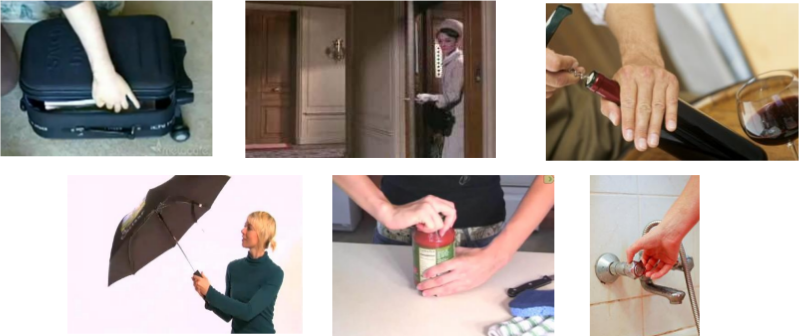
\includegraphics[scale=0.3]{open_example}
  \caption{Παραδείγματα της δράσης «Ανοίγω»}
  \label{fig:open_example}

\end{figure}

Προκειμένου να αντιμετωπιστούν αυτές οι προκλήσεις, έχουν δημιουργηθεί διάφορα σύνολα δεδομένων για ανθρώπινες δράσεις, προκειμένου να αναπτυχθούν
ισχυρά συστήματα αναγνώρισης της ανθρώπινης δράσης και αλγόριθμοι ανίχνευσης.
Τα πρώτα σύνολα δεδομένων περιέλαμβαν έναν δρων χρησιμοποιώντας  μιας στατικής κάμερα πάνω σε ομοιογενή υπόβαθρα.
Παρόλο που αυτά τα σύνολα δεδομένων συνείσφεραν στο να σχεδιάσουμε τους πρώτους αλγορίθμους αναγνώρισης δράσης, δεν ήταν σε θέση να αντιμετωπίσουν αποτελεσματικά τις παραπάνω
προκλήσεις.
Έτσι λοιπόν οδηγηθήκαν στον να δημιουργήσουμε σύνολα δεδομένων που περιέχουν πιο αμφιλεγόμενα βίντεο, όπως το \en Joint-annotated Human Motion Database(JHMDB) (\cite{Kuehne11}) \gr 
και \en UCF-101 (\cite{soomro2012ucf101})\gr. Αυτά τα \en dataset \gr περιλαμβάνουν μόνο ανθρώπινες ενέργειες, η δεύτερη κατηγορία που αναφέρθηκε πιο πριν.

\subsection{\tl{JHMDB Dataset}}
Το σύνολο δεδομένων \en JHMDB (\cite{Jhuang:ICCV:2013}) \gr είναι ένα πλήρες σχολιασμένο σύνολο δεδομένων για ανθρώπινες ενέργειες και ανθρώπινες πόζες. Αποτελείται από 21 κατηγορίες δράσεων
και 928 κλιπ που εξάγονται από την βάση δεδομένων κίνησης του ανθρώπου \en (HMDB51 \cite{Kuehne11})\gr. Αυτό το σύνολο δεδομένων περιέχει κομμένα βίντεο με διάρκεια μεταξύ
15 έως 40 καρέ. Κάθε κλιπ σχολιάζεται για κάθε καρέ χρησιμοποιώντας μια δισδιάστατη στάση και περιέχει μόνο 1 ενέργεια.
Προκειμένου να εκπαιδεύσουμε το μοντέλο μας για τον εντοπισμό των ενεργειών, τροποποιούμε της δισδιάστατες πόζες σε δισδιάσταστα πλαίσια που περιέχουν ολόκληρη τη στάση του δρώντα σε κάθε καρέ.
Υπάρχουν διαθέσιμα 3 διαφορετικά χωρίσματα για να εκπαιδευτεί ένα μοντέλο, τα οποία προτείνουν οι συγγραφείς. Επιλέξαμε το πρώτο  που περιέχει 660
βίντεο στο εκπαιδευτικό σετ και 268 για επικύρωση.

\subsection{\tl{UCF-101 Dataset}}
Το σύνολο δεδομένων \en UCF-101 (\cite{soomro2012ucf101}) \gr περιέχει 13320 βίντεο από 101 κατηγορίες δράσεων.
Από αυτά, παρέχονται χωροχρονικοί  σχολιασμοί για 24 κλάσεις  και 3194 βίντεο. Αυτό σημαίνει ότι σε κάθε βίντεο, υπάρχει ένα \en 2D \gr οριοθετημένο πλαίσιο που περιβάλλει
το άτομο που δρα για κάθε καρέ στο οποίο λαμβάνει χώρα μια δράση.
Διαχωρίζουμε το σύνολο των δεδομένων  σε 2284 βίντεο για εκπαιδευτικό σετ και 910 για σετ επικύρωσης σύμφωνα με το
πρώτο προτεινόμενο διαχωρισμό. Για τα δεδομένα εκπαίδευσης, υπάρχουν βίντεο μέχρι 641 καρέ, ενώ για τα βίντεο επικύρωσης ο μέγιστος αριθμός πλαισίων είναι 900.
Κάθε βίντεο, τόσο για την εκπαίδευση όσο και για την επικύρωση, είναι μη-κομμένο(\en untrimmed\gr), ενώ σε πολλές περιπτώσεις  περισσότερες από 1 ενέργειες πραγματοποιούνται ταυτόχρονα.
Λάβαμε σχολιασμούς από \en \cite{singh2016online} \gr επειδή εκείνουν που μας παρείχαν οι συγγραφείς περιείχαν ορισμένα λάθη.

\section{\enMotivation and Contibutions\gr}
Τα τρέχοντα επιτεύγματα στα δίκτυα αναγνώρισης αντικειμένων και στα \en 3D Convolutional NN για  αναγνώριση ενεργειών μας προκάλεσαν να δοκιμάσουμε
για να τα συνδυάσουμε, προκειμένου να επιτύχουμε τα καλύτερα αποτελέσματα στο πρόβλημα του εντοπισμoύ ανθρώπινης δράσης. Εισάγουμε μια νέα δομή δικτύου εμπνευσμένη από το
\cite{DBLP:journals/corr/HouCS17}, \cite{DBLP:journals/corr/abs-1712-09184}, \cite{Ren:2015:FRT:2969239.2969250} και η υλοποίηση από το  \cite{jjfaster2rcnn}.

Οι συνεισφορές μας είναι οι εξής: 1) Δημιουργούμε ένα νέο \en framework \gr για τον εντοπισμό των ενεργειών που επεκτείνει τον κώδικα που έχει υλοποιηθεί το \en FasterR-CNN,
2) Δημιουργήσαμε ένα δίκτυο για  πρόταση ακολουθιών δυσδιάσταστων κουτιών σε βίντεο κλιπ τα οποία μπορεί να περιέχουν μια δράση, εκμεταλλευόμενοι 
τα χωροχρονικά χαρακτηριστικά που μας παρέχουν οι \en 3D Convolutions\gr, 3) δημιουργούμε έναν αλγόριθμο σύνδεσης για τη σύνδεση των προτεινόμενων ακολουθιών
για να εξάγουμε υποψήφια \en action tubes \gr και 4) προσπαθήσαμε να βρούμε τους καταλληλότερους χάρτες χαρακτηριστικών καθώς και τον κατάλληλο ταξινομητή για να
πραγματοποιήσουμε αποδοτικό \en classification\gr.
\section{\en Thesis structure\gr}
\textbf{NA to ksanadw...}
Η υπόλοιπη διατριβή οργανώνεται ως εξής. Το κεφάλαιο 2 παρέχει μια γενική εισαγωγή στις τεχνικές μηχανικής μάθησης  που χρησιμοποιούνται σήμερα.
Στη συνέχεια, παρουσιάζουμε τα βασικά στοιχεία των συστημάτων αναγνώρισης αντικειμένων παράλληλα με τις συναρτήσεις κόστους  και τις μετρικές που χρησιμοποιήσαμε.
Επίσης, το Κεφάλαιο 2 παρουσιάζει μια σύντομη επισκόπηση της βιβλιογραφίας σχετικά με την αναγνώριση και τον εντοπισμό της ανθρώπινης δράσης.
Το Κεφάλαιο 3 εισάγει το πρώτο βασικό στοιχείο του δικτύου μας, το \en Tube Proposal Network (TPN)\gr, ένα δίκτυο που προτείνει \en Tubes of Interest (ToIs)\gr,
οι οποίες είναι ακολουθίες δυσδιάστατων πλαισίων, που είναι πιθανά να περιέχουν μια εκτελεσθείσα ενέργεια.
Επιπλέον, παρουσιάζονται  όλες τις προτεινόμενες από μας αρχιτεκτονικές για την επίτευξη αυτού του στόχου.
Το κεφάλαιο 4 προτείνει αλγόριθμους για τη σύνδεση των προτεινόμενων \en ToIs \gr από κάθε τμήμα βίντεο και παρουσιάζονται οι επιδόσεις των προτάσεων.
Στο Κεφάλαιο 5 παρουσιάζουμε όλες τις προσεγγίσεις ταξινόμησης που χρησιμοποιήσαμε για τον σχεδιασμό της αρχιτεκτονικής μας και ορισμένα αποτελέσματα ταξινόμησης.
Το Κεφάλαιο 6 χρησιμοποιείται για συμπεράσματα, περίληψη της συμβολής μας μαζί με πιθανές μελλοντικές εργασίες.

% \end{document}

% \documentclass{report}

% \usepackage[greek,english]{babel}

% \newcommand{\tl}{\textlatin}
% \newcommand{\en}{\selectlanguage{english}}
% \newcommand{\gr}{\selectlanguage{greek}}

% \usepackage{hyperref}  % package for linking figures etc
% \usepackage{enumitem}  % package for description with bullets
% \usepackage{graphicx}  % package for importing images
% \usepackage{mathtools} % package for math equation
% \usepackage{mathrsfs}  % package for math font
% \usepackage{indentfirst} % package for getting ident after section or paragraph
% \usepackage{subcaption} % package for subfigures
% \usepackage[export]{adjustbox}
% \usepackage{longtable} % package for multi pages tables
% \usepackage{multirow}  % package for tables, multirow
% \usepackage{amssymb}
% \usepackage{esvect}
% \usepackage[
% backend=bibtex,
% citestyle=authoryear,
% % citestyle=authoryear-comp,
% % citestyle=authoryear-ibid,
% bibstyle=numeric,
% sorting=ynt,
% % style=numeric,
% % style=alphabetic ,
% ]{biblatex}
% \addbibresource{References}

% \graphicspath{ {./theory/figures/} }       % path for images

% \begin{document}
\gr
\chapter{Σχετική βιβλιογραφία}
Σε αυτή την ενότητα, παρουσιάζουμε ορισμένες από τις πιο συναφείς μεθόδους για την εργασία μας και άλλες που μελετήθηκαν για τον σχεδιασμό αυτής της προσέγγισης.
Οι μέθοδοι αυτές  χωρίζονται σε δύο ενότητες \textit{Aναγνώριση Δραστηριότητας} και \textit{Εντοπισμός Δραστηριότητας}. Το πρώτο μέρος αναφέρεται σε κλασικές μεθόδους
ταξινόμησης δράσης που εισήχθησαν μέχρι πρόσφατα και το δεύτερο μέρος, αντίστοιχα, σε πρόσφατες μεθόδους εντοπισμού της δράσης. 

\subsection{Αναγνώριση Δραστηριότητας}
Οι πρώτες προσεγγίσεις για την κατάταξη της δράσης αποτελούνταν από δύο βήματα α) αρχικά υπολογισμός σύνθετων «χειροποίητων» χαρακτηριστικών από ακατέργαστα καρέ βίντεο
και β) εκπαίδευση ενός ταξινομητή με βάση αυτά τα χαρακτηριστικά. Αυτά τα χαρακτηριστικά μπορούν να διαχωριστούν σε 3 κατηγορίες:
1) προσεγγίσεις χωροχρονικού όγκου \tl{(space-time volume)}, 2) τροχιές \tl{(trajectories)} και 3) χωροχρονικά  χαρακτηριστικά. Για τις μεθόδους χωροχρονικού όγκου,
η προσέγγιση είναι η εξής: Με βάση τα \tl{training} βίντεο, το σύστημα συνάπτει ένα μοντέλο τρισδιάστατου χωροχρόνου, συνενώνοντας δισδιάστατες εικόνες
(διάσταση \tl{\textit{x-y}}) κατά τη διάρκεια του χρόνου (διάσταση \tl{\textit{t}} ή \tl{\textit{z}}), για την αναπαράσταση κάθε δράσης.
Όταν το σύστημα δέχεται ένα βίντεο που δεν έχει ετικέτα, κατασκευάζει μια τρισδιάστατη χωροχρονική αναπαράσταση που αντιστοιχεί σε αυτό το βίντεο.
Αυτό η νέα τρισδιάστατη αναπαράσταση, στη συνέχεια, συγκρίνεται με κάθε μοντέλο \tl{3D} χωροχρόνου, συγκρίνοντας την ομοιότητα στο σχήμα
και την εμφάνιση μεταξύ αυτών των δύο χωροχρονικών όγκων.
Το σύστημα εξάγει την κατηγορία του άγνωστου βίντεο, αντιστοιχώντας την με αυτήν της δράσης με την υψηλότερη ομοιότητα. Επιπλέον, υπάρχουν
διάφορες παραλλαγές των  χωροχρονικών αναπαραστάσεων. Αντί της αναπαράστασης \tl{space-time volume}, το σύστημα μπορεί να αναπαριστά τη κάθε δράση ως τροχιές
σε χωροχρονικές διαστάσεις ή ακόμη περισσότερο, η ενέργεια μπορεί να αναπαρασταθεί ως ένα σύνολο χαρακτηριστικών που εξάγονται από τον χωροχρονικό όγκο ή τις τροχιές.
Οι «καθαρές» χωροχρονικές αναπαραστάσεις περιλαμβάνουν μεθόδους σύγκρισης των περιοχών προσκηνίου ενός ατόμου (δηλ. σιλουέτες) όπως των \en \cite{BobickAaron},\gr
συγκρίνοντας όγκους σε σχέση με επιφάνεια τους όπως οι \en \cite{1467296}\gr. Η μέθοδος των \en \cite{4270510}\gr χρησιμοποιεί \tl{oversegmented} όγκους, αυτομάτως
υπολογίζοντας ένα σύνολο τμημάτων τρισδιάστατου όγκου \tl{ XYT} που αντιστοιχεί σε έναν κινούμενο άνθρωπο. Οι \en\cite{4587727} \gr πρότειναν φίλτρα για
να αποτυπώνουν τα χαρακτηριστικά του χωροχρονικού όγκου, προκειμένου να τα ταιριάζουν πιο αξιόπιστα και αποδοτικά.
Από την άλλη πλευρά, οι προσεγγίσεις με βάση την τροχιά περιλαμβάνουν την αναπαράσταση μιας ενέργειας ως σύνολο 13 κοινών διαδρομών (\en\cite{1541250}\gr) ή
τη χρήση ενός συνόλου \tl{\textit{XYZT}}-διαστάσεων κοινών τροχιών που λαμβάνονται από κινούμενες κάμερες  (\en\cite{1541251}\gr).
Τέλος, διάφορες μέθοδοι χρησιμοποιούν τοπικά χαρακτηριστικά που εξάγονται από χωροχρονικούς όγκους τριών διαστάσεων,
όπως η εξαγωγή τοπικών χαρακτηριστικών σε κάθε καρέ του βίντεο και η ένωση τους χρονικά (\en\cite{784616, 990935, 1544882}\gr,
η εξαγωγή αραιών χωροχρονικών τοπικών σημείων ενδιαφέροντος από τρισδιάστατους όγκους (\en\cite{1238378, 1570899,  Niebles, 1467373, Ryoo2006}\gr)
Οι προσεγγίσεις αυτές κατέστησαν την επιλογή των χαρακτηριστικών  σημαντικό παράγοντα για την απόδοση του δικτύου.
Αυτό συμβαίνει επειδή οι διαφορετικές κατηγορίες δράσεων μπορεί να διαφέρουν δραματικά από την άποψη της εμφάνισής τους και των μοτίβων κίνησης.
Ένα άλλο πρόβλημα ήταν ότι οι περισσότερες από αυτές τις προσεγγίσεις κάνουν υποθέσεις, υπό τις οποίες το βίντεο λήφθηκε λόγω προβλημάτων όπως το γεμάτo
φόντο,  γωνιές κάμερας κλπ. Μια ανασκόπηση των τεχνικών, που χρησιμοποιούνταν  μέχρι το 2011, παρουσιάζεται απ' τους\en\cite{Aggarwal:2011:HAA:1922649.1922653}\gr.  \par

Τα πρόσφατα αποτελέσματα σε βαθιές αρχιτεκτονικές και ειδικά στον τομέα της ταξινόμησης εικόνας  έδωσε κίνητρο στους ερευνητές να εκπαιδεύσουν δίκτυα \tl{CNN} για
το πρόβλημα της αναγνώρισης δράσης. Η πρώτη σημαντική απόπειρα έγινε από τους \en\cite{6909619}\gr. Σχεδίασαν την αρχιτεκτονική τους με βάση το καλύτερο \tl{CNN}
στον διαγωνισμό  \tl{ImageNet}.
Εξερευνούν διάφορες μεθόδους για τη σύντηξη των χωροχρονικών λειτουργιών χρησιμοποιώντας δισδιάστατες διαδικασίες κυρίως και τρισδιάστατη συνέλιξη μόνο μέσω αργής σύντηξης.
Οι \en \cite{simonyan2014two} \gr χρησιμοποίησαν 2 \en CNNs\gr, ένα για χωρικές πληροφορίες και ένα για οπτική ροή
και τα συνδύασαν  με τη χρήση της καθυστερημένης σύντηξης. Δείχνουν ότι η εξόρυξη χωρικού περιεχομένου από τα βίντεο και περιεχόμενο κίνησης από την οπτική ροή μπορεί να βελτιώσει
σημαντικά την ακρίβεια της αναγνώρισης της δράσης. Οι \en\cite{DBLP:journals/corr/FeichtenhoferPZ16} \gr επέκτειναν αυτή την προσέγγιση με τη χρήση πρώιμης σύντηξης στο τέλος των \en convolutional
layers \gr αντί της  καθυστερημένης σύντηξης, η οποία λαμβάνει χώρα στο τελευταίο επίπεδο του δικτύου. Πάνω σ' αυτό, χρησιμοποίησαν ένα δεύτερο δίκτυο για το χρονικό περιεχόμενο το οποίο
συνδέουν με το το άλλο δίκτυο με χρήση της καθυστερημένης σύντηξης. Επιπλέον, οι \en \cite{DBLP:journals/corr/WangXW0LTG16} \gr στήριξαν την μέθοδος τους
σε αυτήν που πρότειναν οι \en \cite{simonyan2014two}\gr. Ασχολούνται με το πρόβλημα  της εύρεσης χρονικού περιεχομένου και εκπαιδεύουν το δίκτυο τους, παρέχοντας του λίγα δείγματα.
Η προσέγγισή τους, την οποία ονόμασαν \en Temporal Segment Network (TSN), \gr διαχωρίζει το βίντεο εισόδου σε K τμήματα  και ένα σύντομο απόσπασμα από κάθε τμήμα επιλέγεται για ανάλυση.
Στη συνέχεια, συνδέουν  το εξαγόμενο χωροχρονικό περιεχόμενο, πραγματοποιώντας τελικά την πρόβλεψή τους. Πιο πρόσφατα, οι \en \cite{DBLP:journals/corr/ZhangWWQW16} \gr και οι \en \cite{DBLP:journals/corr/ZhuLNH17a} \gr χρησιμοποίησαν την \en two-stream \gr προσέγγιση, επίσης. Οι \en \cite{DBLP:journals/corr/ZhangWWQW16} \gr αντικατέστησαν την οπτική ροή με ένα διάνυσμα κίνησης που μπορεί να ληφθεί απευθείας
από τα  συμπιεσμένα βίντεο χωρίς επιπλέον υπολογισμό και το τροφοδοτούν στο δίκτυο. Οι \en  \cite{DBLP:journals/corr/ZhuLNH17a} \gr εκπαίδευσαν ένα  \en CNN  \gr για τον υπολογισμό της οπτικής ροής,
καλώντας το, \en MotionNet \gr, και χρησιμοποίησαν ένα \en CNN \gr ως  χρονικό \en stream \gr για προβάλλουν τις πληροφορίες κίνησης έργου σε κατηγορίες δράσεων. Τέλος
χρησιμοποιούν την καθυστερημένη σύντηξη μέσω της μέσης τιμής με βάρη τα σκορ πρόβλεψης των χρονικών και χωρικών \en stream\gr. Από την άλλη πλευρά, μια νέα προσέγγιση εισήχθη από τους
\en\cite{DBLP:journals/corr/abs-1711-01467}\gr ενσωματώνοντας χάρτες προσοχής με σκοπόν να βελτιώσουν σημαντικά  την απόδοση της αναγνώρισης δράσης. \par

Ορισμένες άλλες μέθοδοι περιλάμβαναν ένα δίκτυο \en RNN \gr  ή  \en LSTM  \gr για την ταξινόμηση όπως κάνουν οι \en\cite{DBLP:journals/corr/DonahueHGRVSD14}\gr, οι \en \cite{DBLP:journals/corr/NgHVVMT15} \gr
και οι \en \cite{DBLP:journals/corr/MaCKA17}\gr. Οι  \en \cite{DBLP:journals/corr/DonahueHGRVSD14}\gr αντιμετωπίζουν τηv  πρόκληση των μεταβλητών μεγεθών των ακολουθιών εισόδου και εξόδου,
εκμεταλλευόμενοι τα \en convolutional layers \gr  και τις μεγάλου εύρους χρονικές αναδρομές (\en recursions\gr). Προτείνουν ένα \en Long-term Recurrent
Convolutional Network (LRCN)\gr, το οποίο είναι ικανό να αντιμετωπίσει  τις εργασίες αναγνώρισης, λεζάντας εικόνας και περιγραφής βίντεο.
Για να ταξινομήσει μια δεδομένη ακολουθία καρέ, το \en LRCN \gr λαμβάνει αρχικά ως είσοδο ένα καρέ, και πιο συγκεκριμένα τα κανάλια \en RGB \gr και την οπτική ροή του, και προβλέπει μια ετικέτα.
Μετά από αυτό, εξάγει την  κλάση  του βίντεο μέσω του  μέσου όρου των πιθανοτήτων των ετικετών, επιλέγοντας την πιο πιθανή κλάση.
Οι  \en\cite{DBLP:journals/corr/NgHVVMT15}  \gr πρώτα διερευνούν  διάφορες προσεγγίσεις για χρονική ομαδοποίηση (\en temporal pooling\gr) των χαρακτηριστικών.
Αυτές οι τεχνικές περιλαμβάνουν τον χειρισμό καρέ βίντεο ξεχωριστά από 2 αρχιτεκτονικές \en  CNN\gr: είτε απ' το \en AlexNet \gr είτε απ' το \en GoogleNet\gr, και αποτελούνται από 
πρώιμη σύντηξη, καθυστερημένη σύντηξη και  ενός συνδυασμού αυτών. Επιπλέον, προτείνουν ένα \en RNN \gr προκειμένου να εξετάσουν τα βίντεο κλιπ
ως ακολουθίες ενεργοποιήσεων \en CNN\gr. Το προτεινόμενο \en LSTM \gr λαμβάνει ως είσοδο την έξοδο του τελικού \en CNN layer \gr για κάθε συνεχόμενο καρέ και μετά από 5 \en LSTM layers \gr και χρησιμοποιώντας
έναν \en softmax \gr ταξινομητή, προτείνει μία ετικέτα. Για την ταξινόμηση του βίντεο,  επιστρέφουν μια ετικέτα μετά το τελευταίο βήμα, εφαρμόζουν \en max-pooling \gr στις προβλέψεις στην διάσταση
του χρόνου, αθροίζουν τις προβλέψεις στην διάσταση του χρόνου και επιστρέφουν το μέγιστο ή έναν γραμμικό συνδυασμό με βάρη των προβλέψεων υπό έναν παράγοντα \tl{g}, τα αθροίζουν και επιστρέφουν το μέγιστο.
Έδειξαν ότι όλες οι προσεγγίσεις είναι 1\% διαφορετικές με προκατάληψη για τη χρήση των προβλέψεων με βάρη 
για την υποστήριξη της ιδέας ότι το \en LSTM \gr γίνεται προοδευτικά πιο ενημερωμένο. Τελευταίοι 
αλλά όχι λιγότερο σημαντικοί, οι \en \cite{DBLP:journals/corr/MaCKA17} \gr χρησιμοποίησαν ένα \en two-stream ConvNet \gr για  εξαγωγή χαρακτηριστικών και είτε ένα \en
LSTM \gr ή  \en convolutional layer \gr πάνω από τους χρονικώς κατασκευασμένους πίνακες χαρακτηριστικών για τη σύντηξη χωρικών και χρονικών πληροφοριών. Χρησιμοποιούν ένα \en ResNet-101 \gr
για την εξόρυξη χαρτών ενεργοποίησης  τόσο για χωρικές όσο και για χρονικές ροές. Χωρίζουν το 
βίντεο σε διάφορα τμήματα, όπως έκαναν οι \en \cite{DBLP:journals/corr/WangXW0LTG16}\gr, και χρησιμοποίησαν ένα επίπεδο  \en temporal pooling \gr για την εξαγωγή διακεκριμένων χαρακτηριστικών.
Αφού λάβουν αυτά τα χαρακτηριστικά, το \en LSTM  \gr
εξάγει ενσωματωμένες δυνατότητες από όλα τα τμήματα. \par


Επιπλέον, οι \en \cite{Tran2014LearningSF} \gr  διερεύνησαν τα \en  3D Convolutional \gr δίκτυα (\en \cite{pmid:22392705}\gr)
και εισήγαγαν το \en  C3D \gr δίκτυο που έχει \en  3D convolutional layers \gr  με πυρήνες $3 \times  3 \times 3$.
Αυτό το δίκτυο είναι σε θέση να μοντελοποιήσει την  εμφάνιση και την κίνηση ταυτόχρονα χρησιμοποιώντας τρισδιάστατες συνελίξεις και μπορεί να χρησιμοποιηθεί ως
εξαγωγέας χαρακτηριστικών. Συνδυάζοντας την αρχιτεκτονική δύο ροών και τις τρισδιάσττες συνελίξεις οι \en\cite{DBLP:journals/corr/CarreiraZ17}  \gr πρότειναν το  δίκτυο \en I3D\gr.
Πάνω σ' αυτό, oι δημιουργοί τονίζουν τα πλεονεκτήματα της μεταφοράς μάθησης για την εργασία της αναγνώρισης επαναλαμβάνοντας τα δισδιάστατα προ-εκπαιδευμένα βάρη στην 3η διάσταση.
Οι \en \cite{DBLP:journals/corr/abs-1708-07632} \gr πρότειναν ένα δίκτυο \en 3D ResNet \gr για την αναγνώριση δράσης με βάση τα \en Residual \gr δίκτυα (\en ResNet)(\cite{DBLP:journals/corr/HeZRS15}\gr)
και διερευνούν την απόδοση  των δικτύων \en ResNet \gr με  \en 3D Convolutional \gr πυρήνες. Από την άλλη, οι \en \cite{DBLP:journals/corr/abs-1711-08200} \gr 
βάσισαν  την προσέγγισή τους στα \en DenseNets (\cite{DBLP:journals/corr/HuangLW16a}) \gr και επέκτειναν την αρχιτεκτονική του \en DenseNet \gr χρησιμοποιώντας τρισδιάστατα φίλτρα
και \en pooling \gr πυρήνες αντί για δισδιάστατους, ονομάζοντας αυτή την προσέγγιση ως \en DenseNet3D\gr. Επιπλέον, εισάγουν το \en Layer \gr χρονικής μετάβασης \en(TTL)\gr,
το οποίο συνενώνει χρονικά χάρτες χαρακτηριστικών που εξάγονται  σε διαφορετικά  χρονικά βάθη και αντικαθιστά το επίπεδο μετάβασης του \en  DenseNet\gr.
Παράλληλα, οι \en \cite{DBLP:DibaFSKAYG18} \gr εισήγαγαν  ένα νέο χρονικό \en layer \gr το οποίο μοντελοποιεί  μεταβλητούς χρονικούς  πυρήνες συνέλιξης. Τελευταίοι αλλά εξίσου σημαντικοί, 
oi \en \cite{DBLP:journals/corr/abs-1711-11248} \gr  πειραματίστηκαν  με διάφορες υπόλοιπες αρχιτεκτονικές \en Residual \gr δικτύου χρησιμοποιώντας
συνδυασμούς \en 2D  \gr και \en 3D convolutional Layer\gr. Σκοπός τους είναι να δείξουν ότι η \en 2D \gr χωρική συνέλιξη ακολουθούμενη από \en 1D \gr χρονική  συνέλιξη επιτυγχάνει \en state-of-the-art \gr
αποτελέσματα, ονομάζοντας αυτού του τύπου το \en layer \gr ως \en R(2 + 1)D\gr. Πρόσφατα οι \en \cite{Guo_2018_ECCV} \gr  πρότειναν ένα \en framework \gr  που μπορεί να μάθει να
 αναγνωρίζει μια προηγουμένως αθέατη \en 3D \gr κλάση δράσης  με λίγα μόνο παραδείγματα εκμεταλλευόμενο την εγγενή δομή των \en 3D \gr δεδομένων μέσω μιας γραφικής αναπαράστασης.
Ακόμα πιο λεπτομερή  παρουσίαση των τεχνικών αναγνώρισης δράσης που χρησιμοποιήθηκαν μέχρι το 2018 πραγματοποιήθηκε από τους \en\cite{DBLP:journals/corr/abs-1806-11230}\gr.

\subsection{Εντοπισμός Δραστηριότητας}

Όπως προαναφέρθηκε, ο εντοπισμός δράσης μπορεί να θεωρηθεί ως προέκταση του
προβλήματος εντοπισμού αντικειμένων. Αντί να εξάγουμε δισδιάστατα πλαίσια οριοθέτησης  σε μία μόνο
εικόνα, ο στόχος των συστημάτων εντοπισμού δράσης είναι να εξάγουν \en action tubes, \gr τα οποία 
είναι ακολουθίες πλαισίων οριοθέτησης που περιέχουν μια ενέργεια που εκτελέστηκε. Έτσι, υπάρχουν
διάφορες προσεγγίσεις, συμπεριλαμβανομένου συνήθως ενός δικτύου ανιχνευτή αντικειμένων  και ενός ταξινομητή. \par

Οι πρώτες προσεγγίσεις ανίχνευσης αντικειμένων περιλάμβαναν την επέκταση ενός αλγορίθμου  πρότασης αντικειμένων
σε 3 διαστάσεις. Οι \en\cite{6619185} \gr επέκτείναν τα παραμορφώσιμα (\en deformable) \gr μοντέλα (\en\cite{5255236}\gr) με το να αντιμετωπίζουν τις δράσεις  ως
χωροχρονικά μοτίβα και  δημιούργησαν ένα παραμορφώσιμου μοντέλο για κάθε δράση. Oi \en \cite{6909495} \gr εισήγαγαν την έννοια των \en tubelets\gr, γνωστά και ως ακολουθίες
πλαισίων οριοθέτησης και βάσισαν τη μέθοδό τους σε επιλεκτικό αλγόριθμο αναζήτησης (\en\cite{Uijlings13}\gr), επεκτείνοντας τα \en superpixels \gr σε \en supervoxels \gr
για την παραγωγή χωροχρονικών σχημάτων. Απ' την άλλη, οι \en \cite{Oneata} \gr επέκτειναν  μια τυχαιοποιημένη διαδικασία συγχώνευσης \en superpixels \gr 
που χρησιμοποιούνταν  για προτάσεις  αντικειμένων, όπως παρουσιάστηκαν απ' τους \en \cite{Manen:2013:POP:2586117.2587333}\gr.
Οι \en\cite{7298735} \gr  πρώτα προτείνουν πλαίσια οριοθέτησης για κάθε καρέ με χρήση ενός ανιχνευτή ανθρώπου  και κίνησης, ενώ, στη συνέχεια, με τη επιλογή των καλύτερων σε σκορ κουτιών,
πρότειναν έναν άπληστο συνδετικό αλγόριθμο με τη διατύπωση την εργασίας σύνδεσης ως  πρόβλημα  μέγιστης κάλυψης. Οι \en \cite{BMVC2015_177} \gr παράγουν  χωροχρονικές προτάσεις κατευθείαν
από τις πυκνές τροχιές, οι οποίες επίσης χρησιμοποιήθηκαν για ταξινόμηση.
Οι \en\cite{7410734} \gr δημιουργούν ένα γράφημα χωροχρονικής τροχιάς και επιλέγουν προτάσεις δράσεων που βασίζονται μόνο στην εσκεμμένη κίνηση που εξάγεται από το γράφημα.
Οι \en\cite{7410732} \gr διαχωρίζουν  τα τμήματα βίντεο σε \en supervoxels \gr και  χρησιμοποιούν το περιεχόμενο τους ως χωρική σχέση μεταξύ των \en supervoxels \gr σε σχέση με την δράση του προσκηνίου.
Δημιουργούν ένα γράφημα για κάθε βίντεο, όπου τα \en supervoxels \gr σχηματίζουν τους κόμβους και οι  κατευθυνόμενες άκρες απεικονίζουν  τις χωρικές σχέσεις μεταξύ τους. Κατά τη διάρκεια των δοκιμών,
κάνουν μια βόλτα στο περιβάλλον, όπου κάθε βήμα καθοδηγείται από τις σχέσεις περιβάλλοντος κατά τη διάρκεια της εκπαίδευσης, με αποτέλεσμα μια κατανομή  πιθανότητας μιας δράσης για όλα τα \en supervoxels\gr.
Οι \en\cite{DBLP:journals/corr/MettesGS16} \gr αντί για τοποθέτηση  πλαισίων σε όλα τα καρέ των βίντεο, σχολίασαν σημεία σε ένα αραιό  υποσύνολο καρέ του  βίντεο και χρησιμοποίησαν
προτάσεις που λαμβάνονται μέσω ενός μέτρου επικάλυψης μεταξύ των προτάσεων δράσης και των σημείων.
Οι \en\cite{DBLP:journals/corr/BehlSSSCT17} \gr ασχολούνται με  την ανίχνευση και τον εντοπισμό  ενεργειών σε πραγματικό χρόνο μέσω της λήψης προτάσεων δράσης ανά καρέ και την πρόταση ενός αλγορίθμου
σύνδεσης που είναι σε θέση να κατασκευάσει και να ενημερώνει τα \en action tubes \gr ανά καρέ. Πιο πρόσφατα, οι  \en\cite{8237344} \gr προσπάθησαν  να ασχοληθούν  με το πρόβλημα της ανίχνευσης και
τον εντοπισμό δράσης χωρίς επίβλεψη. Η προσέγγισή τους περιελάμβανε αρχικά την εξόρυξη  κατακερματισμένων \en supervoxel \gr
και στη συνέχεια την ανάθεση ενός βάρους σε κάθε \en supervoxel\gr. Με την εξαγωγή \en supervoxels\gr, δημιουργούν ένα γράφημα και
στη συνέχεια χρησιμοποιούν μια διακριτική \en clustering \gr προσέγγιση έτσι ώστε να εκπαιδεύεται ένας ταξινομητής.

Η εισαγωγή του \en R-CNN (\cite{DBLP:journals/corr/GirshickDDM13}) \gr κατάφερε σημαντικές βελτιώσεις
στην  απόδοση των δικτύων εντοπισμού αντικειμένων. Αυτή η αρχιτεκτονική,
πρώτον, προτείνει περιοχές στην εικόνα που είναι πιθανό να περιέχουν κάποιο αντικείμενο και
στη συνέχεια, τα ταξινομεί χρησιμοποιώντας ένα \en SVM\gr. Εμπνευσμένοι από αυτή την αρχιτεκτονική,
οι \en \cite{DBLP:journals/corr/GkioxariM14} \gr σχεδίασαν ένα δίκτυο \en RCNN 2-stream \gr για να προτείνει 
προτάσεις δράσεων  για κάθε καρέ, ένα \en stream \gr για το επίπεδο καρέ και ένα για την 
οπτική ροή. Στη συνέχεια, τα συνδέουν χρησιμοποιώντας τον αλγόριθμο σύνδεσης \en Viterbi\gr.
Οι \en \cite{DBLP:journals/corr/WeinzaepfelHS15} \gr επεκτείνουν αυτή την προσέγγιση, εκτελώντας
προτάσεις στο επίπεδο καρέ  και χρησιμοποιώντας ένα \en tracker \gr για τη σύνδεση των προτάσεων αυτών μέσω των
χαρακτηριστικών της χωρικής και οπτικής ροής. Επίσης, η μέθοδός τους εκτελεί χρονικό εντοπισμό μέσω της χρήσης
ενός συρόμενου παράθυρου πάνω από τα εντοπισμένα \en tubes\gr.   \par

Η εισαγωγή του \en Faster RCNN (\cite{Ren:2015:FRT:2969239.2969250}) \gr συνείσφερε  πολύ
τη βελτίωση της απόδοσης των δικτύων εντοπισμού δράσης. Οι \en\cite{peng:hal-01349107} \gr και \en\cite{DBLP:journals/corr/SahaSSTC16} \gr 
χρησιμοποιούν το \en Faster R-CNN \gr αντί για το \en  RCNN \gr  για προτάσεις σε επίπεδο καρέ, χρησιμοποιώντας το \en RPN \gr για εικόνες \en RGB \gr και οπτικής ροής.
Αφού λάβουν χωρικές προτάσεις και προτάσεις κίνησης, οι \en \cite{peng:hal-01349107} \gr τις συγχωνεύουν και από κάθε προτεινόμενη \en ROI\gr, παράγουν 4 \en ROIs \gr για να επικεντρωθούν
σε συγκεκριμένο μέρος του σώματος του δρώντα. Μετά από αυτό, συνδέουν την πρόταση χρησιμοποιώντας τον αλγόριθμο \en Viterbi \gr για κάθε κλάση και εκτελούν χρονικό εντοπισμό
χρησιμοποιώντας ένα συρόμενο παράθυρο, με πολλαπλές χρονικές κλίμακες και διασκελισμό κάνοντας χρήση  μιας μεθόδου  μέγιστης υποσυστοιχίας (\en maximum subarray method\gr).
Απ' την άλλη, οι \en \cite{DBLP:journals/corr/SahaSSTC16} \gr εκτελούν, επίσης, ταξινόμηση σε επίπεδο καρέ. Μετά απ' αυτό,  η μέθοδός τους εκτελεί σύντηξη με βάση έναν συνδυασμό
της εμφάνισης και της κίνησης με βάση τις προτάσεις και την βαθμολογία αλληλεπικάλυψης. Τέλος, η χρονική προσαρμογή λαμβάνει χώρα χρησιμοποιώντας δυναμικό προγραμματισμό.
Παράλληλα, οι \en \cite{DBLP:journals/corr/WeinzaepfelMS16} \gr χρησιμοποιούν το \en Faster RCNN \gr
για την εξαγωγή ανθρώπινων \en tubes \gr από βίντεο που εστιάζουν στο πρόβλημα του ασθενώς εποπτευόμενoυ εντοπισμού δράσης.
 Στη συνέχεια, χρησιμοποιώντας πυκνές τροχιές και μια \en multi-fold Multiple  Instance  Learning \gr προσέγγιση \en(\cite{7420739}\gr)  εκπαιδεύουν ένα
 ταξινομητή. Οι \en \cite{DBLP:journals/corr/MettesS17} \gr εισήγαγαν μια μέθοδο για \en zero-shot \gr εντοπισμού δράσης. Η προσέγγισή τους περιλαμβάνει την βαθμολόγηση των προτεινόμενων
 \en action tubes \gr  σύμφωνα με τις αλληλεπιδράσεις μεταξύ των ατόμων που δρουν  και  αντικειμένων. Χρησιμοποίησαν το \en Faster-RCNN\gr,
στο πρώτο βήμα, για την ανίχνευση τόσο των ανθρώπων που δρουν όσο και των αντικειμένων και μετά, χρησιμοποιώντας χωρικές σχέσεις μεταξύ τους,  συνδέουν τα προτεινόμενα πλαίσια στον άξονα του χρόνου
βασιζόμενοι στην \en zero-shot \gr πιθανότητα της παρουσίας των ατόμων, συναφών αντικειμένων γύρω απ' αυτούς και τις αναμενόμενες χωρικές σχέσεις μεταξύ αντικειμένων και ανθρώπων που δρουν. Επιπλέον
οι \en\cite{DBLP:journals/corr/HeIDM17} \gr πρότειναν  το \en Tube Proposal Network (TPN) \gr για τη δημιουργία ανεξαρτήτου κλάσης προτάσεων \en tubelet\gr, οι οποίες χρησιμοποιούν το \en Faster R-CNN \gr
για να λάβουν δισδιάστατες προτάσεις περιοχών και έναν αλγόριθμο σύνδεσης για τη σύνδεση των \en tubelets  \gr με τις  προτάσεις των περιοχών. Πιο πρόσφατα, oi \en \cite{DBLP:journals/corr/abs-1807-10066}
\gr πρότειναν μια μέθοδο για εντοπισμό δράσεων στο σύνολο δεδομένων \en AVA  (\cite{DBLP:journals/corr/GuSVPRTLRSSM17}\gr) συνδυάζοντας τις αρχιτεκτονικές
των \en I3D (\cite{DBLP:journals/corr/CarreiraZ17}\gr) και \en Faster RCNN\gr. Χρησιμοποιούν μπλοκ του \en I3D \gr για την λήψη αναπαράστασης βίντεο και το  \en RPN \gr του \en Faster-RCNN \gr
για να προτείνει προτάσεις «ανθρώπου» για το κεντρικό πλαίσιο. \par

Παράλληλα μ' αυτά, οι \en \cite{singh2016online} \gr και \en\cite{kalogeiton17iccv:hal-01519812} \gr  σχεδίασαν τα δίκτυα τους
με βάση το \en Single Shot Multibox Detector \cite{DBLP:journals/corr/LiuAESR15})\gr. Οι \en\cite{singh2016online} \gr δημιούργησαν
ένα  χωροχρονικό δίκτυο  πραγματικoύ χρόνου. Για να λειτουργεί το δίκτυο τους σε πραγματικό χρόνο, οι \en  \cite{singh2016online} \gr πρότειναν έναν νέο και αποδοτικό
αλγόριθμο με την προσθήκη πλαισίων σε \en tubes \gr σε κάθε καρέ, εάν επικαλύπτονται περισσότερο από ένα κατώφλι, ή  εναλλακτικά, τερματίζουν  το \en action tube \gr εάν για \tl{k} καρέ
αν δεν προστέθηκε κανένα πλαίσιο. Οι \en\cite{kalogeiton17iccv:hal-01519812} \gr  σχεδίασαν ένα δίκτυο δύο ροών, το οποίο κάλεσαν
\en ACT-detector \gr, και εισήγαγαν τα κυβικά (\en cuboids) anchors\gr. Για K καρέ, και για τα δύο δίκτυα,
οι \en \cite{kalogeiton17iccv:hal-01519812} \gr εξάγουν  χωρικά χαρακτηριστικά σε επίπεδο καρέ, στη συνέχεια, τα στοιβάζουν.
Τέλος, με τη χρήση των κυβικών \en anchors\gr, το δίκτυο  εξάγει \en tubelets\gr,
με τις αντίστοιχες βαθμολογίες κατάταξης και στόχους παλινδρόμησης. Για τη σύνδεση των \en tubelets\gr, oi \en \cite{kalogeiton17iccv:hal-01519812} \gr  ακολουθούν 
τα ίδια βήματα με τους \en \cite{singh2016online}\gr, ενώ για χρονικό εντοπισμό, χρησιμοποιούν μιά προσέγγιση χρονικής εξομάλυνσης. \par

Πιο πρόσφατα, το δίκτυο \en YOLO (\cite{DBLP:journals/corr/RedmonDGF15}) \gr έγινε η έμπνευση
για  τους \en \cite{DBLP:journals/corr/abs-1903-00304} \gr και τους \en \cite{DBLP:journals/corr/abs-1802-08362}\gr. Στην προσέγγιση που προτάθηκε από τους
\en  \cite{DBLP:journals/corr/abs-1903-00304}\gr, οι έννοιες της
εξέλιξης και τού ποσοστoύ προόδου εισήχθησαν. Εκτός από την πρόταση πλαισίων οριοθέτησης σε επίπεδο καρέ, χρησιμοποιούν το \en YOLO \gr μαζί με έναν ταξινομητή \en RNN \gr για
να εξάγουν χρονικές πληροφορίες για τις προτάσεις. Με βάση αυτές τις πληροφορίες, δημιουργούν \en action tubes, \gr χωρίζοντας τα  σε κλάσεις. Ορισμένες άλλες προσεγγίσεις περιλαμβάνουν
εκτίμηση πόζας, όπως αυτή των \en \cite{DBLP:journals/corr/abs-1802-09232}\gr. Πρότειναν μια μέθοδο
υπολογισμού των δισδιάστατων και τρισδιάστατων ποζών και στη συνέχεια εκτέλεσαν ταξινόμηση δράσεων.
Χρησιμοποιούν το διαφορίσιμο \en Soft-argamax \gr για   την εκτίμηση των \tl{2D} και \tl{3D}
αρθρώσεων, επειδή η συνάρτηση \en argmax \gr δεν είναι διαφορίσιμη. Στη συνέχεια, για T παρακείμενες πόζες
δημιουργούν μια απεικόνιση εικόνας με το χρόνο και τις $N_j$  αρθρώσεις  ως $x-y$ άξονες, έχοντας  2 κανάλια για την \tl{2D} πόζα  και 3  για την \tl{ 3D} πόζα.
Χρησιμοποιούν \en Convolutional Layers \gr για να παράγουν  χάρτες θερμότητας δράσης   και στη συνέχεια χρησιμοποιώντας \en  max plus min pooling \gr και την συνάρτηση \en softmax \gr
 εκτελούν ταξινόμηση δράσης.
 Οι \en \cite{DBLP:journals/corr/ZolfaghariOSB17} \gr πρότειναν μια αρχιτεκτονική τριών ροών που περιλαμβάνει \en 2D \gr πόζα, οπτική ροή και πληροφορίες \en  RGB\gr. Αυτά τα \en streams \gr ενώνονται
 μέσω του μοντέλου της αλυσίδας \en Markov\gr. Επιπλέον, οι \en \cite{8237881} \gr πρότειναν μια αρχιτεκτονική με τη χρήση ενός χρονικού \en convolutional \gr δικτύου παλινδρόμησης,
 για να πιάνουν την  μακροπρόθεσμη εξάρτηση και πληροφορίες  μεταξύ γειτονικών καρέ και ένα χωρικό δίκτυο παλινδρόμησης, για  προτάσεις ανά καρέ. Χρησιμοποιούν μεθόδους παρακολούθησης
και δυναμικoύ προγραμματισμού για τη δημιουργία προτάσεων δράσης. \par

Τα περισσότερα από τα προαναφερθέντα δίκτυα χρησιμοποιούν ανά καρέ χωρικές προτάσεις και εξάγουν 
τις χρονικές τους πληροφορίες υπολογίζοντας την οπτική ροή. Από την άλλη
oi \en \cite{DBLP:journals/corr/SahaSC17} \gr σχεδίασαν μια αρχιτεκτονική η οποία περιλαμβάνει προτάσεις σε επίπεδο τμήματος βίντεο, το οποίο σημαίνει  περισσότερα από ένα
καρέ ταυτόχρονα. Οι \en \cite{DBLP:journals/corr/SahaSC17} \gr  πρότειναν μια \en 3D-RPN \gr αρχιτεκτονική 
που είναι σε θέση να δημιουργήσει και να ταξινομήσει τρισδιάστατες προτάσεις   αποτελoύμενες από 2 συνεχόμενα  καρέ. Επίσης, πρότειναν έναν αλγόριθμο σύνδεσης,
τροποποιώντας αυτόν που πρότειναν oi \en \cite{DBLP:journals/corr/SahaSSTC16}\gr. Πάνω σ' αυτό, οι \en \cite{DBLP:journals/corr/HouCS17} \gr  σχεδίασαν μια αρχιτεκτονική για τη δημιουργία
προτάσεων δράσης για περισσότερα από 2 καρέ, καλώντας το μοντέλο τους \en Tube CNN (T-CNN)\gr. Στην προσέγγισή τους, επεξεργασία στο επίπεδο του  βίντεο σημαίνει
ότι ολόκληρο το βίντεο χωρίζεται κλιπ βίντεο ίδιου αριθμού καρέ  και με τη χρήση
του \en C3D \gr για την εξόρυξη χαρακτηριστικών, επιστρέφουν  χωροχρονικές προτάσεις. Μετά την λήψη των 
προτάσεων, oi \en\cite{DBLP:journals/corr/HouCS17}  \gr συνδέουν τις \en tube \gr προτάσεις τους  με έναν αλγόριθμο στηριζόμενος
στην πιθανότητα ύπαρξης δράσης  και την επικάλυψη μεταξύ των \en tubes\gr. Τέλος, η λειτουργία ταξινόμησης λαμβάνει χώρα για τα συνδεδεμένα \en action tubes\gr.


% \printbibliography

% \end{document}
% \documentclass{report}

% \usepackage[ english, greek]{babel}
% \usepackage[utf8]{inputenc}
% \usepackage[LGR, T1]{fontenc}

% % % 

% \newcommand{\tl}{\textlatin}
% \newcommand{\en}{\selectlanguage{english}}
% \newcommand{\gr}{\selectlanguage{greek}}

% \usepackage{hyperref}  % package for linking figures etc
% \usepackage{enumitem}  % package for description with bullets
% \usepackage{graphicx}  % package for importing images
% \usepackage{mathtools} % package for math equation
% \usepackage{mathrsfs}  % package for math font
% \usepackage{indentfirst} % package for getting ident after section or paragraph
% \usepackage{subcaption} % package for subfigures
% \usepackage[export]{adjustbox}
% \usepackage{longtable} % package for multi pages tables
% \usepackage{multirow}  % package for tables, multirow
% \usepackage{amssymb}
% \usepackage{esvect}
% \usepackage[
% backend=bibtex,
% citestyle=authoryear,
% % citestyle=authoryear-comp,
% % citestyle=authoryear-ibid,
% bibstyle=numeric,
% sorting=ynt,
% % style=numeric,
% % style=alphabetic ,
% ]{biblatex}
% \addbibresource{References}

% \graphicspath{ {./theory/figures/} }       % path for images

% \begin{document}
% \gr 
\chapter{\tl{Tube Proposal Network}}
\section{ Η αρχιτεκτονική του μοντέλου μας}
Σε αυτό το κεφάλαιο, ασχολούμαστε κυρίως με  το \en Tube Proposal Network (TPN)\gr, ένα από τα βασικά στοιχεία του μοντέλου μας \en ActionNet\gr. Πριν ξεκινήσουμε την
περιγραφή του, παρουσιάζουμε τη δομή όλου του μοντέλου μας. Προτείνουμε ένα δίκτυο παρόμοιο με αυτό των \en\cite{DBLP:journals/corr/HouCS17}\gr.
Η αρχιτεκτονική μας αποτελείται από τα ακόλουθα βασικά στοιχεία:
\begin{itemize}
\item Ένα τρισδιάστατο συνελικτικό μοντέλο \en(3D Convolutional Network)\gr, το οποίο χρησιμοποιείται για την εξαγωγή χαρακτηριστικών.
  Στην υλοποίησή μας χρησιμοποιούμε ένα δίκτυο \en 3D ResNet34\gr, του  οποίου τον κώδικα  λαμβάνουμε  από τους \en\cite{hara3dcnns} \gr  και βασίζεται   στα \en ResNet CNNs \gr για  ταξινόμηση εικόνων \en(\cite{DBLP:journals/corr/HeZRS15})\gr.
\item Ένα \en TPN \gr για την εξαγωγή υποψήφιων \en ToIs \gr (βασιζόμενοι στην ιδέα που παρουσιάζουν οι \en \cite{DBLP:journals/corr/HouCS17} \gr).
\item Έναν ταξινομητή για την εύρεση της κλάσης των προτεινόμενων \en action video tubes\gr.
\end{itemize}

Η βασική διαδικασία που ακολουθεί το \en ActionNet\gr είναι:
\begin{enumerate}
\item Δεδομένου ενός βίντεο, το διαχωρίσουμε σε τμήματα βίντεο. Αυτά τα τμήματα βίντεο  σε ορισμένες προσεγγίσεις επικαλύπτονται χρονικά και σε άλλες όχι.
\item Για κάθε τμήμα βίντεο, μετά την εκτέλεση της αλλαγής μεγέθους χωροχρονικά, τροφοδοτούμε τα καρέ του στο \en ResNet34\gr για να εξάγουμε τους χωροχρονικούς
  χάρτες του. Αυτοί οι χάρτες ενεργοποίησης, στη συνέχεια, τροφοδοτούνται στο \en TPN \gr για την πρόταση ακολουθιών πλαισίων που πιθανόν περιέχουν κάποια δράση τις οποίες 
  θα  ονομάσουμε \en Tubes of Interest (ToIs)\gr, όπως κάνουν και οι \en \cite{DBLP:journals/corr/HouCS17}\gr .
\item Μετά την πρόταση \en ToIs \gr για κάθε τμήμα βίντεο, χρησιμοποιώντας έναν αλγόριθμο σύνδεσης, το \en ActionNet \gr βρίσκει τα τελικά υποψήφια \en action tubes\gr.
 Αυτά τα \en action tubes \gr δίνονται ως είσοδο σε έναν ταξινομητή για τον προσδιορισμό της κλάσης τους.
\end{enumerate}

Ένα διάγραμμα του μοντέλου μας \en ActionNet \gr εμφανίζεται στην εικόνα \ref{fig:gr_whole_network_}. 

\begin{figure}[h]
  % 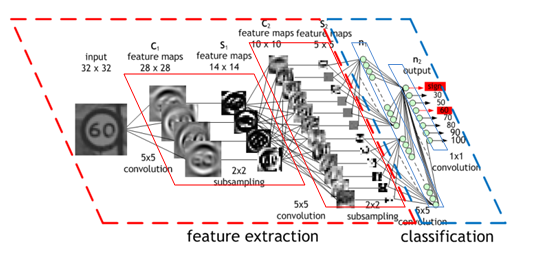
\includegraphics[scale=0.7]{convolutional_neural_network_structure} \]
  \centering
  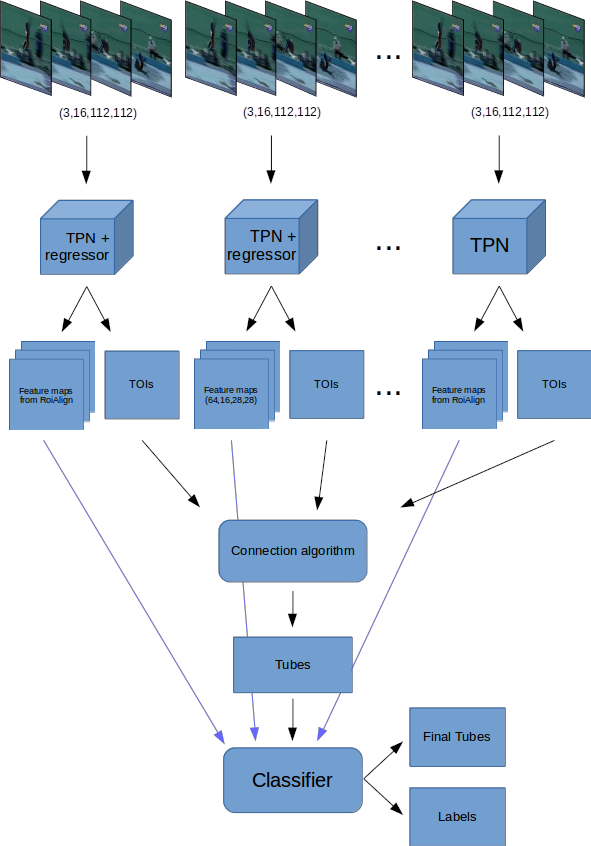
\includegraphics[scale=0.42]{model_prenms}
  \caption{\en Network's structure}
  \label{fig:gr_whole_network_}
\end{figure}
\gr
\section{\gr Εισαγωγή στο \tl{TPN}}
Ο κύριος σκοπός του  \en TPN  \gr  είναι να προτείνει \en\textbf{Tubes of Interest} (TOIs)\gr. Αυτά τα \en  tubes \gr  είναι πιθανό να περιέχουν μια γνωστή δράση και αποτελούνται από μερικά
δισδιάστατα πλαίσια (1 για κάθε καρέ βίντεο). Το \en  TPN \gr  είναι εμπνευσμένο από το \en  RPN \gr  που εισήχθη από το \en   FasterRCNN (\cite{Ren:2015:FRT:2969239.2969250})\gr ,
αλλά αντί για εικόνες, το \en  TPN \gr  χρησιμοποιείται σε βίντεο όπως κάνουν και οι \en \cite{DBLP:journals/corr/HouCS17}\gr . Σε πλήρη αντιστοιχία με τo \en  RPN \gr , η δομή
του \en  TPN \gr  είναι παρόμοια με αυτή  του \en  RPN\gr . Η μόνη διαφορά, είναι ότι το  \en TPN \gr  χρησιμοποιεί \en  3D Convolutional Layers  \gr και \en  3D anchors \gr  αντί  για \en  2D\gr.  \par
Σχεδιάσαμε 2 κύριες δομές για τo \en  TPN\gr. Κάθε προσέγγιση έχει διαφορετικό ορισμό για τα χρησιμοποιούμενα τρισδιάστατa \en  anchors\gr. 
Η υπόλοιπη δομή του \en  TPN \gr  είναι κυρίως η ίδια με ορισμένες μικρές διαφορές στο στάδιο του  \en  regression. \gr  \par

\section{Προετοιμασία πριν το \tl{TPN}}

\subsection{Η προετοιμασία των δεδομένων}
Πριν εισαχθεί ένα βίντεο στο  \en ResNet \gr  και στο \en  TPN \gr  για να εξαγάγουμε τα χαρακτηριστικά του και πιθανά \en  ToIs \gr , αυτό το βίντεο πρέπει να προεπερξαστεί.
Η διαδικασία προεπεξεργασίας είναι η ίδια και για τις δύο προσεγγίσεις του \en TPN\gr.
Η αρχιτεκτονική μας λαμβάνει ως είσοδο μια ακολουθία από σταθερό αριθμό καρέ  που έχουν σταθερό πλάτος και ύψος. Ωστόσο, κάθε βίντεο είναι πιθανόν να έχει διαφορετική ανάλυση. Αυτό δημιουργεί
την ανάγκη να αλλάξουμε  το μέγεθος κάθε καρέ και πλαισίου πριν εισαχθεί στο \en ActionNet\gr. Όπως αναφέρθηκε στο προηγούμενο κεφάλαιο, το πρώτο στοιχείο του δικτύου μας είναι ένα \en  3D RenNet  \gr
που υλοποιήθηκε από τους \en  \cite{hara3dcnns}\gr. Αυτό το δίκτυο έχει σχεδιαστεί να δέχεται βίντεο  με διαστάσεις (112, 112).
Ως αποτέλεσμα, μεταβάλλουμε  το μέγεθος κάθε καρέ από τα βίντεο των \en dataset \gr σε (112, 112). Για να διατηρήσουμε την αναλογία διαστάσεων, προσθέτουμε μηδενικές τιμές είτε
αριστερά και δεξιά, είτε πάνω και κάτω, ανάλογα με το ποια διάσταση είναι μεγαλύτερη. Στο σχήμα  \en\ref{fig:gr_Preprocess_example}\gr μπορούμε να δούμε το αρχικό καρέ καθώς και το αναδιαμορφωμένο.
Σε πλήρη αντιστοιχία, αλλάζουμε και το μέγεθος των πραγματικών πλαισίων οριοθέτησης για κάθε καρέ (Τα σχήματα
\en\ref{fig:gr_original_image_rois} \gr   και \en\ref{fig:gr_trans_image_rois} \gr  το απεικονίζουν).


\begin{figure}[h]
  \centering
  \begin{subfigure}{0.35\textwidth}
    \en
    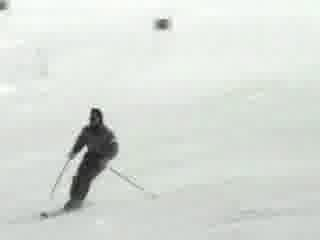
\includegraphics[width=\textwidth]{./figures/original_image.jpg}
    \caption{}
    \label{fig:gr_original_image}
   \end{subfigure}
  \hfill
  \begin{subfigure}{0.35\textwidth}
    \en
    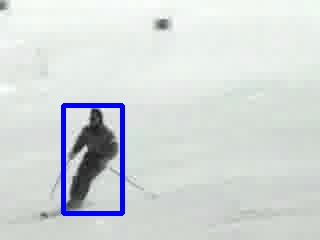
\includegraphics[width=\textwidth]{./figures/original_image_rois.jpg}
    \caption{}
    \label{fig:gr_original_image_rois}
  \end{subfigure}
  \hfill
  \begin{subfigure}{0.35\textwidth}
    \en
    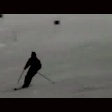
\includegraphics[width=\textwidth]{./figures/transformed_image.jpg}
    \caption{}
    \label{fig:gr_trans_image}
  \end{subfigure}
  \hfill
  \begin{subfigure}{0.35\textwidth}
    \en
    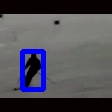
\includegraphics[width=\textwidth]{./figures/transformed_image_rois.jpg}
    \caption{}
    \label{fig:gr_trans_image_rois}
  \end{subfigure}

  \caption{\en At (a), (b) frame is its original size and at (c), (d) same frame after preprocessing part}
  \label{fig:gr_Preprocess_example}
\end{figure}


\subsection{\en 3D ResNet \gr}
Πριν από τη χρήση του \en Tube Proposal Network\gr, εξάγουμε  χωροχρονικά χαρακτηριστικά από το βίντεο. Για να γίνει αυτό, εξάγουμε τα 3 πρώτα στρώματα ενός
προεκπαιδευμένου \en 3D ResNet34\gr. Αυτό το μοντέλο είναι προεκπαιδευμένο στο \en Kinetics dataset (\cite{DBLP:journals/corr/KayCSZHVVGBNSZ17}\gr) για διάρκεια δείγματος ίση με
16 καρέ και μέγεθος δείγματος ίσο με (112, 122).  \par
Αυτό το δίκτυο συνήθως χρησιμοποιείται για την ταξινόμηση ολόκληρου του βίντεο, οπότε μερικά από τα στρώματα του χρησιμοποιούν \en temporal stride \gr ίσο με 2.
Εμείς, όμως, θέτουμε το \en temporal stride \gr ίσο με 1 γιατί δεν θέλουμε να χάσουμε χρονικές πληροφορίες κατά τη διάρκεια της διαδικασίας.
Έτσι, η έξοδος του τρίτου στρώματος είναι ένα χάρτης χαρακτηριστικών με διαστάσεις (256, 16, 7, 7). Τροφοδοτούμε αυτό τον χάρτη  χαρακτηριστικών στο \en TPN\gr,
το οποίο περιγράφεται στις ακόλουθες ενότητες.

\section{Τα τρισδιάστατα  \tl{anchors} ως  \tl{6-dim} διανύσματα}
\subsection{Πρώτη περιγραφή}
Ξεκινήσαμε να σχεδιάζουμε το \en TPN  \gr εμπνευσμένοι από την δουλειά των \en\cite{DBLP:journals/corr/HouCS17}\gr. Έτσι, θεωρούμε κάθε \en anchor \gr ως ένα
τρισδιάστατο πλαίσιο  το οποίο γράφεται ως \en $(x_1, y_1, t_1, x_2, y_2, t_2)$ \gr  όπου \en $x_1, y_1, t_1$ \gr  είναι
οι πάνω μπροστά αριστερές διαστάσεις του κύβου και \en $x_2, y_2, t_2$ \gr  είναι οι κάτω πίσω δεξιά όπως φαίνεται και στην εικόνα \ref{fig:gr_anchor_6d}.

\begin{figure}[h]
  \centering
  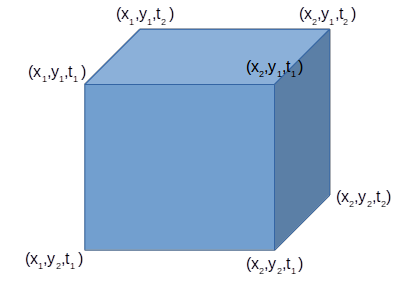
\includegraphics[scale=0.5]{anchor_6d}
  \caption{\en An example of the anchor $(x_1,y_1,t_1,x_2,y_2,t_2)$}
  \label{fig:gr_anchor_6d}
\end{figure}

Το κύριο πλεονέκτημα αυτής της προσέγγισης είναι ότι εκτός από τις διαστάσεις \en  x-y \gr , η διάσταση του χρόνου είναι μεταβαλλόμενη. Ως αποτέλεσμα, τα προτεινόμενα \en ToIs \gr
δεν έχουν καθορισμένη χρονική διάρκεια. Αυτό θα μας βοηθήσει να ασχοληθούμε με τα μη-κομμένα \en(untrimmed\gr) βίντεο, επειδή τα προτεινόμενα \en TOIs \gr  θα μπορούν να εξαιρέσουν \en background \gr
καρέ.
Για αυτήν την προσέγγιση, χρησιμοποιούμε \en\textbf{n = 4K = 60} anchors \gr  για κάθε \en  pixel \gr  στους χάρτες ενεργοποίησης του \en TPN\gr. Έχουμε \en k anchors \gr  για κάθε διαφορετική
  διάρκεια \en anchor \gr
 (5 κλίμακες των 1, 2, 4, 8, 16, 3 \en aspect rations 1:1, 1:2, 2:1\gr  και 4 διάρκειες 16, 12, 8 και 4 καρέ).
Σύμφωνα με τους \en\cite{DBLP:journals/corr/HouCS17}\gr,  τα \en anchors \gr  του δικτύου ορίζονται σύμφωνα με τα πιο συνηθισμένα \en anchors \gr  του συνόλου δεδομένων. Αυτό, ωστόσο,
δημιουργεί την ανάγκη επανασχεδιασμού του δικτύου για κάθε σύνολο δεδομένων. Στην προσέγγισή μας, χρησιμοποιούμε τα ίδια \en  anchors \gr  και για τα δύο σύνολα δεδομένων, επειδή θέλουμε το δίκτυό
μας να μην να βασίζεται στο σύνολο δεδομένων που του παρέχεται, αλλά να είναι σε θέση να γενικεύσει για διάφορα σύνολα δεδομένων. Ως διάρκεια δειγματοληψίας, επιλέξαμε 16 καρέ ανά τμήμα βίντεο, επειδή
η προ-εκπαιδευμένη έκδοση \en  ResNet \gr  που χρησιμοποιούμε έχει εκπαιδευτεί για βίντεο κλιπ με αυτή τη διάρκεια.
Έτσι, η δομή του \en  TPN \gr  είναι:
\begin{itemize}
\item\en 1 3D Convolutional Layer \gr με \en kernel size = 3, stride = 3 \gr  και \en padding = 1
\item\en 1 classification layer \gr  που εξάγει \en \textit{2n scores} \gr  για το αν υπάρχει ή όχι δράση για \en\textit{n tubes}.
\item\en 1 regression layer \gr  που εξάγει \textit{\tl{6n} διαστάσεις} \en ($x_1,y_1,t_1,x_2,y_2,t_2$) \gr  για \en\textit{n tubes}.
\end{itemize}

Η δομή του \en TPN \gr  παρουσιάζεται στην Εικόνα \ref{fig:gr_tpn_1_1}. Το αποτέλεσμα του \en  TPN \gr είναι τα \en   k\gr-καλύτερα κουτιά, τα οποία
είναι τα πιο πιθανά να περιέχουν κάποια δράση.

\en
\begin{figure}[h]
  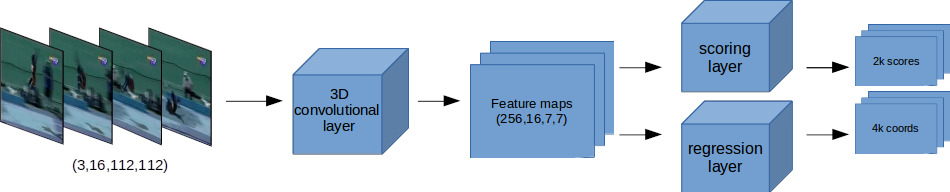
\includegraphics[width=1.\textwidth]{tpn_1_1}
  \caption{\en Structure of TPN}
  \label{fig:gr_tpn_1_1}
\end{figure}
\gr

\subsection{\tl{Training}}
\gr Όπως προαναφέρθηκε, το \en TPN \gr  εξάγει \en  ToIs \gr  ως 6-διάστατα διανύσματα. Για το λόγο αυτό, τροποποιήσαμε τα πραγματικά πλαίσια ανά καρέ σε πραγματικά \en  Tubes\gr.
Θεωρούμε δεδομένο ότι το άτομο που δρα, δεν μπορεί να κινηθεί πολύ σε 16 καρέ, γι' αυτό χρησιμοποιούμε τέτοιου είδους \en  Tubes \gr. Όπως φαίνεται 
στο σχήμα \ref{fig:gr_gt_tubes_and_rois}, αυτά τα \en tubes \gr είναι τρισδιάστατα κουτιά που περιλαμβάνουν όλα τα πραγματικά πλαίσια, τα οποία είναι διαφορετικά
ανά καρέ.


\begin{figure}[h]
  \centering
  \begin{subfigure}{0.15\textwidth}
    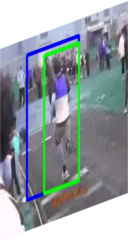
\includegraphics[width=\textwidth]{output/img_0.jpg}
  \end{subfigure}
  \begin{subfigure}{0.15\textwidth}
    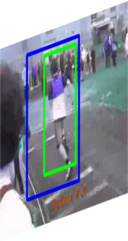
\includegraphics[width=\textwidth]{output/img_3.jpg}
  \end{subfigure}
  \begin{subfigure}{0.15\textwidth}
    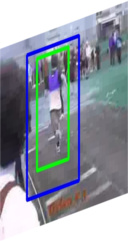
\includegraphics[width=\textwidth]{output/img_5.jpg}
  \end{subfigure}
  \begin{subfigure}{0.15\textwidth}
    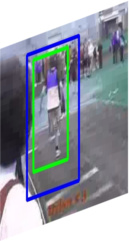
\includegraphics[width=\textwidth]{output/img_7.jpg}
  \end{subfigure}
  \begin{subfigure}{0.15\textwidth}
    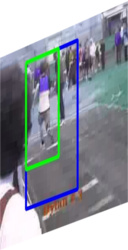
\includegraphics[width=\textwidth]{output/img_11.jpg}
  \end{subfigure}
  \begin{subfigure}{0.15\textwidth}
    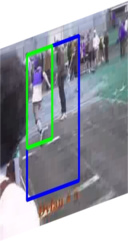
\includegraphics[width=\textwidth]{output/img_15.jpg}
  \end{subfigure}
  
  \caption{\en Groundtruth tube is colored with blue and groundtruth rois with color green}
  % \caption{\gr Το πραγματικό \en tube \gr έχει μπλε χρώμα και το πραγματικό ανά καρέ πλαίσιο έχει χρώμα πράσινο}
  \label{fig:gr_gt_tubes_and_rois}
\end{figure}


Για τη διαδικασία \en training\gr, για κάθε βίντεο, επιλέγουμε τυχαία ένα μέρος του, το οποίο έχει διάρκεια 16 καρέ. Θεωρούμε ένα \en anchor \gr ως πρώτο πλάνο,
αν η βαθμολογία επικάλυψης του με το πραγματικό
\en tube \gr είναι μεγαλύτερη από 0.5 . Διαφορετικά, θεωρείται ως \en anchor  \gr φόντου. Χρησιμοποιούμε έναν \en scoring layer \gr για να ταξινομήσουμε σωστά αυτά τα \en anchors \gr και χρησιμοποιούμε
την \en Cross Entropy Loss \gr ως συνάρτηση κόστους \en (loss function\gr). Έχουμε πολλά \en anchors \gr για να προτείνουμε μια δράση, αλλά μικρό αριθμό δράσεων σε κάθε βίντεο, έτσι επιλέγουμε \en
256 anchors \gr συνολικά για κάθε \en video\gr. Ορίζουμε ότι o μέγιστος αριθμός των \en anchors \gr προσκηνίου να είναι 25\% από τους 256 \en anchors \gr και τα υπόλοιπα είναι \en anchors \gr φόντου.  \par
Η σωστή ταξινόμηση ενός \en anchor \gr δεν είναι αρκετή για να προτείνουμε \en ToIs\gr. Είναι, επίσης,  απαραίτητο τα \en anchors \gr να επικαλύπτονται όσο το δυνατόν περισσότερο με τα πραγματικά \en
tubes\gr.
Αυτός είναι ο λόγος που χρησιμοποιούμε ένα επίπεδο παλινδρόμησης. Αυτό το \en layer \gr «κινεί» τον κύβο στην περιοχή που πιστεύεται ότι είναι πιο κοντά στη δράση.
Για συνάρτηση κόστους παλινδρόμησης χρησιμοποιούμε την συνάρτηση κόστους \en smooth-L1 \gr  όπως παρουσιάζεται από τους \en \cite{DBLP:journals/corr/GirshickDDM13}\gr. Για να υπολογίσουμε τους
 στόχους παλινδρόμησης, χρησιμοποιούμε την \en pytorch \gr εφαρμογή του  \en FasterRCNN (\cite{jjfaster2rcnn}\gr) για την παλινδρόμηση του πλαισίου και 
τροποποιούμε τον κώδικα επεκτείνοντας τον για 3 διαστάσεις. % Doobf{για περισσότερες πληροφορίες}
Έτσι έχουμε:
\en
\[ \begin{matrix}
    t_x = (x-x_a)/w_a, & t_y = (y-y_a)/h_a, & t_z= (z-z_a)/d_a, \\
    t_w= log(w/w_a), & t_h= log(h/h_a), & t_d = log(d/d_a), \\
    t^*_x = (x^* - x_a)/w_a, & t^*_y = (y^* - y_a)/h_a, & t^*_z = (z^* - z_a)/d_a, \\
    t^*_w = log(w^* /w_a), & t^*_h = log(h^*/h_a), & t^*_d = log(d^*/d_a),
    % t∗x= (x∗−xa)/wa,  t∗y= (y∗−ya)/ha,t∗w= log(w∗/wa),  t∗h= log(h∗/ha)
  \end{matrix}
\] \gr

όπου τα \en\textit{x, y, z, w, h, d} \gr υποδεικνύουν τις συντεταγμένες του κέντρου του τρισδιάστατου κουτιού καθώς επίσης το πλάτος, το ύψος και τη διάρκειά του. Οι μεταβλητές
\en $x, x_a, $\gr και \en $ x^*$ \gr αφορούν το προβλεπόμενο πλαίσιο, το πλαίσιο του \en anchor \gr και το πραγματικό πλαίσιο αντίστοιχα (ομοίως για \en \textit{y, z, w, h, d}\gr).
Φυσικά, υπολογίζουμε την απώλεια παλινδρόμησης μόνο για τα \en anchors \gr προσκηνίου και όχι αυτά του φόντου, συνεπώς στην χειρότερη θα υπολογίσουμε 64 στόχους για κάθε \en video.\gr \par

Για να συνοψίσουμε, στη διαδικασία \en training\gr, εκπαιδεύουμε 2 \en layers \gr για το \en TPN, \gr τα \en scoring \gr και \en reggression\gr. Η συνάρτηση κόστους περιλαμβάνει τα
\en training losses \gr που προκύπτουν απ' αυτά τα \en layers \gr και ο τύπος της είναι: \en
% \[ L  = \frac{1}{N_{cls}} \sum_iL_{cls}(p_i, p^*) + \frac{1}{N_{reg}}\sum_ip_i^*L_{reg}(t_i,t_i^*) \]
\[ L  =  \sum_iL_{cls}(p_i, p_i^*) + \sum_ip_i^*L_{reg}(t_i,t_i^*) \]
\gr όπου:
\begin{itemize}
\item \en $L_{cls} $ \gr είναι η \en Cross Entropy loss \gr που χρησιμοποιούμε γαι να εκπαιδεύσουμε τα \en anchors\gr, με \en $p_i$  \gr είναι η προβλεπόμενη κλάση, \en $p_i^*$ \gr
  είναι η πραγματική κλάση και \en   $p_i, p_i^* \in \{0,1\}$. \gr
\item \en $L_{reg} $ \gr είναι η συνάρτηση κόστους \en smooth-L1\gr, η οποία πολλαπλασιάζεται με \en $p_i^*$  \gr προκείμενου να ενεργοποιείται όταν υπάρχει θετικό \en anchor  $(p_i^* = 1)$ \gr
  και να απενεργοποιείται για τα \en background anchors $(p_i^* = 0)$.
\end{itemize}
\gr
\subsection{\tl{Validation}}

Η διαδικασία \en validation \gr είναι κάπως παρόμοια με τη διαδικασία του \en training\gr.
Επιλέγουμε τυχαία 16 καρέ από ένα βίντεο επικύρωσης, εξετάζουμε αν υπάρχει τουλάχιστον 1 προτεινόμενο \en ToI \gr
που επικαλύπτει $\ge$ 0,5 για κάθε πραγματικό \en tube  \gr και παίρνουμε το \en recall score\gr.
Για να λάβουμε καλές προτάσεις, μετά τη λήψη των \en classification scores \gr και των \en regression targets \gr από το
αντίστοιχα \en layers\gr, χρησιμοποιούμε τον αλγόριθμο \en Non-Maximum Suppresion(NMS)\gr.
Έχουμε ορίσει το κατώφλι του \en NMS \gr ίσο με 0,7 και κρατάμε τους πρώτους 150 κύβους με τη μεγαλύτερη βαθμολογία.
\subsection{\tl{Modified Intersection over Union(mIoU) } }
Κατά τη διάρκεια του \en training\gr, έχουμε πολλά \en anchors\gr. Πρέπει να τα ταξινομήσουμε ως \en anchors  \gr προσκηνίου ή
\en anchors \gr παρασκηνίου. Τα \en anchors \gr προσκηνίου είναι εκείνα που περιέχουν κάποια ενέργεια και, αντίστοιχα, του φόντου
που δεν έχουν. Tο \en IoU \gr για τα \en cuboids \gr υπολογίζει το ποσοστό μεταξύ του όγκου της επικάλυψης
και του όγκου των Ένωσης.
Διαισθητικά, αυτό το κριτήριο είναι καλό για την αξιολόγηση του βαθμού επικάλυψης 2 \en tube\gr, αλλά έχει ένα μεγάλο μειονέκτημα:
Θεωρεί ότι οι διαστάσεις \en x-y \gr έχουν την ίδια σημασία με τη χρονική διάσταση, τo οποίo δεν επιθυμούμε. Κι αυτό  διότι
πρώτον, μας ενδιαφέρει να είμαστε ακριβείς στη χρονική διάσταση, και στη συνέχεια μπορούμε να διορθώσουμε τον τομέα \en x-y\gr.
Ως αποτέλεσμα, αλλάζουμε τον τρόπο με τον οποίο υπολογίζουμε το \en Intersection over Union\gr. Υπολογίζουμε ξεχωριστά
το \en IoU \gr στις διαστάσεις \en x-y (IoU-xy) \gr και στην \en t \gr  διάσταση \en (IoU-t)\gr. Τέλος,  πολλαπλασιάζουμε αυτά τα δύο \en score
 \gr για να πάρουμε το τελικό \en IoU\gr.
Συνεπώς ο τύπος για 2 \en tubes ($x_1, y_1, t_1, x_2, y_2, t_2$) \gr  και \en  ($x'_1, y'_1, t'_1, x'_2, y'_2, t'_2$) \gr είναι:\en
\[ IoU_{xy} = \frac{ \text{Area of Overlap in x-y}} { \text{Area of Union in x-y}}  \]
\[ IoU_t = \frac { max(t_1, t'_1) - min(t_2, t'_2)} {min(t_1,t'_1) - max(t_2,t'_2)} \]
\[ IoU = IoU_{xy} \cdot  IoU_t \]
\gr Το παραπάνω κριτήριο μας βοηθά να εξισορροπήσουμε τις επιπτώσεις του χρόνου στο \en IoU score\gr. Για παράδειγμα, ας εξετάσουμε 2 \en anchors\gr:
\en a = (22, 41, 1, 34, 70, 5) \gr και \en  b = (20, 45, 2, 32, 72, 5)\gr. Αυτά τα 2 \en anchor \gr στις διαστάσεις \en  x-y \gr έχουν βαθμολογία \en IoU \gr ίσο με 0,61.
Αλλά δεν είναι ακριβώς επικαλυπτόμενα στην διάσταση του χρόνου. Χρησιμοποιώντας την πρώτη προσέγγιση έχουμε 0,5057 \en IoU \gr βαθμολογία ενώ η
δεύτερη προσέγγιση μας δίνει 0,4889. Έτσι, το δεύτερο κριτήριο θα απέρριπτε αυτό το \en  anchor\gr, διότι υπάρχει μια διαφορά στην χρονική διάρκεια. \par


Για να επιβεβαιώσουμε την ιδέα μας, εκπαιδεύουμε το \en TPN \gr χρησιμοποιώντας τόσο το \en IoU \gr κριτήριο όσο και το \en mIoU \gr  για την επικάλυψη των \en tubes\gr.
Στο πίνακα \ref{table:gr_iou_miou} μπορούμε να δούμε την απόδοση σε κάθε περίπτωση και για τα δύο σύνολα δεδομένων, \en JHMDB \gr και \en UCF\gr. Το \en recall \gr όριο για αυτή
την περίπτωση είναι 0,5 και κατά την διάρκεια του \en validation \gr χρησιμοποιούμε το κανονικό \en IoU \gr για να καθορίσουμε αν 2 \en tubes \gr επικαλύπτονται.

\en
\begin{table}[h]
  \centering
  \begin{tabular}{|| c | c || c ||}
    \hline
    \textbf{Dataset} & \textbf{Criterion} & \textbf{Recall(0.5)} \\
    \hline  \hline
    \multirow{2}{4em}{JHMDB} & IoU & 0.70525 \\
    \cline{2-3}
    {} & mIoU & 0.7052 \\
    \hline
    \multirow{2}{4em}{UCF} & IoU & 0.4665 \\
    \cline{2-3}
    {} & mIoU & 0.4829 \\
    \hline      
  \end{tabular}
  \caption{\en Recall results for both datasets using IoU and mIoU metrics}
  \label{table:gr_iou_miou}
\end{table}
\gr

Ο πίνακας  \ref{table:gr_iou_miou} μας δείχνει ότι το τροποποιημένο-\en IoU \gr μας δίνει ελαφρώς καλύτερη απόδοση \en recall \gr μόνο στο σύνολο δεδομένων \en UCF\gr.
Αυτό είναι λογικό, επειδή το σύνολο δεδομένων \en JHMDB \gr χρησιμοποιεί κομμένα βίντεο, συνεπώς  η χρονική διάρκεια δεν επηρεάζει πολύ. Έτσι, από τώρα και στο εξής,
κατά τη διάρκεια του \en training \gr χρησιμοποιούμε το \en mIoU  \gr ως επικαλυπτόμενη πολιτική βαθμολογίας.

\subsection{Βελτιώνοντας το  \tl{ TPN score}}
\gr Μετά την πρώτη δοκιμή, μας ήρθε η  ιδέα ότι σε ένα βίντεο που διαρκεί 16 καρέ, στην διάσταση του χρόνου, όλα τα είδη των ενεργειών μπορούν να χωρίζονται στις ακόλουθες κατηγορίες:
\begin{enumerate}
\item Η ενέργεια ξεκινά από το \tl{\textit{n}}-ο πλαίσιο και ολοκληρώνεται μετά το \textit{16o} καρέ του βίντεο που έχει υποβληθεί σε δειγματοληψία.
\item Η ενέργεια έχει ήδη ξεκινήσει πριν από το \textit{1o} καρέ του βίντεο και τελειώνει στο \tl{\textit{n}} πλαίσιο.
\item Η ενέργεια έχει ήδη ξεκινήσει πριν από το \textit{1o} καρέ του βίντεο και ολοκληρώνεται μετά το \textit{16o} καρέ βίντεο.
\item Η ενέργεια ξεκινά και τελειώνει σε αυτά τα 16 καρέ του βίντεο.
\end{enumerate}

Επιπλέον, παρατηρήσαμε ότι οι περισσότερες ενέργειες, στα σύνολα δεδομένων μας, διαρκούν περισσότερο από 16 καρέ. Έτσι, ήρθαμε με την ιδέα να προσθέσουμε 1 \en scoring layer \gr και 1
\en reggression Layer \gr που θα προτείνει \en ToIs  \gr με σταθερή διάρκεια ίση με τη διάρκεια του δείγματος (16 καρέ) και θα λάβει υπόψη τις χωρικές πληροφορίες που παράγονται
από τους χάρτες ενεργοποίησης. Η νέα δομή του \en TPN \gr εμφανίζεται στην εικόνα \ref{fig:gr_tpn_1_2}. Αφού λάβουμε τις προτάσεις και από και από τα δύο \en scoling layers\gr,
τις ενώνουμε με ποσοστό 1:1 μεταξύ των \en ToI \gr που εξαχθήκαν από τα δύο υποδίκτυα.

\en
\begin{figure}[h]
  \centering
  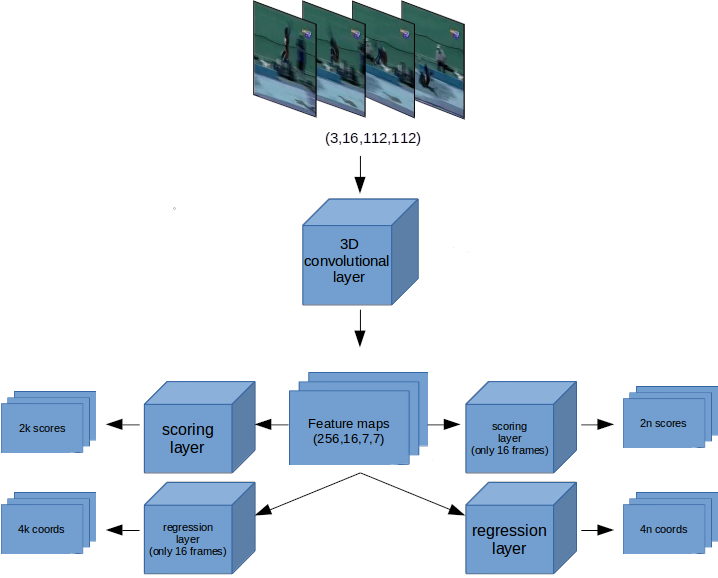
\includegraphics[scale=0.5]{tpn_1_2}
  \caption{\en TPN structure after adding 2 new layers, where k = 5n.}
  \label{fig:gr_tpn_1_2}
\end{figure}
\gr

Στόχος μας είναι να «συμπιέσουμε» τους χάρτες της χρονικής διάστασης, προκειμένου να προτείνουμε \en ToIs \gr σύμφωνα μόνο με τις χωρικές πληροφορίες.
Έτσι, βρίκαμε με 2 τεχνικές για να πραγματοποιήσουμε κάτι τέτοιο:
\begin{enumerate}
\item Να χρησιμοποιήσουμε \en  3D Convolutional Layers \gr με μέγεθος πυρήνα = διάρκεια δείγματος, 1, 1), \en stride \gr = 1 και χωρίς \en padding \gr για \en scoring \gr και \en regression\gr.
  Αυτός ο πυρήνας «κοιτάει» μόνο στη χρονική διάσταση των χαρτών ενεργοποίησης και δεν θεωρεί καμία χωρική εξάρτηση.
\item Nα υπολογίσουμε τις μέσες τιμές από τη χρονική διάσταση και στη συνέχεια να χρησιμοποιήσουμε ένα \en 2D Convolutional Layer \gr για \en scoring \gr και \en regression\gr.
\end{enumerate}

% \textbf{TODO na perigrapsw oti thelw na exw ola ta xronika features}
\par
Οι διαδικασίες \en training \gr και \en validation \gr παραμένουν ίδιες. Η μόνη μεγάλη διαφορά είναι ότι τώρα έχουμε κόστη  από 2  συστήματα που προτείνουν \en TOIs\gr.
Παράλληλα, κατα την διάρκεια του \en validation\gr, εμείς αρχικά, ενώνουμε τα προτεινόμενα \en ToIs \gr και, στη συνέχεια, ακολουθούμε την ίδια διαδικασία, η οποία είναι να
υπολογίσουμε το \en recall\gr. Για το \en training loss\gr, έχουμε 2 διαφορετικές \en Cross-entropy losses \gr συναρτήσεις και 2 διαφορετικά \en smooth-L1 losses\gr. Έτσι,
η απώλεια εκπαίδευσης, τώρα, ορίζεται ως:

  % \begin{aligned}
 % L  =  \sum_iL_{cls}(p_i, p_i^*) + \sum_iL_{cls}(p_{fixed,i}, p_{fixed,i}^*) +  
 %  \sum_ip_i^*L_{reg}(t_i,t_i^*) + \sum_ip_{fixed,i}^*L_{reg}(t_{fixed,i},t_{fixed,i}^*) 
% L  =2


% \[ L  =  \sum_iL_{cls}(p_i, p_i^*) + \sum_iL_{cls}(p_{fixed,i}, p_{fixed,i}^*) +  \newline
%   \sum_ip_i^*L_{reg}(t_i,t_i^*) + \sum_ip_{fixed,i}^*L_{reg}(t_{fixed,i},t_{fixed,i}^*) \]
% \end{aligned}

\en
\begin{equation} 
\begin{split}
 L  =  \sum_iL_{cls}(p_i, p_i^*) + \sum_iL_{cls}(p_{fixed,i}, p_{fixed,i}^*) + \\
   \sum_ip_i^*L_{reg}(t_i,t_i^*) + \sum_ip_{fixed,i}^*L_{reg}(t_{fixed,i},t_{fixed,i}^*) 
  % \sum_iL_{cls}(p_i, p_i^*) + \sum_iL_{cls}(p_{fixed,i}, p_{fixed,i}^*) 
\end{split}
\end{equation}
\gr

όπου:
\begin{itemize}
\item\en $L_{cls} $ \grείναι η \en Cross Entropy loss \gr που χρησιμοποιούμε για να εκπαιδεύσουμε τα \en anchors\gr, με \en $p_i$ \gr είναι η προβλεπόμενη κλάση, \en $p_i^*$ \gr είναι
  η πραγματική κλάση και   \en $p_i, p_i^* \in \{0,1\}$
\item\en $L_{reg} $ \gr είναι η συνάρτηση κόστους \en smooth-L1\gr, η οποία πολλαπλασιάζεται με \en $p_i^*$ \gr προκείμενου να ενεργοποιείται όταν υπάρχει θετικό \en anchor $(p_i^* = 1)$ \gr
  και να απενεργοποιείται για τα \en background anchors $(p_i^* = 0)$.
\item\en $p_i $ \gr είναι τα \en anchors \gr από τα \en scoring \gr και \en regression layers \gr με μεταβλητή χρονική διάρκεια και  \en $p_i^*$ \gr είναι η αντίστοιχη πραγρατική τους κλάση.
\item\en $p_{fixed,i} $ \gr είναι τα \en anchors \gr από τα \en scoring \gr και \en regression layers \gr με σταθερή χρονική διάρκεια ίση με 16 καρέ και \en $p_{fixed,i}^*$  \grείναι η
  αντίστοιχη πραγματική του κλάση.

\end{itemize}

Εκπαιδεύουμε το δίκτυο \en TPN \gr χρησιμοποιώντας και τις δύο τεχνικές και η  απόδοση του \en recall \gr εμφανίζεται στον πίνακα  \ref{table:gr_add_16}.

\en
\begin{table}[h]
  \centering
  \begin{tabular}{||c | c | c || c ||}
    \hline
    \textbf{Dataset} & \textbf{Fix-time anchors} & \textbf{Type} & \textbf{Recall(0.5)} \\
    \hline  \hline
    \multirow{3}{4em}{JHMDB} & No &  - & 0.7052 \\
    \cline{2-4}
    {} & \multirow{2}{*}{Yes} & Kernel & 0.6978 \\
    \cline{3-4}
    {} & {} & Mean & 0.7463 \\
    \hline
    \multirow{3}{4em}{UCF} & No & - & 0.4829 \\
    \cline{2-4}
    {} & \multirow{2}{*}{Yes} & Kernel & 0.4716 \\
    \cline{3-4}
    {} & {} & Mean & 0.4885 \\
    \hline      
  \end{tabular}
  \caption{\en Recall results after adding fixed time duration anchors}
  \label{table:gr_add_16}
\end{table}
\gr

Όπως μπορούμε να δούμε από τα προηγούμενα αποτελέσματα, τα νέα \en layers \gr αύξησαν σημαντικά την απόδοση του \en recall\gr. Πέρα από αυτό, ο πίνακας \ref{table:gr_add_16} δείχνει ότι
η λήψη των μέσων τιμών από τη χρονική διάσταση μας δίνει τα καλύτερα αποτελέσματα.


\subsection{Προσθήκη \tl{Regressor}}
Το αποτέλεσμα του \en TPN  \gr είναι τα $\alpha$-υψηλότερα βαθμολογικά \en anchors \gr που μετακινήθηκαν σύμφωνα με την \en regression \gr πρόβλεψη τους. Μετά από αυτό, πρέπει να μετατρέψουμε τα
προτεινόμενα \en anchors \gr σε \en ToIs\gr.
Για να γίνει αυτό, προσθέτουμε ένα σύστημα παλινδρόμησης που παίρνει ως είσoδο τους χάρτες χαρακτηριστικών των τρισδιάστατων κουτιών και επιστρέφει μια ακολουθία από δισδιάσταστα κουτιά,
ένα για κάθε καρέ.
Το μόνο πρόβλημα είναι ότι η παλινδρόμηση χρειάζεται ως είσοδο χάρτες χαρακτηριστικών  σταθερού μεγέθους. Αυτό το πρόβλημα είναι ήδη λυμένο από τα \en R-CNNs  \gr που χρησιμοποιούν \en ROI pooling \gr
και \en ROI align \gr προκειμένου να λάβουν σταθερού μεγέθους χάρτες ενεργοποίησης από \en ROIs \gr μεταβαλλόμενου μεγέθους. Στην περίπτωση μας, επεκτείνουμε την λειτουργία \en RoI Align\gr ,
που παρουσιάζεται από το \en MaskR-CNN(\cite{DBLP:journals/corr/HeGDG17})\gr, και εμείς το ονομάζουμε \en\textbf{3D ROI align}.
\paragraph{3D Roi Align}
\en To  \en 3D ROI align \gr είναι μια τροποποίηση του \en ROI Align \gr που παρουσιάστηκε από τo \en MaskR-CNN\gr. Η κύρια διαφορά μεταξύ αυτών των δύο είναι ότι το
\en MaskR-CNN\gr, στο \en RoiAlign\gr,  χρησιμοποιεί διγραμμική παρεμβολή για την εξαγωγή των χαρακτηριστικών των \en ROIs \gr και το δικός μας \en 3D ROI Align \gr χρησιμοποιεί
τριγραμμική παρεμβολή για τον ίδιο λόγο. Και πάλι, η 3η διάσταση είναι χρόνος.
Συνεπώς, έχουμε ως είσοδο ένα χάρτη χαρακτηριστικών που εξάγεται από το \en  ResNet34  \gr με διαστάσεις (64, 16, 28, 28) και έναν τένσορα που περιέχει τα προτεινόμενα \en ToIs\gr.
Για κάθε \en ToI \gr του οποίου ο χάρτης ενεργοποίησης έχει μέγεθος ίσο με (64, 16, 7, 7), έχουμε ως έξοδο ένα χάρτη χαρακτηριστικών με μέγεθος (64, 16, 7, 7).  \par

\subsubsection{\en Regression procedure}
\gr Στην αρχή, για κάθε προτεινόμενο \en ToI\gr, έχουμε τους αντίστοιχους χάρτες ενεργοποίησης χρησιμοποιώντας \en 3D ROI align\gr. Αυτά τα χαρακτηριστικά δίνονται ως είσοδο σε έναν \en Regressor\gr.
Αυτός επιστρέφει 16 $\cdot$ 4 προβλεπόμενες μεταβολές $(\delta_x,\delta_y, \delta_w,\delta_h)$, 4 για κάθε καρέ, όπου $ \delta_x, \delta_y$ καθορίζουν τις συντεταγμένες του κέντρου των προτάσεων και
$\delta_w, \delta_h$ το πλάτος και το ύψος του, όπως ορίζεται από τους \en\cite{DBLP:journals/corr/GirshickDDM13}\gr.
Κρατάμε μόνο τις προβλεπόμενες μεταβολές, για τα καρέ που $\ge t_1$ και $< t_2$ και για υπόλοιπα θέτουμε ένα μηδενικό \en 2D \gr κουτί. 
Μετά από αυτό, τροποποιούμε κάθε \en anchor\gr, γραμμένο ως έναν κύβο δηλαδή γραμμένο ως $(x_1,y_1,t_1, x_2, y_2, t_2)$ σε μια ακολουθία πλαισίων \en 2D\gr, όπως: \\
$(0,0,0,0, ..., x_{T_1},y_{T_1},x'_{T_1},y'_{T_1}, ... ,x_{i},y_{i},x'_{i}, ..., x_{T_2},y_{T_2},x'_{T_2},y'_{T_2}, 0,0,0,0, ....)$, \\
όπου:
\begin{itemize}
\item $ T_1 \le i \le T_2$, για $T_1 < t_1 + 1,  T_2 < t_2 \text{ και }T_1,T_2 \in \mathbb{Z} $
\item $ x_i = x_1, y_i= y_1, x'_i = x_2, y'_i = y_2 $.
\end{itemize}

\paragraph{\tl{ Training}}
Για να εκπαιδεύσουμε τον \en Regressor \gr μας, ακολουθούμε τα ίδια βήματα που ακολουθήσαμε προηγουμένως για την προηγούμενη διαδικασία εκπαίδευσης του \en TPN\gr. Αυτό σημαίνει ότι 
επιλέγουμε τυχαία 16  \en ToIs \gr από αυτές που προτείνονται από το \en scoring layer \gr του \en TPN\gr. Απ' αυτά, 4 είναι τα \en anchors \gr προσκηνίου, το οποίο σημαίνει ότι αποτελούν το 25\%
του συνολικού αριθμoύ των \en anchors \gr όπως συνέβη προηγουμένως. Εξάγουμε τα αντίστοιχα χαρακτηριστικά τους χρησιμοποιώντας \en 3D ROI Algin \gr και υπολογίζουμε τους στόχους τους, όπως
κάναμε για το \en regression layer\gr. Τροφοδοτούμε το δίκτυο μας με αυτά τα χαρακτηριστικά και συγκρίνουμε τους προβλεπόμενους στόχους με τούς αναμενόμενους.
Ξανά πάλι, χρησιμοποιούμε \en smooth-L1 loss function \gr για τη συνάρτηση κόστους, υπολογίζoντας την μόνο για \en ToIs \gr που είναι στο προσκήνιο. Έτσι, προσθέτουμε μια άλλη παράμετρο στο
φόρμουλα απώλειας εκπαίδευσης που πλέον ορίζεται ως:
\en
\begin{equation} 
\begin{split}
 L  =  \sum_iL_{cls}(p_i, p_i^*) + \sum_iL_{cls}(p_{fixed,i}, p_{fixed,i}^*) + \\
 \sum_ip_i^*L_{reg}(t_i,t_i^*) + \sum_ip_{fixed,i}^*L_{reg}(t_{fixed,i},t_{fixed,i}^*) + \\
  \sum_iq_i^*L_{reg}(c_{i}, c_{i}^*) + \\
  % \sum_iL_{cls}(p_i, p_i^*) + \sum_iL_{cls}(p_{fixed,i}, p_{fixed,i}^*) 
\end{split}
\end{equation}
\gr όπου εκτός από τις παραμέτρους που καθορίστηκαν προηγουμένως, ορίζουμε $c_{i} $ ως στόχους παλινδρόμησης για τα επιλεγμένα \en tubes \gr $q _I $.
Αυτά τα \en tubes \gr είναι που επιλέγονται τυχαία από τα προτεινόμενα \en ToIs \gr και  $q_i^*$ είναι τα αντίστοιχοι πραγματικά \en tubes\gr, τα οποία είναι τα  πλησιέστερα σε κάθε $q_i$ \en tube\gr.
Και πάλι χρησιμοποιούμε το $q_i^*$ ως παράγοντα, επειδή θεωρούμε ένα \en tube \gr ως φόντο όταν δεν επικαλύπτεται με οποιοδήποτε πραγματικό \en tube \gr περισσότερο από 0,5.

\paragraph{\tl{Validation}}
Χρησιμοποιούμε, ξανά, τη μετρική \en recall \gr για να αξιολογήσουμε την απόδοση τoυ παλινδρομητή. Υπολογίζουμε 3 επιδόσεις \en recall\gr:
\begin{description}
\item [\tl{Cuboid Recall},] που είναι η \en recall \gr μετρική για τα προτεινόμενα τρισδιάστατα κουτιά. Ενδιαφερόμαστε για αυτήν την επίδοση γιατί,
  θέλουμε να μάθουμε πόσο καλές είναι οι προτάσεις μας πριν τις τροποποιήσουμε σε σειρές κουτιών.
\item [\tl{Single frame Recall},] η οποία είναι η επίδοση \en recall \gr για τις προτεινόμενες ακολουθίες κουτιών σε σχέση με τις πραγματικές.
\item[\tl{Follow-up Single Frame Recall},] που είναι η απόδοση της ανάκλησης μόνο για τα τρισδιάστατα Κουτιά που ήταν πάνω από το όριο επικάλυψης μεταξύ
  των προτεινόμενων κύβων και των πραγματικών κύβων. Χρησιμοποιούμε αυτή τη μετρική για να γνωρίζουμε πόσα από τους προτεινόμενα τρισδιάστατα κουτιά
  κατέληξαν να είναι καλές προτάσεις.
\end{description}


\subsubsection{Αρχιτεκτονικές για τον \en Regressor \gr} 
Σχεδιάσαμε 2 προσεγγίσεις για την υλοποίηση του \en Regressor\gr. Aυτές απεικονίζονται στις Εικόνες \ref{fig:gr_regressor_3d} και \ref{fig:gr_reg_1_2}, με την πρώτη προσέγγιση
να αποτελείται από ένα \en 3D Convolutional Layer \gr σε αντίθεση με την δεύτερη προσέγγιση που έχει ένα \en 2D Convolutional Layer\gr.

\en
\begin{figure}[h]
  \centering
  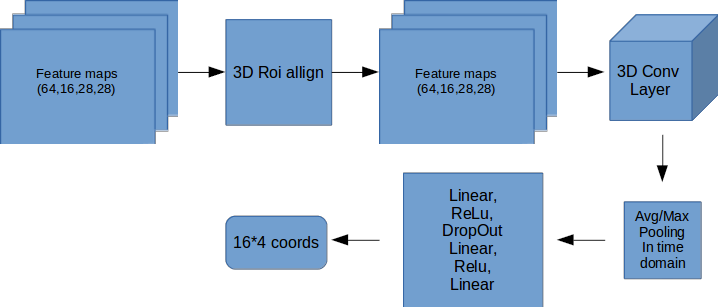
\includegraphics[scale=0.48]{regressor_1_1}
  \caption{\en Structure of Regressor}
  \label{fig:gr_regressor_3d}
\end{figure}
\gr
\en
\begin{figure}[h]
  \en
  \centering
  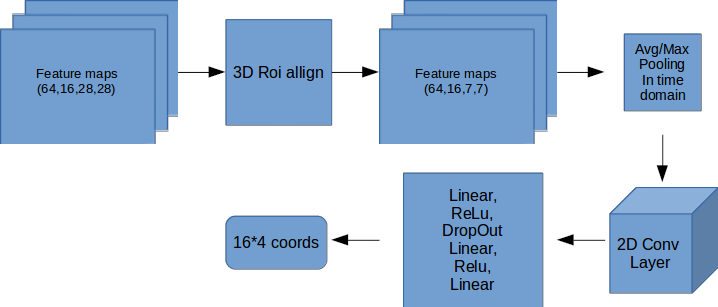
\includegraphics[scale=0.48]{regressor_1_2}
  \caption{\en Structure of Regressor}
  \label{fig:gr_reg_1_2}
\end{figure}
\gr

Η διαδικασία που ακολουθούν και οι δύο \en Regressors \gr περιγράφεται παρακάτω:
\begin{enumerate}
\item Αρχικά εξάγουμε τα αντίστοιχα \en feature maps \gr για κάθε \en ToI \gr χρησιμοποιώντας \en 3D Roi Align\gr, και ακολούθως τα κανονικοποιούμε. Μετά, στην πρώτη προσέγγιση
τροφοδοτούμε ένα \en 3D Convolutional Layer \gr με \en  kernel \gr ίσο με 1, \en stride \gr ίσο με 1 και χωρίς \en padding\gr. Στην συνέχεια, εφαρμόζουμε μια
\en pooling \grδιαδικασία στην διάσταση του χρόνου (είτε \en avg \gr είτε \en max pooling\gr). Απ'   την άλλη, στην δεύτερη προσέγγιση, πρώτα εφαρμόζουμε \en avg/max pooling \gr στην
διάσταση του χρόνου και στην συνέχεια τροφοδοτούμε ένα \en 2D Convolutional Layer \gr με \en kernel = 1, stride = 1 \gr και χωρίς \en padding\gr.
\item Και στις δύο περιπτώσεις λαμβάνουμε ως έξοδο ένα \en feature map \gr με διαστάσεις (64,7,7) το οποίο περνάμε διαδοχικά από 1 γραμμικό  \en layer, 1 Relu Layer, 1 Dropout Layer, \gr
  άλλο ένα γραμμικό \en Layer\gr, άλλο ένα \en ReLu layer \gr και ένα τελικό γραμμικό \en layer\gr. Το τελευταίο \en layer \gr μας δίνει ως έξοδο 64 στόχους, 4 $\cdot$ 16 μετακινήσεις.
\end{enumerate}

\en
\begin{table}[h]
  \en
  \centering
  \begin{tabular} {||c | c || c | c | c ||}
    \hline
    \textbf{Dataset} & \textbf{Pooling} & \textbf{Cuboid} & \textbf{Singl. Fr. } &  \textbf{Follow-up S.F.}\\
    \hline                
    \multirow{2}{*}{JHMDB} & avg & 0.8545 & 0.7649 & 0.7183 \\
    \cline{2-5}
    {} & max & 0.8396 & 0.7761 & 0.5783 \\
    \cline{1-5}
    \multirow{2}{*}{UCF} & avg & 0.5319 & 0.4694 & 0.5754 \\
    \cline{2-5}
    {} & max & 0.5190 & 0.5021 & 0.5972 \\
    \cline{1-5}
                                   
  \end{tabular}
  \caption{\en Recall results after convertying cuboids into sequences of frames}
  \label{table:gr_reg_1_1}
\end{table}
\gr
\en
\begin{table}[h]
  \en
  \centering
  \begin{tabular}{||c | c | c || c  c  c ||}
    \hline
    \textbf{Dataset} & \textbf{Pooling} & \textbf{F. Map} & \textbf{Recall} &  \textbf{ Recall SR}  &  \textbf{Recall SRF} \\
    \hline
    \multirow{6}{*}{JHMDB} & \multirow{3}{*}{mean} & 64 &  0.6828  & 0.5112  & 0.7610 \\
    \cline{3-6}
    {} & {} & 128 & 0.8694 & 0.7799 & 0.6756 \\
    \cline{3-6}
    {} & {} & 256 & 0.8396 & 0.7687 & 0.7029 \\
    \cline{2-6}
    {} & \multirow{3}{*}{max} & 64 &  0.8582 & 0.7985 & 0.5914\\
    \cline{3-6}
    {} & {} & 128 & 0.8358 & 0.7724 & 0.8118 \\
    \cline{3-6}
    {} & {} & 256 & 0.8657 & 0.8022 & 0.7996 \\
    \hline
    \multirow{6}{*}{UCF} & \multirow{3}{*}{mean} & 64 & 0.5055 & 0.4286 & 0.5889 \\
    \cline{3-6}
    {} & {} & 128 & 0.5335 & 0.4894 & 0.5893 \\
    \cline{3-6}
    {} & {} & 256 & 0.5304 & 0.4990 & 0.6012 \\
    \cline{2-6}
    {} & \multirow{3}{*}{max} & 64 & 0.5186 & 0.4990 & 0.5708 \\
    \cline{3-6}
    {} & {} & 128 & 0.5260 & 0.4693 & 0.5513 \\
    \cline{3-6}
    {} & {} & 256 & 0.5176 & 0.4878 & 0.6399 \\
    \hline

  \end{tabular}
  \caption{\en Recall performance using 3 different feature maps as Regressor's input and 2 pooling methods}
  \label{table:gr_reg_1_2}
\end{table}
\gr
Οι πίνακες \ref{table:gr_reg_1_1} και \ref{table:gr_reg_1_2} περιέχουν τα αποτελέσματα για την πρώτη και δεύτερη προσέγγιση. Μάλιστα, για την δεύτερη προσέγγιση ελέγξαμε 3 διαφορετικούς χάρτες
χαρακτηριστικών, ενώ και στις 2 περιπτώσεις πειραματιστήκαμε χρησιμοποιώντας και τις 2 προαναφερθέντες \en pooling \gr μεθόδους για τα σύνολα δεδομένων \en JHMDB \gr και \en UCF-101\gr.
Παρατηρούμε ότι, με βάση τα παραπάνω αποτελέσματα, λαμβάνουμε σχετικά χαμηλή \en recall \gr απόδοση για το \en dataset UCF \gr ενώ για το \en JHMDB \gr  τα αποτελέσματα είναι κάπως καλύτερα.
Πιο συγκεκριμένα, με βάση την πρώτη προσέγγιση λαμβάνουμε τελικά \en recall \gr απόδοση ίση με 76-77\% για το \en JHMDB \gr και 46-50\% για το \en UCF\gr. Με βάση την δεύτερη προσέγγιση,
στην καλύτερη περίπτωση λαμβάνουμε 80\% απόδοση \en recall  \gr για το \en JHMDB \gr ενώ για το \en UCF \gr παραμένουμε στα ίδια περίπου αποτελέσματα.
Παράλληλα παρατηρούμε ότι χάνουμε περίπου 30-40\% από τις καλές \en cuboid \gr προτάσεις και στις 2 περιπτώσεις, το οποίο αποτελεί μεγάλο πρόβλημα και των δύο προσεγγίσεων.
Όλ' αυτά μας κάνουν να ξανασκεφτούμε τον τρόπο που σχεδιάσαμε το \en TPN \gr και μας οδήγησε στο να σχεδιάσουμε ένα νέο μοντέλο.


\section{Τα τρισδιάστατα \tl{anchors} ως \tl{4k} διανύσματα}
Σε αυτή την προσέγγιση, ορίζουμε τους \en 3D anchors \gr ως διανύσματα με \en 4k \gr συντεταγμένες (\tl{k} = 16 καρέ = διάρκεια δείγματος).
Έτσι ένα τυπικό \en anchor \gr γράφεται ως ($x_1, y_1, x'_1, y'_1, x_2, y_2, ...$)
όπου $x_1, y_1, x'_1, y'_1 $ είναι οι συντεταγμένες για 1ο καρέ, $x_2, y_2, x'_2, y'_2$ για το 2ο καρέ κλπ, όπως παρουσιάστηκε από τους \en\cite{DBLP:journals/corr/abs-1712-09184}\gr. 
Η εικόνα \ref{fig:gr_anchor_4k} απεικονίζει ένα τέτοιου τύπου \en anchor\gr.

\en
\begin{figure}[h]
  \centering
  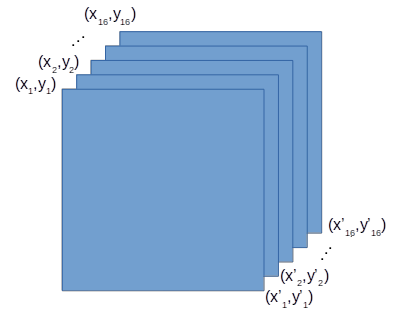
\includegraphics[scale=0.5]{anchor_4k}
  \caption{An example of the anchor $(x_1,y_1,x'_1,y'_1,x_2,y_2, ...)$}
  \label{fig:gr_anchor_4k}
\end{figure}
\gr

Το κύριο πλεονέκτημα αυτής της προσέγγισης είναι ότι δεν χρειάζεται να μεταφράσουμε τα \en 3D anchors \gr σε δισδιάστατα κουτιά, γεγονός που προκάλεσε πολλά προβλήματα στην προηγούμενη προσέγγιση.
Ωστόσο, αυτή η προσέγγιση έχει ένα μεγάλο μειονέκτημα, το οποίο είναι το γεγονός ότι αυτός ο τύπος \en anchor \gr έχει σταθερή χρονική διάρκεια.
Για να αντιμετωπίσουμε αυτό το πρόβλημα, έχουμε ορίσει \en anchors \gr με διαφορετικές χρονικές διάρκειες, οι οποίες είναι 16, 12, 8 και 4 καρέ.
\en Anchors \gr με διάρκεια $<$  διάρκεια του δείγματος (16 καρέ) μπορούν  να γραφτούν ως διάνυσμα \en 4k \gr με μηδενικές συντεταγμένες στα καρέ μεγαλύτερα από τη χρονική διάρκεια.
Για παράδειγμα, ένα \en anchor \gr με 2 καρέ διάρκεια, ξεκινώντας από το 2ο καρέ και τερματίζοντας στον 3ο μπορεί να γραφεί ως
(0, 0, 0, 0, $x_1, y_1, x'_1, y'_1, x_2, y_2, x'_2, y'_2$, 0, 0, 0, 0)  εάν η διάρκεια δείγματος
είναι 4 καρέ. 

\en
\begin{figure}[h]
  \centering
  % 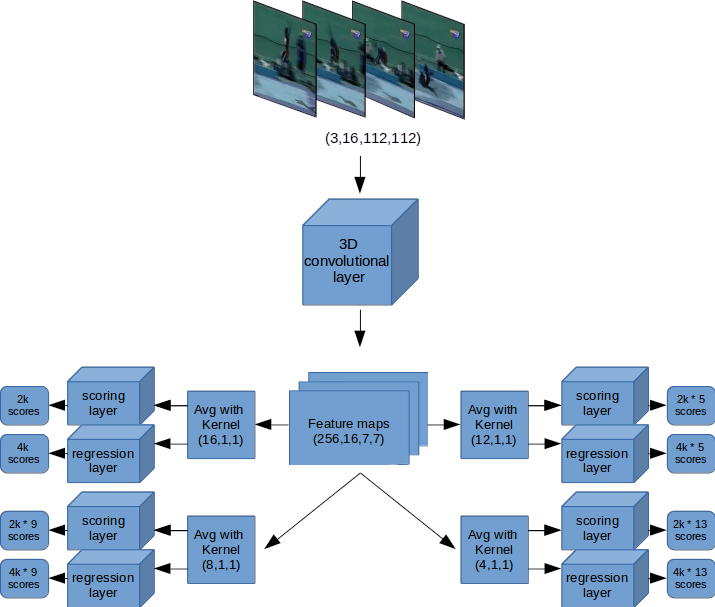
\includegraphics[width=1.\textwidth]{tpn_2}
  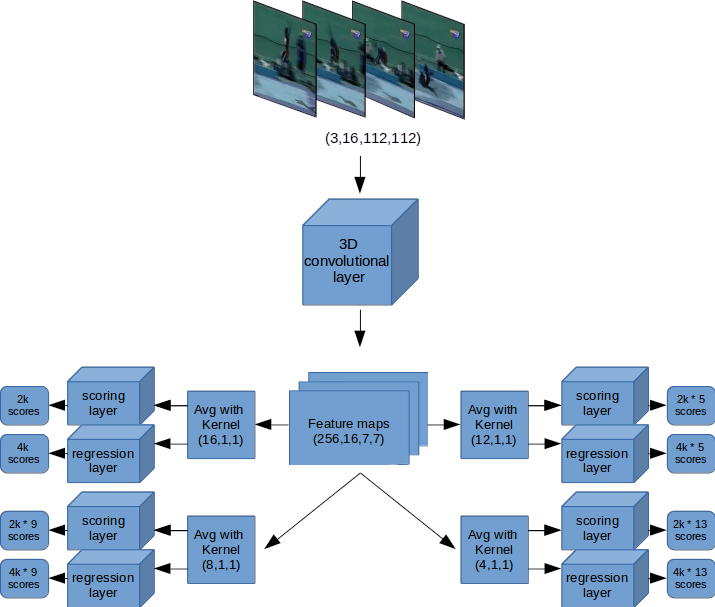
\includegraphics[scale=0.4]{tpn_2}
  \caption{\en The structure of TPN according to new approach}
  \label{fig:gr_New_structure}
\end{figure}

\gr

Αυτή η νέα προσέγγιση μας οδήγησε στο να αλλάξουμε την δομή του \en TPN\gr. Η νέο δομή του απεικονίζεται στην εικόνα  \ref{fig:gr_New_structure}. Όπως
μπορούμε να δούμε, προσθέσαμε \en scoring \gr και \en regression layers \gr για κάθε διάρκεια. Έτσι, το \en TPN \gr ακολουθεί τα επόμενα βήματα για να παράγει \en ToIs\gr.
\begin{enumerate}
\item Στην αρχή, τροφοδοτούμε τον χάρτη χαρακτηριστικών, που εξάγεται από το \en 3D ResNet34\gr, ως είσοδο σε ένα \en 3D Convolutional Layer \gr με μέγεθος πυρήνα = 1,
  \en stride = 1 \gr και χωρίς \en padding\gr.
\item Από το \en Convolutional Layer\gr, έχουμε ως έξοδο ένα χάρτη ενεργοποίησης με διαστάσεις (256, 16, 7, 7). Για τη μείωση της χρονικής διάστασης, χρησιμοποιούμε 4 \en pooling layers\gr,
  ένα για κάθε δείγμα διάρκειας με μεγέθη πυρήνα  \textit{(16, 1, 1), (12, 1, 1,), (8, 1, 1) και (4, 1, 1)} και \en stride = 1\gr, για τη διάρκεια του δείγματος 16, 12, 8 και 4 καρέ αντίστοιχα.
  Έτσι, έχουμε χάρτες ενεργοποίησης με διαστάσεις \textit{(256, 1, 7, 7), (256, 5, 7, 7), (256, 9, 7, 7) και (256, 13, 7, 7)}, στης oποίες η δεύτερη διάσταση είναι ο αριθμός των πιθανών
  χρονικών διακυμάνσεων. Για παράδειγμα, σε  χάρτη χαρακτηριστικών με διαστάσεις $(256, 5, 7, 7)$, το οποίο σχετίζεται με \en anchors \gr με διάρκεια 12 καρέ, μπορούμε να έχουμε 5 πιθανές περιπτώσεις,
  από το καρέ 0 μέχρι το καρέ 11, από το καρέ 1 μέχρι το καρέ 12 κλπ.
  
\item Ξανά, όπως και στην προηγούμενη προσέγγιση, για κάθε \en pixel \gr του χάρτη ενεργοποίησης αντιστοιχούμε \en\textbf{n = k = 15}
  anchors \gr(5 κλίμακες από 1, 2, 4, 8, 16, και 3 \en aspect ratios \gr 1:1, 1:2, 2:1). Φυσικά, έχουμε 4 διαφορετικούς χάρτες ενεργοποίησης, με 1, 5, 9 και 13
  διαφορετικές περιπτώσεις και  $7  \times 7$ διαστάσεις σε κάθε φίλτρο. Έτσι, συνολικά έχουμε $28  \cdot 15 \cdot 49 = 20580$ διαφορετικά \en anchors\gr.
  Αντίστοιχα, έχουμε 20580 διαφορετικούς στόχους \en regression\gr.

\end{enumerate}

\subsection{\tl{Training}}
Η διαδικασία \en training \gr παραμένει σχεδόν η ίδια όπως και στην προηγούμενη προσέγγιση. Έτσι, και πάλι, εμείς τυχαία επιλέγουμε ένα τμήμα βίντεο και τα αντίστοιχα πραγματικά \en tubes\gr. Όμως,
θεωρούμε τα \en anchors \gr ως προσκήνιο όταν έχουν επικάλυψη  μεγαλύτερη από 0,8 με οποιαδήποτε πραγματικό \en tube\gr, ενώ θεωρούμε \en anchors \gr παρασκηνίου αυτά  των οποίων η επικάλυψη
είναι μεγαλύτερη που 0,1 και μικρότερη από 0,3. Δεν ασχολούμαστε με τα υπόλοιπα \en anchors\gr. 

\en
\begin{table}[h]
  \centering
  \begin{tabular}{||c | c || c  c c||}
    \hline
    \textbf{Dataset} & \textbf{Pooling} &  \textbf{Recall(0.5)} & \textbf{Recall(0.4)} & \textbf{Recall(0.3)} \\
    \hline  \hline
    \multirow{2}{4em}{JHMDB} & mean & 0.6866 & 0.7687 & 0.8582 \\
    \cline{2-5}
    {} & max &  0.8134 & 0.8694 & 0.9216 \\
    \hline
    \multirow{2}{4em}{UCF} & avg &  0.5435 & 0.6326 & 0.7075 \\
    \cline{2-5}
    {} & max & 0.6418 & 0.7255 & 0.7898 \\
    \hline
  \end{tabular}
  \caption{\en Recall results using 2nd approach for anchors}
  \label{table:gr_tpn_2_1}
\end{table}
\gr


Όπως δείχνει ο πίνακας \ref{table:gr_tpn_2_1}, είναι προφανές ότι έχουμε καλύτερες επιδόσεις \en recall \gr σε σύγκριση με την προηγούμενη προσέγγιση.
Επιπλέον, μπορούμε να δούμε ότι το \en 3D max pooling \gr  αποδίδει καλύτερα από το \en 3D avg pooling\gr. Η διαφορά
μεταξύ των δύο είναι περίπου 10\%, η οποία είναι αρκετά μεγάλη για να μας κάνει να επιλέξουμε το \en max pooling \gr ως λειτουργία ομαδοποίησης πριν από τη
λήψη των \en scores \gr και \en regression targets \gr των \en anchors\gr.

\subsection{Προσθήκη \tl{Regressor}}

Ακόμα και αν, το  \en TPN \gr μας εξάγει κουτιά σε επίπεδο καρέ, πρέπει να βελτιώσουμε αυτές τις προβλέψεις προκειμένου να αλληλοεπικαλύπτονται
με τα πραγματικά κουτιά  όσο το δυνατόν καλύτερα.
Έτσι, σε πλήρη αντιστοιχία με την προηγούμενη προσέγγιση, προσθέσαμε έναν \en Regressor \gr για να προσπαθήσουμε να πάρουμε καλύτερα αποτελέσματα \en recall\gr.

\paragraph{\tl{3D Roi align}}
Σε αυτή την προσέγγιση, γνωρίζουμε ήδη τις χωρικές συντεταγμένες. Έτσι, μπορούμε να χρησιμοποιήσουμε τη μέθοδο που προτείνεται από τους \en\cite{DBLP:journals/corr/abs-1712-09184}\gr. Αποτελεί
επέκταση του \en RoiAlign \gr χωρίζοντας το \en tube \gr σε $T$ δισδιάστατα κουτιά. Στη συνέχεια, χρησιμοποιείται το  κλασικό \en RoiAlign \gr για να εξαχθεί  μια περιοχή από κάθε μίας από τα 
χρονικά \en slices \gr στον χάρτη ενεργοποίησης. Μετά από αυτό, τα \en feature maps \gr που προέκυψαν μέσω του \en RoiAlign \gr συνδέονται στην διάσταση του χρόνου, ώστε να προκύψει
χάρτης χαρακτηριστικών με διαστάσεις $T \times R \times R$,  όπου $R $ είναι η ανάλυση εξόδου του \en RoiAlign\gr, το οποίο είναι 7 στην περίπτωσή μας.  \par


Εκπαιδεύουμε τον \en Regressor \gr μας χρησιμοποιώντας την ίδια \en loss function \gr όπως ο τύπος της προηγούμενης προσέγγισης που είναι:
\begin{equation*} 
\begin{split}
 L  =  \sum_iL_{cls}(p_i, p_i^*) + \sum_iL_{cls}(p_{fixed,i}, p_{fixed,i}^*) + \\
 \sum_ip_i^*L_{reg}(t_i,t_i^*) + \sum_ip_{fixed,i}^*L_{reg}(t_{fixed,i},t_{fixed,i}^*) + \\
  \sum_iq_i^*L_{reg}(c_{i}, c_{i}^*) + \\
  % \sum_iL_{cls}(p_i, p_i^*) + \sum_iL_{cls}(p_{fixed,i}, p_{fixed,i}^*) 
\end{split}
\end{equation*}

Και σ' αυτήν την προσέγγιση χρησιμοποιούμε 2 διαφορετικές αρχιτεκτονικές για την υλοποίηση του \en Regressor\gr.
Ως πρώτη προσέγγιση, χρησιμοποιούμε ένα \en 3D Convolutional Layer \gr ακολουθούμενο από 2 γραμμικά \en Layer\gr. Aντίστοιχα, στην δεύτερη προσέγγιση χρησιμοποιούμε ένα \en 2D
Convolution Layer \gr ακολουθούμενο, και αυτό, από 2 γραμμικά \en Layer\gr. H πρώτη προσέγγιση είναι ακριβώς η ίδια με πριν. Ωστόσο, η δεύτερη προσέγγιση
αντιμετωπίζει τα \en feature maps \gr σαν να μην υπάρχουν χρονικές εξαρτήσεις μεταξύ τους. Δηλαδή:
\begin{enumerate}
\item Στην αρχή, χρησιμοποιούμε το \en 3D Roi Align \gr για να εξάγουμε τα \en feature maps \gr Και μετά τα κανονικοποιούμε. Έστω λοιπόν ότι προκύπτουν \tl{k} χάρτες ενεργοποιήσης
  με διαστάσεις (\tl{k}, 256, 16, 7, 7)
\item Χωρίζουμε τα υποψήφια \en ToIs \gr σε \en T 2D \gr κουτιά, οπότε οι διαστάσεις του τένσορα που περιέχει τις συντεταγμένες των \en ToIs \gr γίνονται από $(k,4\cdot sample duration)$
  σε $(k,sample duration, 4)$. Διαφοροποιούμε τον τένσορα ώστε να πάρει τις διαστάσεις  $(k\cdot sample duration, 4)$, όπου οι πρώτες \tl{k} συντεταγμένες αναφέρονται
  στο πρώτο καρέ, οι επόμενες \tl{k} στο δεύτερο κλπ.
\item Αντίστοιχα διαφοροποιούμε και τους χάρτες ενεργοποίησης όπου από διαστάσεις $(k, 64, sample duration, 7, 7)$ καταλήγουμε σε χάρτες με διαστάσεις $(k\cdot sample duration, 64, 7, 7)$.
  Πλέον λοιπόν επεξεργαζόμαστε του χάρτες χαρακτηριστικών σαν να είναι δισδιάστατοι. Έτσι τροφοδοτούμε το \en 2D Convolutional Layer \gr και ακολουθούμενο από τα άλλα δύο γραμμικά \en Layer\gr.
  \item Τα εξαγόμενα \en targets\gr, φυσικά θα είναι μόνο 4 όσο δηλαδή για 1 καρέ.
\end{enumerate}

\en
\begin{table}[h]
  \centering
  \begin{tabular}{||c | c || c  c  c||}
    \hline
    \textbf{Dataset} & \textbf{Feat. Map} & \textbf{Recall(0.5)} & \textbf{Recall(0.4)} & \textbf{Recall(0.3)}\\
    \hline
    \multirow{2}{*}{JHMDB} &  64 & 0.7985 & 0.903 & 0.9552 \\
    \cline{2-5}
    {} & 128 & 0.7836 & 0.8881 & 0.944\\
    \hline
    \multirow{2}{*}{UCF}  & 64 & 0.5794 & 0.7206 & 0.8134 \\
    \cline{2-5}
    {} & 128 & 0.5622 & 0.7204 & 0.799 \\
    \hline

  \end{tabular}
  \caption{Recall performance when using a 3D Convolutional Layer in Regressor's architecture}
  \label{table:gr_reg_2_1}
\end{table}
\gr
\en

\begin{table}[h]
  \centering
  \begin{tabular}{||c | c || c  c  c||}
    \hline
    \textbf{Dataset}  & \textbf{Feat. Map} & \textbf{Recall(0.5)} & \textbf{Recall(0.4)} & \textbf{Recall(0.3)}\\
    \hline
    \multirow{3}{*}{JHMDB} & 64 & 0.8358 & 0.9216 & 0.9739\\
    \cline{2-5}
    {} & 128 & 0.8172 & 0.9142 & 0.9627 \\
    \cline{2-5}
    {} & 256 & 0.7724 & 0.8731 & 0.9328 \\
    \hline
    \multirow{3}{*}{UCF} & 64 & 0.6368 & 0.7346 & 0.7737 \\ 
    \cline{2-5}
    {} & 128 & 0.6363 & 0.7133 & 0.7822 \\
    \cline{2-5}
    {} & 256 &  0.6363 & 0.7295 & 0.7822 \\
    \hline

  \end{tabular}
  \caption{Recall performance when using a 2D Convolutional Layer instead of 3D in Regressor's model}
  \label{table:gr_reg_2_2}
\end{table}
\gr

Με βάση τους παραπάνω πίνακες \en\ref{table:gr_reg_2_1}\gr και \en\ref{table:gr_reg_2_2}\gr, η καλύτερη επίδοση προκύπτει για τους χάρτες χαρακτηριστικών μεγέθους $(64,16,7,7)$. Αυτό το
αποτέλεσμα ήταν αναμενόμενο γιατί αυτοί οι χάρτες ενεργοποίησης βρίσκονται «πιο κοντά» στα πραγματικά χαρακτηριστικά. Συγκρίνοντας
τις δύο προτεινόμενες μεθόδους παρατηρούμε ότι η δεύτερη, αυτή δηλαδή που χρησιμοποιεί \en 2D Convolutional Layer \gr έχει τα καλύτερα
αποτελέσματα. Αν και βελτιώσαμε την απόδοση του \en TPN \gr ακόμα δεν έχουμε καταφέρει να έχουμε σχεδόν σε όλες τις περιπτώσεις
καλές προτάσεις \en tube\gr.
\subsection{Μείωση της διάρκειας του δείγματος}
Προκειμένου να πετύχουμε καλύτερα αποτελέσματα αποφασίσαμε να μειώσουμε την διάρκεια του δείγματος από τα 16 καρέ σε 8 και 4 αντίστοιχα. Κι
αυτό γιατί με αυτόν τον τρόπο θα μειωθούν παράλληλα με τον αριθμός τους οι διαστάσεις των \en anchors, \gr  άρα και οι διαστάσεις των στόχων παλινδρόμησης και γενικά ο αριθμός των παραμέτρων που πρέπει να εκπαιδευτούν από το σύστημα. \par
Εκπαιδεύουμε το \en TPN \gr με και χωρίς \en Regressor \gr προκειμένου να βρούμε την κατάλληλη αρχιτεκτονική. Τα αποτελέσματα χωρίς \en Regressor \gr
παρουσιάζονται στον πίνακα \ref{table:gr_new_sample} ενώ τα αποτελέσματα της αρχιτεκτονικής με \en Regressor \gr στον πίνακα \ref{table:gr_new_sample_reg}.

\en
\begin{table}[h]
  \centering
  \begin{tabular}{|c | c || c c c|}
    \hline
    \textbf{Dataset} & \textbf{Sample dur} & \textbf{Recall(0.5)} &  \textbf{Recall(0.4)} &  \textbf{Recall(0.3)} \\
    \hline
    \multirow{3}{*}{JHMDB} & 16 & 0.8134 & 0.8694 & 0.9216 \\
    \cline{2-5}
    {} & 8 & 0.9515 & 0.9888 & 1.0000 \\
    \cline{2-5}
    {} & 4 & 0.8843 & 0.9627 & 0.9888 \\
    \hline
    \multirow{3}{*}{UCF} & 16 & 0.6418 & 0.7255 & 0.7898 \\
    \cline{2-5}
    {} & 8 & 0.7942 & 0.8877 & 0.9324\\
    \cline{2-5}
    {} & 4 & 0.7879 & 0.8924 & 0.9462 \\
    \hline
    
  \end{tabular}
  \caption{\en Recall results when reducing sample duration to 4 and 8 frames per video segment}
  \label{table:gr_new_sample}
\end{table}
\gr
\en
\begin{table}[h]
  \centering
  \begin{tabular}{|c | c | c || c c c|}

    \hline
    \textbf{Dataset} & \textbf{Sample dur} & \textbf{Type} & \textbf{Recall(0.5)} &  \textbf{Recall(0.4)} &  \textbf{Recall(0.3)} \\
    \hline
    \multirow{4}{*}{UCF} & \multirow{2}{*}{8} & 2D & 0.8078 & 0.8870 & 0.9419 \\
    \cline{3-6}
    {} & {} & 3D & 0.8193 & 0.8930 & 0.9487 \\
    \cline{2-6}
    {} & \multirow{2}{*}{4}& 2D & 0.7785 & 0.8914 & 0.9457 \\
    \cline{3-6}
    {} & {} & 3D & 0.7449 & 0.8605 & 0.9362 \\
    \hline
    \multirow{4}{*}{JHDMBD} & \multirow{2}{*}{8} & 2D &  0.9366 & 0.9851 & 0.9925  \\
    \cline{3-6}
    {} & {} & 3D & 0.8918 & 0.9776 & 0.9963  \\ 
    \cline{2-6}
    {} & \multirow{2}{*}{4}& 2D & 0.9552 & 0.9963 & 1.0000 \\
    \cline{3-6}
    {} & {} & 3D & 0.9142 & 0.9701 & 0.9888  \\
    \hline
    
  \end{tabular}
  \caption{\en Recall results when a regressor and sample duration equal with 4 or 8 frames per video segment}
  \label{table:gr_new_sample_reg}

\end{table}
\gr

Το πρώτο συμπέρασμα που προκύπτει από τους πίνακες \ref{table:gr_new_sample} και  \ref{table:gr_new_sample_reg}  είναι ότι όντως μειώνοντας την
διάρκεια του δείγματος πετυχαίνουμε καλύτερα αποτελέσματα. Παράλληλα, με βάση τον πίνακα \ref{table:gr_new_sample_reg} και δεδομένων των
προηγούμενων αποτελεσμάτων (Πίνακες \ref{table:gr_reg_2_1} και \ref{table:gr_reg_2_2}) γίνεται ξεκάθαρο ότι η προσέγγιση που περιλαμβάνει
ένα \en 2D Convolutional Layer \gr υπερέχει αυτής με το \en 3D Convolutional Layer\gr. Σ' οτι αφορά τα σύνολα δεδομένων παρατηρούμε ότι
η προσέγγιση με διάρκεια δείγματος 8 καρέ υπερέχει σχεδόν σε όλες τις περιπτώσεις. Συνεπώς, για τα επόμενα κεφάλαια θα προτιμάται
να χρησιμοποιείται αυτή.

% \end{document}
\documentclass{report}

\usepackage[ english, greek]{babel}
\usepackage[utf8]{inputenc}
\usepackage[LGR, T1]{fontenc}

% % 

\newcommand{\tl}{\textlatin}
\newcommand{\en}{\selectlanguage{english}}
\newcommand{\gr}{\selectlanguage{greek}}

\usepackage{hyperref}  % package for linking figures etc
\usepackage{enumitem}  % package for description with bullets
\usepackage{graphicx}  % package for importing images
\usepackage{mathtools} % package for math equation
\usepackage{mathrsfs}  % package for math font
\usepackage{indentfirst} % package for getting ident after section or paragraph
\usepackage{subcaption} % package for subfigures
\usepackage[export]{adjustbox}
\usepackage{longtable} % package for multi pages tables
\usepackage{multirow}  % package for tables, multirow
\usepackage{amssymb}
\usepackage{esvect}
\usepackage[
backend=bibtex,
citestyle=authoryear,
% citestyle=authoryear-comp,
% citestyle=authoryear-ibid,
bibstyle=numeric,
sorting=ynt,
% style=numeric,
% style=alphabetic ,
]{biblatex}
\addbibresource{References}

\graphicspath{ {./theory/figures/} }       % path for images

\begin{document}
\gr 
 
\chapter{Αλγόριθμος σύνδεσης των \en action tubes\gr}

Στο προηγούμενο κεφάλαιο περιγράψαμε μεθόδους για την παραγωγή υποψήφιων \en ToIs\gr, δεδομένου ενός μικρού τμήματος βίντεο που διαρκεί 8 ή 16 καρέ. Ωστόσο, τα πραγματικά βίντεο και πραγματικές ανθρώπινες ενέργειες, σε εξωτερικές συνθήκες, διαρκούν πάνω από 16 καρέ τις περισσότερες φορές. Τα τρέχοντα δίκτυα δεν είναι σε θέση να επεξεργαστούν ένα ολόκληρο βίντεο με την μία, προκειμένου να προτείνει υποψήφια \en ToIs\gr,
λόγω προβλημάτων μνήμης και υπολογιστικής ενέργειας.
Πολλές προσεγγίσεις για εντοπισμό δράσης λύνουν αυτό το πρόβλημα, δεδομένου ενός βίντεο, είτε
προτείνουν υποψήφιες περιοχές σε επίπεδο καρέ και, στη συνέχεια, τις συνδέουν με σκοπό τη δημιουργία υποψήφιων \en action tubes\gr, είτε
το διαχωρίζουν σε τμήματα βίντεο, προτείνοντας ακολουθίες από δυσδιάστα πλαίσια τα οποία στην συνέχεια συνδέουν για να δημιουρηγήσουν
\en action proposals\gr.
Και οι δύο προαναφερθείσες προσεγγίσεις καθιστούν την κατάλληλη επιλογή της μεθόδου σύνδεσης σημαντικό παράγοντα για την απόδοση του δικτύου.
Αυτό συμβαίνει επειδή, παρόλο που στο επίπεδο καρέ ή στο επίπεδο τμήματος βίντεο
οι προτάσεις μπορεί να είναι πολύ καλές, αν ο προτεινόμενος αλγόριθμος σύνδεσης δεν λειτουργεί καλά, οι τελικές προτάσεις \en action tubes \gr
δεν θα είναι αποτελεσματικές, οπότε το τελικό μοντέλο δεν θα
είναι σε θέση να επιτύχει υψηλή απόδοση ταξινόμησης.
Με άλλα λόγια, αν ο αλγόριθμος σύνδεσης δεν δημιουργεί προτάσεις δράσης με μεγάλο \en recall \gr και καλή απόδοση \en MABO\gr,
ο ταξινομητής του μοντέλου δεν θα είναι σε θέση να εκτελέσει την κατάλληλη ταξινόμηση, επειδή πιθανώς θα του έχουν δοθεί \en action tubes \gr χωρίς κανένα περιεχόμενο.
Σε αυτό το κεφάλαιο, παρουσιάζουμε 3 διαφορετικές προσεγγίσεις που χρησιμοποιούνται για τη σύνδεση των προτεινόμενων ToIs που παράγονται από το \en TPN \gr του προηγούμενου κεφαλαίου.

\section{Πρώτη προσέγγιση: συνδυασμός επικάλυψης και πιθανότας δράσης}
Ο αλγόριθμος μας εμπνέεται από την προσέγγιση των \en\cite{DBLP:journals/corr/HouCS17}\gr, η οποία υπολογίζει όλες τις πιθανές ακολουθίες των \en ToIs\gr. Για να βρει τα  καλύτερα υποψηφία \en action tubes\gr,
χρησιμοποιεί μια βαθμολογία που μας λέει πόσο πιθανό μια ακολουθία του TOIs είναι να περιέχει μια ενέργεια. Αυτή η βαθμολογία είναι ένας συνδυασμός 2 μετρικών:
\begin{description}
\item[ Πιθανότητα δράσης ή Δραστικότητα(\tl{Actioness}), ] που είναι η πιθανότητα ενός \en ToI \gr να περιέχει μια δράση. Αυτό το σκορ
  παράγεται από τα \en scoring layers \gr  του \en TPN\gr.
\item [Σκορ επικάλυψης μεταξύ των \en ToIs\gr, ] το οποίο είναι το \en IoU \gr των τελευταίων πλασίων του πρώτου \en ToI \gr και των πρώτων πλαισίων του δεύτερου \en ToIs\gr.
\end{description}

Η παραπάνω πολιτική βαθμολόγησης μπορεί να περιγραφεί από τον ακόλουθο τύπο:

\[ S = \frac{1}{m} \sum_ {i=1}^{m} Actioness_i + \frac{1}{m-1} \sum_{j=1}^{m-1} Overlap_{j,j+1} \]

Για κάθε πιθανό συνδυασμό \en ToIs\gr, υπολογίζουμε το σκορ του όπως φαίνεται στην εικόνα \ref{fig:connection_algo}.

\begin{figure}[h]
  \centering
  \en
  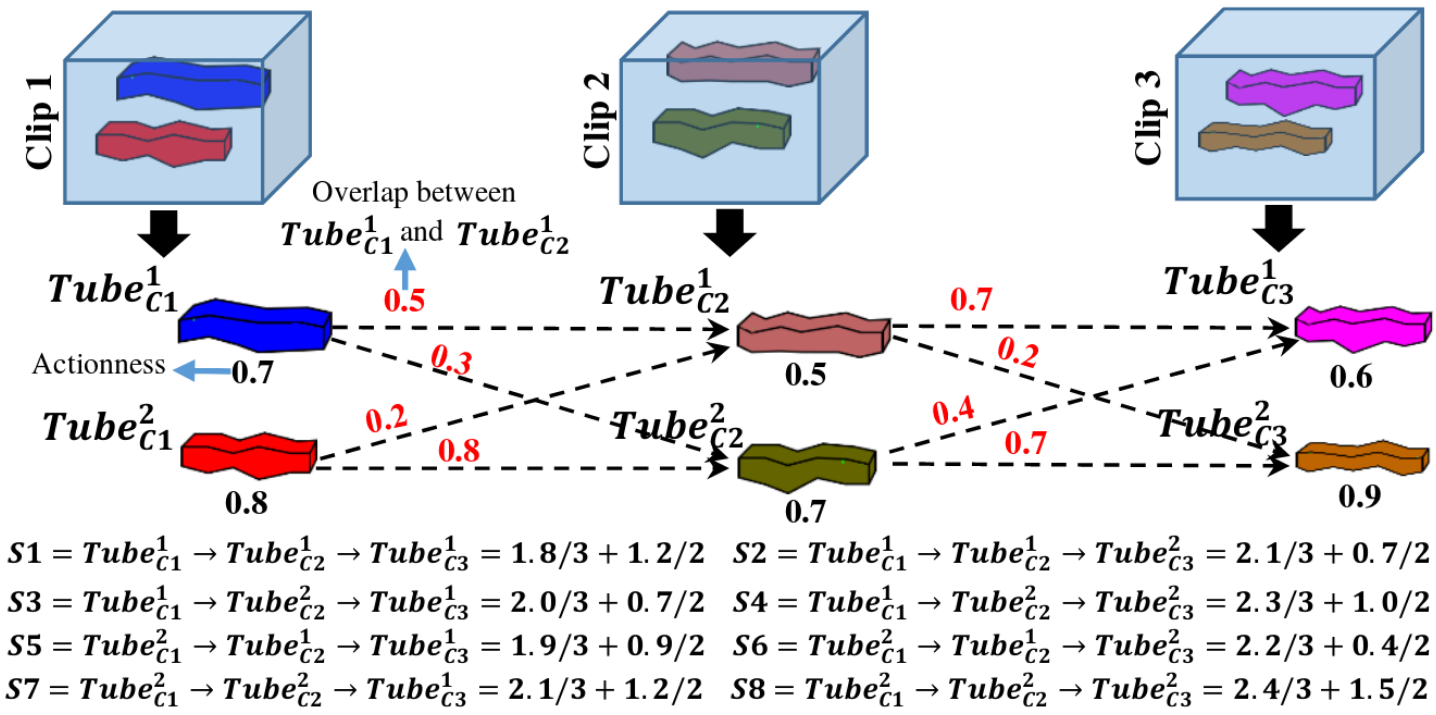
\includegraphics[scale=0.225]{connection_algo}
  \caption{An example of calculating connection score for 3 random TOIs taken from \cite{DBLP:journals/corr/HouCS17}}
  \label{fig:connection_algo}
\end{figure}

Η παραπάνω προσέγγιση, όμως, χρειάζεται υπερβολικά πολύ μνήμη για την πραγματοποίηση όλων αυτών των υπολογισμων, έτσι
ένα πρόβλημα μνήμης εμφανίζεται. Ο λόγος έιναι πως για κάθε νέο βίντεο κλιπ, εμείς προτείνουμε \en\textit{k ToIs} (\gr 16
κατά την διάρκεια της εκπαίδευσης και 150 κατά την διάρκεια του \en validation\gr.
Σαν αποτέλεσμα, για ένα μικρό βίντεο χωρισμένο σε \textbf{10 }μέρη, χρειάζεται να υπολογίσουμε
\textbf{$150^{10}$} σκορ κατά την διάρκεια της επικύρωσης. Αυτό οδηγεί το σύστημα μας να χρειάζεται υπερβολικά πολύ χρόνο
για να το πραγματοποιήσει.

Για να αντιμετωπίσουμε αυτό το πρόβλημα, δημιουργούμε έναν άπληστο αλγόριθμο για να βρούμε τα υποψήφια \en action tubes\gr.
Ο αλγόριθμος αυτός, για κάθε νέο τμήμα βίντεο, κρατά τα \en tubes \gr με βαθμολογία υψηλότερη από ένα κατώφλι και διαγράφει τα υπόλοιπα.
Έτσι, δεν χρειάζεται να υπολογίσουμε συνδυασμούς με πολύ χαμηλό σκορ. Γράψαμε κώδικα για τον υπολογισμό των βαθμολογιών των \en tubes \gr
στη γλώσσα \en CUDA\gr, η οποία έχει ως δυνατότητα την παράλληλη επεξεργασία του ίδιου κώδικα χρησιμοποιώντας διαφορετικά δεδομένα. Ο αλγόριθμος μας περιγράφεται παρακάτω:

\begin{enumerate}
\item Πρώτον, αρχικοποιούμε  κενές λίστες για τα τελικά \en tubes\gr,την διάρκεια τους, τις βαθμολογίες τους, τα ενεργά \en tubes\gr,
  τη διάρκειά τους, το άθροισμα των σκορ επικάλυψης  και δραστηκότητας τους όταν:
  \begin{itemize}
  \item Η λίστα με τα τελικά \en tubes \gr περιέχει όλα τα \en tubes  \gr που είναι πιθανότερο να περιέχουν μια ενέργεια και η λίστα
    βαθμολογίας τους περιέχει τις αντίστοιχες βαθμολογίες τους. Αναφερόμαστε σε κάθε \en tube \gr από τον δείκτη του, ο οποίος
    σχετίζεται με ένα τένσορα, στον οποίο σώσαμε όλα τα \en ToIs \gr που προτείνονται από το \en TPN \gr για κάθε τμήμα βίντεο.
  \item Η λίστα ενεργών \en tubes \gr περιέχει όλα τα \en tubes \gr που θα συνδιαστούν με τα νέα \en  TOIs\gr.
    Η  λίστα άθροισης των επικαλυπτώμενων σκορ  και η λίστα άθροισης δραστικότητας περιέχουν τα αντίστοιχα αθροίσματα τους,
    προκειμένου να αποφεύγεται ο υπολογισμός τους για κάθε βρόχο. 
  \end{itemize}
Επίσης, προετοιμάζουμε το όριο σύνδεσης ίσο με 0,5.
\item Για το πρώτο τμήμα βίντεο, προσθέτουμε όλα τα \en ToIs \gr τόσο στα ενεργά \en tubes \gr όσο και στα τελικά \en tubes\gr.
  Οι βαθμολογίες τους είναι μόνο η δική τους δραστηκότητας επειδή δεν υπάρχουν \en tubes \gr για τον υπολογισμό της μεταξύ τους
  επικαλυπτόμενης βαθμολογίας. Έτσι, έτσι ορίζουμε το άθροισμα επικάλυψης ίσο με 0.
\item Για κάθε επόμενο βίντεο, μετά την λήψη των προτεινόμενων \en ToIs\gr, πρώτα υπολογίζουμε το σκορ επικάλυψης τους με κάθε
  ενεργό \en tube\gr. Μετά, αδειάζουμε την λίστα με τα ενεργά \en tubes\gr, με την διάρκεια τους, το άθροισμα επικάλυψης και το
  άθροισμα πιθανοτήτων δράσης. Για κάθε νέο \en tube \gr που έχει βαθμολογία υψηλότερη από το κατώφλι σύνδεσης
  προσθέτουμε τόσο στα τελικά \en action tubes \gr όσο και στα ενεργά, στις αντίστοιχες λίστες και αυξάνουμε τη διάρκειά τους.
\item Εάν ο αριθμός των ενεργών \en tubes \gr είναι μεγαλύτερος από ένα κατώτατο όριο, ορίζουμε το  όριο σύνδεσης ίσο με τη βαθμολογία του
  100ου καλύτερου \en tube\gr. Πέραν αυτού, ενημερώνουμε την τελική λίστα των \en tubes\gr, αφαιρώντας όλα τα \en tubes \gr
  που έχουν σκορ χαμηλότερο από το κατώφλι σύνδεσης.
\item Μετά από αυτό, προσθέτουμε στα ενεργά \en tubes\gr, τα προτεινόμενα \en ToIs \gr απ' το τρέχον τμήμα, μαζί με
  τα σκορ δραστηκότητας στην λίστα με τα αθροίσματα δραστηκότητας και μηδενικές τιμές στις αντίστοιχες θέσεις στην λίστα
  με τα σκορ επικάλυψης.
\item Επαναλαμβάνουμε τα προηγούμενα 3 βήματα μέχρι να μην έχει μείνει κανένα τμήμα βίντεο.
\item Τέλος, όπως αναφέραμε προηγουμένως, έχουμε μια λίστα που περιέχει τα ευρετήρια των αποθηκευμένων \en tubes\gr. Έτσι,
  τα τροποποιούμε  για να έχουμε  τα αντίστοιχα δυσδιάστα πλαίσια. Ωστόσο, οι 2 διαδοχικά \en ToIs \gr δεν έχουν, πάντα,
  τα ίδια δυσδιάστα πλαίσια  στα καρέ  που επικαλύπτονται. Για παράδειγμα, τα \en ToIs \gr από το τμήμα βίντεο $1^{st}$ ξεκινούν
  από το 1o καρέ έως το 16o καρέ. Εάν   έχουμε βήμα βίντεο ίσο με 8, αυτά τα \en ToIs \gr επικαλύπτονται χρονικά με  τα \en ToIs \gr
  από το επόμενο τμήμα βίντεο στα καρέ 8-16. Σε αυτά τα πλαίσια, στον τελικό \en action tube\gr,
  επιλέγουμε την περιοχή που περιέχει και τα δύο πλαίσια οριοθέτησης που συμβολίζονται 
  ως $min(x_1,x'_1), min(y_1,y'_1), max(x_2,x'_2), max(y_2,y'_2))$ για τα δυσδιάστατα πλαίσια $(x_1,y_1,x_2,y_2)$ και $(x_1,y_1,x_2,y_2)$.
\end{enumerate}

\subsection{\en JHMDB Dataset\gr}
Ξεκινώντας, θα ασχοληθούμε αρχικά μόνο με το \en JHMDB dataset\gr προκειμένου να καθορίσουμε την πολιτική που ακολουθούμε για να υπολογίσουμε
το σκορ επικάλυψης. Kι αυτό γιατί τα βίντεο που περιέχει αυτό το σύνολο δεδομένων είναι πιο μικρά σε διάρκεια και λιγότερα στον αριθμό, οπότε
θα μπορέσουμε να βγάλουμε συμπεράσματα πιο γρήγορα απ' το να εξετάζαμε και τα δύο σύνολα δεδομένων ταυτόχρονα.

\paragraph{\gr Διάρκεια δείγματος ίση με  16 καρέ}
Ξεκινάμε ορίζοντας ως διάρκεια δείγματος ίση με 16 καρέ ανά βίντεο κλιπ. Αφού πραγματοποιήσαμε κάποια πρώτα πειράματα με βήμα βίντεο
ίσο με 8 και 12 καρέ, στα οποία δεν είχαμε καλές επιδόσεις σε \en recall\gr, αποφασίσαμε να εξετάσουμε την περίπτωση
του βηματος βίντεο ίσο με 14, 15 και 16 τα οποία παρουσιάζονται στον πίνακα \ref{table:step14_16}. Για κάθε διαφορετικό βήμα βίντεο
έχουμε και διαφορετικές περιπτώσεις στις οποίες εξετάζουμε το σκορ επικάλυψης. Στις περιπτώσεις όπου έχουμε πάνω από 1 καρέ, λαμβάνουμε ως
σκορ επικάλυψης την μέση τιμή όλων των καρέ. Στον \ref{table:step14_16} αναφερόμαστε με πιο έντονο χρώμα στα καρέ, για τα οποία εξετάζουμε
την επικάλυψη τους.

\begin{center}
  \en
  \begin{longtable}{||c||c c c||}

  \hline
  \multirow{2}{5em}{combination} & {} &overlap thresh & {} \\
                                    &  0.5  &  0.4 &  0.3 \\         
  \hline  \hline
  0,1,...,13\textbf{\{14,15\}}                & {} & {} & {} \\
  \textbf{\{14,15\}},16,...,28,29                & 0.3731 & 0.5336 & 0.6493 \\
  \hline     \hline                          

  0,1,...,13,\textbf{\{14,\}}15,              & {} & {} & {} \\
  \textbf{\{14,\}}15,...,28,29                & 0.3694   & 0.5299 & 0.6455 \\
  \hline                          
  0,1,...,14,\textbf{\{15\}}                  & {} & {} & {} \\
  14,\textbf{\{15,\}}16,...,28,29             & 0.3731   & 0.5187 & 0.6381 \\
  \hline  \hline

  0,1,...,14,\textbf{\{15\}}                & {} & {} & {} \\
  \textbf{\{15\}},16,...,30                 & 0.3918 & 0.5187 & 0.6381 \\
  \hline     \hline                          
  0,1,...,14,\textbf{\{15\}}                & {} & {} & {} \\
  \textbf{\{16\}},17,...,31                 & 0.4067 & 0.7313 & 0.8731 \\
  \hline                          
  \caption{Recall results for steps = 14, 15 and 16}
  \label{table:step14_16}
\end{longtable} 
\end{center}

Παρατηρούμε ότι έχουμε την καλύτερη επίδοση \en recall \gr για βήμα βίντεο ίσο με 16 καρέ όταν συγκρίνουμε
χωρικά την επικάλυψη του τελευταίου πλαίσιου με την επικάλυψη του πρώτου.

\paragraph{\gr Διάρκεια δείγματος ίση με 8}

Θέλωντας να επιβεβαιώσουμε ότι έχουμε τα καλύτερα αποτελέσματα όταν έχουμε βήμα βίντεο ίσο με την διάρκεια του δείγματος,
εξετάσαμε και την περίπτωση να έχουμε διάρκεια δείγματος ίση με 8. Τα αποτελέσματα παρουσιάζονται στον πίνακα 
\ref{table:step8_678 } και περιλαμβάνει τις περιπτώσεις όπου έχουμε βήμα βίντεο ίσο με 6, 7 και 8 καρέ.


\begin{center}
  \en
  \begin{longtable}{||c||c c c||}

  \hline
  \multirow{2}{5em}{combination} & {} &overlap thresh & {} \\
                                    &   0.5  &  0.4 &  0.3 \\         
  \hline  \hline
  0,1,2,3,4,5\textbf{\{6,7\}}           & {} & {} & {} \\
  \textbf{\{6,7\}},8,9,10,11,12,13      & 0.3134  & 0.7015 & 0.8619 \\
  \hline     \hline                          

  0,1,2,3,4,5,\textbf{\{6,\}}7          & {} & {} & {} \\
  \textbf{\{6,\}}7,8,9,10,11,12,13      & 0.3209  & 0.6679 & 0.847 \\
  \hline                          
  0,1,2,3,4,5,6,\textbf{\{7\}}          & {} & {} & {} \\
  6,\textbf{\{7\}}8,9,10,11,12,13       & 0.3172  & 0.6567 & 0.8507 \\
  \hline                          
  0,1,2,3,4,5,6\textbf{\{7\}}           & {} & {} & {} \\
  \textbf{\{7,\}}8,9,10,11,12,13,14     & 0.5597  & 0.7687 & 0.903 \\
  \hline                           
  0,1,2,3,4,5,6\textbf{\{7\}}           & {} & {} & {} \\
  \textbf{\{8\}}9,10,11,12,13,14,15     & 0.653	  & 0.8396 &0.9179  \\
  \hline                           
  \caption{Recall results for steps = 6, 7 and 8}
  \label{table:step8_678 }
\end{longtable} 
\end{center}
Με βάση και τα αποτελέσματα του πίνακα \ref{table:step8_678 } είναι πλέον ξεκάθαρο ότι πετυχαίνομε καλύτερα αποτελέσματα όταν θέτουμε
το βήμα βίντεο ίσο με την διάρκεια του δείγματος και το σκορ επικάλυψης υπολογίζεται από το πλαίσιο του τελευταίου καρέ του πρώτου
\en ToI \gr με το πλαίσιο του πρώτο καρέ του δεύτερου \en ToI\gr.

\subsection {\en UCF Dataset\gr}
Σε προηγούμενα βήματα, προσπαθήσαμε να βρούμε την καλύτερη πολιτική επικάλυψης για τον αλγόριθμο μας στο σύνολο δεδομένων \en  JHMDB\gr.
Μετά από αυτό, είναι καιρός να εφαρμόσουμε τον αλγόριθμο μας στο σύνολο δεδομένων \en UCF \gr χρησιμοποιώντας την καλύτερη βαθμολογική
πολιτική επικάλυψης. Κάναμε κάποιες τροποποιήσεις στον κώδικα, για να χρησιμοποιούμε λιγότερη μνήμη, και μετακινήσαμε τα περισσότερα μέρη του κώδικα σε \en GPU\gr. Αυτό συνέβη με τη χρήση τένσορων αντί για  λιστες με βαθμολογίες ενώ oι περισσότερες πράξεις είναι, από τώρα και στο εξής,
πράξεις πινάκων. Πάνω σ' αυτό, το τελευταίο βήμα του αλγόριθμου, η οποία είναι η τροποποίηση από δείκτες σε πραγματικές ακολουθίες από
πλαίσια,είναι γραμμένο πλέον σε \en CUDA \gr κώδικα έτσι λαμβάνει χώρα και στη \en GPU\gr. Έτσι, τώρα μπορούμε να αυξήσουμε τον αριθμό των \en ToIs \gr που επιστρέφονται από το \en TPN\gr, τον μέγιστο αριθμό των ενεργών \en tubes \gr πριν από την ενημέρωση του ορίου και τον μέγιστο αριθμό τελικών
\en tubes\gr.  \par
Τα πρώτα πειράματα που διενεργήσαμε σχετίζονταν με τον αριθμό των τελικών σωλήνων, τα οποία το δίκτυο μας προτείνει, παράλληλα με τον αριθμό
των προτεινόμενων \en ToIs \gr  από  το \en TPN\gr. Πειραματιζόμαστε για υποθέσεις, στις οποίες το TPN προτείνει 30, 100 και 150 \en ToIs\gr, το τελικό δίκτυό μας προτείνει 500, 2000 και 4000 υποψήφια \en action tubes \gr για
διάρκεια δείγματος ίσο με 8 και 16 καρέ. Για διάρκεια δείγματος ίσο με 8 επιστρέφουμε 100 \en ToIs \gr επειδή, όταν
προσπαθήσαμε να επιστρέψουμε 150 \en ToIs\gr, λαμβάνουμε \en OutOfMemory \gr σφάλμα.
O πίνακας \ref{table:ucf_recall} δείχνει τις αποδόσεις των χωροχρονικών \en recall \gr και \en MABO\gr,  αυτών των προσεγγίσεων.
O πίνακας \ref{table:ucf_temp_recall} δείχνει την απόδοση των χρονικών \en recall \gr και \en MABO\gr.
Ενδιαφερόμαστε για τη χρονική απόδοση, επειδή το \en UCF  \gr αποτελείται από ατριμάριστα βίντεο, σε αντίθεση με το \en JHMDB \gr
που έχει μόνο τριμαρισμένα βίντεο. Έτσι, θέλουμε να γνωρίζουμε πόσο καλά το δίκτυό μας είναι σε θέση να προτείνει \en action tubes \gr που
επικαλύπτονται με τα πραγματικά \en action tubes \gr πάνω από ένα «μεγάλο» όριο.
Για χρονικό εντοπισμό, δεν χρησιμοποιούμε τα 0,5, 0,4 και 0,3 ως επικαλυπτόμενο όριο, αλλά αντ' αυτού, χρησιμοποιούμε 0,9, 0,8 και 0,7,
επειδή είναι πολύ σημαντικό το δίκτυό μας να είναι σε θέση να προτείνει \en action tubes \gr που
περιέχουν μια ενέργεια, τουλάχιστον από χρονικής απόψεως.
Για να υπολογίσουμε τη χρονική επικάλυψη, χρησιμοποιούμε το \en IoU \gr για μια μόνο διάσταση.

\begin{center}
\en
\begin{longtable}{||c | c | c ||c c c | c|}

  \hline
  \multirow{2}{*}{combination} & \multirow{2}{2.5em}{TPN tubes} & \multirow{2}{2.5em}{Final tubes} &  \multicolumn{3}{}{overlap thresh} & \multirow{2}{*}{MABO} \\
  {} & {} & {} &  0.5 &  0.4 & 0.3 & {}\\         
  \hline
  
  \multirow{6}{7em}{0,1,...,6,\textbf{\{7,\}}
  \textbf{\{8,\}}9,...,14,15 }  & \multirow{3}{*}{30} & 500   & 0.2829  & 0.4395 & 0.5817  & 0.3501 \\
  \cline{3-7}
  {} &  {}   & 2000   & 0.3567  & 0.4996 & 0.6289 & 0.3815\\
  \cline{3-7}
  {} &  {}   & 4000   & 0.3749  & 0.5316 & 0.6487 & 0.3934 \\
  \cline{2-7}
  {} &  \multirow{3}{*}{100}   & 500   & 0.2966  & 0.451 & 0.5947 & 0.356 \\
  \cline{3-7}
  {} &  {}   & 2000   & 0.3757  & 0.5163 & 0.6471 & 0.3902 \\
  \cline{3-7}
  {} &  {}   & 4000  & 0.3977  & 0.5506 & 0.6624 & 0.4029 \\
  \hline                                    
  \multirow{6}{7em}{0,1,...,14,\textbf{\{15,\}}
  \textbf{\{16,\}}17,18,...,23 }  & \multirow{3}{*}{30} & 500   & 0.362  & 0.5042 & 0.6243 & 0.3866 \\
  \cline{3-7}
  {} &  {}   & 2000   & 0.416  & 0.5468 & 0.6631 & 0.4108  \\
  \cline{3-7}
  {} &  {}   & 4000   & 0.4281  & 0.5589  & 0.6779 & 0.4182 \\
  \cline{2-7}
  {} &  \multirow{3}{*}{150}   & 500 & 0.3589  & 0.4981 & 0.6198 & 0.3845 \\
  \cline{3-7}
  {} &  {}   & 2000   & 0.4129  & 0.5392  & 0.6563 & 0.4085 \\
  \cline{3-7}
  {} &  {}   & 4000   & 0.4266  & 0.5521 & 0.6722 & 0.4162\\
  \hline                                    

  \caption{Recall results for UCF dataset}
  \label{table:ucf_recall}
\end{longtable} 
\end{center}

\begin{center}
\en
\begin{longtable}{||c | c | c ||c c c| c|}

  \hline
  \multirow{2}{*}{combination} & \multirow{2}{2.5em}{TPN tubes} & \multirow{2}{2.5em}{Final tubes} &  {} &overlap thresh & {} & \multirow{2}{*}{MABO} \\
  {} & {} & {} &  0.9 &  0.8 & 0.7 & {}\\         
  \hline
  
  
  \multirow{6}{7em}{0,1,...,6,\textbf{\{7,\}}
  \textbf{\{8,\}}9,...,15 }  & \multirow{3}{*}{30} & 500   & 0.4464  & 0.581 & 0.6844  & 0.7787 \\
  \cline{3-7}
  {} &  {}   & 2000   & 0.635  & 0.7665 & 0.8403 & 0.8693 \\
  \cline{3-7}
  {} &  {}   & 4000   & 0.7034  & 0.8228 & 0.8875 & 0.8973 \\
  \cline{2-7}
  {} &  \multirow{3}{*}{100}   & 500   & 0.454 & 0.5924 & 0.692 & 0.783 \\
  \cline{3-7}
  {} &  {}   & 2000   & 0.651 & 0.7696 & 0.8441 &0.8734 \\
  \cline{3-7}
  {} &  {}   & 4000   & 0.7209 &0.8312 & 0.8913 & 0.9026 \\

  \hline                                    
  \multirow{6}{7em}{0,1,...,14,\textbf{\{15,\}}
  \textbf{\{16,\}}17,18,...,23 }  & \multirow{3}{*}{30} & 500   & 0.6844 &0.8327 & 0.9027 & 0.8992 \\
  \cline{3-7}
                                    {} &  {}   & 2000   & 0.7475 & 0.8684 & 0.9217 & 0.9175 \\
  \cline{3-7}
                                    {} &  {}   & 4000   & 0.7567  & 0.8745  & 0.9255 & 0.9211 \\
  \cline{2-7}
                                    {} &  \multirow{3}{*}{150}   & 500   & 0.7498 &0.8707 &0.9171 & 0.9125 \\
  \cline{3-7}
                                    {} &  {}   & 2000   & 0.8243 & 0.911 & 0.9392 & 0.9342\\
  \cline{3-7}
                                    {} &  {}   & 4000   &  0.8403  & 0.9179 & 0.9437 & 0.9389\\
  \hline                                    
  % \end{tabular}
  \caption{Temporal Recall results for UCF dataset}
  \label{table:ucf_temp_recall }
% \end{table}
\end{longtable} 
\end{center}

Όπως φαίνεται και από τους πίνακες \ref{table:ucf_recall} και \ref{table:ucf_temp_recall }, για διάρκεια δείγματος ίση με 8 λαμβάνουμε
την καλύτερη επίδοση όταν επιστρέφει το \en TPN \gr 100 \en ToIs \gr και συνολικά το \en ActionNet  4000  action tubes\gr, ενώ
για διάρκεια δείγματος ίση με 16 καρέ όταν επιστρέφει το \en TPN, 30 ToIs \gr και το \en ActionNet  4000 action tubes.\gr \par

\subsubsection{Προτεινόμενη τροποποίηση του αλγορίθμου}

Στην προηγούμενη προσέγγιση, το κατώφλι σύνδεσης ανανεώνεται και αυξάνεται κάθε φορά ο αριθμός από «ενεργά» \en tubes \gr ξεπερνούν ένα
συγκεκριμένο αριθμό. Ωστόσο, παρατηρήσαμε ότι με αυτόν τον τρόπο το σύστημα μας αδυνατεί να προτείνει \en action tubes \gr τα οποία ξεκινούν
μετά από ορισμένα καρέ. Κι αυτό γιατί μέχρι τότε το κατώφλι σύνδεσης έχει αυξηθεί τόσο που δεν επιτρέπει να δημιουργηθούν νέα \en tubes \gr.
Για τον λόγο αυτό τροποποιήσαμε τον αλγόριθμο μας έτσι ώστε να μην ανανεώνται το κατώφλι σύνδεσης. Παράλληλα, προσθέσαμε τον αλγόριθμο
\en NMS \gr προκειμένου να απορίπτει \en action tubes \gr που επικαλύπτονται αρκετά με κάποια ήδη προτεινόμενα \en action tubes\gr.
Οι πίνακες \ref{table:ucf_nms_noup_recall} και  \ref{table:ucf_nms_noup_temp_recall} περιλαμβάνουν τα χωροχρονικά και χρονικά αποτελέσματα
για το \en recall \gr και το \en MABO\gr, ενώ πειραματιζόμαστε με κατώφλι σύνδεσης του \en NMS \gr ίσο με 0.7, 0.9 και χωρίς καθόλου \en
NMS\gr.

\begin{center}
  \en
  \setlength{\tabcolsep}{2pt}
\begin{longtable}{||c | c | c | c c c| c|}

  \hline
  \multirow{2}{*}{combination} & \multirow{2}{2.5em}{NMS thresh} & \multirow{2}{3.5em}{PreNMS tubes} &  {} &overlap thresh & {} & \multirow{2}{*}{MABO} \\
  {} & {} & {} &  0.9 &  0.8 & 0.7 & {}\\         
  \hline
  \multirow{3}{7em}{0,1,...,6,\textbf{\{7,\}}
  \textbf{\{8,\}}9,...,15 }   &   \multicolumn{2}{|c|}{-}     &  0.3779 & 0.5316 & 0.6471 & 0.393082961 \\
  \cline{2-7}
  {} & 0.7 &\multirow{2}{*}{20000}  & 0.3483  & 0.5194 & 0.6471 & 0.3783524086 \\
  \cline{2-2} \cline{4-7} 
  {} &  0.9   & {}   & 0.416 & 0.5605 & 0.6722 & 0.4074053106 \\
  \hline                                    
  \multirow{3}{7em}{0,1,...,14,\textbf{\{15,\}}
  \textbf{\{16,\}}17,...,23 }  &   \multicolumn{2}{|c|}{-} & 0.438 & 0.5635 & 0.6829 & 0.4231788 \\
  \cline{2-7}
  {} & 0.7 & \multirow{2}{*}{20000}   & 0.4525 & 0.5848 & 0.7034 & 0.429747438 \\
  \cline{2-2} \cline{4-7} 
  {} &  0.9   & {}   & 0.3802 & 0.5133 & 0.6068 & 0.3862278851848662 \\

  \hline                                    

  \caption{Spatio-temporal Recall results for UCF dataset}
  \label{table:ucf_nms_noup_recall}
\end{longtable} 
\end{center}

\begin{center}
  \en
  \setlength{\tabcolsep}{2.2pt}
\begin{longtable}{||c | c | c | c c c| c|}

  \hline
  \multirow{2}{*}{combination} & \multirow{2}{2.5em}{NMS thresh} & \multirow{2}{3.5em}{PreNMS tubes} &  {} &overlap thresh & {} & \multirow{2}{*}{MABO} \\
  {} & {} & {} &  0.9 &  0.8 & 0.7 & {}\\         
  \hline

  \multirow{3}{7em}{0,1,...,6,\textbf{\{7,\}}
    \textbf{\{8,\}}9,...,15 }  &   -   & -    & 0.7087 & 0.8281 & 0.8913 & 0.899210587 \\
  \cline{2-7} 
  {} & 0.7 &\multirow{2}{*}{20000}  & 0.6586 & 0.854 & 0.9278 & 0.903373468 \\
  \cline{2-2} \cline{4-7} 
  {} &  0.9   & {}   &  0.8137 & 0.8973 & 0.9361 & 0.9333068498 \\
  \hline                                    
  \multirow{3}{7em}{0,1,...,14,\textbf{\{15,\}}
  \textbf{\{16,\}}17,...,23 }  &   \multicolumn{2}{|c|}{-} & 0.8327 & 0.9156 &0.9399 & 0.940143272 \\
  \cline{2-7}
  {} & 0.7 & \multirow{2}{*}{20000}& 0.8646 & 0.9369 & 0.9567 & 0.946701832 \\
  \cline{2-2} \cline{4-7} 
  {} &  0.9   & {}   & 0.6183 & 0.7696 & 0.8388 & 0.8628507037919737 \\
  \hline                                    

  \caption{Temporal Recall results for UCF dataset}
  \label{table:ucf_nms_noup_temp_recall}
\end{longtable} 
\end{center}

Συγκρίνοτας τις επιδόσεις των \en recall \gr και \en MABO \gr που παρουσιάζονται στον Πίνακας \ref{table:ucf_nms_noup_recall} μαζί με
αυτές του Πίνακα \ref{table:ucf_recall}, συμπεραίνουμε πως για διάρκεια δείγματος ίση με 8, η νέα τροποποίηση οδηγεί σε χειρότερα αποτελέσματα
όταν το κατώφλι σύνδεσης είναι 0.7 αλλά καλύτερα για κατώφλι ίσο με 0.9 . Απ' την άλλη, για διάρκεια δείγματος ίση με 16, παρατηρούμε πως
έχουμε καλύτερα αποτελέσματα για κατώφλι σύνδεσης του \en NMS \gr αλγορίθμου ίσο με 0.7 .


\section{Δεύτερη προσέγγιση}
Όπως είδαμε και προηγουμένος, ο αλγόριθμος μας δεν έχει πάρα πολύ καλές \en recall \gr επιδόσεις. Έτσι, δημιουργήσαμε έναν άλλο αλγόριθμο
ο οποίος βασίζεται σε αυτόν που πρότειναν οι \en \cite{DBLP:journals/corr/abs-1903-00304}\gr.
Αυτός ο αλγόριθμος εισάγει δύο νέες μετρικές σύμφωνα με τους \en \cite{DBLP:journals/corr/abs-1903-00304}\gr.

% TODO add more description
\begin{description}
\item[ Πρόοδος  ] που περιγράφει την πιθανότητα μιας συγκεκριμένης δράσης να εκτελείται στο  \en ToI\gr.
 Προσθέτουμε αυτόν τον παράγοντα επειδή παρατηρήσαμε ότι η δραστικότητα είναι ανεκτική  σε ψευδώς θετικά. Η πρόοδος είναι
 ένα μηχανισμός επαναβαθμολόγης για κάθε κατηγορία (όπως αναφέρονται οι  \cite{DBLP:journals/corr/abs-1903-00304})

\item [ Ρυθμός προόδου ] που ορίζεται ως η αναλογία προόδου κατά την οποία κάθε κατηγορία δράσης έχει πραγματοιποιηθεί.
  
\end{description}

Έτσι, κάθε \en action tube \gr περιγράφεται ως ένα σύνολο \en TOIs \gr  
\[  T = {\{ {\bf t}_i^{(k)} | {\bf t}_i^{(k)} = ( t_i^{(k)}, s_i^{(k)}, r_i^{(k)} ) \}}_{i=1:n^{(k)},k=1:K} \]
όπου το $ t_i^{(k)} $ περιέχει τις χωροχρονικές πληροφορίες των \en TOI \gr, το   $ s_i^{(k)} $ το σκορ σιγουριάς του και
το $ r_i^{(k)} $ τον ρυθμό προόδου.

Σε αυτή την προσέγγιση, κάθε κλάση αντιμετωπίζεται ξεχωριστά, συνεπώς για την υπόλοιπη ενότητα
συζητάμε για την παραγωγή \en action tubes \gr μόνο για μία κλάση. Για τη σύνδεση 2 \en ToIs\gr, για
ένα βίντεο με \textit{N} τμήματα βίντεο , εφαρμόζονται τα ακόλουθα βήματα:

\begin{enumerate}
\item Για το πρώτο τμήμα βίντεο (\tl{k} = 1), προετοιμάζουμε έναν πίνακα με τα Μ καλύτερα \en ToIs\gr,  τα  οποία θα θεωρούνται
  ως ενεργά \en tubes\gr(AT).
Αντιστοιχικά, προετοιμάζουμε έναν πίνακα με \textit{M} ρυθμούς προόδου και \textit{M} βαθμολογίες εμπιστοσύνης.
\item Για \en k = 2:N\gr, εκτελούμε τα βήματα (a') - (g'):
  \begin{enumerate}
  \item Υπολογίζουμε τις επικαλύψεις μεταξύ $ AT^{(k)} $ και $ TOIs^{(k)}. $
  \item Συνδέουμε όλα τα \en tubes \gr που ικανοποιούν τα ακόλουθα κριτήρια:
    \begin{enumerate}
    \item $ overlap score(at_i^{(k)},t_j^{(k)})   < \theta, 
      at  \varepsilon AT^{(k)}, t \varepsilon TOIs^{(k)}  $
    \item $r(at_i^{(k)}) < r(t_j^{(k)}) $ ή
      $r(t_i^{(k)}) - r(at_i{(k)}) < \lambda $
    \end{enumerate}
    
  \item Για όλα τα νέα \en tubes \gr ενημερώνουμε το σκορ εμπιστοσύνης και τον ρυθμό προόδου ως εξής:
    \begin{description}
    \item Το νέο σκορ εμπιστοσύνης  είναι η μέση βαθμολογία όλων των συνδεδεμένων \en TOIs\gr:
      \[  s_z^{(k+1)} = \frac {1} {n} \sum_{n=0}^{k} s_i^{(n)}\]
    \item O νέος βαθμός προόδου είναι o υψηλότερος βαθμός προόδου:
      \[r(at_z^{(k+1)} = max(r(at_i^{(k)}), r(t_j^{(k)})) \]
    \end{description}

  \item Διατηρούμε  τα M-καλύτερα \en action tubes \gr  ως ενεργά \en tubes \gr που προορίζονται τελκώς για ταξινόμηση.
  \end{enumerate}
  
\end{enumerate}

Αυτή η προσέγγιση έχει το πλεονέκτημα ότι δεν χρειάζεται να εκτελέσουμε ξανά την ταξινόμηση, επειδή γνωρίζουμε ήδη την κατηγορία του
κάθε τελικού \en action tube\gr. Για να επικυρώσουμε τα αποτελέσματά μας, τώρα, υπολογίζουμε την επίδοση του recall μόνο για τα \en tubes \gr
που έχουν την ίδια κλάση με το προαγματικό \en tube\gr. Και πάλι θεωρούμε ένα πραγματικό  \en tube \gr ότι είναι θετικό αν υπάρχει
τουλάχιοστον ένα \en tube \gr που επικαλύπτεται με το πραγματικό περισσότερα από ένα προκαθορισμένο όριο.

\begin{center}
\en
\begin{longtable}{||c c||c c c||}
  \hline
  \multicolumn{2}{||c||}{\textbf{combination}} &\multicolumn{3}{|c||}{\textbf{overlap thresh}}\\

  \hline
  sample dur & step &   0.5  &  0.4 &  0.3 \\
  \hline   \hline
  8 & 6 & 0.3284 & 0.5 & 0.6082  \\
  \hline
  8 & 7 & 0.209	& 0.459 & 0.6119 \\
  \hline
  8 & 8 & 0.3060 & 0.5672 & 0.6866 \\
  \hline
  16 & 8  & 0.194 & 0.4366 & 0.7164 \\
  \hline
  16 & 12 & 0.3358 & 0.5336 & 0.7537 \\
  \hline
  16 & 16 & 0.2649 & 0.4664 & 0.709 \\
  
  \hline     \hline                          

  \caption{Recall results for second approach with step = 8, 16 and their corresponding steps }
  \label{table:conn_app2}
\end{longtable} 
\end{center}

Σύμφωνα με τον Πίνακα \ref{table:conn_app2}, έχουμε βέλτιστη απόδοση όταν ορίζεται διάρκεια δείγματος ίση με 16 και  βήμα βίντεο ίσο με 12.
Συγκρίνοντας αυτή την απόδοση με την πρώτη προσέγγιση, τόσο για τη διάρκεια του δείγματος ίσή  με 8 και 16 καρέ, παρατηρούμε  ότι η δεύτερη
προσέγγιση υπολείπεται σε σύγκριση με την πρώτη.

\section{Tρίτη προσέγγιση (μόνο για το \en JHMDB)\gr}
Όπως αναφέρεται στην πρώτη προσέγγιση, oi \en\cite{DBLP:journals/corr/HouCS17} \gr υπολογίζουν όλες τις πιθανές ακολουθίες των \en ToIs \gr
προκειμένου να βρουν τις καλύτερες υποψήφιες. Επανσκεφτήκαμε αυτή την προσέγγιση και συμπεράναμε ότι θα μπορούσαμε  να την υλοποιήσουμε
μόνο για το σύνολο δεδομένων JHMDB εάν μειώσουμε τον αριθμό των προτεινόμενων \en ToIs\gr, που παράγονται  από \en TPN\gr,
από 150 σε 30 για κάθε βίντεο κλιπ. Εκμεταλλευόμαστε το γεγονός ότι τα βίντεο του συνόλου δεδομένων JHMDB είναι κομμένα, οπότε δεν
χρειάζεται να κοιτάξουμε για \action tubes που ξεκινούν από το δεύτερο βίντεο κλιπ, γεγονός  που μας σώζει πολύ μνήμη.
Και πάνω απ ' όλα, τροποποιήσαμε τον κώδικά μας με σκοπό να είναι πιο αποτελεσματικός στο θέμα της  μνήμης   γράφοντας κάποια μέρη στη γλώσσα προγραμματισμού CUDA, εξοικονομώντας πολύ επεξεργαστική ισχύ, επίσης.  \par
Έτσι, μετά τον υπολογισμό  όλων των πιθανών συνδυασμών ξεκινώντας από το πρώτο βίντεο κλιπ και καταλήγοντας στο τελευταίο, κρατάμε μόνο τα
\textbf{\tl{k}-καλύτερα \en action tubes \gr (k = 500)}. Τρέχουμε πειράματα με  διάρκεια του δείγματος ίση με 8 και 16 καρέ και τροποποιούμε  το βήμα βίντεο κάθε φορά.
Για τη διάρκεια του δείγματος = 8, επιστρέφουμε μόνο 15 ToIs και για το δείγμα 1 = 16, επιστρέφουμε 30 επειδή, αν επιστρέψουμε περισσότερο,
λαμβάνουμε σφάλμα \en «OutOfMemory»\gr. 
Στον ακόλουθο πίνακα \ref{table:conn_app3} παρουσιάζονται τα αποτελέσματα του \en recall\gr.
\begin{center}
\en
\begin{longtable}{||c c||c c c||}

  \hline
  \multicolumn{2}{||c||}{\textbf{combination}} &\multicolumn{3}{|c||}{\textbf{overlap thresh}}\\
  \hline
  sample dur & step &  0.5  &  0.4 &  0.3 \\
  \hline   \hline

  8 & 6 & 0.7873 & 0.8657 & 0.9366  \\
  \hline
  8 & 7 & 0.7836 & 0.8731 & 0.9366  \\
  \hline
  8 &  8 & 0.7910 & 0.8806 & 0.9515 \\
  \hline 

  16 & 8  & 0.7873 & 0.8843 & 0.9291 \\
  \hline
  16 & 12 & 0.7948 & 0.8881 & 0.9403 \\
  \hline
  16 & 16 & 0.7985 & 0.8918 & 0.9515 \\
  \hline \hline
  \caption{Recall results for second approach with  }
  \label{table:conn_app3}
\end{longtable} 
\end{center}

Από τον παραπάνω πίνακα, πρώτον, ξαναεπιβεβαιώνου ότι όταν το βήμα βίντεο είναι ίσο με την  διάρκεια δείγματος μας δίνει τα καλύτερα αποτελέσματα \en recall\gr. Παρατηρούμε ότι όταν η διάρκεια του δείγματος ισούται με  16 καρέ η απόδοση του \en recall \gr είναι
ελαφρώς καλύτερη όταν ισούται με  8.
Ωστόσο, η χρήση  16 καρέ ανά βίντεο κλιπ αυξάνει τη χρήση της μνήμης, ακόμα και αν μειώνει τον αριθμό των τμημάτων βίντεο,
εξαιτίας της ανάγκαν επεξεργασίας μεγαλύτερων βίντεο, χαρτών ενεργοποίησης κλπ. Έτσι, για το στάδιο της ταξινόμησης
θα πειραματιστούμε χρησιμοποιώντας κυρίως το δείγμα διάρκειας ίσο με  8 καρέ.

\end{document}
\documentclass{report}

\usepackage[ english, greek]{babel}
\usepackage[utf8]{inputenc}
\usepackage[LGR, T1]{fontenc}

% % 

\newcommand{\tl}{\textlatin}
\newcommand{\en}{\selectlanguage{english}}
\newcommand{\gr}{\selectlanguage{greek}}

\usepackage{hyperref}  % package for linking figures etc
\usepackage{enumitem}  % package for description with bullets
\usepackage{graphicx}  % package for importing images
\usepackage{mathtools} % package for math equation
\usepackage{mathrsfs}  % package for math font
\usepackage{indentfirst} % package for getting ident after section or paragraph
\usepackage{subcaption} % package for subfigures
\usepackage[export]{adjustbox}
\usepackage{longtable} % package for multi pages tables
\usepackage{multirow}  % package for tables, multirow
\usepackage{amssymb}
\usepackage{esvect}
\usepackage[
backend=bibtex,
citestyle=authoryear,
% citestyle=authoryear-comp,
% citestyle=authoryear-ibid,
bibstyle=numeric,
sorting=ynt,
% style=numeric,
% style=alphabetic ,
]{biblatex}
\addbibresource{References}

\graphicspath{ {./theory/figures/} }       % path for images

\begin{document}
\gr 
 
\chapter{\en Classification stage\gr }
Στα προηγούμενα 2 κεφάλαια παρουσιάσαμε την διαδικασία που χρησιμοποιούμε για να δημιουργήσουμε
υποψήφια \en action tubes\gr,  τα οποία πιθανώς να περιέχουν κάποια πραγματοποιούμενη δράση ή μπορεί όχι.
Τις περισσότερες φορές τα προτεινόμενα \en action tubes \gr ανήκουν στο φόντο, και γι' αυτό, όπως αναφέρθηκε
και στον προηγούμενο κεφάλαιο, είναι σημαντικό να επιλέξουμε έναν καλό αλγόριθμο που προτείνει καλές ακολουθίες
από πλαίσια. Ωστόσο, είναι αρκετά σημαντικό να επιλέξουμε και τον κατάλληλο ταξινομητή ο οποίος θα είναι σε θέση
με μεγάλη ακρίβεια να προβλέψει αν ένα υποψήφιο \en action tube \gr ανήκει σε μια γνωστή κατηγορία από δράσεις ή
ανήκει στο φόντο. Κι αυτό γιατί μπορεί να παράγουμε καλές προτάσεις για υποψήφιες δράσεις, αλλά αν ο ταξινομητής μας
δεν λειτουργεί στο έπακρο, το σύστημα μας πάλι θα αποτυγχάνει να αναγνωρίσει τις δράσεις. \par
Η σωστή επιλογή ενός ταξινομητή είναι μια μεγάλη απόφαση που καλούμαστε να πάρουμε. Ωστόσο,  αυτός ο ταξινομητής θα δεχθεί
ορισμένους χάρτες ενεργοποίησης τους οποίους θα κληθεί να ταξινομήσει. Συνεπώς, εκτός από την καλή επιλογή ταξινομητή, εξίσου
σημαντική είναι η καλή επιλογή χαρακτηριστικών. Τέλος, μεγάλο ρόλο παίζει και η διαδικασία εκπαίδευσης του ταξινομητή προκειμένου
να είναι σε θέση να γενικεύει και καταστάσεις \en overfitting \gr να αποφεύγονται. \par
Σε αυτό το κεφάλαιο παρουσιάζουμε διάφορες μεθόδους που χρησιμοποιήσαμε οι οποίες περιλαμβάνουν ένα Γραμμικό ταξινομητή, ένα \en
Recursive Neural Network (RNN)\gr, ένα \en Support Vector Machine (SVM)\gr και ένα \en Multilayer Perceptron(MLP)\gr. Επίσης,
πειραματιζόμαστε χρησιμοποιώντας χάρτες χαρακτηριστικών που εξηχθησαν μέσω του \en 3D RoiAlign \gr χρησιμοποιώντας παράλληλα
\en avg  \gr ή  \en max  pooling\gr. Τελευταίο αλλά εξίσου σημαντικό είναι το γεγονός ότι προσπαθήσαμε να βρούμε το καλύτερο
ποσοστό μεταξύ \en actio tubes \gr προσκηνίου και φόντο αλλά και τον συνολικό αριθμό τους που είναι απαραίτητα  κατά την διάρκεια της εκπαίδευσης προκειμένου ο ταξινομητής να λειτουργεί αποδοτικά. \par
Η όλη διαδικασία ταξινόμησης αποτελείται από τα ακόλουθα βήματα:
\begin{enumerate}
\item Διαχωρίζουμε το βίντεο σε μικρά βίντεο κλιπ και τροφοδοτούμε το δίκτυο \en  TPN \gr με αυτά τα βίντεο κλιπ
  και παίρνουμε ως αποτέλεσμα \tl{k}-προτεινόμενα \en ToIs \gr και τα αντίστοιχα χαρακτηριστικά τους για
  κάθε κλιπ βίντεο.
\item Συνδέουμε τα προτεινόμενα \en ToIs \gr για να πάρουμε \en action tubes \gr που μπορεί να περιέχουν
  μια ενέργεια.
\item Για κάθε υποψήφιο \en action tube\gr, η οποία είναι μια ακολουθία του ToIs,
  τροφοδοτούμε τους χάρτης ενεργοποίησης του στον ταξινομητή για ταξινόμηση.
\end{enumerate}
Στα πρώτα βήματα του σταδίου ταξινόμησης αναφερόμαστε μόνο στο σύνολο δεδομένων \en JHMDB\gr, επειδή έχει μικρότερο αριθμό βίντεο από το σύνολο δεδομένων \en UCF \gr το οποίο μας βοήθησε 
να εξοικονομήσουμε πολύ χρόνο και πόρους. Αυτό συμβαίνει επειδή κάναμε τα περισσότερα πειράματα μόνο \en JHMDB \gr και αφού βρήκαμε τη
βέλτιστη υλοποίηση, την υλοποιήσαμε για το \en UCF, \gr επίσης.
\section{\tl{JHDMB dataset}}
\subsection{Ταξινομητές \en Linear, SVM  \gr και  \en RNN \gr}


\paragraph{\en Training\gr}
\gr Για να εκπαιδεύσουμε τον ταξινομητή μας, πρέπει να εκτελέσουμε τα προηγούμενα βήματα,
για κάθε βίντεο. Ωστόσο, κάθε βίντεο έχει διαφορετικό αριθμό καρέ και καταλαμβάνει 
μεγάλη ποσότητα μνήμης στη GPU. Για να αντιμετωπίσουμε αυτή την κατάσταση και έχοντας 4 διαθέσιμες \en GPU\gr, δίνουμε
ως είσοδο ένα βίντεο ανά \en GPU\gr. Έτσι μπορούμε να χειριστούμε 4 βίντεο ταυτόχρονα. Αυτό
σημαίνει ότι ένα κλασσικό \en training \gr παίρνει πάρα πολύ χρόνο για μόλις 1 εποχή.
Η λύση με την οποία ήρθαμε, είναι να προυπολογίσουμε τους χάρτες χαρακτηριστικών τόσο για \en action tubes \gr
προσκηνίου όσο και φόντου και στη συνέχεια να τροφοδοτήσουμε
αυτούς τους χάρτες στον ταξινομητή μας για να τον εκπαιδεύσουμε.%  Για συνάρτηση κόστους εκπαιδευσης χρησιμοποιούμε το \en % Cross-Entropy. \gr
Αυτή η λύση περιλαμβάνει τα ακόλουθα βήματα:
\begin{enumerate}
\item Αρχικά, εξαγουμε τους χάρτες χαρακτηριστικών από τα πραγματικά \en action tubes \gr. Ακόμα εξάγουμε τα χαρακτηριστικά από \en
  action tubes \gr φόντου τα οποία είναι διπλάσια στον αριθμό από αυτά του φόντου. Επιλέξαμε αυτή την αναλογία μεταξύ του αριθμού των
  θετικών και αρνητικών \en action tubes \gr εμπνευσμένοι από τους \en\cite{jjfaster2rcnn}\gr, των οποίων η μέθοδος χρησιμοποιεί ποσοστό
  25\% μεταξύ των περιοχών ενδιαφέροντος προσκηνίου και των συνολικών περιοχών, και συνολικά επιλέγει 128 τέτοιες περιοχές. Αντίστοιχα,
  επιλέγουμε ένα λίγο μεγαλύτερο ποσοστό επειδή έχουμε μόνο ένα πραγματικό \en action tube \gr σε κάθε βίντεο. Έτσι, για κάθε βίντεο
  λαμβάνουμε 3 \en action tubes \gr συνολικά, 1 προσκηνίου και 2 φόντου. Θεωρούμε ως \en background action tubes \gr εκείνα που το σκορ
  επικάλυψης τους με οποιοδήποτε \en action tube \gr είναι μεγαλύτερο απο 0.1 αλλά μικρότερο από 0.3 . Φυσικά,προκειμενου να εξάγουμε αυτά
  τα \en action tubes\gr, χρησιμοποιούμε ένα  προεκπαιδευμένο \en TPN, \gr για να μας προτείνει \en ToIs \gr για κάθε τμήμα βίντεο και
  τον προτεινόμενο αλγόριθμο σύνδεσης για να συνδέσουμε αυτά τα \en ToIs\gr. Τελικώς, για κάθε \en action tube \gr λαμβάνουμε
  τους αντίστοιχους χάρτες ενεργοποίησης χρησιμοποιώντας \en 3D RoiAlign. \gr
\item Αφού εξαγουμε αυτά τα χαρακτηριστικά, εκπαιδεύουμε τους ταξινομητές μας. Ο Γραμμικός ταξινομητής χρειάζεται ένα σταθερό μέγεθος
  εισόδου, συνεπώς χρησιμοποιούμε μια συνάρτηση \en pooling \gr στην διάσταση του αριθμού των βίντεο. Έτσι, αρχικά έχουμε ένα
  χάρτη χαρακτηριστικών μεγέθους \textit{3,512,16} και μετά λαμβάνουμε ως έξοδο έναν χάρτη χαρακτηριστικών μεγέθους \textit{512,16}.
  Πειραματιζόμαστε χρησιμοποιώντας αμφότερα \en max \gr και \en avg pooling \gr όπως φαίνεται στον Πίνακα χρησιμοποιώντας  \ref{table:rnn_linear}. Για τον ταξινομητή \en RNN \gr δεν χρειαζόμαστε καμία \en pooling \gr διαδικασία ενώ για τον ταξινομητή \en SVM \gr
  πειραματιζόμαστε ξανά χρησιμοποιώντας   και τις δύο αυτές συναρτήσεις τα αποτελέσματα του οποίου φαίνονται στον Πίνακα \ref{table:svm_first_results}.
\end{enumerate}
\paragraph{\en Validation\gr} Το στάδιο επικύρωσης περιλαμβάνει τη χρήση τόσο προεκπαιδευμένου \en TPN \gr όσο και του ταξινομητή.
Έτσι, για κάθε βίντεο λαμβάνουμε σκορ ταξινόμησης για τα προτεινόμενα \en action tubes\gr.
Οι περισσότερες προσεγγίσεις συνήθως θεωρούν ένα κατώφλι σκορ εμπιστοσύνης πάνω από το οποίο θεωρούν ένα \en action tube \gr
 ως προσκήνιο. Ωστόσο, εμείς δεν χρησιμοποιούμε κανένα σκορ εμπιστοσύνης. Αντιθέτως, επειδή
 γνωρίζουμε ότι \en  JHMDB \gr έχει κομμένα βίντεο με μόνο 1 εκτελούμενη δράση ανά βίντεο, εμείς απλά θεωρούμε το καλύτερο ως προς το
 σκορ \en action tube \gr ως πρόβλεψη.

 \begin{table}[h]
   \en
  \centering
  \begin{tabular}{|| c | c || c  c  c ||}
    \hline
    \multirow{2}{*}{\textbf{Classifier}} & \multirow{2}{*}{\textbf{Pooling}} &  {} & \textbf{mAP} & {} \\
    {} & {} & 0.5 & 0.4 & 0.3 \\
    \hline
    \multirow{2}{*}{Linear} & mean & 14.18 & 19.81 & 20.02 \\
    \cline{2-5}
    {} & max & 13.67 & 16.46 & 17.02 \\
    \hline
    RNN  & -  & 11.3 & 14.14 & 14.84 \\
    \hline
  \end{tabular}
  \caption{First classification results using Linear and RNN classifiers}
  \label{table:rnn_linear}
\end{table}

\begin{center}
  \en
\begin{longtable}{||c | c | c||c c c||}

  \hline
  \multicolumn{2}{||c|}{\textbf{Dimensions}} & \multirow{2}{*}{ \textbf{Pooling}} & \multicolumn{3}{|c||}{\textbf{mAP precision}}\\

   before & after &  {} &  0.5 &  0.4 & 0.3 \\
 \hline   \hline
 \multirow{1}{*}{(k,64,8,7,7)} & \multirow{1}{*}{(1,64,8,7,7)} & \multirow{1}{*}{mean}  &  3.16 & 4.2 & 4.4    \\
 \hline
 \multirow{1}{*}{(k,64,8,7,7)} & \multirow{1}{*}{(1,64,8,7,7)} & \multirow{1}{*}{max}   & 1.11 & 2.35 & 2.71 \\
 \hline   \hline
 \multirow{1}{*}{(k,256,8,7,7)} & \multirow{1}{*}{(1,256,8,7,7)} & \multirow{1}{*}{mean}   &  11.41 & 11.73 & 11.73 \\
 \hline
 \multirow{1}{*}{(k,256,8,7,7)} & \multirow{1}{*}{(1,256,8,7,7)} & \multirow{1}{*}{max}    & \textbf{22.07} & \textbf{24.4} &  \textbf{25.77} \\
  \hline   
  
  \caption{Our architecture's performance using 5 different policies and 2 different feature maps while pooling in
  tubes' dimension. With bold is the best scoring case}
  \label{table:svm_first_results}
\end{longtable} 
\end{center}


\subsection{\en Temporal pooling \gr}

Μετά τη λήψη των πρώτων αποτελεσμάτων, εφαρμόζουμε μια συνάρτηση χρονικής ομαδοποίησης (\en temporal pooling \gr) εμπνευσμένη από το \cite{DBLP:journals/corr/HouCS17}. Χρειαζόμαστε ένα
σταθερό μέγεθος εισόδου για το SVM. Ωστόσο, το χρονικό \en stride \gr των \en action tube \gr μας ποικίλλει από 2 έως 5, αφού ένα βίντεο με 15
καρέ αποτελείεται από 2 συνεχόμενες \en ToIs \gr ενώ ένα βίντεο με 40 καρέ αποτελείται απο 5.
Έτσι χρησιμοποιούμε ως σταθερή χρονική διάσταση ίσον με 2. Ως λειτουργία \en pooling \gr χρησιμοποιούμε \en 3D max poolign\gr,  για κάθε φίλτρο του χάρτη χαρακτηριστικών ξεχωριστά.  Για παράδειγμα, για ένα \en action tube \gr με 4 συνεχόμενες \en ToIs\gr, έχουμε $(4,256, 8, 7, 7)$ ως μέγεθος του χάρτη χαρακτηριστικών. Διαχωρίσουμε το \en feature map \gr  σε 2 ομάδες χρησιμοποιώντας την συνάρτηση \en\textit{linspace} \gr 
και  αναδιαμορφώνουμε το χάρτη χαρακτηριστικών σε $(256, k, 8, 7, 7)$ όπου \tl{k} είναι το μέγεθος της κάθε ομάδας. Αφού κάνουμε
χρήση \en 3D max pooling\gr, θα πάρουμε ένα χαρακτηριστικό χάρτη διαστάσεων $(256, 8, 7, 7)$, ακολούθως τους ενώνουμε και τελικά
λαμβάνουμε χαρακτηριστικών μεγέθους $(2, 256, 8, 7, 7)$. Σε αυτή την περίπτωση δεν πειραματιζόμαστε με χάρτες χαρακτηριστικών μεγέθους
(64, 8, 7, 7)  επειδή με βάση τα παραπάνω αποτελέσματα, δεν θα έχουμε καλύτερη επίδοση απ' τα χαρακτηριστικών μεγέθους $(256, 8, 7, 7)$.
Tα αποτελέσματα  παρουσιάζονται στον πίνακα \ref{table:svm_temp_pooling}, όπου περιλαμβάνεται η καλύτερη προηγούμενη μέθοδος η οποία
χρησιμοποιεί \en max pooling \gr αντί για \en temporal pooling\gr.

\begin{center}
\en
\begin{longtable}{||c | c|  c||c c c||}

  \hline
 \multicolumn{2}{||c|}{\textbf{Dimensions}} & \multirow{2}{*}{\textbf{Temp Pooling}}  &\multicolumn{3}{|c||}{\textbf{mAP precision}}\\

  before & after & {}   & 0.5 &  0.4 & 0.3\\
  \hline   \hline
  \multirow{1}{*}{k,256,8,7,7} & \multirow{1}{*}{1,256,8,7,7} & -  & 22.07 & 24.4 &  25.77 \\
  \hline
  \multirow{1}{*}{k,256,8,7,7} & \multirow{1}{*}{2,256,8,7,7} & Yes & 25.07 & 26.91 & 29.11 \\
  \hline

  \caption{mAP results using temporal pooling for both RoiAlign approaches}
  \label{table:svm_temp_pooling}
\end{longtable} 
\end{center}

\section{Προσθήκη περισσότερων \en groundtruth tubes\gr}

Τα προηγούμενα αποτελέσματα προήλθαν από την εκπαίδευση των ταξινομητών χρησιμοποιώντας μόνο 1
\en action tube \gr προσκηνίου και 2 φόντο. Σκεφτήκαμε ότι θα έπρεπε να πειραματιστούμε 
με τον αριθμό των \en action tubes \gr προσκηνίου καθώς επίσης και  την αναλογία μεταξύ 
των \en action tubes \gr προσκηνίου και φόντου, επειδή στις προηγούμενες προσεγγίσεις
λειτουργήσαμε λιγάκι αυθαίρετα. Έτσι, επιλέγουμε να εκπαιδεύσουμε τους προηγούμενους ταξινομητές  μας χρησιμοποιώντας 2,
4 και 8 \en action tubes \gr προσκηνίου και αναλογία 2:3, 1:2, 1:3 και 1:4 μεταξύ του αριθμού
των \en tubes \gr προσκηνίου και του συνολικού αριθμού τους. \par
Πρώτον, εκπαιδεύουμε το \en RNN \gr ταξινομητή χρησιμοποιώντας χάρτες χαρακτηριστικών με διαστάσεις
$(256, 8, 7, 7)$. Οι επιδόσεις τους με βάση την μετρική \en mAP \gr παρουσιάζονται στον πίνακα \ref{table:rnn_increased}
για το όριο επικάλυψης ίσο με 0,5, 0,4 και 0,3.
\begin{center}
  \en
  \begin{longtable}{|| c | c | c || c c c||}
    \hline
    \multirow{2}{*}{\textbf{F. map}} & \multirow{2}{*}{\textbf{FG tubes}}  & \multirow{2}{*}{\textbf{Total tubes}} & {} & \textbf{mAP} & {} \\
    {}  & {} & {} & 0.5 & 0.4 & 0.3 \\
    \hline
    \multirow{7}{*}{(k,256,8,7,7)} & 1 & 3 & 11.3 & 14.14 & 14.84 \\
    \cline{2-6}
    {} & \multirow{4}{*}{2} & 3 & 1.96 & 5.07 & 7.27 \\
    \cline{3-6}
    {} & {} & 4  & 3 & 5.03 & 5.77 \\
    \cline{3-6}
    {} & {} & 6 & 1.34 & 3.89 & 4.49 \\
    \cline{3-6}
    {} & {} & 8 & 0.77 & 1.51 & 2.72 \\
    \cline{2-6}
    {} & \multirow{4}{*}{4} &  6 & 13.23 & 21.74 & 25.4 \\
    \cline{3-6}
    {} & {} & 8 & 20.73 & 28.25 & 29.50 \\
    \cline{3-6}
    {} & {} & 12  & 16.55 & 24.35 & 25.22 \\
    \cline{3-6}
    {} & {} & 16  & 20.11 & 25.50 & 27.62 \\
    \cline{2-6}
    {} & \multirow{4}{*}{8} & 12 & 13.82 & 19.93 & 22.80 \\
    \cline{3-6}
    {} &  {} & 16 & 15.47 & 23.08 & 24.19 \\
    \cline{3-6}
    {} &  {} & 24 & 15.88 & 23.44 & 24.48  \\
    \cline{3-6}
    {} &  {} & 32 &  12.66 & 23.50 & 25.61 \\
    \hline

  \caption{RNN results }
  \label{table:rnn_increased}
\end{longtable}
\end{center}

Σύμφωνα με τον πίνακα  \ref{table:rnn_increased}, πρώτον, μπορούμε να δούμε ότι η αύξηση του αριθμού των
\en action tubes \gr προσκηνίου από 1 έως 2 οδηγούν στη απότομη μείωση της  απόδοσης του \en mAP\gr.
Αλλά, όταν θέτουμε τα \en action tubes \gr προσκηνίου ίσα με 4 έχουμε καλύτερα αποτελέσματα. Πάνω σ' αυτό,
έχουμε την καλύτερη απόδοση όταν η αναλογία είναι ίση με 1:2 και 1:4. Τέλος, όταν
 ορίζουμε τον αριθμό των \en tubes \gr προσκηνίου ίσο με 8, η απόδοση βελτιώνεται ελαφρώς
σε σύγκριση με τις αρχικές επιλογές (1 \en action tube \gr προσκηνίου και 3 συνολικά) , αλλά η κατάσταση αυτή δεν
να μας φέρεις τα καλύτερα αποτελέσματα. \par
Στη συνέχεια, είναι καιρός να πειραματιστούμρ χρησιμοποιώντας τη γραμμική ταξινόμηση. Χρησιμοποιούμε ξανά το
ίδιες υποθέσεις όπως κάναμε και για την ταξινόμηση με \en RNN\gr. Όπως προαναφέρθηκε, χρειαζόμαστε μια
μέθοδο ομαδοποίησης (\en pooling\gr) πριν από το βήμα ταξινόμησης. Σύμφωνα με τον πίνακα \ref{table:rnn_linear}, η μέθοδος
του \en avg pooling \gr έχει ως αποτέλεσμα καλύτερη απόδοση \en mAP \gr από τo \en max pooling \gr, οπότε χρησιμοποιούμε \en avg pooling \gr
 για όλες τις ακόλουθες περιπτώσεις. Τα αποτελέσματα περιλαμβάνονται στον πίνακα \ref{table:linear_increased}.
 \begin{center}
   \en
  \begin{longtable}{|| c | c | c || c c c||}
    \hline
    \multirow{2}{*}{\textbf{F. map}} & \multirow{2}{*}{\textbf{FG tubes}} & \multirow{2}{*}{\textbf{Total tubes}} & {} & \textbf{mAP} & {} \\
    {}  & {} & {} & 0.5 & 0.4 & 0.3 \\
    \hline
    \multirow{7}{*}{(k,256,8,7,7)}  & 1 & 3& 14.18 &19.81 & 20.02 \\
    \cline{2-6}
    {} & \multirow{4}{*}{2} & 3 & 12.68 & 13.38 & 15.14 \\
    \cline{3-6}
    {} & {} & 4 & 11.5 & 14.95 & 16.22 \\
    \cline{3-6}
    {} & {} & 6 & 10.74 & 13.36 & 15.18 \\
    \cline{3-6}
    {} & {} & 8 & 8.00 & 9.83 & 11.17 \\
    \cline{2-6}
    {} & \multirow{4}{*}{4} & 6 & 15 & 17.55 & 19.39 \\
    \cline{3-6}
    {} & {} & 8 & 17.04	& 20.12 &22.07 \\
    \cline{3-6}
    {} & {} & 12 & 17.57 & 19.9 & 21.88 \\
    \cline{3-6}
    {} & {} & 16 & 14.24 & 17.24 & 17.95 \\

    \cline{2-6}
    {} & \multirow{4}{*}{8} & 12 & 17.91 & 22.51 & 24.62 \\
    \cline{3-6}
    {} & {} & 16 & 16.76 & 20.34 & 22.72 \\
    \cline{3-6}
    {} & {} & 24 & 17.61 & 19.12 & 24.48 \\
    \cline{3-6}
    {} & {} & 32 & 14.45 & 18.07 & 19.14  \\
    \hline

    \caption{Linear results }
    \label{table:linear_increased}
  \end{longtable}
\end{center}

Πρώτα απ ' όλα, μετά την εξέταση των αποτελεσμάτων που παρουσιάστηκαν στους δύο πίνακες \ref{table:rnn_increased} και \ref{table:linear_increased},
είναι σαφές ότι όταν ορίζουμε τον αριθμό των \en action tubes \gr προσκηνίου ίσο με 2, και για
τις δύο περιπτώσεις, έχουμε χειρότερα αποτελέσματα απ' το αρχικό. Αυτό μάλλον οφείλεται στο γεγονός
ότι αυξάνουμε επίσης τον αριθμό των \en action tubes \gr φόντου για περιπτώσεις όταν η αναλογία είναι 1:2,
1:3 και 1:4 με αποτέλεσμα να θεωρούν οι ταξινομητές τα περισσότερα προτεινόμενα \en action tubes \gr ότι είναι φόντου.
Από την άλλη πλευρά, όταν έχουμε ορίσει αναλογία ίση με 2:3, αντί να θεωρήσουν τα περισσότερα προτεινόμενα \en action tubes, \gr
ως φόντο, τα ταξινομούν ως μια συγκεκριμένη δράση τάξη, που σημαίνει ότι καταλήγομε σε κατάσταση \en overfitting\gr.
Έτσι, αν και πιστεύουμε ότι δεν θα πρέπει να ερευνήσουμε για περιπτώσεις με 2 \en action tubes \gr που ανήκουν στο προσκήνιο,
θα εκπαιδεύσουμε τoν \en SVM  \gr ταξινομητή μας  χρησιμοποιώντας 2 \en action tubes \gr προσκηνίου και όλα τα προαναφερθέντα
ποσοστά επειδή θέλουμε να είμαστε βέβαιοι για την υπόθεσή μας. Από την άλλη πλευρά,
παρατηρούμε ότι η χρήση 4 ή 8 \en action tubes \gr μας οδηγεί σε καλύτερα αποτελέσματα από το
τα αρχικά αποτελέσματα. Οι καλύτερες επιδόσεις έρχονται όταν η αναλογία μεταξύ των αριθμών των \en action tubes \gr  προσκηνίου και συνολικών
 είναι 1:3 και για τις δύο περιπτώσεις. Παράλληλα, έχουμε καλά αποτελέσματα για τις αναλογίες 2:3 και 1:2, και
λαμβάνουμε την χειρότερη επίδοση όταν  χρησιμοποιούμε αναλογία 1:4. Αυτό προκαλείται μάλλον από το μεγάλο
αριθμός \en action tubes \gr φόντου σε σχέση με τον αριθμό των \en action tubes \gr προσκηνίου.
Όπως προαναφέρθηκε, εκπαιδεύουμε τον  ταξινομητή \en  SVM \gr χρησιμοποιώντας τις προαναφερθείσες περιπτώσεις
Οι επιδόσεις ταξινόμησης με χρήση της μέτρησης mAP εμφανίζονται στον πίνακα \ref{table:svm_increased}. .

\begin{center}
  \en
  \setlength{\tabcolsep}{2pt}
  \begin{longtable}{|| c | c | c || c c c||}


    \hline
    \multirow{2}{*}{\textbf{F. map}} & \multirow{2}{*}{\textbf{FG tubes}} & \multirow{2}{*}{\textbf{Total tubes}} & {} & \textbf{mAP} & {} \\
    {}  & {} & {} & 0.5 & 0.4 & 0.3 \\
    \hline
    \multirow{8}{*}{(2,256,8,7,7)} & 1 & 3 & 24.97 & 26.91 & 29.11\\
    \cline{2-6}
    {} & \multirow{4}{*}{2} & 3 & 13.87 & 18.74 & 21.29 \\
    \cline{3-6}
    {} & {} & 4 & 14.21 & 19.67 & 21.75 \\
    \cline{3-6}
    {} & {} & 6 & 12.88 & 18.62 & 21.59 \\
    \cline{3-6}
    {} & {} & 8 & 12.66 & 18.7 & 21.97 \\
    \cline{2-6}
    {} & \multirow{4}{*}{4} & 6 & 25.04 & 26.91 & 27.82  \\
    \cline{3-6}
    {} & {} &  8 & 24.34 & 25.67 & 26.34 \\
    \cline{3-6}
    {} & {} & 12 &  23.47 & 25.31 & 25.9 \\
    \cline{3-6}
    {} & {} & 16 & 21.94 & 23.55 & 24.23 \\
    \cline{2-6}
    {} & \multirow{4}{*}{8} & 12 & 24.83 & 27.13 & 27.46 \\
    \cline{3-6}
    {} & {} & 16 & 23.97 & 26.38 & 26.94 \\
    \cline{3-6}
    {} & {} & 24 & 24.17 & 26.24 & 26.76 \\
    \cline{3-6}
    {} & {} & 32 & 24.17 & 26.24 & 26.76 \\

    \hline

    \caption{SVM results }
    \label{table:svm_increased}
  \end{longtable}
\end{center}

Τα αποτελέσματα μας δείχνουν κάποια ενδιαφέροντα γεγονότα. Πρώτον, επιβεβαιώνουν την υπόθεσή μας
ότι το δίκτο είναι αδύνατον να εκπαιδευτεί με μόνο 2 \en action tubes \gr προσκηνίου.
Επίσης, παρατηρούμε ότι έχουμε σχεδόν τα ίδια αποτελέσματα με
τα αποτελέσματα που προέκυψαν για τη χρήση της πολιτικής 1, μόνο ένα \en action tube \gr προσκηνίου, 3 συνολικά και
χρονικό \en pooling, \gr γεγονός το οποίο είναι λίγο παράξενο. Αυτό είναι μάλλον επειδή κατά τη διάρκεια του υπολογισμού της κλίμακας,
στο στάδιο εκπαίδευσης, δεν έχουμε τόσο
καλό δείγμα βίντεο όπως κάναμε κατά τη διάρκεια της προαναφερθείσας περίπτωσης. Αλλά θεωρούμε ότι είναι καλύτερο να συνεχίσoυμε
τις δοκιμές χρησιμοποιώντας 4 ή 8 \en action tubes \gr προσκηνίου. Τελευταίό
αλλά όχι λιγότερο σημαντικό, είναι σαφές ότι έχουμε το καλύτερο αποτέλεσμα όταν έχουμε μια ποσοστό 2:3
μεταξύ του αριθμού των \en action tubes \gr προσκηνίου και των συνολικών. Επίσης, είναι πιο προτιμότερο
να έχουμε 4 \en action tube \gr προσκηνίου αντί για 8. Αυτό σημαίνει ότι επειδή έχουν δοθεί πάρα πολλά
το \en SVM  \gr μπερδεύεται, και έτσι αποτυγχάνει να λειτουργήσει αποτελεσματικά.

\section{Ταξινομητής \en MultiLayer Perceptron (MLP)}
\begin{figure}[h]
  \en
  % 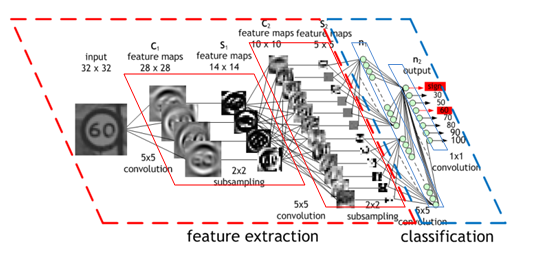
\includegraphics[scale=0.7]{convolutional_neural_network_structure} \]
  \centering
  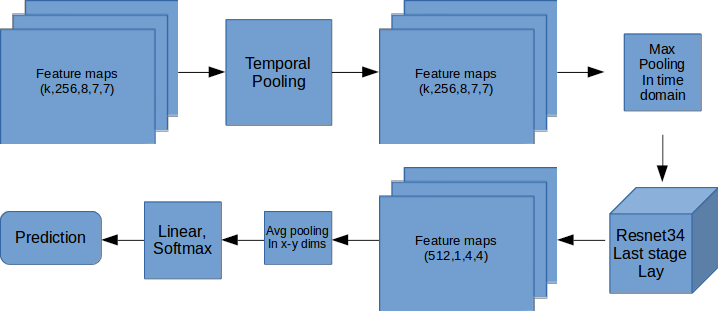
\includegraphics[scale=0.42]{mlp}
  \caption{Structure of the MLP classifier}
  \label{fig:mlp_structure}
\end{figure}
\gr
Σε προηγούμενες ενότητες χρησιμοποιήσαμε κλασσικούς ταξινομητές όπως τον Γραμμικό, ένα \en RNN \gr και \en SVM\gr.
Τελευταίoi αλλά εξίσου σημαντικoi, μια άλλη ευρέως κατηγορία ταξινομητών είναι οι \en Multilayer Perceptron (MLP)\gr.
Σχεδιάζουμε ένα MLP όπως φαίνεται στο σχήμα \ref{fig:mlp_structure} για διάρκεια δείγματος ίση με 8, και περιγράφεται κατωτέρω:

\begin{itemize}
\item Στην αρχή, μετά το \en 3D Roi Align \gr και για  διάρκεια του δείγματος ίση με  8 καρέ,
λαμβαουμε ένα χάρτη ενεργοποίησης μεγέθους  $(k, 256, 8, 7, 7)$ όπου k είναι ο αριθμός των συνδεδεμένων ToIs. Εμπνευσμένοι
από προηγούμενες ενότητες, εκτελούμε \en temporal pooling \gr ακολουθούμενο  από
\en max pooling \gr  στην  διάσταση της διάρκειας του δείγpματος. Έτσι, έχουμε τώρα έναν χάρτη χαρακτηριστικών 
με διαστάσεις ίσες με (2, 256, 7, 7), τις οποίες αναδιαμορφώνουμε σε
(256, 2, 7, 7) και τροφοδοτούμε \en layers \gr που εξήχθησαν από το τελευταίο στάδιο του \en ResNet34\gr.
Αυτά τα στάδια περιλαμβάνουν 3 \en Residual Layers \gr  με stride  ίσο με 2 σε όλες τις 3
διαστάσεις και αριθμός εξόδου φίλτρων ίσου με 512.
\item Μετά τα \en Residual Layers\gr, κάνουμε \en avg pooling \gr για τις διαστάσεις x-y.
Έτσι, έχουμε ως χάρτες ενεργοποίησης εξόδου με μέγεθος διαστάσεων ίσο με (512,).
Τέλος, τροφοδοτούμε  αυτoύς  τους  χαρακτηριστικούς  χάρτες σε ένα γραμμικό \en layer \gr προκειμένου να εξάγουμε την κλάση
του υποψήφιου \en action tube, \gr μετά την εφαρμογή της λειτουργίας Soft-Max.
\end{itemize}

\subsection{Κλασσικό \en training}
Όπως προαναφέρθηκε προηγουμένως, ο κώδικας εκπαίδευσης απαιτεί την εκτέλεση ενός μόνο βίντεο ανά GPU, επειδή τα βίντεο έχουν διαφορετική διάρκεια.
Για προηγούμενες προσεγγίσεις, μας ήρθδε η  ιδέα του προυπολογισμού των χαρακτηριστικά των \en action tubes \gr του βίντεο και στη συνέχεια
εκπαιδεύουμε μόνο τον ταξινομητή. Ωστόσο, για αυτό το βήμα, εκπαιδεύσαμε τον ταξινομητή μας με τον κλασιικό τρόπο για να λάβουμε
αποτελέσματα ταξινόμησης. Φυσικά, χρησιμοποιήσαμε ένα προεκπαιδευμένο \en TPN\gr, του οποίο παγώσαμε τα \en layers \gr για να μην εκπαιδευτούν.
Προσπαθήσαμε να εξερευνήσουμε διαφορετικές αναλογίες μεταξύ του αριθμού των \en action tubes \gr προσκηνίου και του συνολικού αριθμού των
\en action tubes \gr ανά βίντεο. Οι πρώτες 3 προσομοιώσεις περιλαμβάνουν σταθερό αριθμό συνολικών \en action tubes \gr και μεταβλητή αναλογία
μεταξύ του αριθμού των \en action tubes \gr προσκηνίου και φόντου. Αρχίσαμε χρησιμποιώντας μόνο \en action tubes \gr προσκηνίου, το  οποίο
σημαίνει ότι 32 από 32 \en action tube  \gr είναι προσκηνίου, μετά τα μισά από τα προτεινόμενα  \en action tubes, \gr δηλαδή 16 από 32 και
τέλος λιγότερο από το ήμισυ, δηλαδή 14 από τις 32.
Μετά από αυτό, πειραματιζόμαστε χρησιμοποιώντας έναν σταθερό αριθμό \en action tubes \gr προσκηνίου και μεταβλητού αριθμού συνολικών, o oποίος είναι 16, 24 και 32. Τα αποτελέσματα των επιδόσεων παρουσιάζονται στον πίνακα \ref{table:mlp_reg}.

\begin{center}
  \en
  \begin{longtable}{|| c | c || c c c ||}
    \hline
    \multirow{2}{*}{\textbf{FG tubes}} & \multirow{2}{*}{\textbf{Total tubes}} & {} &  \textbf{mAP} & {} \\
    {} & {} & 0.5 & 0.4 & 0.3 \\
    \hline
    32 & \multirow{3}{*}{32} &1.28 & 1.73 & 1.87  \\
    \cline{1-1} \cline{3-5}
    16 & {} & 3.98 & 4.38 & 4.38  \\
    \cline{1-1} \cline{3-5}
    14 & {} & 0.40 & 0.40 & 0.40 \\
    \hline
    \multirow{3}{*}{8} & 16 & 9.41 & 12.59 & 14.61 \\
    \cline{2-5}
    {} & 24 & 12.32 & 15.53 & 18.57 \\
    \cline{2-5}
    {} & 32 & 7.16 & 10.92 & 13.00 \\
    \hline
    \caption{MLP's mAP performance for regular training procedure}
    \label{table:mlp_reg}
  \end{longtable}
\end{center}

Τα αποτελέσματα δείχνουν ότι όταν οι πρώτες 3 προσεγγίσεις μας δίνουν πολύ άσχημα αποτελέσματα.
Συγκρίνοντας τους με τους υπόλοιπους 3, ήρθαμε με το συμπέρασμα ότι χρειαζόμαστε
το πολύ 8 \en action tubes \gr προσκηνίου, ακόμη και όταν ο λόγος μεταξύ του αριθμού \en action tubes \gr
του προσκηνίου και του φόντου είναι υπέρ του δεύτερου. Πιθανότατα, πάρα πολλοί
\en action tubes \gr προσκηνίου κάνουν την αρχιτεκτονική μας να έρθει σε κατάσταση \en overfitting \gr και
συνεπώς να είναι ανίκανη να γενικεύει.

\subsection{Εξαγωγή χαρακτηριστικών}

Όπως εκτελέστηκε προηγουμένως, εκπαιδεύσαμε τον ταξινομητή \en MLP \gr χρησιμοποιώντας προ-υπολογισμένους
χάρτες χαρακτηριστικών. Αυτοί οι χάρτες περιλαμβάνουν τόσο \en action tubes \gr που είναι στο  προσκήνιο όσο φόντου. Με
βάση τα συμπεράσματα που προέκυψαν  στα προηγούμενα τμήματα, θα εκπαιδεύσουμε
μόνο για  αριθμό \en action tube \gr προσκηνίου ίσο με 4 και 8. Επιπλέον
Θα  εκπαιδεύσουμε τον ταξινομητή μας για 3 διαφορετικές αναλογίες, οι οποίες είναι 1:1, 1:2 και 1:3.
Ο πίνακας \ref{table:mlp_extract_jhdmb} δείχνει αυτές τις περιπτώσεςι καθώς 
και τις αντίστοιχες επιδόσεις του \en mAP \gr κατά τη διάρκεια του βήματος επικύρωσης.
\begin{center}
  \en
  \begin{longtable}{|| c | c || c c c ||}
    \hline
    \multirow{2}{*}{\textbf{FG tubes}} & \multirow{2}{*}{\textbf{Total tubes}} & {} & \textbf{mAP} & {} \\
    {} & {} & 0.5 & 0.4 & 0.3 \\
    \hline
    \multirow{3}{*}{4} & 6 & 4,37 & 8,54 & 10,12 \\
    \cline{2-5}
    {} & 8 & 5.89 & 9.54 & 13.61 \\
    \cline{2-5}
    {} & 12 & 9.51 & 12.8 & 14.6  \\
    \cline{2-5}
    {} & 16 & 6.80 & 13.17 & 14.67 \\
    \hline
    \multirow{4}{*}{8} & 12 & 8,62 & 12,32 & 14,74 \\
    \cline{2-5}
    {} & 16 & 8.49 & 13.94 & 15.09 \\
    \cline{2-5}
    {} & 24 & 6.72 & 12.17 & 15.30 \\
    \cline{2-5}
    {} & 32 & 13.27 & 17.64 & 18.97 \\
    \hline

  \caption{mAP results for MLP trained using extracted features}
  \label{table:mlp_extract_jhdmb}
\end{longtable}
\end{center}

Συγκρίνοντας τα αποτελέσματα από τους πίνακες \ref{table:mlp_extract_jhdmb}  και \ref{table:mlp_reg}, είναι σαφές ότι χρειαζόμαστε 8
\en tubes \gr προσκηνίου για να λειτουργεί καλά ο ταξινομητής \en MLP. \gr  Ωστόσο, δεν είναι πολύ σαφές ποια από
τις  δύο προτεινόμενες εκπαιδευτικές διαδικασίες είναι καλύτερη, αλλά αν πρέπει να αποφασίσουμε μία
μέθοδο, θα επιλέξουμε τη χρήση προϋπολογισμένων χαρακτηριστικών. Η προσέγγιση αυτή
κατορθώνει να επιτύχει τα καλύτερα αποτελέσματα, και ειδικά όταν έχουμε 8
\en tubes \gr προσκηνίου και 32 συνολικά. Επίσης, συγκρίνοντας τις μεθόδους με 4 ή 8 θετικά
\en action tubes\gr, είναι σαφές ότι θα προτιμούσαμε να χρησιμοποιούμε 8 γενικά. Ωστόσο, δεν είναι
σαφές ποια αναλογία είναι καλύτερη, επειδή, έχουμε καλύτερα αποτελέσματα όταν έχουμε 8
\en action tubes \gr και αναλογία 1:4 ενώ έχουμε καλύτερα αποτελέσματα όταν η αναλογία είναι 1:3
με 4 \en action tubes.\gr

\section{\en UCF dataset\gr}
\subsection{Εισαγωγή}
Κατά τη διάρκεια της προηγούμενης ενότητας, διερευνούμε διαφορετικές μεθόδους ταξινόμησης χρησιμοποιώντας
διάφορες τάξεις.  Λαμβάνοντας υπόψη την απόδοση των \en recall \gr και \en MABO \gr που παρουσιάζονται στο κεφάλαιο 4,
είναι σαφές ότι το δίκτυό μας θα αποτύχει να αναγνωρίσει τα περισσότερα πραγματικά
 χωροχρονικά \en action tubes \gr και να τα ταξινομήσει σωστά. Ωστόσο
στις περισσότερες περιπτώσεις, η απόδοση του MABO πήρε Βαθμολογία περίπου 92-94\%. Οπότε, μας ήρθε η ιδέα
 να μην εκτελέσουμε  χωροχρονικό εντοπισμό και ταξινόμηση,
για το σύνολο δεδομένων \en UCF\gr, αλλά μόνο χρονικό εντοπισμό. Αυτό σημαίνει ότι
προσπαθούμε να ανιχνεύσουμε  τα τμήματα βίντεο στα οποία εκτελείται μια ενέργεια, και επίσης προσπαθούμε
 να προσδιορίσουμε την κλάση της εκτελεσμένης ενέργειας.
\subsection{Χρονικός εντοπισμός}

Όπως παρουσιάζεται στο κεφάλαιο 4, ο αλγόριθμος σύνδεσής μας είναι σε θέση να πάρει καλή απόδοση χρονικού 
\en recall \gr και  \en MABO\gr. Για τον χρονικό εντοπισμό μιας  δράσης σε
βίντεο, χρησιμοποιούμε μόνο τις χρονικές πληροφορίες που περιέχουν  τα προτεινόμενα \en action tubes\gr,
που ισοδυναμούν με το πρώτο και το τελευταίο καρέ του \en tube\gr. Θα ταξινομήσουμε τα προτεινόμενα \en action tubes \gr
χωρίς να πραγματοποιήσουμε χωροχρονικό εντοπισμό, αλλά μόνο χρονικό. Αν και δεν χρησιμοποιούμε τα προτεινόμενα πλαίσια ανά καρέ
για την ταξινόμηση, εκμεταλλευόμταστε τις χωρικές πληροφορίες τους για να
να εκτελέσουμε  καλύτερo χρονικό εντοπισμό. Διαισθητικά, αυτό συμβαίνει επειδή, για να
να εξαγάγουμε τα \en action tubes\gr, λαμβάνουμε υπόψιν μας τη χωρική επικάλυψη μεταξύ των συνδεδεμένων \en ToIs\gr.

Η προαναφερθείσα προσέγγιση περιλαμβάνει τα ακόλουθα βήματα:
\begin{enumerate}
\item Αρχικά, χρησιμοποιούμε το \en TPN  \gr για να προτείνουμε χωροχρονικά ToIs, όπως ακριβώς κάναμε
στις προηγούμενες προσεγγίσεις. Στη συνέχεια, συνδέουμε αυτά τα ToIs με βάση τον προτεινόμεν αλγόριθμο
του κεφαλαίου 4, με τη χρήση του χωροχρονικoύ αλγορίθμου \en NMS \gr με κατώφλι σύνδεσης
 ίσο με 0,9, για την αφαίρεση επικαλυπτόμενων \en action tubes\gr.
\item Tα επόμενα βήματα είναι ακριβώς τα ίδια με τις προηγούμενες προσεγγίσεις ταξινόμησης.
Ωστόσο, σε αυτή την προσέγγιση, δεν χρησιμοποιούμε κανένα είδος \en ROI Aling \gr για να
εξάγουμε τους χάρτες χαρακτηριστικών των \en action tubes\gr. Αντιθέτως, για όλες τις προτεινόμενες
ακολουθίες από πλαίσια, βρίσκουμε τη διάρκειά τους, δηλαδή  το πρώτο και τελευταίο τους καρέ.
Μετά από αυτό, τρέχουμε τον αλγόριθμο του χρονικόυ \en NMS \gr  για να αφαιρέσουμε  αλληλοεπικαλυπτόμενα \en action tubes\gr.
 Η μόνη διαφορά μεταξύ του χωροχρονικού και χρονικόυ \en NMS \gr είναι ο
το κριτήριο επικάλυψης, το οποίο χρησιμοποιείται. Για τα χωροχρονικό \en NMS \gr χρησιμοποιούμε το τρισδιάστατο \en IoU, \gr ενώ 
 αντίστοιχα, για το χρονικό \en NMS, \gr το μονοδιάστατο.

\item Φυσικά, τα προτεινόμενα \en action tubes \gr διαρκούν περισσότερο από 16 καρέ
  που ορίζεται ως διάρκεια δείγματος. Έτσι, διαχωρίζουμε τα προτεινόμενα \en action tubes \gr σε βίντεο κλιπ
  διάρκειας 16 καρέ (όπως η διάρκεια του δείγματός μας). Αυτά τα τμήματα βίντεο δίνονται ως είσοδο
και πάλι σε ένα  3D resNet34 (\cite{hara3dcnns}), το οποίο, αυτή τη φορά, δεν το χρησιμοποιούμε μόνο για
 εξαγωγής χαρακτηριστικών, αλλά και για ταξινόμηση  κάθε τμήματος βίντεο.
\item Έτσι, για κάθε βίντεο κλιπ, για κάθε κλάση έχουμε ένα σκορ εμπιστοσύνης μετά την
λειτουργία του softmax. Τέλος, υπολογίζουμε τη μέση βαθμολογία εμπιστοσύνης για
σε κάθε κλάση, και θεωρούμε την κλάση με τη βέλτιστη βαθμολόγηση ως ετικέτα του 
\en action tube\gr. Φυσικά, μερικα \en action tubes \gr μπορεί να μην περιέχουν καμία ενέργεια,
Έτσι έχουμε ορίσει ένα κατώφλι  εμπιστοσύνης για ξεχωρίσουμε τα \en action tubes  \gr  προσκηνίου με αυτά του
φόντο.
\end{enumerate}
\paragraph{\tl{Training}} Το μόνο εκπαιδεύον μέρος αυτής της αρχιτεκτονικής είναι το ResNet34. Χρησιμοποιούμε
ένα προεκπαιδευμένο TPN, όπως παρουσιάζεται στο κεφάλαιο 4. Η διαδικασία κατάρτισης ResNet34
με βάση τον κωδικό που δόθηκε από το [?]. Το τροποποιήσαμε για να μπορούμε να εκπαιδευόμαστε
για το σύνολο δεδομένων UCF-101, μόνο για τις 24 τάξεις, για τις οποίες υπάρχουν
και η TPN μας είναι εκπαιδευμένη.
\paragraph{\tl{Validation}} Με βάση τα προαναφερθέντα βήματα, είναι σαφές ότι οι παράμετροι
που μπορούν να τροποποιηθούν είναι τα χρονικά όρια και το όριο
να αποφασίζουν εάν μια ενέργεια περιέχεται ή όχι. Όλοι οι διαφορετικοί συνδυασμοί που χρησιμοποιούνται
κατά τη διάρκεια της επικύρωσης παρουσιάζονται στον πίνακα 1,20.

\begin{center}
  % \setlength{\tabcolsep}{2pt}
  \begin{longtable}{|| c | c || c c c ||}

    \hline
    \multirow{2}{*}{\textbf{NMS thresh}} & \multirow{2}{*}{\textbf{Conf thresh}} & {} & \textbf{mAP} & {}  \\
    {} & {} & 0.5 & 0.4 & 0.3\\
    \hline
    \multirow{3}{*}{0.9} & {0.6} & 0.3 & 0.54 & 0.64 \\
    \cline{2-5}
    {} & {0.75} & 0.25 & 0.45 & 0.55 \\
    \cline{2-5}
    {} & {0.85} & 0.2 & 0.38 & 0.49  \\
    \hline
    \multirow{3}{*}{0.7} & {0.6} & 0.63 & 1.02 & 1.27 \\
    \cline{2-5}
    {} & {0.75} & 0.5 & 0.84 & 1.05 \\
    \cline{2-5}
    {} & {0.85} & 0.4 & 0.68 & 0.89 \\
    \hline
    \multirow{3}{*}{0.5} & {0.6} & 0.96 & 1.21 & 1.75 \\
    \cline{2-5}
    {} & {0.75} &  0.63 & 0.93 & 1.38 \\
    \cline{2-5}
    {} & {0.85} & 0.57 & 0.72 & 1.03 \\
    \hline
    \multirow{3}{*}{0.4} & {0.6} & 1.07 & 1.52 & 2.03 \\
    \cline{2-5}
    {} & {0.75} &  0.79 & 1.18 & 1.63 \\
    \cline{2-5}
    {} & {0.85} & 0.71 & 0.98 & 1.33 \\
    \hline
    \multirow{3}{*}{0.3} & {0.6} & 1.1 & 1.66 & 2.53 \\
    \cline{2-5}
    {} & {0.75} &  0.93 & 1.39 & 2.08 \\
    \cline{2-5}
    {} & {0.85} & 0.81 & 1.12 & 1.6 \\
    \hline
    \multirow{3}{*}{0.2} & {0.6} & 0.84 & 1.38 & 2.17 \\
    \cline{2-5}
    {} & {0.75} & 0.73 & 1.13 & 1.78 \\
    \cline{2-5}
    {} & {0.85} & 0.65 & 0.81 & 1.31 \\

    \hline

    \caption{UCF's temporal localization mAP performance}
    \label{table:temp_cls_1}
  \end{longtable}
\end{center}

\begin{center}
  % \setlength{\tabcolsep}{2pt}
  \begin{longtable}{|| c || c c c | c |}
    \hline
    \multirow{2}{*}{\textbf{NMS thresh}} & {} & {\textbf{Recall}} & {} & \multirow{2}{*}{\textbf{MABO}} \\
      {} & 0.9 & 0.8 & 0.7 & {} \\
      \hline
      0.9 & 0.7361 & 0.8935 & 0.9422 & 0.9138130172 \\
      \hline
      0.7 & 0.3194 & 0.6875 & 0.9293 & 0.8412186326 \\
      \hline
      0.5 & 0.1757 & 0.3331 & 0.6281 & 0.7471525429 \\
      \hline
      0.4 &0.1483 & 0.2829 & 0.4707 & 0.6986400756 \\
      \hline
      0.3 & 0.111 & 0.2038 & 0.3848 & 0.6429232202 \\
      \hline
    \caption{UCF's temporal localization recall and MABO performances}
    \label{table:temp_cls_recall_1}
  \end{longtable}
\end{center}

Σύμφωνα με τον πίνακα 1,20, οι επιδόσεις του mAP για τη χρονική
η ταξινόμηση είναι πολύ κακή. Η καλύτερη απόδοση είναι περίπου 2%,
πολύ χαμηλά. Συγκρίνοντας αυτά τα αποτελέσματα με τα αποτελέσματα που εμφανίζονται στον πίνακα 1,21, συμπεραίνουμε
ότι η μέθοδός μας δεν είναι καθόλου αποδοτική. Παρόλο που τα αποτελέσματα του mAP αυξάνονται
και η απόδοση του MABO μειώνεται ταχέως. Φυσικά, αυτό το αποτέλεσμα
Δεδομένου ότι, μειώνοντας το όριο του νμμs, ο αριθμός των απορριπτθέντων
σωλήνες δράσης αυξάνεται.
Δοκιμάσαμε μια άλλη προσέγγιση, η οποία εφαρμόζει τον αλγόριθμο
και όχι πριν από αυτό όπως κάναμε προηγουμένως. Επίσης, παρατηρήσαμε σε προηγούμενες
στις περισσότερες περιπτώσεις, έχουμε αυτές τις χαμηλές επιδόσεις λόγω της
με ψευδή θετικά αποτελέσματα, τα οποία δεν αφαιρούνται κατά τη διάρκεια της διαδικασίας. Να είμαι
πιο συγκεκριμένα, ο πίνακας 1,22 δείχνει όλα τα πραγματικά και ψευδώς θετικά
ορίζεται το όριο του ννs ίσο με 0,2, όριο επικάλυψης mAP ίσο με 0,3
και όριο εμπιστοσύνης ίσο με 0,6 για τις δύο προαναφερθείσες προσεγγίσεις.

\begin{center}
  \setlength{\tabcolsep}{2pt}
  \begin{longtable} {|| c | c c | c c | c | cc | cc||}

    \hline
    \multirow{2}{*}{\textbf{Class}} & \multicolumn{2}{|c|}{\textbf{Appr 1}}  & \multicolumn{2}{ c||}{\textbf{Appr 2}} &
    \multirow{2}{*}{\textbf{Class}} & \multicolumn{2}{|c|}{\textbf{Appr 1}}  & \multicolumn{2}{ c||}{\textbf{Appr 2}} \\
    {} & TP & FP & TP & FP &
    {} & TP & FP & TP & FP \\
    \hline    
    Basketball & 5 & 279 & 6 & 403 &
    BasketballDunk & 7 & 7 & 12 & 13 \\
    Biking & 0 & 3 & 0 & 5 &
    CliffDiving & 11 & 55 & 1 & 1 \\
    CricketBowling &  0 & 0 & 10 & 75 &
    Diving & 20 & 189 & 23 & 272 \\
    Fencing & 11 & 222 & 25 & 336 &
    FloorGymnastics & 2 & 86 & 6 & 131 \\
    GolfSwing & 4 & 51 & 6 & 78&
    HorseRiding & 0 & 33 & 4 & 58 \\
    IceDancing & 8 & 29 & 6 & 38 &
    LongJump & 1 & 24 & 6 & 43 \\
    PoleVault & 0 & 202 & 9 & 296 &
    RopeClimbing & 1 &24 & 4 & 43 \\
    SalsaSpin & 3 & 158 & 5 & 237 &
    SkateBoarding & 0 & 10 & 0 & 13 \\
    Skiing & 0 & 0 & 0 & 0 &
    Skijet & 1 & 27 & 6 & 43 \\
    SoccerJuggling & 3 & 94 & 1 & 153 &
    Surfing  & 11 & 102 & 23 & 159 \\
    TennisSwing & 0 & 125 & 0 & 166 &
    TrampolineJumping & 4 & 18 & 4 & 32 \\
    VolleyballSpiking & 20 &704 & 20 & 1044 &
    WalkingWithDog & 0 & 5 & 0 & 9 \\
    \hline    
    \caption{Comparing TP and FP for both approaches}
    \label{table:tp_fp}

  \end{longtable}
\end{center}

Λαμβάνοντας υπόψη αυτά τα δύο γεγονότα, ήρθαμε με την ακόλουθη λύση. Στην
προσέγγιση, ταξινομήσαμε τους υποψήφιους σωλήνες δράσης χρησιμοποιώντας βαθμολογίες σύνδεσης που
από τη σύνδεση του αλγορίθμου και μετά αφαιρέσαμε τους σωλήνες δράσης. In
η νέα προσέγγισή μας, αφαιρούμε πρώτα τους σωλήνες δράσης με τα ίδια χρονικά όρια,
για να πάρετε μοναδικούς σωλήνες χρονικής δράσης. Στη συνέχεια, ταξινομούμε όλες τις προτεινόμενες
σωλήνες δράσης ακριβώς όπως κάναμε στο βήμα 3 προηγουμένως. Μετά από αυτό, θα εκτελέσουμε
με τις βαθμολογίες εμπιστοσύνης που εξάγονται από το τελευταίο στρώμα της
3D ResNet34 και τέλος κρατάμε αυτά που το σκορ εμπιστοσύνης τους είναι πάνω από ένα
προκαθορισμένο όριο.
\begin{center}
  % \setlength{\tabcolsep}{2pt}
  \begin{longtable}{|| c | c || c c c ||}

    \hline
    \multirow{2}{*}{\textbf{NMS thresh}} & \multirow{2}{*}{\textbf{Conf thresh}} & {} & \textbf{mAP} & {}  \\
    {} & {} & 0.5 & 0.4 & 0.3\\
    \hline
    \multirow{3}{*}{0.9} & {0.6} & 0.31 & 0.54 & 0.65 \\
    \cline{2-5}
    {} & {0.75} & 0.26 & 0.46 & 0.55 \\
    \cline{2-5}
    {} & {0.85} & 0.2 & 0.39 & 0.49 \\
    \hline
    \multirow{3}{*}{0.7} & {0.6} & 0.66 & 0.95 & 1.22 \\
    \cline{2-5}
    {} & {0.75} & 0.55 & 0.80 & 1.01 \\
    \cline{2-5}
    {} & {0.85} & 0.41 & 0.67 & 0.87 \\
    \hline
    \multirow{3}{*}{0.5} & {0.6} & 0.98 & 1.43 & 1.63 \\
    \cline{2-5}
    {} & {0.75} & 0.75 & 1.14 & 1.29 \\
    \cline{2-5}
    {} & {0.85} & 0.64 & 0.92 & 1.04 \\
    \hline
    \multirow{3}{*}{0.4} & {0.6} & 1.19 & 1.73 & 2.15 \\
    \cline{2-5}
    {} & {0.75} & 0.9 & 1.35 & 1.63 \\
    \cline{2-5}
    {} & {0.85} & 0.79 & 1.16 & 1.38 \\

    \hline
    \multirow{3}{*}{0.3} & {0.6} & 1.12 & 1.85 & 2.23 \\
    \cline{2-5}
    {} & {0.75} & 0.96 & 1.54 &1.7 \\
    \cline{2-5}
    {} & {0.85} & 0.83 & 1.28 & 1.43 \\
    \hline
    \multirow{3}{*}{0.2} & {0.6} & 2.05 & 2.68 & 3.7 \\
    \cline{2-5}
    {} & {0.75} & 1.61 & 2.17 & 3 \\
    \cline{2-5}
    {} & {0.85} & 1.51 & 1.88 & 2.54 \\

    \hline

    \caption{UCF's temporal localization mAP performance}
    \label{table:temp_cls_2}
  \end{longtable}
\end{center}

Συγκρίνοντας τους πίνακες 1,23 και 1,21, έχουμε τα ίδια αποτελέσματα για την επικάλυψη
κατώτατα όρια 0,9, 0,7, 0,5, 0,4 και 0,3. Αλλά για επικάλυψη όριο 0,2 έχουμε παρατηρήσει
Οι επιδόσεις του mAP βελτιώνονται περίπου στο 1%. Έτσι, σκεφτήκαμε ότι θα πρέπει να
να χρησιμοποιούν ακόμη μικρότερα κατώτατα όρια επικάλυψης, τα οποία είναι 0,15, 0,1 και 0,05 τα οποία
παρουσιάζονται στον πίνακα 1,24.

\begin{center}
  \begin{longtable}{|| c | c | c c c||}
    \hline
    \multirow{2}{*}{\textbf{NMS thresh}} & \multirow{2}{*}{\textbf{Conf thresh}} & {} & \textbf{mAP} & {} \\
    {} & {} & 0.5 & 0.4 & 0.3 \\
    \hline
    \multirow{3}{*}{0.15} & 0.6 & 2.01 & 2.66 & 3.62 \\
    \cline{2-5}
    {} & 0.75 & 1.62 & 2.21 & 2.97 \\
    \cline{2-5}
    {} & 0.85 & 1.51 & 1.91 & 2.56 \\
    \hline
    \multirow{3}{*}{0.10} & 0.6 & 1.87 & 2.74 & 3.77 \\
    \cline{2-5}
    {} & 0.75 & 1.62 & 2.28 & 3.08  \\
    \cline{2-5}
    {} & 0.85 & 1.5 & 2 & 2.7  \\
    \hline
    \multirow{3}{*}{0.05} & 0.6 & 1.85 & 2.71 & 3.73  \\
    \cline{2-5}
    {} & 0.75 & 1.61 & 2.28 & 3.1  \\
    \cline{2-5}
    {} & 0.85 & 1.5 & 2 & 2.7 \\
    \hline

    \caption{UCF's temporal localization mAP performance for even smaller NMS threshold}
    \label{table:temp_cls_2_1}

  \end{longtable}
\end{center}

Η χρήση πολύ μικρού κατώτατου ορίου του ΝS οδηγεί σε μια μικρή βελτίωση του mAP
Απόδοση. Ωστόσο, αυτές οι βαθμολογίες απέχουν πολύ από τα υπερκαλλιτεχνικά αποτελέσματα.
Έτσι, νομίζουμε ότι πρέπει να επανεξετάσουμε τον τρόπο που εκπαιδεύσαμε την τάξη μας και την
τον τρόπο με τον οποίο ταξινομεί τους σωλήνες δράσης, προκειμένου να είναι σε θέση να ταξινομήσει αποτελεσματικά.
Αυτή η έρευνα έχει απομείνει για μελλοντικές εργασίες, και δεν θα γίνει ανάληψη καθηκόντων σε αυτή τη διατριβή.

\end{document}
% \documentclass{report}

% \usepackage[ english, greek]{babel}
% \usepackage[utf8]{inputenc}
% \usepackage[LGR, T1]{fontenc}

% % % 

% \newcommand{\tl}{\textlatin}
% \newcommand{\en}{\selectlanguage{english}}
% \newcommand{\gr}{\selectlanguage{greek}}

% \usepackage{hyperref}  % package for linking figures etc
% \usepackage{enumitem}  % package for description with bullets
% \usepackage{graphicx}  % package for importing images
% \usepackage{mathtools} % package for math equation
% \usepackage{mathrsfs}  % package for math font
% \usepackage{indentfirst} % package for getting ident after section or paragraph
% \usepackage{subcaption} % package for subfigures
% \usepackage[export]{adjustbox}
% \usepackage{longtable} % package for multi pages tables
% \usepackage{multirow}  % package for tables, multirow
% \usepackage{amssymb}
% \usepackage{esvect}
% \usepackage[
% backend=bibtex,
% citestyle=authoryear,
% % citestyle=authoryear-comp,
% % citestyle=authoryear-ibid,
% bibstyle=numeric,
% sorting=ynt,
% % style=numeric,
% % style=alphabetic ,
% ]{biblatex}
% \addbibresource{References}

% \graphicspath{ {./theory/figures/} }       % path for images

% \begin{document}
\gr 

\chapter{Επίλογος - Μελλοντικές επεκτάσεις}
\section{Επίλογος}
Σε αυτή τη διατριβή εξερευνήσαμε το πρόβλημα της αναγνώρισης και του εντοπισμού ανθρώπινης δράσης σε βίντεο.
Σχεδιάσαμε  ένα δίκτυο βασισμένο στην προσέγγιση των  \cite{DBLP:journals/corr/HouCS17} σε συνδυασμό με ορισμένα στοιχεία από τους \en\cite{DBLP:journals/corr/abs-1712-09184},
\cite{Ren:2015:FRT:2969239.2969250}, \cite{Girshick:2015:FR:2919332.2920125}, \cite{DBLP:journals/corr/abs-1903-00304} \gr
 και \en \cite{hara3dcnns}\gr. \par

 Γράψαμε μια \en pytorch \gr υλοποίηση παίρνοντας κώδικα  μόνο από το \en \cite{jjfaster2rcnn}\gr. Επιπλέον, γράψαμε τον δικό μας κώδικα χρησιμοποιώντας
 μερικές λειτουργίες της γλώσσας \en CUDA \gr που έχουν σχεδιαστεί από εμάς (όπως
υπολογισμός των βαθμολογιών σύνδεσης, τροποποίηση \tl{tubes} κλπ). \par

Προσπαθήσαμε να σχεδιάσουμε   το \en TPN\gr, ένα δίκτυο  που εξάγει \en ToIs, \gr ακολουθίες πλαισίων  δηλαδή, που πιθανώς να περιέχουν κάποια δράση  
σε δεδομένο τμήμα του βίντεο, εμπνευσμένο από το \en  RPN \gr  του \en Faster R-CNN\gr. To σχεδιάσαμε
χρησιμοποιώντας γενικευμένα \en anchors \gr  και όχι συγκεκριμένα για κάθε σύνολο δεδομένων. Προσπαθούμε δηλαδή
να γενικεύσουμε την προσέγγισή μας για διάφορα σύνολα δεδομένων, αντίθετα με την προσέγγιση
που προτείνεται από τους \en \cite{DBLP:journals/corr/abs-1712-09184}\gr, στην οποία χρησιμοποιoύνται τα πιο συχνά εμφανιζόμενα
\en anchors \gr για κάθε σύνολο δεδομένων.

Επιπροσθέτως, σχεδιάσαμε έναν αφελή αλγόριθμο σύνδεσης για τη σύνδεση
των προτεινόμενων \en ToIs \gr  με βάση αυτόν που προτάθηκε απ' τους \en \cite{DBLP:journals/corr/abs-1712-09184}\gr.
Στην προσέγγισή μας, χρησιμοποιούμε την ίδια πολιτική βαθμολόγησης, η οποία είναι ένας συνδυασμός των βαθμολογιών της πιθανότητας ύπαρξης δράσης και του σκορ επικάλυψης.
Η κύρια διαφορά είναι ότι αποφεύγουμε να υπολογίζουμε
πιθανούς συνδυασμούς, χρησιμοποιώντας ένα όριο ενημέρωσης, που μπορεί να ανανεώνεται. Επίσης, δοκιμάσαμε κι άλλον έναν
αλγόριθμο σύνδεσης εμπνευσμένος απ' τους \cite{DBLP:journals/corr/abs-1903-00304}.
Ωστόσο, η εφαρμογή μας δεν ήταν τόσο καλή όσο η προηγούμε, συνεπώς δεν εξερευνήσαμε όλες τις δυνατότητες του.

Τέλος, διερευνήσαμε αρκετούς ταξινομητές  για το στάδιο ταξινόμησης του
δικτύου. Αυτοί είναι: έναν \en RNN\gr, ένα Γραμμικό ταξινομητή, έναν \en SVM \gr  και έναν ταξινομητή \en MLP\gr.
Χρησιμοποιήσαμε μια εφαρμογή απ' το  Fast RCNN για τον ταξινομητή  \en SVM\gr, η οποία περιελάμβανε την διαδικασία
εκπαίδευσης μέσω σκληρών αρνητικών. Εξετάσαμε μερικές τεχνικές εκπαίδευσης για
βέλτιστη απόδοση ταξινόμησης και 2 εκπαιδευτικές προσεγγίσεις για τον ταξινομητή \en MLP\gr, την κλασσική και μία που
χρησιμοποιούμε προεξαγόμενα χαρακτηριστικά.

\section{Μελλοντικές επεκτάσεις}

Υπάρχουν πολλά περιθώρια βελτίωσης για το δίκτυό μας, προκειμένου να επιτευχθεί
τελευταίας τεχνολογίας αποτελέσματα. Οι σημαντικότερες περιγράφονται στις επόμενες παραγράφους.

\paragraph{Βελτίωση των προτάσεων του \en TPN\gr}

Υλοποιήσαμε 2 δίκτυα για την πρόταση ακολουθιών από πλαίσια σε ένα τμήμα βίντεο. Πετύχαμε περίπου 63\% βαθμολογία \en recall \gr
για τη διάρκεια του δείγματος ίση με 16 καρέ και περίπου 80\% \en recall \gr για τη διάρκεια του δείγματος ίση με 8. Αυτά τα σκορ 
δείχνουν ότι υπάρχει αρκετός χώρος για βελτίωση ειδικά για την περίπτωση με δείγμα 16 καρέ.
Παρόλο που έχουν διερευνηθεί πολλές αρχιτεκτονικές δικτύων για
παλινδρόμηση, μια καλή ιδέα θα ήταν να δοκιμάσουμε άλλα δίκτυα, τα οποία δεν είναι απαραίτητα εμπνευσμένη
από δίκτυα εντοπισμού αντικειμένων όπως κάναμε εμείς. 
Επιπλέον, προσθέτοντας έναν παράγοντα \textit{λ} στον τύπο του \en training loss \gr
 θα ήταν μια καλή ιδέα και θα διερευνούσε ποια είναι η καλύτερη προσέγγιση αυτού.
Έτσι, η απώλεια εκπαίδευσης θα μπορούσε να οριστεί ως:
\begin{equation} 
\begin{split}
 L  =  \sum_iL_{cls}(p_i, p_i^*) + \lambda_1 \sum_ip_i^*L_{reg}(t_i,t_i^*) + \lambda_2  \sum_iq_i^*L_{reg}(c_{i}, c_{i}^*) \\
\end{split}
\end{equation}
Επιπλέον, θα ήταν μια καλή ιδέα να χρησιμοποιήσουμε την μέθοδο του \en SSD  (\cite{DBLP:journals/corr/LiuAESR15}) \gr που προτείνει \en RoIs \gr 
αντί για το \en RPN\gr, για να συγκρίνουμε το αποτέλεσμα.  Τέλος, θα μπορούσαμε να πειραματιστούμε χρησιμοποιώντας τα δίκτυα \en Feature Pyramid (\cite{8099589}), \gr
τα οποία θα μπορούσαν να επεκταθούν σε 3 διαστάσεις ως ένα άλλο δίκτυο εξαγωγής χαρακτηριστικών ή κάποιο άλλο είδος \en 3D ResNet\gr.

\paragraph{Αλλαγή του αλγορίθμου σύνδεσης}
Σε αυτή τη διατριβή, μια άλλη πρόκληση που αντιμετωπίσαμε ήταν η σύνδεση των προτεινόμενων \en ToIs \gr για την πρόταση \en action tubes\gr. Υλοποιήσαμε έναν πολύ αφελή αλγόριθμο,
που δεν ήταν σε θέση να μπορεί να μας δώσει πολύ καλές προτάσεις παρά τις αλλαγές που προσπαθήσαμε να κάνουμε. Υλοποιήσαμε έναν άλλο αλγόριθμο σύνδεσης που ήταν βασισμένος στην εκτίμηση της χρονικής
πρόοδο ενός \en action tube \gr και την αλληλεπίδραση του με άλλα. Αν και δεν μας έδωσε και πολύ καλές προτάσεις, πιστεύουμε ότι πρέπει να εξερευνήσουμε τις δυνατότητες αυτού του αλγορίθμου. Κι αυτό 
επειδή είναι σε θέση να   εκμεταλλεύεται την πρόοδο της ενέργειας, την οποία δεν είχε ο προηγούμενος αλγόριθμος.

\paragraph{Εξερεύνηση άλλων τεχνικών ταξινόμησης}

Για το στάδιο ταξινόμησης, πειραματιστήκαμε κυρίως πάνω σε έναν ταξινομητή \en SVM  \gr για το σύνολο δεδομένων \en JHMDB \gr και δεν ασχοληθήκαμε καθόλου  με το σύνολο δεδομένων \en UCF-101\gr. Ο πρώτος μας
στόχος είναι να είμαστε σε θέση να εξάγουμε καλά αποτελέσματα ταξινόμησης για το σύνολο δεδομένων \en UCF-101\gr.  Πιστεύουμε ότι θα πρέπει να διερευνήσουμε τους χάρτες χαρακτηριστικών του \en UCF-101 \grκαι  τεχνικές  που εφαρμόζονται στους χάρτες χαρακτηριστικών πριν από την ταξινόμηση. Επιπλέον, θα μπορούσαμε να δοκιμάσουμε άλλες τεχνικές ταξινόμησης όπως \en Random Forests \gr ή να πειραματιστούμε περισσότερο με τον ταξινομητή \en RNN \gr για το σύνολο δεδομένων \en UCF-101\gr.
Τέλος, μια άλλη διαδικασία ταξινόμησης θα ήταν μια καλή ιδέα, όπως η εξαγωγή πρώτα όλων των πιθανών \en action tubes \gr και, στη συνέχεια, η χρήση άλλων δικτύων για εξαγωγή χαρακτηριστικών προκειμένου
να ταξινομήσουμε τα \en action tubes\gr.

\en
% \end{document}
\en
% \documentclass{report}

% \usepackage{subcaption} % package for subfigures
% \usepackage{hyperref}  % package for linking figures etc
% \usepackage{enumitem}  % package for description with bullets
% \usepackage{graphicx}  % package for importing images
% \usepackage{mathtools} % package for math equation
% \usepackage{mathrsfs}  % package for math font
% \usepackage{indentfirst} % package for getting ident after section or paragraph
% \usepackage[export]{adjustbox}
% % \usepackage{amsmath}

% \setlength{\parindent}{2em} % how much indent to use when we start a paragraph

% \graphicspath{ {./theory/figures/} }       % path for images

% \begin{document}

\chapter{Introduction}
Nowadays, the enormous increase of computing power help us deal with a lot of difficult situations appeared in our daily life.
A lot of areas of science have managed to tackle with problems, which were con-sided non trivial 20 years ago. One of
these area is Computer Vision and an important problem is human action recognition and localization.
\section{Problem statement}
The area of human action recognition and localization has 2 main goals:
\begin{enumerate}
\item Automatically detect and classify any human activity, which appears in a video.
\item Automatically locate in the video, where the previous action is performed.
\end{enumerate}

\subsection{Human Action Recognition}
Considering human action recognition, a video may be consisted of only by 1 person doing something. However, this is a ideal
situation. In most cases, videos contain multiple people, who perform multiple actions or may not act at all in some segments.
So, our goal is not only to classify an action, but to determine the temporal boundaries of each action.
\subsection{Human Action Localization}
Alongside with Human Action Recognition, another problem is to present spatial boundaries of each action. Usually, this means
presenting a 2D bounding box for each video frame, which contains the actor. Of course, this bounding box moves alongside with
the actor.

\section{Applications}
The field of Human Action Recognition and Localization has a lot of applications which include 
 content based video analysis,automated video segmentation, security and surveillance systems,
human-computer interaction.

The huge availability of data (especially of videos) create the  necessity to find ways to take advantage of them.
About 2.5 billion images are uploaded at Facebook database every month, more than 34K hours of video in YouTube and
about 5K images every minute. On top of that, there are about 30 million surveillance cameras in US, which means
about 700K video hours per day. All those data need to be separated in categories according to their content in
order to search them more easily. This process takes place by hand, by a user who attaches
keywords or tags to each video. However, most users avoid doing that, so many videos end up without any tagging information.
This situation creates the need to create algorithms for automated indexing based on the content of the video.

Another application is video summary. This area take place usually in movies or sports events. In movies,
video analysis algorithms can create a small video containing all the important moments of the movie. This
can be achieved by choosing video segments which an important action takes place such as killing the villain
of the movie. In sports events, video summary applications include creating highlight videos automatically, like
a video containing all achieved goals in football match.

On top of that, human action recognition can replace human operators in surveillance systems. Until now,
security systems include a system of multiple cameras handled by a human operator, who judges if a person
is acting normally or not. Automatic action classification systems can act like human, and immediately
judge if there is any human behavioral anomaly.

Last but not least, another field of application is related with human-computer interaction. Robotic applications
help elderly people deal with their daily needs. Also, gaming applications using Kinect create new kinds of
gaming experience without the need of a physical game controller.

\section{Challenges and Datasets}
There are various types of human activities. Depending on their complexity, we conceptually categorize human activities into four different
levels: gestures, actions, interactions, and group activities. Gestures are elementary movements of a person’s body part, and are the atomic
components describing the meaningful motion of a person. ``Stretching an arm'' and ``raising a leg'' are good examples of gestures.
Actions are single person activities that may be composed of multiple gestures organized temporally, such as ``walking'', ``waving'', and
``punching''. Interactions are human activities that involve two or more persons and/or objects. For example, ``two persons fighting'' is
an interaction between two humans and ``a person stealing a suitcase from another'' is a human-object interaction involving two humans and one
object. Finally, group activities are the activities performed by conceptual groups composed of multiple persons and/or objects. ``A group of persons marching'', ``a group having a meeting'', and ``two groups fighting'' are typical examples of them.
The wide variety of human activities and applications creates a lot of challenges which involve action recognition systems.
The most important challenges include large variations in appearance of the actors, camera view-point changes, occlusions,
non-rigid camera motions etc. On top of that, a big problem is that there are too many action classes which means
that manual collection of training sample is prohibitive. Also, some times, action vocabulary is not well defined.
As figure \ref{fig:open_example} shows, ``Open'' action can include a lot of kinds of actions, so we must carefully
choose which granularity of the action we will consider.

\begin{figure}[h]
  \centering
  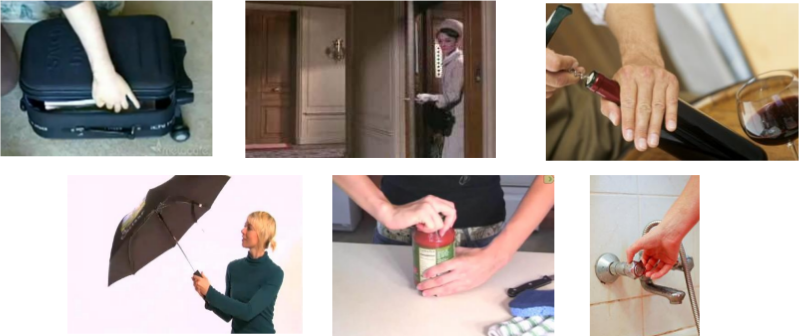
\includegraphics[scale=0.3]{open_example}
  \caption{Examples of ``Open'' action}
  \label{fig:open_example}

\end{figure}

In order to deal with those challenges, several standard action datasets have been created in order to develop
robust human action recognition systems and detection algorithms.
The first datasets included 1 actor performing using a static camera over homogeneous backgrounds.
Even though, those datasets helped us design the first action recognition algorithms, they were not able to deal with the above
challenges.
This lead us to design datasets containing more ambiguous videos, such as Joint-annotated Human Motion Database(JHMDB) (\cite{Kuehne11})
and UCF-101 (\cite{soomro2012ucf101}). These datasets contain only human actions, the second category presented above.

\subsection{JHMDB Dataset}
The JHMDB dataset (\cite{Jhuang:ICCV:2013}) is a fully annotated dataset for human actions and human poses. It is consisted of 21 action categories and 928
clips extracted from Human Motion Database (HMDB51) \cite{Kuehne11}. This dataset contains trimmed videos with duration between
15 to 40 frames. Each clip is annotated for each frame using a 2D pose and contains only 1 action.
In order to train our model for action localization, we modify 2D poses into 2D boxes containing the whole pose in each frame.
There are available 3 different splits for training data, proposed by the authors. We chose the first split which contains 660
videos for training set and 268 for validation . 

\subsection{UCF-101 Dataset}
The UCF-101 dataset (\cite{soomro2012ucf101}) contains 13320 videos from 101 action categories.
From those, for 24 classes and 3194 video spatiotemporal annotations are included. This means that there is a 2D bounding box surrounding the actor for each frame in which an action is taking place.
We separate dataset's videos into 2284 videos for training set and 910 for validation test according to the
first proposed training split. For training data, there are videos up to 641 frames, while in validation data max number of frames is 900.
Each video, both training and validation, is untrimmed, including sometimes more than 1 actions taking place simultaneously.
We took annotations from \cite{singh2016online} because those  proposed by the authors contain some mistakes.

\section{Motivation and Contributions}
The current achievements in Object Recognition Networks and in 3D Convolution Networks for Action Recognition have triggered us to try
to combine them in order to achieve state-of-the-art results for action localization. We introduce a new network structure inspired by
\cite{DBLP:journals/corr/HouCS17}, \cite{DBLP:journals/corr/abs-1712-09184},\cite{Ren:2015:FRT:2969239.2969250} and for implementation
by \cite{jjfaster2rcnn}.

Our contributions are the following:
\begin{enumerate}
\item We create a new framework for action localization extending the code taken from faster RCNN implementation. Based on the structure
  proposed by \cite{DBLP:journals/corr/HouCS17}, we modified it, using a 3D Resnet34 instead of C3D, which previous approach used.

\item Furthermore, we proposed our own TPN Network, a Network for proposing candidate action tubes give a small video segment.
  Following the approach \cite{DBLP:journals/corr/HouCS17} proposed, we firstly implement an architecture which uses
  cuboids as anchors, which then using a regressor it becomes a sequence of bounding boxes, likely to contain an action.
  We experiment with two candidate regressor's architecture and proposed and implement a 3D RoiAlign which uses trilinear
  interpolation for extracting each proposed action tube's activation maps. 
  Inspired by \cite{DBLP:journals/corr/abs-1712-09184}, we proposed and implement a TPN which uses predefined sequences of bounding
  boxes as 3D anchors. We proposed anchors that last equal with and less than video segment's duration in order our architecture to be able to
  perform temporal localization.  we explore two different regressors' architectures for better spatial precision using activation
  maps extracted from 2D RoiAlign, treating each frame separately.
\item Inspired by linking algorithm proposed by \cite{DBLP:journals/corr/HouCS17}, we introduce our own linking algorithm, which
  uses a combination of actioness and overlap scores in order to decide if 2 proposed action tubes would connect or not and some updatable lists.
  Our approach includes gathering all candidate action tubes whose score is bigger than a threshold, and use them as active action tubes for
  new possible connections. When the number of gathered active action tube is bigger than a threshold, we keep the k-best scoring action tubes
  and remove the rest.  We implement this algorithm using, also, CUDA code in order to calculate connection score faster. We proposed 3 versions of this algorithm:
  \begin{enumerate}
  \item An approach which uses an updatable scoring threshold, in order not to calculate unnecessary connection scores
  \item An approach which doesn't use an updatable scoring threshold, but it just updates ``active'' action tube more frequently.
  \item An approach which, also, uses NMS or softmax-NMS algorithms for getting wider action tube proposals.
  \end{enumerate}
  Also, we implement, from scratch, another connection algorithm proposed by \cite{DBLP:journals/corr/abs-1903-00304} and extending it in order to work for ToIs instead of frames, which they proposed.
  We modified our TPN structure in order to calculate progression and progress rate scores in order to calculate connection scores and generate candidate action tubes.
\item We experiment using several classifier in order to find the most suitable. We considered 2 feature maps extracted using 3D RoiAlign and proposed action tubes, without any other
  modification. Also, we explore the different ratios and number of groundtruth foreground tubes that should be used during training
  stage. Finally, we tried to perform only temporal localization using temporal information generated from proposed action tubes.
\end{enumerate}

\section{Thesis structure}
The rest of Thesis is organized as follows. Chapter 2 provides an general introduction to Machine Learning techniques currently used.
After that, we present the basic elements of object recognition systems and alongside with loss functions and evaluation metrics that
we used. Also, Chapter 2 presents an brief overview of literature on human action recognition and localization. Chapter 3 introduces the first basic element of our network, Tube Proposal Network (TPN), a network which proposes Tubes of Interest (ToIs), which are sequences of bounding boxes, with are likely to contain a performed action. Furthermore, it contains all the proposed architectures for achieving this.
Chapter 4 proposes algorithms for linking the proposed TOIs from every video segment and proposal performance is presented.
In Chapter 5, we present all the classification approaches we used for designing our architecture and some classification results.
Chapter 6 is used for conclusions, summary of our contribution alongside with possible future work.

% \end{document}

% \documentclass{report}

% \usepackage{subcaption} % package for subfigures
% \usepackage{hyperref}  % package for linking figures etc
% \usepackage{enumitem}  % package for description with bullets
% \usepackage{graphicx}  % package for importing images
% \usepackage{mathtools} % package for math equation
% \usepackage{mathrsfs}  % package for math font
% \usepackage{indentfirst} % package for getting ident after section or paragraph
% \usepackage{amssymb}
% % \usepackage{amsmath}
% \usepackage[
%     backend=bibtex,
%     citestyle=authoryear,
%     % citestyle=authoryear-comp,
%     % citestyle=authoryear-ibid,
%     bibstyle=numeric,
%     sorting=ynt,
%     % style=numeric,
%     % style=alphabetic ,
%   ]{biblatex}
 
%  \addbibresource{References}


% \setlength{\parindent}{2em} % how much indent to use when we start a paragraph

% \graphicspath{ {./theory/figures/} }       % path for images

% \begin{document}

\chapter{Background}


\section{Machine Learning}

\subsection{Introduction}
Machine Learning (ML) is a field which is raised out of Artificial Intelligence (AI). Applying AI, we wanted to build better and intelligent
machines. But except for mere tasks such as finding the shortest path between point A and B, we were unable to program more complex
and constantly evolving challenges. There was a realization that the only way to be able to achieve this task was to let machines learn
from themselves. This sounds similar to a child learning from its self. So machine learning was developed as a new capability for computers.
And now machine learning is present in so many segments of technology, that we don’t even realize it while using it. \par
Finding patterns in data on planet earth is possible only for human brains. Data being very massive and time taken to compute them made  Machine Learning take  action, in order to help people exploit them in minimum time. \\
There are three kinds of Machine Learning Algorithms :
 
\begin{enumerate}
\item Supervised Learning
\item Unsupervised Learning
\item Reinforcement Learning
\end{enumerate}

\subsubsection{Supervised Learning}
A majority of practical machine learning uses supervised learning. In supervised learning, the system tries to learn from the previous examples that are given. Speaking mathematically, supervised learning is where you have both input variables (\textit{x}) and output variables (\textit{Y}) and can use an algorithm to derive the mapping function from the input to the output. The mapping function is expressed as
$Y = f(x)$.
\begin{figure}[h]
  \centering
  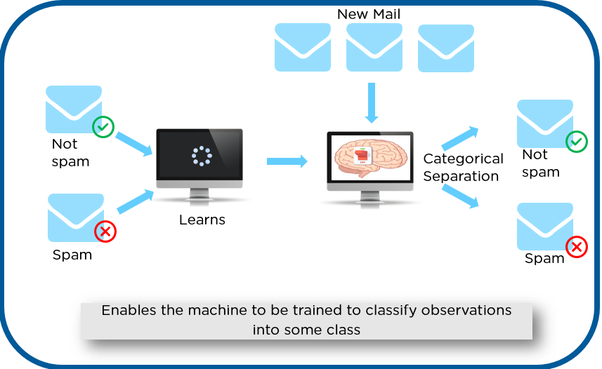
\includegraphics[scale=0.3]{supervised_leaning_example2}
  \caption{Example of supervised Learning}
  \label{fig:supervised_learning_example}
\end{figure}

As shown in Figure \ref{fig:supervised_learning_example}, we have initially taken some data and marked them as ‘Spam’ or ‘Not Spam’. This
labeled data is used by the training supervised model, in order to train the model. Once it is trained, we can test our model by testing it with some new mails and checking if the model is able to predict the right output. 

Supervised learning problems can be further divided into two parts, namely \textbf{classification}, and \textbf{regression}.
\begin{description}
\item[ Classification] : A classification problem is when the output variable is a category or a group, such as “black” or “white” or “spam” and “no spam”.
\item[ Regression ] :  A regression problem is when the output variable is a real value, such as “Rupees” or “height.”
\end{description}
Some Supervised learning algorithms include:
\begin{itemize}
\item Decision trees
\item Support-vector machine
\item Naive Bayes classifier
\item k-nearest neighbors
\item linear regression
\end{itemize}

\subsubsection{Unsupervised Learning}

In unsupervised learning, the algorithms are left to themselves to discover interesting structures in the data. Mathematically, unsupervised
learning is when you only have input data (\textit{X}) and no corresponding output variables. This is called unsupervised learning because
unlike supervised learning above, there are no given correct answers and the machine itself finds the answers.
\begin{figure}[h]
  \centering
  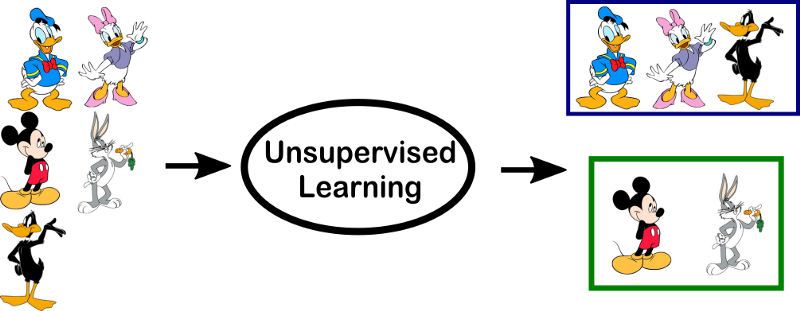
\includegraphics[scale=0.3]{unsupervised_learning_example}
  \caption{Example of unsupervised Learning}
  \label{fig:unsupervised_learning_example}
\end{figure}
In Figure \ref{fig:unsupervised_learning_example}, we have given some characters to our model which are ‘Ducks’ and ‘Not Ducks’. In our
training data, we don’t provide any label to the corresponding data. The unsupervised model is able to separate both the characters by
looking at the type of data and models the underlying structure or distribution in the data in order to learn more about it. Unsupervised
learning problems can be further divided into \textbf{association} and \textbf{clustering} problems.

\begin{description}
\item[ Association] : An association rule learning problem is where you want to discover rules that describe large portions of your data, such as “people that buy X also tend to buy Y”.
\item[ Clustering] : A clustering problem is where you want to discover the inherent groupings in the data, such as grouping customers by purchasing behavior.
\end{description}

\subsubsection{Reinforcement Learning}
A computer program will interact with a dynamic environment in which it must perform a particular goal (such as playing a game with an
opponent or driving a car). The program is provided feedback in terms of rewards and punishments as it navigates its problem space. 
Using this algorithm, the machine is trained to make specific decisions. It works this way: the machine is exposed to an environment
where it continuously trains itself using trial and error method.
\begin{figure}[h]
  \centering
  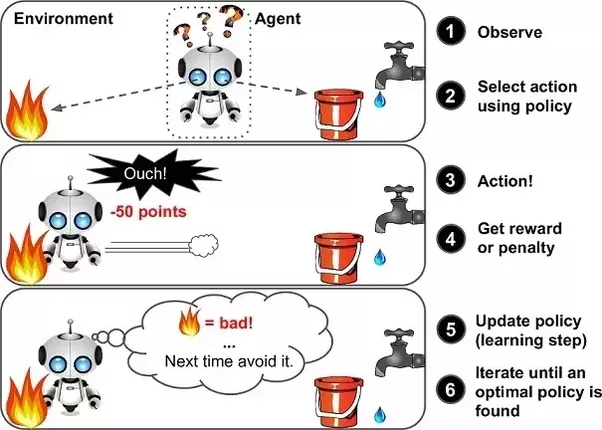
\includegraphics[scale=0.3]{reinforment_learning_example}
  \caption{Example of Reinforcement Learning}
  \label{fig:reinforment_learning_example}
\end{figure}
In Figure \ref{fig:reinforment_learning_example}, we can see that the agent is given 2 options i.e. a path with water or a path with fire. A reinforcement algorithm
works on reward a system i.e. if the agent uses the fire path then the rewards are subtracted and agent tries to learn that it should avoid
the fire path. If it had chosen the water path or the safe path then some points would have been added to the reward points, the agent then
would try to learn what path is safe and what path isn’t

\subsection{Neural Networks}
Neural Networks are a class of models within the general machine learning literature. Neural networks are a specific set of algorithms that
have revolutionized the field of machine learning. They are inspired by biological neural networks and the current so called deep neural
networks have proven to work quite very well. Neural Networks are themselves general function approximations, that is why they can be applied
to literally almost any machine learning problem where the problem is about learning a complex mapping from the input to the output space.

\subsection{A single Neuron}
The basic unit of computation in a neural network is the neuron, often called a \textbf{node} or \textbf{unit}. It receives input from some
other nodes, or from an external source and computes an output. In purely mathematical terms, a neuron in the machine learning world is a
placeholder for a mathematical function, and its only job is to provide an output by applying the function on the inputs provided.
Each input has an associated weight (\textit{w}), which is assigned on the basis of its relative importance to other inputs. The node applies
a function \textit{f  (defined below)} to the weighted sum of its inputs as shown in Figure \ref{fig:Perceptron}.
\begin{figure}[h]
  \centering
  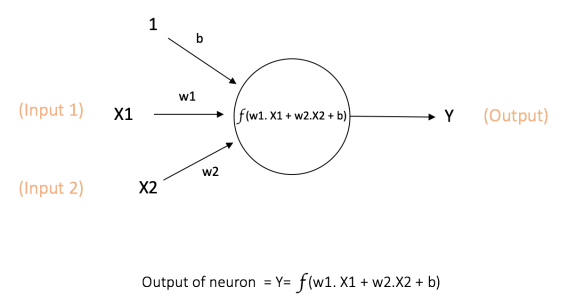
\includegraphics[scale=1.0]{perceptron}
  \caption{An example of a single Neuron}
  \label{fig:Perceptron}
\end{figure}
The network takes numerical inputs \textit{X1} and \textit{X2} and has weights \textit{w1} and \textit{w2} associated with those inputs.
Additionally, there is another \textit{input 1} with weight \textit{b} (called \textit{Bias}) associated with it. The main function of Bias is to provide every node with a trainable constant value (in addition to the normal inputs that the node receives). The output Y from the neuron
is computed as shown in the Figure \ref{fig:Perceptron}. The function \textit{f} is non-linear and is called \textbf{Activation Function}. The
purpose of the activation function is to introduce non-linearity into the output of a neuron. This is important because most real world data
are non linear and we want neurons to learn these non-linear representations.
\subsubsection{Activation Functions} 
Every activation function (or non-linearity) takes a single number and performs a certain fixed mathematical operation on it. There are
several activation functions:
\begin{description}
\item[ Sigmoid ] : takes a real-valued input and squashes it to range between 0 and 1. Its formula is:
  \[ \sigma(x) = \frac{1}{1 + e^{-x} } \]
  It is easy to understand and apply but it has major reasons which have made it fall out of popularity:
  \begin{itemize}
  \item Vanishing gradient problem
  \item Its output isn’t zero centered. It makes the gradient updates go too far in different directions.
  \item Sigmoids saturate and kill gradients.
  \item Sigmoids have slow convergence.
  \end{itemize}

\item [ Tanh ] : takes a real-valued input and squashes it to the range [-1, 1]. Its formula is:
  \[ tanh(x) = 2 \sigma(2x) -1 \]
  Now it’s output is zero centered because its range in between -1 to 1. Hence optimization is easier in this method and  in practice it is always preferred over Sigmoid function . But still it suffers from Vanishing gradient problem.

\item[ Re-LU ]: Re-LU stands for \textit{Rectified Linear Unit}. It takes a real-valued input and thresholds it at zero (replaces negative values with zero). So its formula is:
  \[ f(x) = max(0,x) \]
  It has become very popular in the past couple of years. It was recently proved that it had 6 times improvement in convergence from Tanh
  function. Seeing the mathematical form of this function we can see that it is very simple and efficient . A lot of times in Machine
  learning and computer science we notice that most simple and consistent techniques and methods are only preferred and are best.
  Hence it avoids and rectifies vanishing gradient problem . Almost all deep learning Models use ReLu nowadays.
\end{description}

Figure \ref{fig:Activation}  show each of the above activation functions.
\begin{figure}[h]
  \centering
  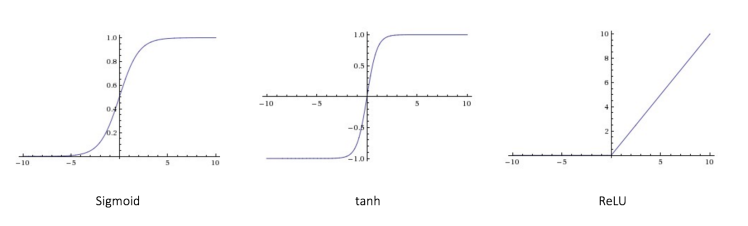
\includegraphics[scale=1.0]{activation_figures}
  \caption{Plots of Activation functions}
  \label{fig:Activation}
\end{figure}

\subsubsection{Feed-forward Neural Network}
Till now we have covered neuron and activation functions which together for the basic building blocks of any neural network. The feedforward
neural network was the first and simplest type of artificial neural network devised. It contains multiple neurons (nodes) arranged in layers.
A layer is nothing but a collection of neurons which take in an input and provide an output. Inputs to each of these neurons are processed
through the activation functions assigned to the neurons. Nodes from adjacent layers have connections or edges between them. All these connections have weights associated with them.
\begin{figure}[h]
  \centering
  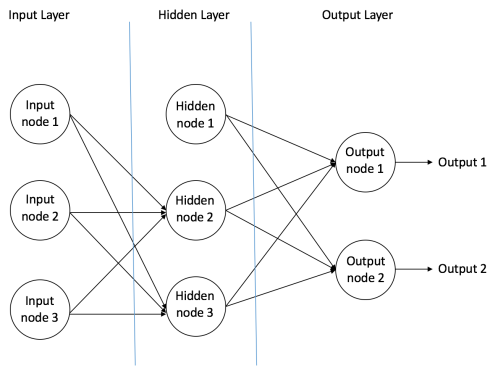
\includegraphics[scale=1.0]{feedforwardnetwork}
  \caption{An example of a Feedforward Neural Network}
  \label{fig:feedforwardnetwork}
\end{figure}
An example of a feedforward neural network is shown in Figure \ref{fig:feedforwardnetwork}. A feedforward neural network can consist of three types of nodes:
\begin{description}
\item[ Input Nodes ] The Input nodes provide information from the outside world to the network and are together referred to as the
  “Input Layer”. No computation is performed in any of the Input nodes – they just pass on the information to the hidden nodes.
\item[  Hidden Nodes ]  The Hidden nodes have no direct connection with the outside world (hence the name “hidden”). They perform
  computations and transfer information from the input nodes to the output nodes. A collection of hidden nodes forms a “Hidden Layer”.
  While a feedforward network will only have a single input layer and a single output layer, it can have zero or multiple Hidden Layers.
\item [ Output Nodes ] The Output nodes are collectively referred to as the “Output Layer” and are responsible for computations and
  transferring information from the network to the outside world.
\end{description}

In a feedforward network, the information moves in only one direction – forward – from the input nodes, through the hidden nodes (if any)
and to the output nodes. There are no cycles or loops in the network (this property of feed forward networks is different from Recurrent
Neural Networks in which the connections between the nodes form a cycle). Another important point to note here is that each of the hidden
layers can have a different activation function, for instance, hidden layer1 may use a sigmoid function and hidden layer2 may use a ReLU,
followed by a Tanh in hidden layer3 all in the same neural network. Choice of the activation function to be used again depends on the
problem in question and the type of data being used.

\subsection {2D Convolutional Neural Network}
A Convolutional Neural Network (ConvNet/CNN) is one of the variants of neural networks used heavily in the field of Computer Vision. It
derives its name from the type of hidden layers it consists of. The hidden layers of a CNN typically consist of convolutional layers, pooling
layers, fully connected layers, and normalization layers. Here it simply means that instead of using the normal activation functions defined
above, convolution and pooling functions are used as activation functions.
It can take in an input image, assigning importance (learning weights and biases) to various aspects/objects in the image and be able to
differentiate one from the other. The pre-processing required in a ConvNet is much lower as compared to the other classification algorithms.
While in primitive method filters are hand-engineered, with enough training, ConvNets have the ability to learn these filters/characteristics.

The architecture of a ConvNet is analogous to that of the connectivity pattern of Neurons in the Human Brain and was inspired by the
structure of the Visual Cortex. However, most ConvNets consist mainly in 2 parts:
\begin{description}[font=$\bullet$\scshape\bfseries]
\item [ Feature extractor] : \\
  This part of the network takes as input the image and extract features that are meaningful for its classification. It amplifies aspects
  of the input that are important for discrimination and suppresses irrelevant variations. Usually, the feature extractor consists of
  several layers. For instance, an image which could be seen as an array of pixel values. The first layer often learns representation
  that represent the presence or absence of edges at particular orientations and locations in the image. The second layer typically
  detects motifs by spotting particular arrangements of edges, regardless of small variations in the edge positions. Finally, the third
  may assemble motifs into larger combinations that correspond to paths of familiar objects, and subsequent layers would detect objects
  as combinations of these parts.
  
\item [ Classifier ] : \\
  This part of the network takes as input the previously computed features and use them to predict the correct label.
\end{description}

\begin{figure}[h]
  % 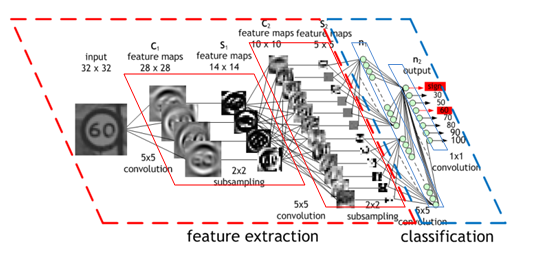
\includegraphics[scale=0.7]{convolutional_neural_network_structure} \]
  \centering
  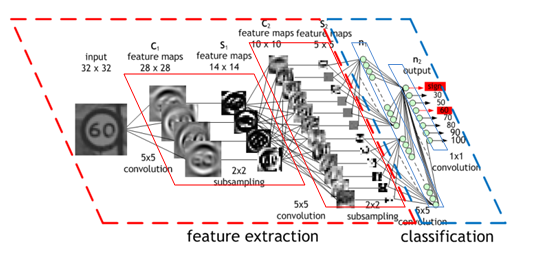
\includegraphics[scale=0.7]{convolutional_neural_network_structure}
  \caption{Typical structure of a ConvNet}
\end{figure}
\paragraph{Convolutional Layers}
In order to extract such features, ConvNets use 2D convolution operations. These operations take place in convolutional layers. Convolutional
layers consist of a set of learnable filters. Every filter is small spatially (along width and height), but extends through the full depth of
input. During forward pass, we slide (more precisely, convolve) each filter across the width and height of the input volume and compute dot
products between the entries of the filter and the input at any position (as Figure \ref{fig:conv_example} shows). The objective of the
Convolution Operation is to extract the high-level features such as edges, from the input image. ConvNets need not be limited to only one
Convolutional Layer. Conventionally, the first ConvLayer is responsible for capturing the Low-Level features such as edges, color, gradient
orientation, etc. With added layers, the architecture adapts to the High-Level features as well, giving us a network which has the wholesome
understanding of images in the dataset, similar to how we would.

\begin{figure}[h]
  \centering
  \begin{minipage}[b]{0.4\textwidth}
    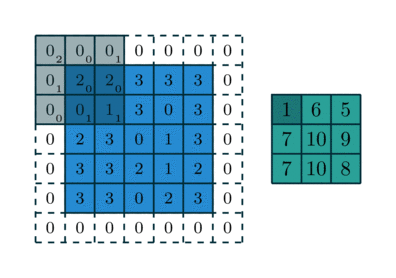
\includegraphics[width=\textwidth]{conv_1}
  \end{minipage}
  \hfill
  \begin{minipage}[b]{0.4\textwidth}
    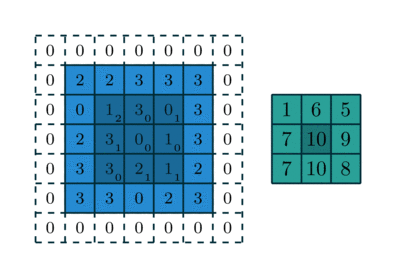
\includegraphics[width=\textwidth]{conv_2}
  \end{minipage}
  \caption{Convolution with kernel of 3, stride of 2 and padding of 1}
  \label{fig:conv_example}
\end{figure}
\paragraph{Pooling Layers}
Pooling Layers are also referred as downsampling layers and are used to reduce the spatial dimensions, but not depth, on a convolution neural network.
The intuitive reasoning behind this layer is that once we know that a specific feature is in the original input volume (there will be a high activation value),
its exact location is not as important as its relative location to the other features. The main advantages of pooling layer are:

\begin{itemize}
\item We gain computation performance since the amount of parameters is reduce.
\item Less parameters also means we deal with overfitting situations.
\end{itemize}

The pooling operation is specified, rather than learned. Two common functions used in the pooling operation are:
\begin{description}
\item[ Average Pooling ] Calculate the average value for each patch on the feature map.
\item[ Maximum Pooling (or Max Pooling) ] Calculate the maximum value for each patch of the feature map.
\end{description}

\begin{figure}[h]
  \centering
  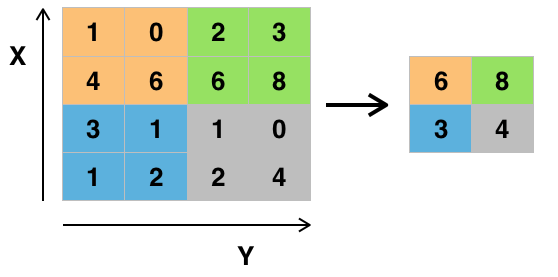
\includegraphics[scale=0.35]{max_pooling}
  \caption{Example of Max pooling operation with a 2x2 filter  and stride of 2}
  \label{fig:pooling_eg}
\end{figure}

\subsection{3D Convolutional Neural Network}
Traditionally, ConvNets are targeting RGB images (3 channels). The goal of 3D CNN is to take as input a video and extract features from it.
When ConvNets extract the graphical characteristics of a single image and put them in a vector (a low-level representation), 3D ConvNets
extract the graphical characteristics of a set of images. 3D CNNs takes in to account a temporal dimension (the order of the images in the
video). From a set of images, 3D CNNs find a low-level representation of a set of images, and this representation is useful to find the
right label of the video (a given action is performed). In order to extract such features, 3D ConvNets  use 3D convolution operations, whose kernel
shape for a 3D Convolution is specified along 3 dimensions. When thinking about the convolution operation in terms of a kernel sliding
across a multidimensional input array, for a 3D Convolution, the kernel slides in 3 directions
Their output shape is a 3 dimensional volume space such as cube or cuboid.

\begin{figure}[h]
  % 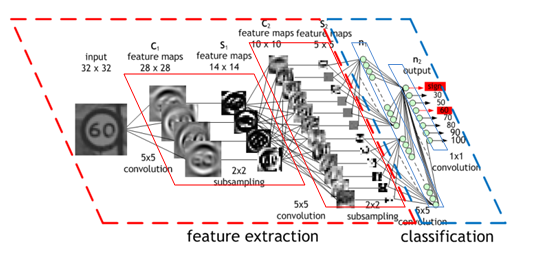
\includegraphics[scale=0.7]{convolutional_neural_network_structure} \]
  \centering
  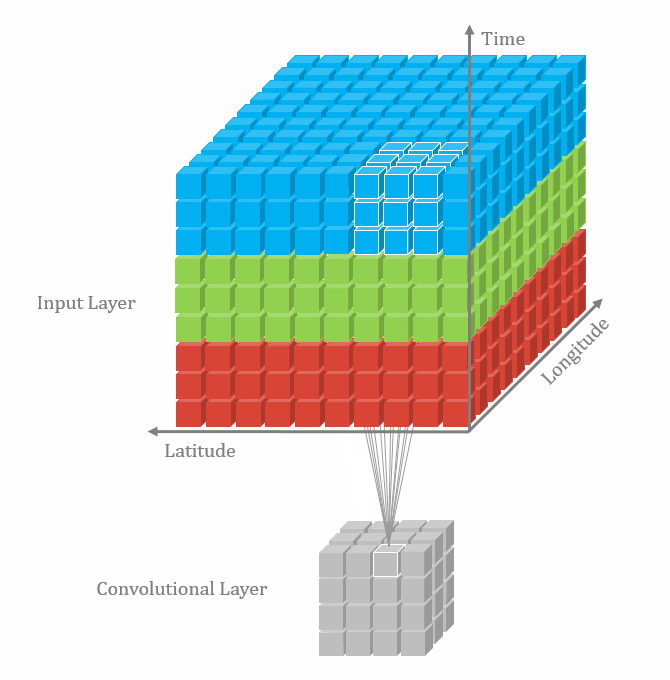
\includegraphics[scale=0.3]{3d_conv}
  \caption{3D Convolution operation}
\end{figure}

Also, such 3D relationship is important for some applications, such as in 3D segmentations / reconstructions of biomedical imagining,
e.g. CT and MRI where objects such as blood vessels meander around in the 3D space.
% There are several existing approaches to tackle the video classification. This is a nonexaustive list of existing approaches:
% \begin{description} [font=$\bullet$\scshape\bfseries]
% \item[ ConvNets + LSTM cell] : Extract features from each frame with a ConvNet, passing the sequence to an RNN
% \item[ Temporal Relation Networks] : Extract features from each frame with a ConvNet and pass the sequence to an MLP
% \item[ Two-Stream Convolutional Networks] : Use 2 CNN, 1 spatial stream ConvNet which process one single frame at a time, and 1 Temporal stream ConvNet which process multi-frame optical flow
% \end{description}

\section{Object Detection}
Within the field of Deep Learning, the sub-discipline called ``Object Detection'' involves processes such as identifying the objects through a picture, video or a webcamera feed. The challenge of detecting all objects existing in image in counterpart of action localization in videos and
a lot of object detection techniques are used in action localization architectures, so it is worth presenting it.
Object Detection methods are used almost everywhere these days. The use cases are endless such as Tracking objects, Video surveillance, Pedestrian detection etc. 
An object detection model is trained to detect the presence and location of multiple classes of objects. For example, a model might be trained with images that
contain various pieces of fruit, along with a label that specifies the class of fruit they represent (e.g. an apple, a banana, or a strawberry),
and data specifying where each object appears in the image.

The main process followed by most of CNN for Object Detection is:
\begin{enumerate}
\item Firstly, we do feature extraction using as backbone network, the first Convolutional Layers of a known pre-trained CNN such
  as AlexNet, VGG, ResNet etc.
\item Then, we propose regions of interest (ROI) in the image. These regions contain possibly an object, which we are looking for.
\item Finally, we classify each proposed ROI.
\end{enumerate}

\subsection{ Region Proposal Network}

From the 3 above steps, the 2nd step is considered to be very important. That is because, in this step, we should choose regions of
the image, which will be classified. Poor choice of ROIs means that the CNN will pass by some object that are located in the image,
because, they were not be proposed to be classified.

\begin{figure}[h]
  \centering
  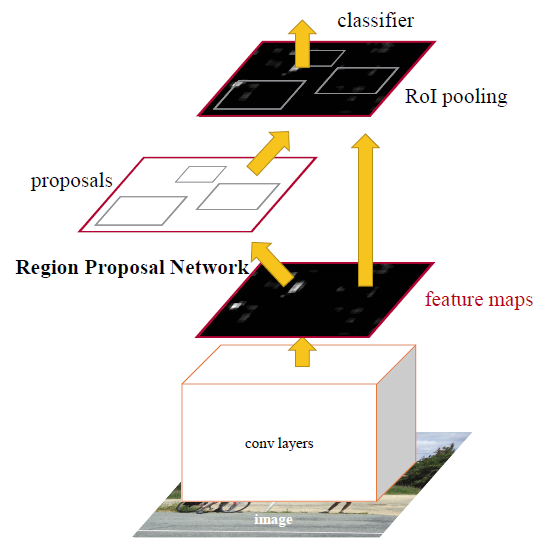
\includegraphics[scale=0.3]{RPN_structure}
  \caption{ Region Proposal Network's structure}
  \label{fig:rpn_structure}
\end{figure}

The first Object-Detection CNNs use several algorithms for proposing ROIs. For example, R-CNN(\cite{DBLP:journals/corr/GirshickDDM13}),
and Fast R-CNN(\cite{Girshick:2015:FR:2919332.2920125}) used Selective Search Algorithm for extracting ROIs.
One of novelties introduced by the Faster R-CNN(\cite{Ren:2015:FRT:2969239.2969250}) is \textbf{Region Proposal Network} (RPN). Its
function is to propose ROIs and its structure can be shown in \ref{fig:rpn_structure}. As we can see, RPN is consisted of:
\begin{itemize}
\item 1 2D Convolutional Layer
\item 1 score layer 
\item 1 regression layer
\end{itemize}

Before describing RPN's function, we introduce another basic element of RPN which is its \textbf{anchors}. Anchors are predefined boxes used for extracting ROIs. In figure \ref{fig:anchors} is
depicted an example of some anchors
\begin{figure}[h]
  \centering
  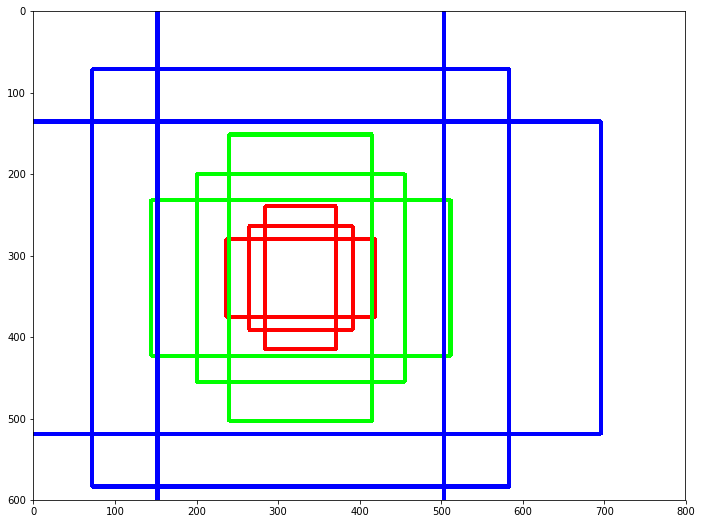
\includegraphics[scale=0.3]{anchors}
  \caption{ Anchors for pixel (320,320) of an image (600,800) }
  \label{fig:anchors}
\end{figure}

For each feature map's pixel corresponds \textbf{k (k=9)} anchors (3 different scales and 3 different ratios 1:1, 1:2, 2:1). \par
So, RPN's procedure is:
\begin{enumerate}
\item RPN gets as input feature maps extracted from the backbone CNN.
\item Then it performs 2D convolution over this input and passes the output to its scoring layer and regression layer.
\item Scoring layer produces confidence score of existing an object in each anchor's area. On the other hand, regression layer outputs 4k displacements, 4 for each anchor. Finally, we keep as output only the \textit{ n-best scoring} anchors.
\end{enumerate}

\subsection{Roi Align}

The biggest problem facing Object Detection Networks is the need for fixed input size. Classification networks require a fixed input size, which
is easy for image classification because it is handled by resizing the input image. However, in object recognition architectures, each proposal has a different size
and shape. This creates the need for converting all proposals to a fixed shape. At Fast-RCNN(\cite{Girshick:2015:FR:2919332.2920125}) and
Faster-RCNN(\cite{Ren:2015:FRT:2969239.2969250}) methods, this operation happens by applying Roi Pooling. However, this wrapping is digitalized because
the cell boundaries of the target feature map are forced to realign with the boundary of the input feature maps as shown in Figure \ref{fig:roi_pooling_align_1}
(the top left diagram). As a result, each target cells may not be in the same size (Figure \ref{fig:roi_pooling_align_2}).


\begin {figure}[h]

  \begin{subfigure}{0.35\textwidth}
    \centering
    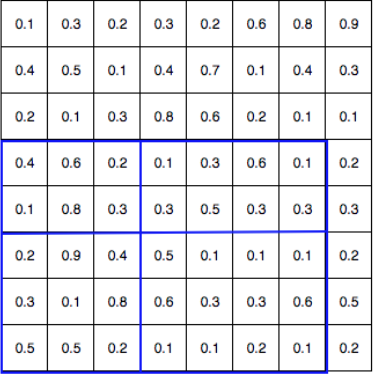
\includegraphics[scale=0.3]{roi_align_1}
    \caption{}
    \label{fig:roi_pooling_align_1}
  \end{subfigure}
  \hfill
  \begin{subfigure}{0.35\textwidth}
    \centering
    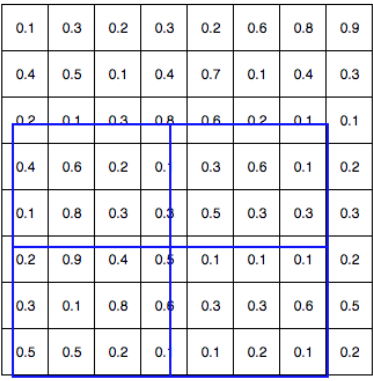
\includegraphics[scale=0.3]{roi_al_3}
    \caption{}
    \label{fig:roi_pooling_align_3}
  \end{subfigure}
  \hfill
  \begin{subfigure}{0.35\textwidth}
    \centering
    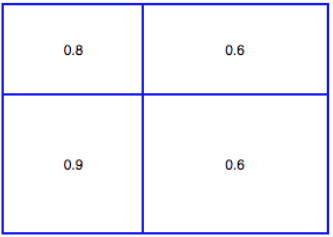
\includegraphics[scale=0.3]{roi_al_2}
    \caption{}
    \label{fig:roi_pooling_align_2}
  \end{subfigure}
  \hfill
  \begin{subfigure}{0.35\textwidth}
    \centering
    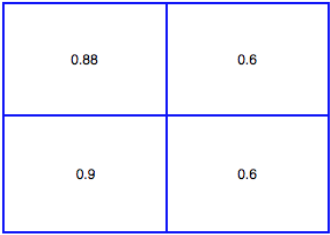
\includegraphics[scale=0.3]{roi_al_4}
    \caption{}
    \label{fig:roi_pooling_align_4}
  \end{subfigure}
  \caption{Roi Pooling and Roi Align examples}
  \label{fig:roi_pooling_align}
\end{figure}

On the other hand, Mask-RCNN (\cite{DBLP:journals/corr/HeGDG17}) introduced Roi Align operation. Roi Align avoids digitalizing
the boundary of the cells as shown in Figure \ref{fig:roi_pooling_align_3}, and achieves to make every target cell to have the same size
according to Figure \ref{fig:roi_pooling_align_4}. In order to calculate feature maps values, Roi Align uses bi-linear interpolation as
shown in Figure \ref{fig:roi_align_2}. This means that we calculate the value of the desired bins according to their neighbors'.

\begin{figure}[h]
  \centering
  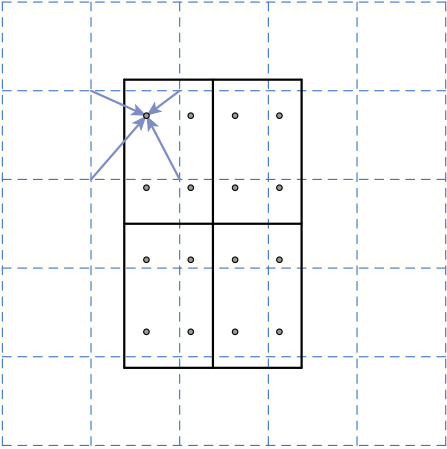
\includegraphics[scale=0.35]{roi_align_2}
  \caption{Example of bi-linear interpolation for calculation Roi Align's final feature map}
  \label{fig:roi_align_2}
\end{figure}

\subsection{Non-maximum suppression (NMS) algorithm}

Another problem that object detection networks face is that neighbor bounding boxes have similar scores to some extent. Most object
detection systems employ a sliding window or a Region Proposal Network for proposing areas in the image that is likely to contain an
object. These techniques, which return several areas in the images, achieve high recall performance. However, in these approaches,
more that 1 proposal may be related with only one ground-truth object coordinates. This situation creates
the need for choosing the best proposals, because, alternatively, hundreds of unnecessary proposals will be classified. For that
reason, Non-Maximum Suppression (NMS) algorithm was proposed for filtering these proposals base on some criteria. NMS gets as input
a list of proposal bounding boxes B, their corresponding confidence score S and an overlap threshold N and return as output
a list of the final filtered proposals D. NMS algorithm's steps are:
\begin{enumerate}
  
\item Initialize an empty list D. Select the proposal with the highest confidence score, remove it from B and add it to D.
\item Calculate the overlap score between this proposal and all the other proposals. For all the proposals that their overlap
  score is bigger than N, remove from B.
\item From the remaining proposals, picked again the one with the highest score and remove it from B.
\item Repeat steps 2 and 3 until no more proposals are left in list B.
\end{enumerate}

The aforementioned algorithm shows that the whole process depends mostly on a single threshold value.  So that makes the selection
of threshold a crucial factor for the performance of the model. In some situations, bad choice of the threshold may make the network
to remove bounding boxes with good confidence score, if there are side by side. Figure \ref{fig:nms_eg} shows a situation like this,
where red and blue boxes will be removed because of the presence of the black box.
\begin{figure}[h]
  \centering
  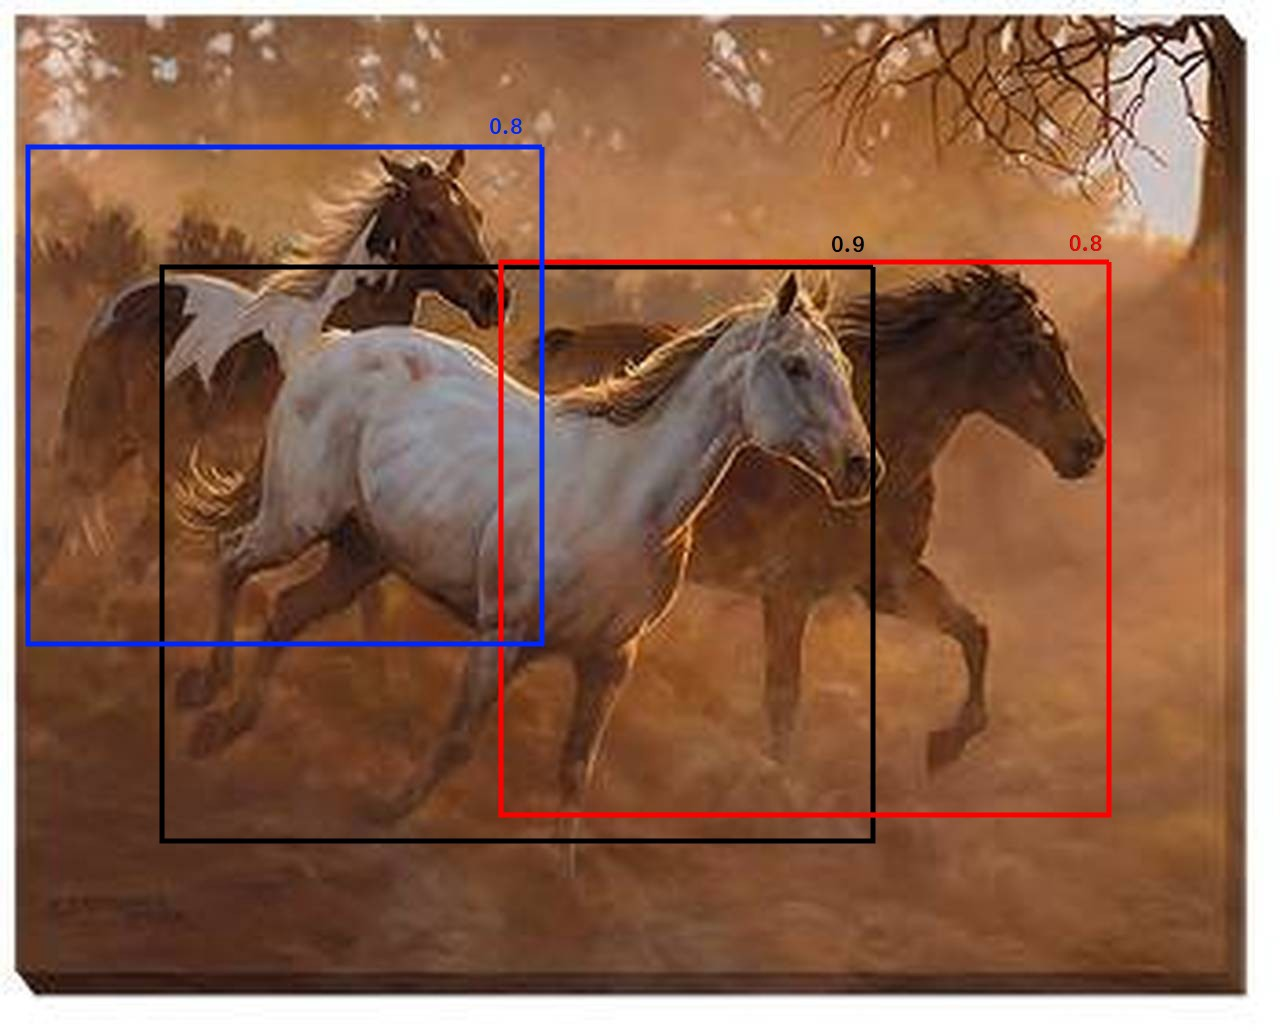
\includegraphics[scale=0.2]{soft_nms.jpeg}
  \caption{Example of a situation where NMS algorithm will remove good proposals}
  \label{fig:nms_eg}
\end{figure}

\subsubsection{Soft NMS}
A simple and efficient way to deal the aforementioned situation is to use Soft-NMS algorithm, which is presented in \cite{DBLP:journals/corr/BodlaSCD17}.
Soft-NMS algorithm is based on the idea of
reducing confidence score of the proposals proportional to their overlap score, instead of completely removing them.
The score calculation follows the formula 
\[ s_i = \begin{dcases}
    s_i, & overlapscore(M, b_i) < N_t \\
    s_i(1-overlapscore(M, b_i)), & overlapscore(M, b_i) \ge N_t
    \end{dcases}
    \]

    where $s_i$ is the score of proposal $i$, $b_i$ is the box coordinates of proposal $i$, $M$ is the coordinates of
    the box with the maximum confidence and $N_t$ is the overlap threshold. Let's, again, consider as input a list of
    proposal bounding-boxes B, their corresponding confidence score S and as output a list of proposals D. Soft-NMS algorithm includes the following steps:

\begin{enumerate}
  
\item Select the proposal with the highest confidence score, remove it from B and add it to D.
\item Calculate the overlap score between this proposal and all the other proposals. For all the proposals that their overlap
  score is bigger than N, recalculate their confidence score according to previous formula.
\item From the remaining proposals, picked again the one with the highest score and remove it from B.
\item Repeat steps 2 and 3 until no more proposals are left in list B.
\end{enumerate}
    
    
\section{Losses and Metrics}
In order to train our model and check its performance, we use some known Loss functions and Metrics used in Object Detection systems.
\subsection{Losses}
For training our network, we use \textbf{Cross Entropy Loss} for classification layers and \textbf{smooth L1-loss} for bounding box regression
in each frame and their diagram is show at Figure \ref{fig:cross_l1}.
\subsubsection{Cross Entropy Loss}
Cross-entropy loss, or log loss, measures the performance of a classification model whose output is a probability value between 0 and 1. \par
Entropy is the measure of uncertainty associated with a given distribution \textit{q(y)} and its formula is: 
\[ H = -\sum_{i=1}^n p_i \cdot \log p_i \]
Intuitively, entropy tells us how ``surprised'' we are when some event E happened. When we are sure about an event E to happened ($ p_E = 1$)
we have 0 entropy (we are not surprised) and vise versa. \par
On top of that, let's assume that we have 2 distributions, one known (our network's distribution) \textit{p(y)} and one unknown (the actual
data's distribution) \textit{q(y)}. Cross-entropy tells us how accurate is our known distribution in predicting the unknown distribution's
results. Respectively, Cross-entropy measures how accurate is our model in predicting the test data. Its formula is:
\[ H_p(q) = - \sum_{c=1}^C q(y_c) \cdot log(p(y_c)) \]

\subsubsection{Smooth L1-loss}

Smooth L1-loss can be interpreted as a combination of L1-loss and L2-loss. It behaves as L1-loss when the absolute
value of the argument is high, and it behaves like L2-loss when the absolute value of the argument is close to zero.
It is usually used for doing box regression on some object detection systems like Fast-RCNN(\cite{Girshick:2015:FR:2919332.2920125}),
Faster-RCNN(\cite{Ren:2015:FRT:2969239.2969250}) and it is less sensitive to outliers according according to \cite{Girshick:2015:FR:2919332.2920125}.
As shown in \cite{Girshick:2015:FR:2919332.2920125}, its formula is:

\[ smooth_{L1}(x) = \begin{dcases}
    0.5x^2 & \text{ if } x < 1 \\
    |x| - 0.5 & \text{otherwise}
  \end{dcases}\]

It is similar to Huber loss whose formula is:

\[
L_{\delta}(x) = \begin{dcases}
    \frac{1}{2}a^2 & \text{ for } |a| \le \delta \\
\delta(|a| - \frac{1}{2}\delta), & \text{otherwise}
\end{dcases}
\]

if we set $\delta $ parameter equal 1. \par

Smooth L1-loss combines the advantages of L1-loss (steady gradients for large values of \textit{x}) and L2-loss (less oscillations during
updates when \textit{x} is small). Figure \ref{fig:smooth_l1} shows a comparison between L1-norm, L2-norm  and smooth-L1 .

\begin{figure}[h]
  \centering
  \begin{subfigure}{0.49\textwidth}
    % \fbox{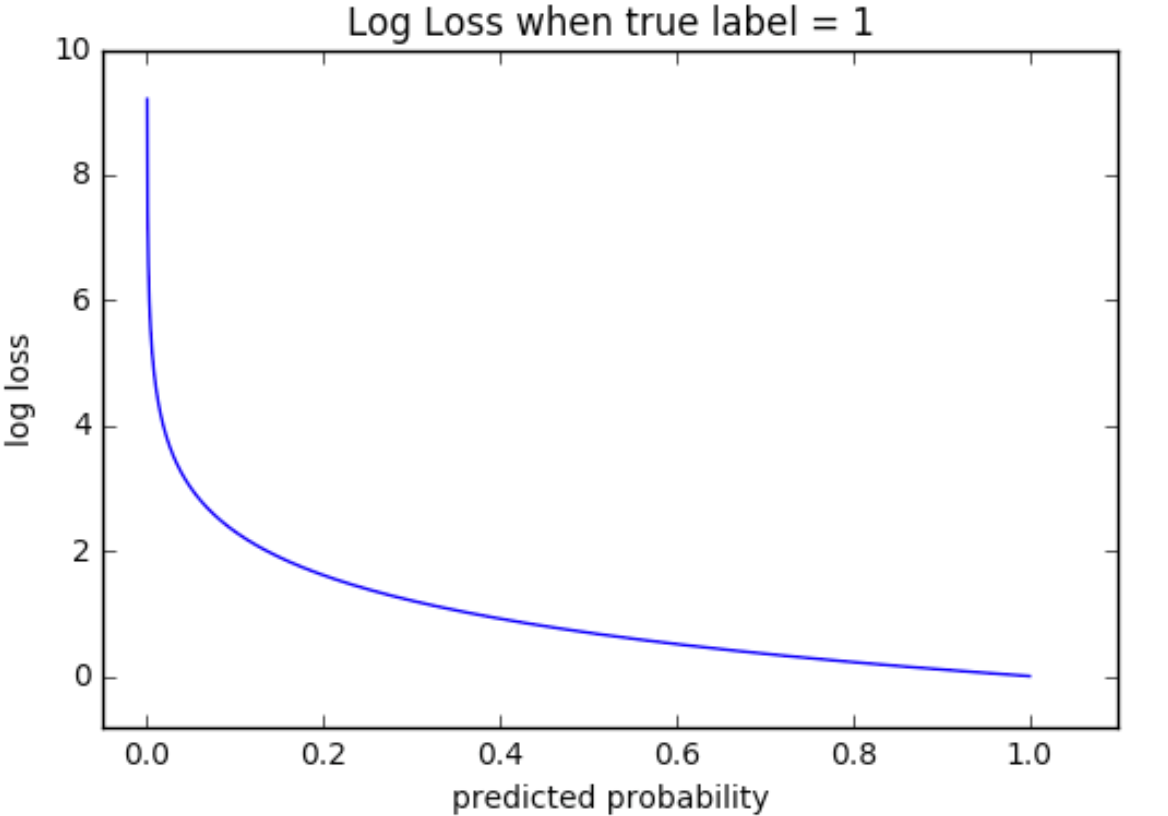
\includegraphics[width=\textwidth]{c_entropy}}
    % 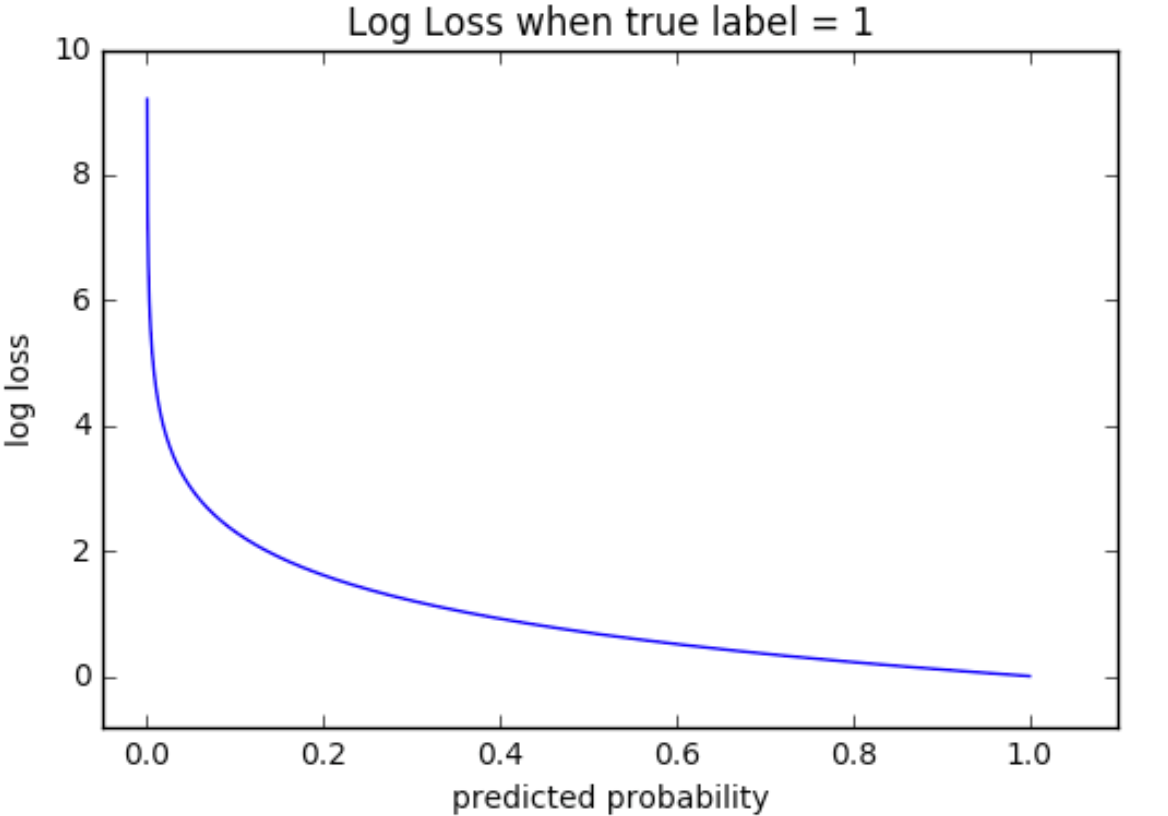
\includegraphics[width=\textwidth]{c_entropy}
    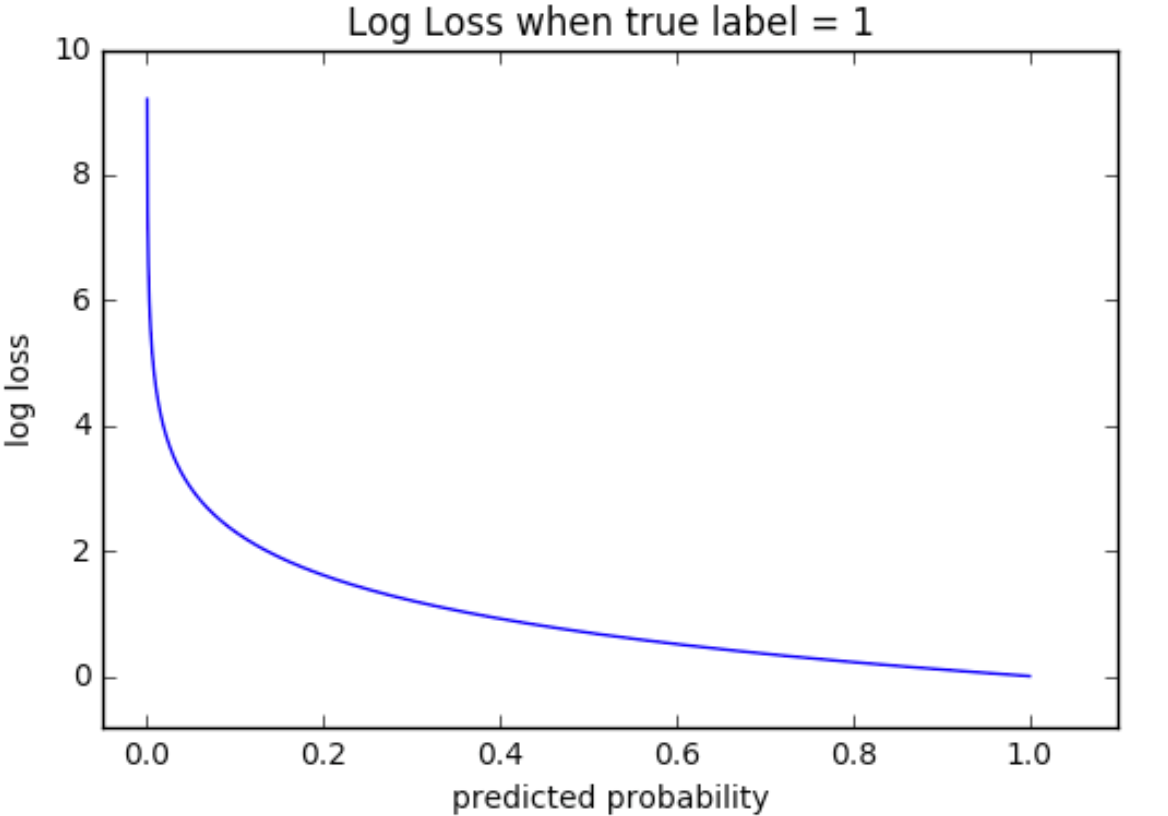
\includegraphics [width=7.0cm,height=4.5cm]{c_entropy}
      \caption{}
      \label{fig:cross_entropy}

  \end{subfigure}
  \hfill
  \begin{subfigure}{0.49\textwidth}
% \fbox{    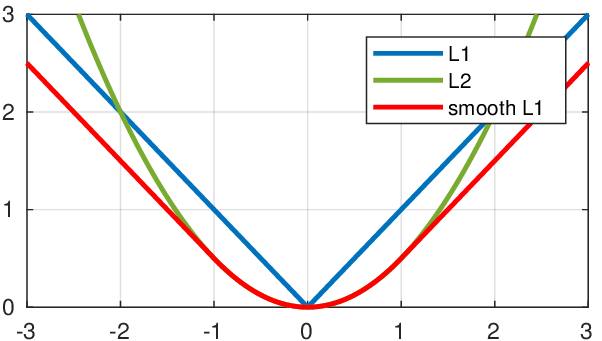
\includegraphics [width=5.5cm,height=3.8cm]{smooth_l1}}
    \includegraphics[width=\textwidth]{smooth_l1}
    % \includegraphics [width=6.0cm,height=4cm]{smooth_l1}
    % \includegraphics[width=\textwidth]{smooth_l1}
      \caption{}
      \label{fig:smooth_l1}
  \end{subfigure}

  \caption{ (\subref{fig:cross_entropy}) and (\subref{fig:smooth_l1})  show the behavior of cross-entropy loss and smooth-L1 respectively.}
  \label{fig:cross_l1}%
\end{figure}

\subsection{Metrics}
Evaluating our machine learning algorithm is an essential part of any project. The way we choose our metrics influences how the performance
of machine learning algorithms is measured and compared.
They influence how to weight the importance of different characteristics in the results and finally,
the ultimate choice of classification algorithm. Most of the times we use classification accuracy
to measure the performance of our model, however it is not enough to truly judge our model. \par
At first, we introduce some basic evaluation metrics in order,then, to present those we use for our assessment.

\subsubsection{Intersection over Union}
The first and most important metric that we use is Intersection over Union (IoU). IoU  measures the overlap between 2 boundaries.
It is usually used in Object Recognition Networks in order to define how good overlap a predicted bounding box  with the actual
bounding box as shown in Figure \ref{fig:iou_fig}. We predefine an IoU threshold (say 0.5) in classifying whether the prediction is a true positive or a false positive.
\begin{figure}[h]
  \centering
  \includegraphics[scale=0.55]{iou}
  \caption{Example of IoU scoring policy}
  \label{fig:iou_fig}
\end{figure}

Intersection over Union is defined as:
\[ IoU = \frac{\text{area of overlap}}{\text{area of union}} \]
In Figure \ref{fig:iou_fig}, spatial IoU between 2 bounding boxes, $(x_1,y_1,x_2,y_2)$ and $(x_3,y_3,x_4,y_4)$,is presented, which means IoU metric is implemented for x-y dimensions.
Area of overlap and area of union can be defined as:
\[\text{ Area of overlap } = \lVert( min(x_2,x_4) - max(x_1,x_3), min(y_2,y_4)- max(y_1,y_3) )\rVert\]
\[\text{ Area of union  }  = \lVert( max(x_2,x_4) - min(x_1,x_3), max(y_2,y_4) - min(y_1,y_3) )\rVert\]
On top of that, we can implement IoU for 1 dimension and for 3 dimensions.
\paragraph{1D IoU} We can name 1D IoU as temporal overlap. Let's consider 2 temporal segments $(t_1,t_2)$ and $(t_3,t_4)$, between which we want to
estimate their overlap score. Their IoU can be described as:
\[ \text { Length of overlap } = \lVert(min(t_2,t_4) - max(t_1,t_3))\rVert  \]
\[ \text { Length of union } = \lVert(max(t_2,t_4) - min(t_1,t_3))\rVert  \]
\paragraph{3D IoU} 3-dimensional Intersection over Union which can, also, be named as spatiotemporal IoU, can be defined by 2 ways:
% categories: whether the $3^{rd}$ dimension is continuous or discrete.
\begin{description}
\item[3D boxes are cuboids] In this case, 3D boxes can be written  as $(x,y,z,x',y',z')$.
So, the IoU overlap between 2 boxes, $(x_1,y_1,z_1,x_2,y_2,z_2)$
  and $(x_3,y_3,z_3,x_4,y_4,z_4)$, is defined as:
\begin{equation*} 
\begin{split}
  \text { Volume of overlap } = \lVert(min(x_2,x_4) - max(x_1,x_3), \\
  min(y_2,y_4) -  max(y_1,y_3), min(z_2,z_4) -  max(z_1,z_3) ) \rVert  \\
\text { Volume of union } = \lVert(max(x_2,x_4) - min(x_1,x_3), \\
 max(y_2,y_4) - min(y_1,y_3), max(z_2,z_4) - min(z_1,z_3)
\end{split}
\end{equation*}

\item[x-y are continuous and z discrete] In this case 3D boxes is defined as a sequence of 2D boxes $(x,y,x',y')$. For this definition, z-dimension is
  discrete, and IoU can be defined with 2 ways, which both result in the same overlapping score. Let's consider 2 sequences of boxes, with temporal limits
  $(t_1,t_2)$ and $(t_3,t_4)$. We calculate their IoU following one of the following methods:
  \begin{enumerate}
\item IoU is the product between temporal-IoU and the average spatial-IoU between 2D boxes in the overlapping temporal area and it is described as:
\[ IoU =  IoU((t_1,t_2),(t_3,t_4)) \cdot \frac{1}{K_2-K_1} \sum_{i=K_1}^{K_2} IoU(X_1^i, X_2^i) \]
  where \begin{itemize}
  \item$K_1 = min(t_2,t_4)$
  \item$K_2 = max(t_1,t_3)$
  \item$ X_1^i =  (x_1^i,y_1^i,x_2^i,y_2^i)$ and $X_2^i =  (x_3^i,y_3^i,x_4^i,y_4^i) $
  \end{itemize}
\item IoU is the average spatial-IoU if we consider 2D boxes as $(0,0,0,0)$ if $ t \notin [t_{start},t_{finish}]$ and it is written as:
  \[ IoU = \frac{1}{K} \sum_{i = min(t_1,t_3}^{max(t_2,t_4)} IoU(X_1^i,X_2^i) \]
  \begin{itemize}
  \item $K = max(t_2,t_4) - min(t_1,t_3)$
  \item $ X_1 = (x_1,y_1,x_2,y_2)  \text{ if } i \in [t_1,t_2] \text{ or }
        (0,0,0,0)  \text{ if } i \notin [t_1,t_2]  $
  \item $ X_2 = (x_3,y_3,x_4,y_4)  \text{ if } i \in [t_3,t_4] \text{ or }
        (0,0,0,0)  \text{ if } i \notin [t_3,t_4]  $
    \end{itemize}
  
\end{enumerate}
\end{description}
From above implementations, we are involve mostly with temporal and spatiotemporal IoU.

\subsubsection{Precision  \& Recall }

In order to describe \textbf{precision} and \textbf{recall} metrics, we will use an example. Let's consider a group of people in which, some of them are sick and
the others are not. We use a network which, given some data as input, is able to predict if a person is sick or not.
\begin{description}
\item[ Precision ]  measures how accurate are our model's predictions, i.e. the percentage of  predictions that are correct.
  In our case, how accurate is our model when it predicts that a person is sick.
\item[ Recall ] measures how well we found all the sick people. In our case, how many of the actual sick people we managed to find.
\end{description}
Their definitions are:
\[ Precision = \frac{TP}{TP + FP} \]  
\[  Recall = \frac{TP}{TP + FN} \] 
where \begin{itemize}
\item TP = True positive, which means that we predict a person to be sick and he is actually sick.
\item TN = True negative, we predict that a person isn't sick and he isn't.
\item FP = False positive, we predict a person to be sick but he isn't actually.
\item FN = False negative, we predict a person not to be sick but he actually is.
\end{itemize}

From these 2 metrics we use recall metric in order to evaluate our networks performance, and more specifically, its performance on finding good action tube proposals.
We consider a groundtruth action as true positive when there is at least 1 proposed action tube that its IoU overlap score is bigger that
a predefined threshold. If there is no such action tube, then we consider this groundtruth action tube as false negative.


\subsubsection{mAP }

Precision and recall are single-value metrics based on the whole list of predictions. By looking their formulas, we can see that there is
a trade-off between precision and recall performance. This trade-off can be adjusted by the softmax threshold, used in model's final layer.
In order to have high precision performance, we need to decrease the number of FP. But this will lead to decrease recall performance and
vice-versa. \par
As a result, these metrics fail to determine if a model is performing well in object detection tasks as well as action detection tasks. For
that reason, we use mean Average Precision (mAP) metric, which for videos is named video-AP as introduced by \cite{DBLP:journals/corr/GkioxariM14}.
\paragraph{AP (Average precision)} Before defining mAP metric, we will define Average Precision metric (AP). AP is a popular metric in measuring the accuracy of
object detectors like Faster R-CNN, SSD, etc. Average precision computes the average precision value for recall value over 0 to 1.
As mentioned before, during classification stage, our prediction results in True positive(TP), False positive(FP), True Negative(TN) or False Negative(FN). For object recognition and action
localization networks, we don't care about TN. We consider a prediction as True positive when our prediction (an bounding box for object detection network or a sequence of bounding boxes in
action localization networks) overlaps with the groundtruth bounding box/action tube over a predefined threshold, and our predicted class is the same as groundtruth's. In addition, we
consider a False Negative when either no detection overlaps with the groundtruth bounding box/action tube or our prediction's class label was incorrect. We consider a prediction as False positive, when more that
one predictions overlap with the groundtruth. In this situation, we consider the prediction with the biggest confidence score as TP and the rest as FP.\par

For a class, we need to calculate, first, its precision and recall scores in order to calculate its AP score. We sort our predictions according to their confidence score and for each new prediction we
calculate precision and recall values. An example, for a class containing 4 TP and 8 predictions  is shown at Table \ref{table:map_1}. Precision and recall
are calculated according to the number of elements that are above in the order. So, for rank \#3, Precision is calculated as the proportion of TP = 2/3 = 0.67
and Recall as the proportion of TP out of all the possible TP = 2/4 = 0.5.

\begin{table}[h]
  \centering
  \begin{tabular}{|c | c | c | c |}
    \hline
    \textbf{Rank} & \text{Prediction} & \textbf{Precision} & \textbf{Recall} \\
    \hline
    1 & Correct & 1.0  & 0.25 \\
    \hline
    2 & Correct & 1.0  & 0.5 \\
    \hline
    3 & False   & 0.67 & 0.5 \\
    \hline
    4 & False   & 0.5  & 0.5 \\
    \hline
    5 & False   & 0.4  & 0.5 \\
    \hline
    6 & Correct & 0.5  & 0.75 \\
    \hline
    7 & False   & 0.42 & 0.75 \\
    \hline
    8 & Correct & 0.5  & 1   \\
    \hline
  \end{tabular}
  \caption{Ordered by confidence predictions and their precision and recall values}
  \label{table:map_1}
\end{table}

\begin{figure}[h]
  \centering
  \includegraphics[scale=0.4]{pr_curve}
  \caption{Precision/Recall curve}
  \label{fig:pr_curve}
\end{figure}

We plot Precision against Recall and their curve is shown in Figure \ref{fig:pr_curve}.  The general definition for Average Precision(AP) is finding
the area under the precision-recall curve and its formula is:
\[ AP = \int_{0}^{1} p(r)dr \]
Precision and Recall values $ \in [0,1] $, so AP $\in [0,1]$, too. This integral can be replaced with a finite, as we have a finite number of predictions.
So its formula is:
\[ AP = \sum_{k=1}^{n} P(k)\Delta r(k) \]
where $P(k)$ is the precision until prediction $k$ and $\Delta r$ is the change in recall from $k-1$ to $k$.

\paragraph{Interpolated Precision}

As we can see at Figure \ref{fig:pr_curve}, P-R curve has a zigzag pattern as it goes down with false predictions, and goes up with correct.
So, before calculation AP, we need to smooth out this zigzag pattern using Interpolated precision, as introduced in \cite{Everingham:2010:PVO:1747084.1747104}.
Interpolated precision is calculated at each recall level $r$ by taking the maximum precision measured for that $r$ and it is defined as:
\[ p_{interp}(r) = \max_{\tilde{r}:\tilde{r}\ge r} p(\tilde{r}) \]

where $p(\tilde{r})$ is the measured precision at recall $\tilde{r}$. Graphically, at each recall level, we replace each precision value
with the maximum precision value to the right of that recall level.  At Figure \ref{fig:pr_curve2} are shown both P-R curves. The previous P-R curve has blue
color and the interpolated has red color.

\begin{figure}[h]
  \centering
  \includegraphics[scale=0.4]{pr_curve2}
  \caption{Both P-R curves. Interpolated P-R curve has red col-our.}
  \label{fig:pr_curve2}
\end{figure}

In order to calculate AP, we sample the curve at all unique recalls values, whenever the maximum precision drops. On top of that, we define mean Average Precision (mAP)
the mean of the AP for each class. So, AP and mAP are defined as
\[  AP = \sum (r{n+1} - r_n) p_{interp} (r_{n+1}) \]
\[ p_{interp}(r_{n+1}) = \max_{\tilde{r} \ge r_{n+1} p(\tilde{r})}p(\tilde{r}) \]
\[ mAP = \frac{1}{N} \sum_{i=1}^N AP_i \]

\subsubsection{Mean Average Best Overlap - MABO}

In order to evaluate the quality of our proposals, both during TPN and connecting tube stages, recall metric isn't enough.
That's because recall metric tells us only for how many actual objects/action tubes, there was at least 1 proposal that satisfied the detection
criterion. However, it doesn't tells us how close these proposals are to the actual objects/action tubes. In order to quantify this performance,
Mean Average Best Overlap (MABO) was introduced by \cite{DBLP:journals/corr/WinschelLE16}. The importance of MABO can be clarified 
we consider figure \ref{fig:mabo_fig}.

\begin{figure}[h]
  \centering
  \includegraphics[scale=0.25]{mabo}
  \caption{Recall versus MABO example}
  \label{fig:mabo_fig}
\end{figure}

As we can see, recall performance is almost perfect, but, MABO performance, which tells us where most proposal overlap scores are gathered,
is just fine and not perfect. \par
In order to define MABO, we need first to define Average Best Overlap. Let $ c \in C$ denote a class $c$ from the set of all
classes $C$ and $G^c$ the set of ground truth annotations of this class in all images; let $L$ be the set of all generated object proposals
for all images. Average Best Overlap is defined as the average value of the maximum overlap score, (in our situation, we use intersection
over union) of $L$ with each groundtruth annotation $g \in G^c$. The Mean Average Best Overlap (MABO) is defined as the average value of all
class ABO values :
\[ MABO = \frac{1}{|C|} \sum_{c \in C} [ \frac {1}{|G^C|} \sum_{g \in G^c} \max_{l \in L} IoU(g,l)]  \]
In our situation, which we care only for the quality of our proposals,  we consider only 1 class, foreground class. As a result, MABO's performance identifies with ABO's.

\section{Related work}
In this section, we present some of the most relevant methods to our work and others studied for designing this approach. These methods
 are divided into two sections: \textit{action recognition} and \textit{action localization}. The first part refers to classic action classification methods introduced until recently and the second part, respectively, to recent action localization methods. 
\subsection{Action Recognition}
First approaches for action classification consisted of two steps a) compute complex handcrafted features from raw video frames
such as SIFT, HOG, ORB features and b) train a classifier based on those features. These features can be separated into 3 categories:
1) space-time volume approaches, 2) trajectories and 3) space-time features. For space-time volume methods the approach is as follows:
based on the training videos, the system contracts a 3D space-time model, by concatenating 2D images (x-y dimension) along time (t or z dimension),
in order to represent each action. When system is given an unlabeled video, it constructs a 3D space-time volume corresponding to this video.
This new 3D volume, then, is compared with each activity model to measure the similarity in shape and appearance between these two volumes.
The system extracts the class label of the unknown video by corresponding to the action with the highest similarity. Furthermore, there are
several variations of space-time representations. Instead of volume representation, the system may represent the action as trajectories
in space-time dimensions  or even more, the action can be represented as a set of features extracted from the volume or the trajectories.
Pure space-time volume representations include methods of comparing foreground regions of a person (i.e. silhouettes) like \cite{BobickAaron}
did, comparing volumes in terms of their patches like \cite{1467296}.  \cite{4270510} method uses oversegmented volumes, automatically
calculating a set of 3-D XYT volume segments that corresponds to a moving human. \cite{4587727} proposed filters for
capturing volume's characteristics, in order to match them more reliably and efficiently. From the other hand, trajectory-based approaches
include representing an action as a set of 13 joint trajectories (\cite{1541250}) or using a set of \textit{XYZT}-dimensions joint trajectories
obtained from moving cameras (\cite{1541251}). Finally, several methods use local features extracted from 3-dimensional space-time volumes,
like extracting local features at every frame and concatenate them temporally (\cite{784616, 990935, 1544882}, extracting sparse
spatiotemporal local interest points from 3D volumes (\cite{1238378, 1570899, Niebles, 1467373, Ryoo2006})
These approaches made the choice of
features a significant factor for network's performance. That's because different action classes may appear dramatically
different in terms of their appearance and motion patterns. Another problem was that most of those approaches make
assumptions about the circumstances under which the video was taken due to problems such as cluttered
background, camera viewpoint variations etc. A review of the techniques, used until 2011, is presented in \cite{Aggarwal:2011:HAA:1922649.1922653}. \par

Recent results in deep architectures and especially in image classification motivated researchers to train CNN networks for
the task of action recognition. The first significant attempt was made by \cite{6909619}. They designed their architecture based on the best-scoring CNN
in the ImageNet competition. They explored several methods for fusion of spatiotemporal features using 2D operations mostly and 3D convolution only in slow fusion.
\cite{simonyan2014two}  used a 2 CNNs, one for spatial information and one for optical flow and combined them using late fusion.
They show that extracting spatial context from videos and motion context from optical flow can improve significantly action recognition accuracy.
\cite{DBLP:journals/corr/FeichtenhoferPZ16} extend this approach by using early fusion at the end of convolutional layers,  instead of late fusion which
takes places at the last layer of the network. On top that, they used a second network for temporal context which they fuse with the other network using late
fusion. Furthermore, \cite{DBLP:journals/corr/WangXW0LTG16} based their method on \cite{simonyan2014two}, too. They deal with the problem of capturing long-range
temporal context and training their network given limited training samples. Their approach, which they named Temporal Segment Network (TSN), separates the input
video in K segments and a short snippet from each segment is chosen for analysis. Then they fuse  the extracted spatiotemporal context, making, eventually, their
prediction.
Most recently, \cite{DBLP:journals/corr/ZhangWWQW16} and \cite{DBLP:journals/corr/ZhuLNH17a} used two-stream approach, too. \cite{DBLP:journals/corr/ZhangWWQW16} replace optical flow with motion vector which can be obtained directly from compressed videos without extra calculation and feeding it to . \cite{DBLP:journals/corr/ZhuLNH17a} trained a CNN for calculating optical flow, calling it
MotionNet and use a temporal stream cnn for project motion information to action labels. Finally, they use late fusion through the weighted averaging of the prediction scores of the temporal and spatial streams. On the other hand, a novel approach was introduced by \cite{DBLP:journals/corr/abs-1711-01467} incorporating attention maps to give significant improvement in action recognition performance \par 

Some other methods included a RNN or LSTM network for classification like \cite{DBLP:journals/corr/DonahueHGRVSD14}, \cite{DBLP:journals/corr/NgHVVMT15} and \cite{DBLP:journals/corr/MaCKA17}.  \cite{DBLP:journals/corr/DonahueHGRVSD14} address the challenge of variable lengths of
input and output sequences, exploiting convolutional layers and long-range temporal recursions. They propose a Long-term Recurrent
Convolutional Network (LRCN) which is capable of dealing with the tasks of action Recognition, image caption and video description. In order to classify a given sequence of frames, LRCN firstly gets as input a frame, and in particular its RGB channels and optical flow and predicts a class label. After that, it extracts video class by averaging label probabilities, choosing the most probable class.
\cite{DBLP:journals/corr/NgHVVMT15} firstly explore several approaches for temporal feature pooling. These techniques include handling video
frames individually by 2 CNN architectures: either AlexNet or GoogleNet, and consisted of early fusion, late fusion of a combination between
them. Furthermore, they propose a recurrent neural Network architecture in order to consider video clips as a sequences of CNN activations.
Proposed LSTM takes an input the output of the final CNN layer at each consecutive video frame and after five stacked LSTM layers using a
Softmax classifier, it proposes a class label. For video classification, they return a label after last time step, max-pool the predictions
over time, sum predictions over time and return the max or linearly weight the predictions over time by a factor g, sum them and return the max.
They showed that all approaches are 1\% different with a bias for using weighting predictions for supporting the idea that LSTM becomes progressively more informed. Last but not least,  \cite{DBLP:journals/corr/MaCKA17} use a two-stream ConvNet for feature extraction and either a LSTM or convolutional layers over temporally-constructed feature matrices, for fusing spatial and temporal information. They use a ResNet-101 for
extracting feature maps for both spatial and temporal streams. They divide video frames in several segments like \cite{DBLP:journals/corr/WangXW0LTG16} did, and use a temporal pooling layer to extract distinguished features. Taken these features, LSTM extracts embedded features from all segments.\par

Additionally, \cite{Tran2014LearningSF} explored 3D Convolutional Networks (\cite{pmid:22392705}) and introduced C3D network which  has
3D convolutional layers with kernels $ 3 \times 3 \times 3$.
This network is able to  model appearence and motion context simultaneously using 3D convolutions and it can be used as a feature extractor, too.
Combining Two-stream architecture and 3D Convolutions, \cite{DBLP:journals/corr/CarreiraZ17} proposed
I3D network. On top of that, the authors emphasize in the advantages of transfer learning for the task of action recognition by repeating 2D pre-trained weights
in the 3rd dimension. \cite{DBLP:journals/corr/abs-1708-07632} proposed a 3D ResNet Network for action recognition based on Residual Networks (ResNet)
(\cite{DBLP:journals/corr/HeZRS15}) and explore the effectiveness of ResNet with 3D Convolutional kernels.
On the other hand, \cite{DBLP:journals/corr/abs-1711-08200}  based their approach on DenseNets(\cite{DBLP:journals/corr/HuangLW16a}) and extend
DenseNet architecture by using 3D filters and pooling kernels instead of 2D, naming this approach as DenseNet3D. Futhermore, they introduce
Temporal Transition Layer (TTL), which concatenates temporal feature-maps extracted at different temporal depth ranges and replaces DenseNet's
transition layer. On top of that \cite{DBLP:DibaFSKAYG18} introduced  a new temporal layer that models variable  temporal Convolution kernel depths.
Last but not least, \cite{DBLP:journals/corr/abs-1711-11248} experiment with several residual network architectures using combinations of 2D and 3D convolutional layer. Their purpose is
to show that a 2D spatial convolution followed by a 1D temporal convolution achieves state of the art classification performance, naming
this type of convolution layer as R(2+1)D. 
Recently \cite{Guo_2018_ECCV} proposed a framework which can learn to recognize a previous unseen 3D action class with only a few examples
by exploiting the inherent structure of 3D data through a graphical representation. A more detailed presentation for Action Recognition techniques used until 2018 is included in
\cite{DBLP:journals/corr/abs-1806-11230}.

\subsection{Action Localization}

As mentioned before, Action Localization can be seen as an extention of the object detection problem. Instead of outputing 2D bounding
boxes in a single image, the goal of action localization systems is to output action tubes which are sequences of bounding boxes that
contain an performed action. So, there are several approaches including an object-detector network for single frame
action proposal and a classifier. \par
First object detection approaches included extending a object proposal algorithm into 3-dimensions. \cite{6619185} extended deformable part models (\cite{5255236})  by treating actions as spatiotemporal patterns and generate a deformable part for each action. \cite{6909495} introduced the concept of tubelets, aka sequences of bounding boxes and based their method on selective search algorithm
(\cite{Uijlings13}), extending super-pixels to super-voxels for producing spatiotemporal shapes. On the other hand, \cite{Oneata}
extend a randomized superpixel merging procedure which was used for object proposals as presented by \cite{Manen:2013:POP:2586117.2587333}.
\cite{7298735} first propose bounding boxes for each frame using a human and motion detector and then by picking the best-scoring bounding boxes,
they proposed a greedy linking algorithm by formulating liking task as a maximum set coverage problem. \cite{BMVC2015_177} generate spatiotemporal proposals directly from dense trajectories, which also used for classification. \cite{7410734} create a spatiotemporal trajectory
graph and select action proposals based only on intentional movement extracted from the graph. \cite{7410732} seperate the video segments
into supervoxels and use their context as a spatial relation between supervoxels relative to foreground action. They create a graph for each
video, where supervoxels form thenodes and directed edges capture the spatial relations between them.During testing, they  perform a context
walk where each step is guided by the context relations learned during training, resulting in a probability distribution of an action over all the supervoxels. \cite{DBLP:journals/corr/MettesGS16}, instead of annotating boxes in all frames, annotate points on a sparse subset of video
frames, and use proposals obtained by an overlap measure between action proposals and points. \cite{DBLP:journals/corr/BehlSSSCT17} deal with
online action detection and localization by getting per-frame action proposal and  proposing a linking algorithm which is able to construct and update action tubes at each frame.

\par

The introduction of R-CNN (\cite{DBLP:journals/corr/GirshickDDM13}) achieve significant improvement
in the performance of Object Detection Networks. This architecture, firstly, proposes regions in the image which are likely to
contain an object and then it classifies them using a SVM classifier. Inspired by this architecture, \cite{DBLP:journals/corr/GkioxariM14}
design a 2-stream RCNN network in order to generate action proposals for each frame, one stream for frame level and one for optical flow.
Then they  connect them using the viterbi connection algorithm. \cite{DBLP:journals/corr/WeinzaepfelHS15} extend this approach, by performing
frame-level proposals and using a tracker for connecting those proposals using both spatial and optical flow features. Also their method performs
temporal localization using a sliding window over the tracked tubes. Most recently, \cite{8237344} tried to deal with the problem of unsupervised
action detection and localization. Their approach included extracting supervoxel segmentation and then assigning a weight to each supervoxel.
Using extracted supervoxels, they create a graph and then using a discriminate clustering approach a classifier is trained.\par

The introduction of Faster RCNN (\cite{Ren:2015:FRT:2969239.2969250}) contribute a lot to the improvement of the performance of Actiol Localization Networks
\cite{peng:hal-01349107}, \cite{DBLP:journals/corr/SahaSSTC16} and  use Faster R-CNN  instead of RCNN
for frame-level proposals, using RPN for both RGB and optical flow images.
After getting spatial and motion proposals,\cite{peng:hal-01349107} fuse them exploring and from each proposed ROI, generate 4 ROIs in order to focus in specific
body parts of the actor. After that, they connect the proposal using Viterbi algorithm for each class and perform temporal localization by using a sliding window, with multiple
temporal scales and stride using a maximum subarray method. From the other hand, \cite{DBLP:journals/corr/SahaSSTC16} perform, too, frame-level classification. After that,
their method performs fusion based on a combination between the actioness scores of the appearence and motion based proposals and their overlap score. Finally, temporal localization
takes place using dynamic programming. On the other hand, \cite{DBLP:journals/corr/WeinzaepfelMS16} use
Faster RCNN for extracting human tubes from videos focusing  on weakly-supervised action localization problem.
Then using dense trajectories and a  multi-fold Multiple  Instance  Learning approach (\cite{7420739}) train a classifier.
\cite{DBLP:journals/corr/MettesS17} introduced a method for zero-shot action localization. Their approach includes scoring proposed action tubes according to the interactions between
actors and local objects. They used Faster-RCNN, in the first step, for detecting both actors and objects and then using spatial relations between them they link the proposed boxes over
time based on zero-shot likelihood from the presence of actors, relevant objects around the actors and the expected spatial relations between objects and actors.
Furthermore, \cite{DBLP:journals/corr/HeIDM17} proposed the Tube Proposal Network (TPN) for generating generic class-independent tubelet proposals, which uses Faster-RCNN for getting
2D region proposals and a linking algorithm for linking tubelets with these region proposals. Most recently, \cite{DBLP:journals/corr/abs-1807-10066} proposed a method for action Localization
on the AVA dataset (\cite{DBLP:journals/corr/GuSVPRTLRSSM17}) combining I3D (\cite{DBLP:journals/corr/CarreiraZ17}) and Faster-RCNN architectures. They use I3D blocks for getting video representation
and Fast-RCNN's RPN for generation ``person'' proposals for the center frame.
\par

On top of that, \cite{singh2016online} and \cite{kalogeiton17iccv:hal-01519812} design their networks based on the Single Shot Multibox Detector \cite{DBLP:journals/corr/LiuAESR15}).
\cite{singh2016online} created an online real-time spatiotemporal network. In order their network to execute real-time,  \cite{singh2016online} propose a novel and efficient algorithm
by adding boxes in tubes in every frame if they overlap more than a threshold, or alternatively, terminate the action tube if for k-frames no box was added.  \cite{kalogeiton17iccv:hal-01519812}
designed a two-stream network, which they called ACT-detector, and introduced anchor cuboids. For K frames, for both networks, \cite{kalogeiton17iccv:hal-01519812} extract spatial
features in frame-level, then they stack these features. Finally, using cuboid anchors, the network extracts tubelets, that is a sequence of boxes, with their corresponding classification
scores and regression targets. For linking the tubelets, \cite{kalogeiton17iccv:hal-01519812} follow about the same steps as \cite{singh2016online} did. For temporal localization, they use
a temporal smoothing approach. \par

Most recently, YOLO Network (\cite{DBLP:journals/corr/RedmonDGF15}) became the inspiration for \cite{DBLP:journals/corr/abs-1903-00304} and
\cite{DBLP:journals/corr/abs-1802-08362}. In \cite{DBLP:journals/corr/abs-1903-00304}, concepts of progression and progress
rate were introduced. Except from proposing bounding boxes in frame level, they use YOLO together with a RNN classifier for extracting temporal information for the proposals.
Based on this information, they create action tubes, seperated into classes. Some other approaches include pose estimation like \cite{DBLP:journals/corr/abs-1802-09232} do. 
They proposed a method for calcualatin 2D and 3D poses and then they performed action classification. They use the diffferentiable Soft-argamax function for estimating 2D and 3D joints, because
argmax function is not differentiable. Then, for T adjacent poses, they create an image representation with time and $N_j$ joins as $x-y$ dimensions and having 2 channes for 2D poses and 3
channels for 3D poses. They use Convolutional Layers in order to produce action heats and then using max plus min pooling and a Softmax activation they perform action classification.
\cite{DBLP:journals/corr/ZolfaghariOSB17} proposed a three-stream architecture which includes 2D pose, optical flow and RGB information. These streams are integrated sequentially via a Markov
chain model. In addition, \cite{8237881} proposed an architecture using a temporal convolutional regression network, for capturin the long-term dependency and contexts among adjacent
frames, and a spatial regression network,
getting per-frame proposals. They use tracking methods and dynamic programming for generating action proposals.\par

Most of aforementioned networks use per-frame spatial proposals and extract their temporal infomation by calculating optical flow. On the other hand,  \cite{DBLP:journals/corr/SahaSC17} and  \cite{DBLP:journals/corr/HouCS17} design an architecture which icludes proposal in video segment level, handling more that 1 frame simultaneously. \cite{DBLP:journals/corr/SahaSC17} proposed a 3D-RPN which
is able to generate and classify 3D region proposals consisted of two successive frames. Also, they proposed a linking algorithm, modifying the one proposed by \cite{DBLP:journals/corr/SahaSSTC16}.
On top of that, \cite{DBLP:journals/corr/HouCS17} design an architecture for generating action proposals for more than 2 frame, which they called Tube CNN (T-CNN). In their approach, video segment level means that the whole video is seperated into equal length video clips, and
using a C3D for extracting features, it returns spatiotemporal proposals. After getting proposals, \cite{DBLP:journals/corr/HouCS17} link the tube proposals by an algorithm based on tubes'
actioness score and overlap. Finally, classification operation is performed for the linked video proposals.

% \printbibliography

% \end{document}
% \documentclass{report}

% \usepackage{subcaption} % package for subfigures
% \usepackage{hyperref}  % package for linking figures etc
% \usepackage{enumitem}  % package for description with bullets
% \usepackage{graphicx}  % package for importing images
% \usepackage{mathtools} % package for math equation
% \usepackage{mathrsfs}  % package for math font
% \usepackage{indentfirst} % package for getting ident after section or paragraph
% \usepackage[export]{adjustbox}
% \usepackage{multirow}  % package for tables, multir
% \usepackage{amssymb}
% % \usepackage{tabu}   % for tables 
% \setlength{\parindent}{2em} % how much indent to use when we start a paragraph

% \graphicspath{ {./theory/figures/} }       % path for images

% \begin{document}

\chapter{Tube Proposal Network}

\section{ Our implementation's architecture}
In this chapter, we get involved with Tube Proposal Network(TPN), one of the basic elements of ActionNet. Before describing it, we present
the whole structure of our model. We propose a network similar to \cite{DBLP:journals/corr/HouCS17}.
Our architecture is consisted by the following basic elements:
\begin{itemize}
\item One 3D Convolutional Network, which is used for feature extraction. In our implementation we use a 3D Resnet network whose implementation  is taken from   \cite{hara3dcnns} and it is based on ResNet CNNs for Image Classification (\cite{DBLP:journals/corr/HeZRS15}).
\item Tube Proposal Network for proposing ToIs (based on the idea presented in \cite{DBLP:journals/corr/HouCS17}).
\item A classifier for classifying proposed action video tubes.
\end{itemize}

The basic procedure ActionNet follows is:
\begin{enumerate}
\item Given a video, we separate it into video segments. These video segments in some cases overlap temporally and in some others don't.
\item For each video segment, after performing spatiotemporal resizing, we feed its frames into ResNet34 in order to perform feature
  extraction. These activation maps are, next, fed into TPN for proposing sequences of bounding boxes. We name these sequences as Tubes of Interest (ToIs), 
  like \cite{DBLP:journals/corr/HouCS17} did because they are likely to contain a person performing an action.
\item After getting proposed ToIs for each video segment, using a linking algorithm, ActionNet finds final candidate action tubes. These
  action tubes are given as input to a classifier in order to get their action class.
\end{enumerate}

A diagram of ActionNet is shown at Figure \ref{fig:whole_network_}.

\begin{figure}[h]
  % \includegraphics[scale=0.7]{convolutional_neural_network_structure} \]
  \centering
  \includegraphics[scale=0.42]{model_prenms}
  \caption{The structure of the whole network}
  \label{fig:whole_network_}
\end{figure}

\section{Introduction to TPN}
 The main purpose of Tube Proposal Network (TPN)  is to propose
\textbf{Tube of Interest}(TOIs). These tubes are likely to contain an known action and are consisted of some 2D boxes
(1 for each frame). TPN is inspired from RPN introduced by FasterRCNN (\cite{Ren:2015:FRT:2969239.2969250}), but instead of images, TPN
is used in videos as performed by \cite{DBLP:journals/corr/HouCS17}. In full correspondence with RPN, the structure
of TPN is similar to RPN. The only difference, is that TPN uses 3D Convolutional Layers and 3D anchors instead of 2D. \par
We designed 2 main structures for TPN. Each approach has a different definition of the used 3D anchors.
The rest structure of the TPN is mainly the same with some little differences in the regression layer. \par

\section{Preparation before TPN}

\subsection{Preparing data}
Before getting a video as input to extract its features and ToIs, this video has to be preprocessed.
Preprocess procedure  is the same for both approaches of TPN.
Our architecture gets as input a sequence of frames which has a fixed  width, height and duration. However, each video has a different resolution. That's creates the
need to resize each frame before feeding it to the architecture.
As mentioned in the previous chapter, the first element of our network is a 3D ResNet taken from \cite{hara3dcnns}. This network is designed to
get images with dimensions (112,112). As a result, we resize each frame from datasets' videos into (112,112) frames. In order to keep aspect ratio, we pad each frame either
left and right, either above and bellow depending which dimension is bigger. In figure  \ref{fig:Preprocess_example} we can see the original frame and the resize and padded one.
In full correspondence, we resize the groundtruth bounding boxes for each frame (figure \ref{fig:original_image_rois} and \ref{fig:trans_image_rois} show that).

\begin{figure}[h]
  \centering
  \begin{subfigure}{0.35\textwidth}
    \includegraphics[width=\textwidth]{./figures/original_image.jpg}
    \caption{}
    \label{fig:original_image}
  \end{subfigure}
  \hfill
  \begin{subfigure}{0.35\textwidth}
    \includegraphics[width=\textwidth]{./figures/original_image_rois.jpg}
    \caption{}
    \label{fig:original_image_rois}
  \end{subfigure}
  \hfill
  \begin{subfigure}{0.35\textwidth}
    \includegraphics[width=\textwidth]{./figures/transformed_image.jpg}
    \caption{}
    \label{fig:trans_image}
  \end{subfigure}
  \hfill
  \begin{subfigure}{0.35\textwidth}
    \includegraphics[width=\textwidth]{./figures/transformed_image_rois.jpg}
    \caption{}
    \label{fig:trans_image_rois}
  \end{subfigure}

  \caption{ At (a), (b) frame is its original size and at (c), (d) same frame after preprocessing part}
  \label{fig:Preprocess_example}
\end{figure}


\subsection{3D ResNet}
Before using the Tube Proposal Network, we extract spatiotemporal features of the video. In order to do so, we extract the 3 first Layers of a
pretrained 3D ResNet34. This Network is pretrained in Kinetics dataset \cite{DBLP:journals/corr/KayCSZHVVGBNSZ17} for sample duration
equal to 16  frames and sample size equal to (112, 122). \par
This network normally is used for classifying the whole video, so some of its layers use temporal stride equal to 2.
We set their temporal stride equal to 1 because we don't want to miss any temporal information during the process.
So, the output of the third layer is a feature maps with dimensions (256,16,7,7). We feed this feature map to TPN, which is described
in the following sections.

\section{ 3D anchors as 6-dim vector}
\subsection{First Description}
We started designing our TPN inspired by \cite{DBLP:journals/corr/HouCS17}. We consider each anchor as a 3D bounding box written as
$(x_1, y_1, t_1, x_2, y_2, t_2)$ where $x_1, y_1, t_1$
are the upper front left coordinates of the cuboid and $x_2, y_2, t_2$ are the lower back left as shown in figure \ref{fig:anchor_6d}.
\begin{figure}[h]
  \centering
  \includegraphics[scale=0.5]{anchor_6d}
  \caption{An example of the anchor $(x_1,y_1,t_1,x_2,y_2,t_2)$}
  \label{fig:anchor_6d}
\end{figure}

The main advantage of this approach is that, except from x-y dims, the dimension of time is mutable. As a result, the proposed TOIs have
no fixed time duration. This will help us deal with untrimmed videos, because proposed TOIs would exclude background frames.
For this approach, we use \textbf{n = 4k = 60} anchors for each pixel in the feature map of TPN. We have k anchors for each anchor 
duration( 5 scales of 1, 2, 4, 8, 16, 3 aspect ratios of 1:1, 1:2, 2:1 and 4 durations of 16,12,8,4 frames).
In \cite{DBLP:journals/corr/HouCS17},  network's anchors are defined according to the dataset most common anchors. This, however,
creates the need to redesign the network for each dataset. In our approach, we use the same anchors for both datasets, because we want our network not
to be dataset-specific but to be able to generalize for several datasets. As sample duration, we chose 16 frames per video segment because
our pre-trained ResNet is trained for video clips with that duration.
So the structure of TPN is:
\begin{itemize}
\item 1 3D Convolutional Layer with kernel size = 3, stride = 3 and padding = 1
\item 1 classification layer outputs \textit{2n scores,} whether there is an action or not for \textit{n tubes}.
\item 1 regression layer outputs \textit{6n coordinates} ($x_1,y_1,t_1,x_2,y_2,t_2$) for \textit{n tubes}.
\end{itemize}

The structure of TPN is shown in figure \ref{fig:tpn_1_1}. The output of TPN is the k-best scoring cuboid,which are most likely to contain an action.
\begin{figure}[h]

  \includegraphics[width=1.\textwidth]{tpn_1_1}
  \caption{Structure of TPN}
  \label{fig:tpn_1_1}
\end{figure}

\subsection{Training}
As mentioned before, TPN extracts TOIs as 6-dim vectors. For that reason, we modify out groundtruth ROIs to groundtruth Tubes.
We take for granted that the actor cannot move a lot during 16 frames, so that's why we use this kind of tubes. As shown 
in figure \ref{fig:gt_tubes_and_rois}, these tubes are 3D boxes which include all the groundtruth rois, which are different
for each frame.

\begin{figure}[h]
  \centering
  \begin{subfigure}{0.15\textwidth}
    \includegraphics[width=\textwidth]{output/img_0.jpg}
  \end{subfigure}
  \begin{subfigure}{0.15\textwidth}
    \includegraphics[width=\textwidth]{output/img_3.jpg}
  \end{subfigure}
  \begin{subfigure}{0.15\textwidth}
    \includegraphics[width=\textwidth]{output/img_5.jpg}
  \end{subfigure}
  \begin{subfigure}{0.15\textwidth}
    \includegraphics[width=\textwidth]{output/img_7.jpg}
  \end{subfigure}
  \begin{subfigure}{0.15\textwidth}
    \includegraphics[width=\textwidth]{output/img_11.jpg}
  \end{subfigure}
  \begin{subfigure}{0.15\textwidth}
    \includegraphics[width=\textwidth]{output/img_15.jpg}
  \end{subfigure}
  \caption{Groundtruth tube is colored with blue and groundtruth rois with color green}
  \label{fig:gt_tubes_and_rois}
\end{figure}

For training procedure, for each video, we randomly select a part of it which has duration 16 frames. We consider an anchor as foreground if its overlap score with a groundtruth
action tube is bigger than 0.5. Otherwise, it is considered as background anchor. We use scoring layer in order to correctly classify those anchors and we use
Cross Entropy Loss as loss function. We have a lot of anchors for proposing an action, but a small number of per-video actions, so we choose 256 anchors in total for each batch. We set the maximum
number of foreground anchors to be  25\% of the 256 anchors and the rest are the background.\par
Classifying correctly an anchor isn't enough for proposing an action tube. It is,also necessary, the anchors  overlap as much as possible with the groundtruth action tubes. That's the reason we use a
regression layer. This layer ``moves'' the cuboid closer to the area that it is believed that is closer to the action.
For regression loss we use smooth-L1 loss as proposed from \cite{DBLP:journals/corr/GirshickDDM13}. In order to calculate
the regression targets, we use pytorch FasterRCNN implementation (\cite{jjfaster2rcnn}) for bounding box regression and 
we modified the code in order to extend it for 3 dimensions. % \textbf{TODO more details}
So we have:
\[ \begin{matrix}
    t_x = (x-x_a)/w_a, & t_y = (y-y_a)/h_a, & t_z= (z-z_a)/d_a, \\
    t_w= log(w/w_a), & t_h= log(h/h_a), & t_d = log(d/d_a), \\
    t^*_x = (x^* - x_a)/w_a, & t^*_y = (y^* - y_a)/h_a, & t^*_z = (z^* - z_a)/d_a, \\
    t^*_w = log(w^* /w_a), & t^*_h = log(h^*/h_a), & t^*_d = log(d^*/d_a),
    % t∗x= (x∗−xa)/wa,  t∗y= (y∗−ya)/ha,t∗w= log(w∗/wa),  t∗h= log(h∗/ha)
  \end{matrix}
\]
where \textit{x, y, z, w, h, d} denote the 3D box's center coordinates and its width, height and duration. Variables $x, x_a, \text{ and } x^*$
are for the predicted box, anchor box, and groundthruth box respectively (likewise for \textit{y, z, w, h, d}). Of course, we calculate the
regression loss only for the foreground anchors and not for the background, so at the most we will calculate 64 targets
for each batch. \par

To sum up training procedure, we train 2 layers for our TPN, scoring and regression layers. The training loss includes the training losses
obtained by these layers and its formula is:
% \[ L  = \frac{1}{N_{cls}} \sum_iL_{cls}(p_i, p^*) + \frac{1}{N_{reg}}\sum_ip_i^*L_{reg}(t_i,t_i^*) \]
\[ L  =  \sum_iL_{cls}(p_i, p_i^*) + \sum_ip_i^*L_{reg}(t_i,t_i^*) \]
where:
\begin{itemize}
\item $L_{cls} $ is the Cross Entropy loss we use for classifying the anchors, with $p_i$ is the predicted label, $p_i^*$ is the groundtruth class and
  $p_i, p_i^* \in \{0,1\}$
\item $L_{reg} $ is the smooth-L1 loss function, which is multiplied  with $p_i^*$ in order to be set active only when there is a positive anchor $(p_i^* = 1)$
  and to be deactivated for background anchors $(p_i^* = 0)$.
\end{itemize}

\subsection{Validation}

Validation procedure is a bit similar to training procedure.
We randomly select 16 frames from a validation video and we examine if there is at least 1 proposed TOI
which overlaps $\ge$ 0.5 with each groundtruth action tube and we get recall score. 
In order to get good proposals, after getting classification scores and target prediction from the
corresponding layers, we use Non-Maximum Suppression (NMS) algorithm.  We set NMS threshold equal to 0.7,
and we keep the first 150 cuboids with the biggest score.

\subsection{Modified Intersection over Union(mIoU)} 
During training, we get numerous anchors. We have to classify them as foreground anchors or
background anchors. Foreground anchors are those which contain some action, and, respectively, background
don't. As presented before, IoU for cuboids calculates the ratio between the volume of overlap and volume of
union.
Intuitively, this criterion is good for evaluating 2 tubes if they overlap, but it has one big drawback:
it considers x-y dimensions to have the same importance with time dimension, which we do not desire. That's because
firstly we care to be accurate in time dimension, and then we can fix x-y domain.
As a result, we change the way we calculate the Intersection Over Union. We calculate separately
the IoU in x-y domain (IoU-xy) and in t-domain (IoU-t). Finally, we multiply them in order to get the final IoU.
So the formula for 2 tubes ($x_1, y_1, t_1, x_2, y_2, t_2$) and ($x'_1, y'_1, t'_1, x'_2, y'_2, t'_2$) is:
\[ IoU_{xy} = \frac{ \text{Area of Overlap in x-y}} { \text{Area of Union in x-y}}  \]
\[ IoU_t = \frac { max(t_1, t'_1) - min(t_2, t'_2)} {min(t_1,t'_1) - max(t_2,t'_2)} \]
\[ IoU = IoU_{xy} \cdot  IoU_t \]
The above criterion help us balance the impact of time domain in IoU. For example, let us consider 2 anchors:
a = (22, 41, 1, 34, 70, 5) and b = (20, 45, 2, 32, 72, 5). These 2 anchors in x-y domain have IoU score equal to 0.61.
But they are not exactly overlapped in time dimension. Using the first approach we get 0.5057 IoU score and using the
second approach we get 0.4889. So, the second criterion would reject this anchor, because there is a difference in time
duration.  \par

In order to verify our idea, we train TPN using both IoU and mIoU criterion for tube-overlapping. At Table \ref{table:iou_miou}
we can see the performance in each case for both datasets, JHMDB and UCF. The recall threshold for this case is 0.5 and during validation,
we use regular IoU for defining if 2 tubes overlap.
\begin{table}[h]
\centering
  \begin{tabular}{|| c | c || c ||}
    \hline
    \textbf{Dataset} & \textbf{Criterion} & \textbf{Recall(0.5)} \\
    \hline  \hline
    \multirow{2}{4em}{JHMDB} & IoU & 0.70525 \\
    \cline{2-3}
    {} & mIoU & 0.7052 \\
    \hline
    \multirow{2}{4em}{UCF} & IoU & 0.4665 \\
    \cline{2-3}
    {} & mIoU & 0.4829 \\
    \hline      
  \end{tabular}
  \caption{Recall results for both datasets using IoU and mIoU metrics}
  \label{table:iou_miou}
\end{table}

Table \ref{table:iou_miou} shows that modified-IoU give us slightly better recall performance only in UCF dataset. That's reasonable, because JHMDB dataset
uses trimmed videos so time duration doesn't affect a lot. So, from now own, during training we use mIoU as overlapping scoring policy.

\subsection{Improving TPN score}
After first tests, we came with the idea that in a video lasting 16 frames, in time domain, all kinds of actions can be separated into the following categories:
\begin{enumerate}
\item The action starts in the n-th  frame and finishes after the 16th frame of the sampled video.
\item The action has already begun before the 1st frame of the video and ends in the n-th frame.
\item The action has already begun before the 1st frame of the video and finishes after the 16th video frame.
\item The action starts and ends in that 16 frames of the video.
\end{enumerate}

On top of that, we noticed that most of actions, in our datasets, last more that 16 frames. So, we came with the idea to add  1 scoring layer and 1 regression layer
which will propose ToIs with fixed duration equal to the sample duration (16 frames) and they will take into account the spatial information produced by activation maps.
The new structure of TPN is shown in figure \ref{fig:tpn_1_2}. After getting proposals from both scores, we concat them with ratio 1:1 between ToI extracted
from those 2 subnetworks.

\begin{figure}[h]
  \centering
  \includegraphics[scale=0.5]{tpn_1_2}
  \caption{TPN structure after adding 2 new layers, where k = 5n.}
  \label{fig:tpn_1_2}
\end{figure}
Our goal is to ``compress'' feature maps in the temporal dimension in order to propose ToIs based only on the spatial information.
So, we came with 2 techniques for doing such thing:
\begin{enumerate}
\item Use 3D Convolutional Layers with kernel size = (sample duration, 1,1), stride =1 and no padding for scoring and regression.
  This kernel ``looks'' only in the temporal dimension of the activation maps and doesn't consider any spatial dependencies.
\item Get the average values from temporal dimension and then use a 2D Convolutional Layer for scoring and regression.
\end{enumerate}

% \textbf{TODO na perigrapsw oti thelw na exw ola ta xronika features}
\par
Training and Validation procedures remain the same. The only big difference is that now we have losses obtained from 2 different systems which propose TOIs. On top of that,
during validation, we,at first, concate proposed ToIs and, then, we follow the same procedure, which is calculating recall performance. For training loss, we have 2 different cross-entropy losses and 2 different smooth-L1 losses, each for every
layer correspondingly. So training loss is, now, defined as :

  % \begin{aligned}
 % L  =  \sum_iL_{cls}(p_i, p_i^*) + \sum_iL_{cls}(p_{fixed,i}, p_{fixed,i}^*) +  
 %  \sum_ip_i^*L_{reg}(t_i,t_i^*) + \sum_ip_{fixed,i}^*L_{reg}(t_{fixed,i},t_{fixed,i}^*) 
% L  =2


% \[ L  =  \sum_iL_{cls}(p_i, p_i^*) + \sum_iL_{cls}(p_{fixed,i}, p_{fixed,i}^*) +  \newline
%   \sum_ip_i^*L_{reg}(t_i,t_i^*) + \sum_ip_{fixed,i}^*L_{reg}(t_{fixed,i},t_{fixed,i}^*) \]
% \end{aligned}


\begin{equation} 
\begin{split}
 L  =  \sum_iL_{cls}(p_i, p_i^*) + \sum_iL_{cls}(p_{fixed,i}, p_{fixed,i}^*) + \\
   \sum_ip_i^*L_{reg}(t_i,t_i^*) + \sum_ip_{fixed,i}^*L_{reg}(t_{fixed,i},t_{fixed,i}^*) 
  % \sum_iL_{cls}(p_i, p_i^*) + \sum_iL_{cls}(p_{fixed,i}, p_{fixed,i}^*) 
\end{split}
\end{equation}

where:
\begin{itemize}
  \item $L_{cls} $ is the Cross Entropy loss we use for classifying the anchors, with $p_i$ is the predicted label, $p_i^*$ is the groundtruth class and
  $p_i, p_i^* \in \{0,1\}$
\item $L_{reg} $ is the smooth-L1 loss function, which multiply it with $p_i^*$ in order to set active only when we have a positive anchor $(p_i^* = 1)$
  and to be deactivated for background anchors $(p_i^* = 0)$.
\item $p_i $ are the anchors from scoring and regression layers with mutable time duration and $p_i^*$ are their corresponding groundtruth label.
\item $p_{fixed,i} $ are the anchors from scoring and regression layers with fixed time duration = 16 and $p_{fixed,i}^*$ are their corresponding groundtruth label.
\end{itemize}

We train our TPN Network using both techniques and their recall performance is shown in Table \ref{table:add_16}.

\begin{table}[h]
  \centering
  \begin{tabular}{||c | c | c || c ||}
    \hline
    \textbf{Dataset} & \textbf{Fix-time anchors} & \textbf{Type} & \textbf{Recall(0.5)} \\
    \hline  \hline
    \multirow{3}{4em}{JHMDB} & No &  - & 0.7052 \\
    \cline{2-4}
    {} & \multirow{2}{*}{Yes} & Kernel & 0.6978 \\
    \cline{3-4}
    {} & {} & Mean & 0.7463 \\
    \hline
    \multirow{3}{4em}{UCF} & No & - & 0.4829 \\
    \cline{2-4}
    {} & \multirow{2}{*}{Yes} & Kernel & 0.4716 \\
    \cline{3-4}
    {} & {} & Mean & 0.4885 \\
    \hline      
  \end{tabular}
  \caption{Recall results after adding fixed time duration anchors}
  \label{table:add_16}
\end{table}

As we can see from the previous results, the new layers increased recall performance significantly. On top of that, Table \ref{table:add_16} shows that
getting the average values from the time dimension gives us the best results.


\subsection{Adding regressor}
The output of TPN is the $\alpha$-highest scoring anchors moved according to their regression prediction. After that, we have to turn the proposed anchors into ToIs.
In order to do so, we add a regressor system which gets as input cuboids' feature maps and returns a sequence of 2D boxes, one per every frame.
The only problem is that the regressor needs as input feature maps with fixed size . This problem is already solved by R-CNNs which use roi pooling and roi align
in order to get fixed size feature maps from ROIs with changing sizes. In our situation, we extend roi align operation, presented by Mask R-CNN(\cite{DBLP:journals/corr/HeGDG17}),
and we
call it \textbf{3D Roi Align}.

\paragraph{3D Roi Align}
3D Roi align is a modification of roi align presented by Mask R-CNN . The main difference between those two is that Mask R-CNN's roi align uses
bi-linear interpolation for extracting ROI's features and ours 3D roi align uses trilinear interpolation for the same reason. Again, the 3rd dimension is
time.
So, we have as input a feature map extracted from ResNet34 with dimensions (64,16,28,28) and a tensor containing the proposed TOIs.
For each TOI whose activation map has size equal to (64,16,7,7), we get as output a feature map with size (64, 16, 7, 7). \par

\subsubsection{Regression procedure}
At first, for each proposed ToI, we get its corresponding activation maps using 3D Roi Align. These features are given as input to a regressor. This regressor returns 16 $\cdot$ 4 predicted
transforms $(\delta_x,\delta_y, \delta_w,\delta_h)$, 4 for each frame, where $ \delta_x, \delta_y$ specify the coordinates of proposal's center and $\delta_w, \delta_h$ its width and height, as specified
in \cite{DBLP:journals/corr/GirshickDDM13}.  We keep only the predicted translations, for the frames that are $\ge t_1$ and $< t_2$ and for the other frames, we set a zero-ed 2D box. 
After that, we modify each anchor from a cuboid written like $(x_1,y_1,t_1, x_2, y_2, t_2)$ to a sequence of 2D boxes, like: \\
$(0,0,0,0, ..., x_{T_1},y_{T_1},x'_{T_1},y'_{T_1}, ... ,x_{i},y_{i},x'_{i}, ..., x_{T_2},y_{T_2},x'_{T_2},y'_{T_2}, 0,0,0,0, ....)$, \\
where:
\begin{itemize}
\item $ T_1 \le i \le T_2$, for $T_1 < t_1 + 1,  T_2 < t_2 \text{ and }T_1,T_2 \in \mathbb{Z} $
\item $ x_i = x_1, y_i= y_1, x'_i = x_2, y'_i = y_2 $.
\end{itemize}

\paragraph{ Training}
In order to train our Regressor, we follow about the same steps followed previously for previous TPN's training procedure. This means that
we randomly pick 16 ToI from those proposed by TPN's scoring layer. From those 16 tubes, 4 are foreground tubes, which means 25\% of the total
number of the tubes as happened previously. We extract their corresponding features using 3D Roi Align and calculate their targets like
we did for regression layer. We feed Regressor Network with these features and compare the predicted targets with the expected.
Again, we use smooth-L1 loss for loss function, calculated only for foreground ToIs. So, we add another parameter in
training loss formula which is now defined as:
% \textbf{TODO Describe training procedure}
% \textbf{TODO Training Loss formula}
\begin{equation} 
\begin{split}
 L  =  \sum_iL_{cls}(p_i, p_i^*) + \sum_iL_{cls}(p_{fixed,i}, p_{fixed,i}^*) + \\
 \sum_ip_i^*L_{reg}(t_i,t_i^*) + \sum_ip_{fixed,i}^*L_{reg}(t_{fixed,i},t_{fixed,i}^*) + \\
  \sum_iq_i^*L_{reg}(c_{i}, c_{i}^*) + \\
  % \sum_iL_{cls}(p_i, p_i^*) + \sum_iL_{cls}(p_{fixed,i}, p_{fixed,i}^*) 
\end{split}
\end{equation}
where  except the previously defined parameters, we set  $c_{i} $ as the regression targets for picked tubes $q_i$.
These tubes are the ones randomly selected from the proposed ToIs and $q_i^*$ are their corresponding groundtruth action tubes, which are the closest to each $q_i$ tube.
Again, we use $q_i^*$ as a factor because we consider a tube as background when it doesn't overlap with any groundtruth action tube more that 0.5 .

\subsubsection{First regression Network} 

The architecture of reggression network is shown in Figure \ref{fig:regressor_3d}, and it is described below:
\begin{figure}[h]
  \centering
  \includegraphics[scale=0.48]{regressor_1_1}
  \caption{Structure of Regressor}
  \label{fig:regressor_3d}
\end{figure}

\begin{enumerate}
\item Regressor is consisted, at first, with a 3D convolutional layer with kernel = 1, stride = 1 and no padding. This layer gets as input ToI's normalized activation map extracted from 3D Roi Align.
\item After that, we calculate the average value in time domain, so from a feature map with dimensions (64,16,7,7), we get as output a feature map (64,7,7).
\item These feature maps are given as input to a Linear layer, followed by a Relu Layer, a Dropout Layer, another Linear Layer and Relu Layer and a final Linear.
\end{enumerate}

We use Recall metric In order to assess the performance of regressor. We calculate 3 recall performances:
\begin{description}
\item [Cuboid Recall,] which is the recall performance for proposed cuboids. We interested in this metric because, we
  want to know how good are our proposals before modifying them into sequences of boxes.

\item [Single frame Recall,] which is the recall performance for the proposed ToI against the groundtruth tubes.
\item[Follow-up Single Frame Recall,] which is the recall performance for only the cuboids that were over the overlap threshold between
  proposed cuboids and groundtruth cuboids. We use this metric in order to know how many of our proposed cuboids end up in being good proposals.
\end{description}

\begin{table}[h]
  \centering
  \begin{tabular} {||c | c || c | c | c ||}
    \hline
    \textbf{Dataset} & \textbf{Pooling} & \textbf{Cuboid} & \textbf{Singl. Fr. } &  \textbf{Follow-up S.F.}\\
    \hline                
    \multirow{2}{*}{JHMDB} & avg & 0.8545 & 0.7649 & 0.7183 \\
    \cline{2-5}
    {} & max & 0.8396 & 0.7761 & 0.5783 \\
    \cline{1-5}
    \multirow{2}{*}{UCF} & avg & 0.5319 & 0.4694 & 0.5754 \\
    \cline{2-5}
    {} & max & 0.5190 & 0.5021 & 0.5972 \\
    \cline{1-5}
                                   
  \end{tabular}
  \caption{Recall results after converting cuboids into sequences of frames}
  \label{table:reg_1_1}
\end{table}

As the above results show, we get lower recall performance in frame-level. On top of that, when we translate a cuboid into
a sequence of boxes, we miss 20-40\% of our proposals. This means that we don't modify good enough our cuboids, although
we get only 10\% decrease. Probably, we get such score from cuboids, that even though, didn't overlap well (according to
overlap threshold), achieve to become a good proposal in frame-level and in temporal level. 


\subsection{Changing Regressor - from 3D to 2d}
After getting first recall results, we experiment using another architecture for the regressor network, in order to solve the modification
problem, introduced in the previous section. Instead of having a 3D Convolutional Layer, we will use a 2D Convolutional Layer
in order to treat the whole time dimension as one during convolution operation. So, as shown in Figure \ref{fig:reg_1_2},
the $2^{nd}$ Regression Network is about the same with first one, with 2 big differences:
\begin{enumerate}
\item We performing a pooling operation at the feature maps extracted by the 3D Roi Align operation, after we are normalized.
\item Instead of a 3D Convolutional Layer, we have a 2D Convolutional Layer with kernel size = 1, stride = 1 and no padding.
\end{enumerate}

\begin{figure}[h]

  \centering
  \includegraphics[scale=0.48]{regressor_1_2}
  \caption{Structure of Regressor}
  \label{fig:reg_1_2}
\end{figure}

On top of that, we tried to determine which feature map is the most suitable  for getting best-scoring recall performance. This feature map will be given as
input to the Roi Algin operation.  At Table \ref{table:reg_1_2}, we can see the recall performance for different feature maps and different pooling methods.

\begin{table}[h]
  \centering
  \begin{tabular}{||c | c | c || c  c  c ||}
    \hline
    \textbf{Dataset} & \textbf{Pooling} & \textbf{F. Map} & \textbf{Recall} &  \textbf{ Recall SR}  &  \textbf{Recall SRF} \\
    \hline
    \multirow{6}{*}{JHMDB} & \multirow{3}{*}{mean} & 64 &  0.6828  & 0.5112  & 0.7610 \\
    \cline{3-6}
    {} & {} & 128 & 0.8694 & 0.7799 & 0.6756 \\
    \cline{3-6}
    {} & {} & 256 & 0.8396 & 0.7687 & 0.7029 \\
    \cline{2-6}
    {} & \multirow{3}{*}{max} & 64 &  0.8582 & 0.7985 & 0.5914\\
    \cline{3-6}
    {} & {} & 128 & 0.8358 & 0.7724 & 0.8118 \\
    \cline{3-6}
    {} & {} & 256 & 0.8657 & 0.8022 & 0.7996 \\
    \hline
    \multirow{6}{*}{UCF} & \multirow{3}{*}{mean} & 64 & 0.5055 & 0.4286 & 0.5889 \\
    \cline{3-6}
    {} & {} & 128 & 0.5335 & 0.4894 & 0.5893 \\
    \cline{3-6}
    {} & {} & 256 & 0.5304 & 0.4990 & 0.6012 \\
    \cline{2-6}
    {} & \multirow{3}{*}{max} & 64 & 0.5186 & 0.4990 & 0.5708 \\
    \cline{3-6}
    {} & {} & 128 & 0.5260 & 0.4693 & 0.5513 \\
    \cline{3-6}
    {} & {} & 256 & 0.5176 & 0.4878 & 0.6399 \\
    \hline

  \end{tabular}
  \caption{Recall performance using 3 different feature maps as Regressor's input and 2 pooling methods}
  \label{table:reg_1_2}
\end{table}

As we noticed from the above results, again, our system has difficulty in translating cuboids into 2D sequence of ROIs.
So, that makes us rethink the way we designed our TPN.


\section{ 3D anchors as 4k-dim vector}
In this approach, we set 3D anchors as 4k coordinates (k = 16 frames = sample duration). So a typical anchor is written as ($x_1, y_1, x'_1, y'_1, x_2, y_2, ...$)
where $x_1, y_1, x'_1, y'_1 $ are the coordinates for the 1st frame, $x_2, y_2, x'_2, y'_2$ are the coordinates for the 2nd frame etc, as presented in \cite{DBLP:journals/corr/abs-1712-09184}.
In figure \ref{fig:anchor_4k} we can an example of this type of anchor.

\begin{figure}[h]
  \centering
  \includegraphics[scale=0.5]{anchor_4k}
  \caption{An example of the anchor $(x_1,y_1,x'_1,y'_1,x_2,y_2, ...)$}
  \label{fig:anchor_4k}
\end{figure}

The main advantage of this approach is that we don't need to translate the 3D anchors into 2D boxes, which caused many problems at the previous approach.
However, it has a big drawback, which is the fact that this type of anchors has fixed time duration.
In order to deal with this problem, we set anchors with different time durations, which are 16, 12, 8 and 4.
Anchors with duration $ < $ sample duration (16 frames) can be written as 4k vector with zeroed coordinates in the frames bigger that the time duration. For example, an anchor with
2 frames duration, starting from the 2nd frame and ending at the 3rd can be written as (0, 0, 0, 0, $x_1, y_1, x'_1, y'_1, x_2, y_2, x'_2, y'_2$, 0, 0, 0, 0) if the sample
duration is 4 frames. 

\begin{figure}[h]
  \centering
  % \includegraphics[width=1.\textwidth]{tpn_2}
  \includegraphics[scale=0.4]{tpn_2}
  \caption{The structure of TPN according to new approach}
  \label{fig:New_structure}
\end{figure}

This new approach led us to change the structure of TPN. The new one  is presented in figure \ref{fig:New_structure}. As we can see, we \
added scoring and regression layers for each duration. So, TPN follows the upcoming steps in order to propose ToIs:
\begin{enumerate}
\item At first, we get the feature map, extracted by ResNet, as input to a 3D Convolutional Layer with kernel size = 1, stride = 1 and no padding.
\item From Convolutional Layer, we get as output an activation map with dimensions (256,16,7,7). For reducing time dimension, we use 4 pooling layer,
  one for each sample duration with kernel sizes \textit{(16,1,1), (12,1,1,), (8,1,1) and (4,1,1)} and stride = 1,  for sample durations 16, 12, 8 and 4 respectively.
  So, we get activation maps with dimensions \textit{(256,1,7,7), (256,5,7,7), (256,9,7,7) and (256,13,7,7)}, in which second dimension is the number of possible
  time variations. For example, in $(256,5,7,7)$ feature map, which is related with anchors with duration 12 frames, we can have 5 possible cases, from frame 0 to frame
  11, frame 1 to frame 12 etc.
  
\item Again, like in previous approach, for each pixel of the activate map we correspond \textbf{n = k = 15}
  anchors (5 scale of 1, 2, 4, 8, 16, 3 aspect rations of  1:1, 1:2, 2:1). Of course, we have 4 different activate maps, with 1, 5, 9 and 13
  different cases and a $7 \times 7$ shape in each filter. So, in total we have $28 \cdot 15 \cdot 49 = 20580$ different anchors.
  Respectively, we have 20580 different regression targets.

\end{enumerate}

\subsection{Training}
Training procedure stays almost the same like previous approach's. So, again, we randomly choose  a video segment and its corresponding groundtruth action tubes. But in this training procedure,
we consider anchors as foreground when they overlap more than 0.7 with any groundtruth tube, alongside with background anchors whose overlap is bigger that 0.1 and smaller than 0.3. We are not
concerned about the rest of the anchors.

\begin{table}[h]
  \centering
  \begin{tabular}{||c | c || c  c c||}
    \hline
    \textbf{Dataset} & \textbf{Pooling} &  \textbf{Recall(0.5)} & \textbf{Recall(0.4)} & \textbf{Recall(0.3)} \\
    \hline  \hline
    \multirow{2}{4em}{JHMDB} & mean & 0.6866 & 0.7687 & 0.8582 \\
    \cline{2-5}
    {} & max &  0.8134 & 0.8694 & 0.9216 \\
    \hline
    \multirow{2}{4em}{UCF} & avg &  0.5435 & 0.6326 & 0.7075 \\
    \cline{2-5}
    {} & max & 0.6418 & 0.7255 & 0.7898 \\
    \hline
  \end{tabular}
  \caption{Recall results using 2nd approach for anchors}
  \label{table:tpn_2_1}
\end{table}

As Table \ref{table:tpn_2_1} shows, it is obvious that we get better recall performances compared to previous' approach.
Additionally, we can see that 3D max pooling performs better than 3D avg pooling. The difference
between max pooling and avg pooling is about 10\%, which is big enough to make us choose max pooling operation as pooling method before getting anchors' scores
and regression targets.

\subsection{Adding regressor}

Even though, our TPN outputs frame-level boxes, we need to improve these predictions in order to overlap
with the groundtruth boxes as well as possible.
So, in full correspondence with the previous approach, we added an regressor for trying to get better recall results.

\paragraph{3D Roi align}
In this approach, we know already the 2D coordinates. So, we can use the method proposed from \cite{DBLP:journals/corr/abs-1712-09184}. They
extend RoiAlign operator by splitting the tube into $T$ 2D boxes. Then, they use classic RoiAlign to extract a region from each one 
of the temporal slices in the feature map. After that, they concatenate the region in time domain so they get a $T \times R \times R$
feature map, where $R$ is the output resolution of RoiAlign, which is 7 in our situation. \par

As a first approach, we use a 3D convolutional layer, followed by 2 linear layers. Our regressors follows the following steps:
\begin{enumerate}
\item At first, use 3D RoiAlign in order to extract the feature maps of the proposed action tubes. We normalize them, and give them as input to the 3D
  convolutional layer.
\item The output of the 3D Convolutional Layer is fed into 2 Linear layers with ReLu faction between them and finally we get $sample duration \times 4$
  regression targets. We keep only the proposed targets, that there is a corresponding 2D box.
\end{enumerate}


We train our regressor using the same loss function as previous approach's formula which is:
\begin{equation*} 
\begin{split}
 L  =  \sum_iL_{cls}(p_i, p_i^*) + \sum_iL_{cls}(p_{fixed,i}, p_{fixed,i}^*) + \\
 \sum_ip_i^*L_{reg}(t_i,t_i^*) + \sum_ip_{fixed,i}^*L_{reg}(t_{fixed,i},t_{fixed,i}^*) + \\
  \sum_iq_i^*L_{reg}(c_{i}, c_{i}^*) + \\
  % \sum_iL_{cls}(p_i, p_i^*) + \sum_iL_{cls}(p_{fixed,i}, p_{fixed,i}^*) 
\end{split}
\end{equation*}

We want again to find the best matching feature maps, so we train our regressor for feature maps
$(64,8,7,7)$ and $(128,8,7,7)$. We didn't experiment using $(256,8,7,7)$ feature map because
we got OutOfMemory error during training, despite several modifications we did in the
implementation code.

\begin{table}[h]
  \centering
  \begin{tabular}{||c | c || c  c  c||}
    \hline
    \textbf{Dataset} & \textbf{Feat. Map} & \textbf{Recall(0.5)} & \textbf{Recall(0.4)} & \textbf{Recall(0.3)}\\
    \hline
    \multirow{2}{*}{JHMDB} &  64 & 0.7985 & 0.903 & 0.9552 \\
    \cline{2-5}
    {} & 128 & 0.7836 & 0.8881 & 0.944\\
    \hline
    \multirow{2}{*}{UCF}  & 64 & 0.5794 & 0.7206 & 0.8134 \\
    \cline{2-5}
    {} & 128 & 0.5622 & 0.7204 & 0.799 \\
    \hline

  \end{tabular}
  \caption{Recall performance when using a 3D Convolutional Layer in Regressor's architecture}
  \label{table:reg_2_1}
\end{table}

According to Table \ref{table:reg_2_1}, we got the best results when we use $(64,16,7,7)$ feature map. This is the expected result, because these feature maps
are closer to the actual pixels of the actor, than $(128,16,7,7)$ feature maps, in which because of $3 \times 3 \times 3$ kernels, which combine spatiotemporal
information from neighbour pixels. However, as we can see, we got worst recall performance than when we didn't use any regressor if we compare the results from Tables
\ref{table:tpn_2_1} and \ref{table:reg_2_1}.

\subsection{From 3D to 2D}

Following the steps we used before, we design an architecture that uses instead of a 3D Convolutional Layer, a 2D. Unlike we did before, in this case, we haven't 
used any pooling operation before feeding the first 2D Convolutional Layer. On the contrary, we manipulate our feature maps like not being spatiotemporal but,
only spatial. So, our steps are:
\begin{enumerate}
\item At first, we use, again ,3D RoiAlign in order to extract the feature maps of the proposed action tubes and normalize them. Let us consider a feature map
  extracted from ResNet, which has dimensions $(64,sample duration,7,7)$ and after applying RoiAlign and normalization, we get a $(k,64,sample duration,7,7)$ feature map,
  where \textit{k} is the number of proposed  action tubes for this video segment.
\item We slice the proposed action tubes into T 2D boxes, so the dimensions of the Tensor, which contains the coordinates of action tubes, from $(k,4\cdot sample duration)$
  become $(k,sample duration, 4)$. We reshape the Tensor into $(k\cdot sample duration, 4)$, in which, first k coordinates refer to the first frame, the
  second k coordinates refer to the second frame and so on.
\item Respectively, we reshape extracted feature maps from $(k, 64, sample duration, 7, 7)$ to $(k\cdot sample duration, 64, 7, 7)$. So, now we deal with 2D feature maps, for which as we said before,
  we consider that contain only spatial information. So, we use 3 Linear Layers in order to get 4 regression targets. We keep only those we have a corresponding bounding
  box.
\end{enumerate}

Again, we experiment using 64, 128 and 256 feature maps (in this case, there is no memory problem). The results of our experiments are shown in Table \ref{table:reg_2_2}.
% After getting first recall results, we experiment using another architecture for the regressor network. Our idea was that we can treat feature maps like not having
% temporal dependencies between their frames. So, at first, we get from Roi Align operation activation maps with dimensions \textit{(k,64,16,7,7)} where k is the number
% of ToIs proposed for this video segment. We reshape this feature map to \textit{ (k*16,64,7,7) }, and in same time, we reshape their proposed action tubes from \textit{(k,16,4)}
% to \textit{(k*16,4)}. So, the new regression Network is consisted with:
% % \begin{enumerate}
% % \item a 2D Convolutional Network
% \paragraph{From 3D to 2d}
% The first idea we thought, was to change the first Convolutional layer from 3D to 2D. This means that we consider  features  not to have temporal dependencies for
% each frame. As we can see in the figure \ref{}, we got worse results, so, we rejected this idea.

% \subsection{Trying to  improve performance}
% TODO
% \subsection{Changing training procedure}
% TODO

\begin{table}[h]
  \centering
  \begin{tabular}{||c | c || c  c  c||}
    \hline
    \textbf{Dataset}  & \textbf{Feat. Map} & \textbf{Recall(0.5)} & \textbf{Recall(0.4)} & \textbf{Recall(0.3)}\\
    \hline
    \multirow{3}{*}{JHMDB} & 64 & 0.8358 & 0.9216 & 0.9739\\
    \cline{2-5}
    {} & 128 & 0.8172 & 0.9142 & 0.9627 \\
    \cline{2-5}
    {} & 256 & 0.7724 & 0.8731 & 0.9328 \\
    \hline
    \multirow{3}{*}{UCF} & 64 & 0.6368 & 0.7346 & 0.7737 \\ 
    \cline{2-5}
    {} & 128 & 0.6363 & 0.7133 & 0.7822 \\
    \cline{2-5}
    {} & 256 &  0.6363 & 0.7295 & 0.7822 \\
    \hline

  \end{tabular}
  \caption{Recall performance when using a 2D Convolutional Layer instead of 3D in Regressor's model}
  \label{table:reg_2_2}
\end{table}

As we can see, we get improved recall performance up 3\% for JHMDB dataset and about the same performance for UCF dataset. Again, we get best performance
if we choose $(64, 16, 7, 7)$ feature maps.

\subsection{Changing sample duration}
After trying all the previous versions, we noticed that we get about the same recall performances with some small improvements. So, we thought that we could try
to reduce the sample duration. This idea is based on the fact that reducing sample duration, means that anchor dimensions will reduce, so the number of
candidate anchors. That's because, now we have a smaller number of cases, so smaller number of parameters alongside with a small number of dimensions for regression targets.
We train our TPN for sample duration = 8 frames 4 frames. We use, of course, TPN's second  architecture, because as shown before, we get better recall performance.

\subsubsection{Without Regressor}

At first, we train TPN, again without regressor. We do so, in order to compare recall performance for all sample durations, without using any regressor. The results
are shown in Table \ref{table:new_sample}. For all cases, we use max pooling before scoring and regression layers, and we didn't experiment at all with
avg pooling. Of course, for sample duration = 16, we used the calculated one in  Table \ref{table:tpn_2_1}.

\begin{table}[h]
  \centering
  \begin{tabular}{|c | c || c c c|}
    \hline
    \textbf{Dataset} & \textbf{Sample dur} & \textbf{Recall(0.5)} &  \textbf{Recall(0.4)} &  \textbf{Recall(0.3)} \\
    \hline
    \multirow{3}{*}{JHMDB} & 16 & 0.8134 & 0.8694 & 0.9216 \\
    \cline{2-5}
    {} & 8 & 0.9515 & 0.9888 & 1.0000 \\
    \cline{2-5}
    {} & 4 & 0.8843 & 0.9627 & 0.9888 \\
    \hline
    \multirow{3}{*}{UCF} & 16 & 0.6418 & 0.7255 & 0.7898 \\
    \cline{2-5}
    {} & 8 & 0.7942 & 0.8877 & 0.9324\\
    \cline{2-5}
    {} & 4 & 0.7879 & 0.8924 & 0.9462 \\
    \hline
    
  \end{tabular}
  \caption{Recall results when reducing sample duration to 4 and 8 frames per video segment}
  \label{table:new_sample}
\end{table}

According to Table \ref{table:new_sample}, we notice that we get best performance for sample duration = 8 for both datasets. For dataset JHMDB sample duration equal to 8
gets far better results from the other approaches, followed by approach with sample duration = 4. For UCF dataset, although sample duration equal to 8 gives us best performances
sample duration equal to 4 gives us about the same. The difference between those 2 duration is less that 1\%. 

\subsubsection{With Regressor}                                             

Following the idea of reducing the sample duration for getting better recall performance, we trained TPN with a regressor. We trained for both approaches, which means both 3D and 2D Convolutional
Layer approaches were trained. Recall performances are presented in Table \ref{table:new_sample_reg}.

\begin{table}[h]
  \centering
  \begin{tabular}{|c | c | c || c c c|}
    \hline
    \textbf{Dataset} & \textbf{Sample dur} & \textbf{Type} & \textbf{Recall(0.5)} &  \textbf{Recall(0.4)} &  \textbf{Recall(0.3)} \\
    \hline
    \multirow{4}{*}{UCF} & \multirow{2}{*}{8} & 2D & 0.8078 & 0.8870 & 0.9419 \\
    \cline{3-6}
    {} & {} & 3D & 0.8193 & 0.8930 & 0.9487 \\
    \cline{2-6}
    {} & \multirow{2}{*}{4}& 2D & 0.7785 & 0.8914 & 0.9457 \\
    \cline{3-6}
    {} & {} & 3D & 0.7449 & 0.8605 & 0.9362 \\
    \hline
    \multirow{4}{*}{JHDMBD} & \multirow{2}{*}{8} & 2D &  0.9366 & 0.9851 & 0.9925  \\
    \cline{3-6}
    {} & {} & 3D & 0.8918 & 0.9776 & 0.9963  \\ 
    \cline{2-6}
    {} & \multirow{2}{*}{4}& 2D & 0.9552 & 0.9963 & 1.0000 \\
    \cline{3-6}
    {} & {} & 3D & 0.9142 & 0.9701 & 0.9888  \\
    \hline
    
  \end{tabular}
  \caption{Recall results when a regressor and sample duration equal to 4 or 8 frames per video segment}
  \label{table:new_sample_reg}
\end{table}

According to \ref{table:new_sample_reg}, it is clear that using a 2D Convolutional Layer as presented above results in better recall performance that using a 3D. Furthermore, we notice that
the addition of a regressor causes both improvements and deteriorations in recall performances. For dataset UCF, approach with sample duration = 8 improves by about 1-2\% recall performance,
but for sample duration = 4 it reduce it by 1-3\%. On the other hand, for dataset JHMDB, now, sample duration = 4 gets better results by adding a regressor and sample duration = 8 gets
worse. So, after considering both results from Tables \ref{table:new_sample} and \ref{table:new_sample_reg}, we think that the best approach is using sample duration equal to 8, with the
addition of a regressor, which uses a 2D Convolutional Layer. We know that this approach gets worse performance at JHMDB but it gives us the best results in UCF. But, since JHMDB's results are
high enough, we are most interested in improving UCF's results. That's the reason, we will use the aforementioned approach in the rest chapters.

\section{General comments}

In the previous section, we presented 2 different approaches for proposing sequences of bounding boxes which are likely to include an
actor performing an action. After considering both approaches, we deduce that the second approach results in better proposals
according to their recall performance. In Figure \ref{fig:proposals}, 3 different generated ToIs are presented.

\begin{figure}[h]
  \begin{subfigure}{1\textwidth}
    \centering
    \includegraphics[width= 0.8\textwidth, height=0.1\textheight]{proposals0_half}
    \caption{}
    \label{fig:proposals0}
  \end{subfigure}

  \begin{subfigure}{1\textwidth}
    \centering
    \includegraphics[width= 0.8\textwidth, height=0.1\textheight]{proposals1_half}
    \caption{}
    \label{fig:proposals1}
  \end{subfigure}

  \begin{subfigure}{1\textwidth}
    \centering
    \includegraphics[width= 0.8\textwidth, height=0.1\textheight]{proposals2_half}
    \caption{}
    \label{fig:proposals2}
  \end{subfigure}

  \begin{subfigure}{1\textwidth}
    \centering
    \includegraphics[width= 0.8\textwidth, height=0.1\textheight]{proposal_gt}
    \caption{}
    \label{fig:proposals_gt0}
  \end{subfigure}

  \begin{subfigure}{1\textwidth}
    \centering
    \includegraphics[width= 0.8\textwidth, height=0.1\textheight]{proposal_gt1}
    \caption{}
    \label{fig:proposals_gt1}
  \end{subfigure}
  \centering
  % \caption{(\protect\subref{fig:proposals0}),(\protect\subref{fig:proposals1}),(\protect\subref{fig:proposals2})
  %   present 3 ToIs while (\protect\subref{fig:proposals_gt0}),(\protect\subref{fig:proposals_gt1})
  %   present first 2 proposals with their corresponding grouthtruth ToI}
  \caption{ Visualization of Tois including grouthtruth action tubes, too }


  \label{fig:proposals}
\end{figure}

Our goal is  the bounding boxes to overlap with the actor precisely. According to Figure \ref{fig:proposals}, all of three proposed actions tubes
presented in Figures \ref{fig:proposals0}, \ref{fig:proposals1} and \ref{fig:proposals2} overlap with the actor to some degree.
However, by looking, it is clear that ToI, presented in Figure \ref{fig:proposals1}, doesn't overlap very well like those appearing at Figures \ref{fig:proposals0} and \ref{fig:proposals2}
Intuitively, comparing proposals from \ref{fig:proposals0} and \ref{fig:proposals2}, we think that \ref{fig:proposals0} overlaps better than \ref{fig:proposals2}.

However, as shown in Figures \ref{fig:proposals_gt0} and \ref{fig:proposals_gt1}, the second ToI better overlaps with the groundtruth. It is clear that even though
the first proposal overlaps very well with the upper body of the actor, it fails to capture the left leg, which may be a crucial factor for determining the class of the
action. The ToI shown in Figure \ref{fig:proposals_gt1} manages to capture most of the actor's body, excluding only the head, which usually doesn't move a lot
during an action. Although, judging intuitively, we would choose the first ToI, in reality, the second one is more preferable.

% \end{document}


% \documentclass{report}

% \usepackage{subcaption} % package for subfigures
% \usepackage{hyperref}  % package for linking figures etc
% \usepackage{enumitem}  % package for description with bullets
% \usepackage{graphicx}  % package for importing images
% \usepackage{mathtools} % package for math equation
% \usepackage{mathrsfs}  % package for math font
% \usepackage{indentfirst} % package for getting ident after section or paragraph
% \usepackage{multirow}  % package for tables, multirow
% \usepackage{longtable} % package for multi pages tables


% \usepackage[export]{adjustbox}
% % \usepackage{amsmath}

% \setlength{\parindent}{2em} % how much indent to use when we start a paragraph

% \graphicspath{ {./theory/figures/} }       % path for images

% \begin{document}

\chapter{Connecting Tubes}
\section{Introduction}
In the previous chapter, we described methods for generating candidate action tubes given a small video segment lasting 8 or 16 frames. However, actual videos
and actual human actions, in the  wild, last more than 16 frames most of the times. Current networks are unable to process a whole video at once, in order to generate action tubes
due to memory and computing power issues.  As mentioned in chapter 2, a lot action localization approaches deal with this situation by giving a video either
propose candidate areas in the frame-level and then they connect these in order to generate action tube proposal either, separate it into video segments,
proposing  sequences of bounding boxes for each video segment and then link them in order to generate action proposals. Both aforementioned techniques make
the suitable choice of linking method an important factor for the performance of the network. That's because, even though frame-level or video segment-level proposals
might be very good, if the proposed connection algorithm doesn't work well, final action tube proposals won't be efficient, so the final model will never
be able to achieve high classification performance. In other words, if connecting algorithm doesn't generate action proposals with great recall and MABO performance,
the model's classifier won't be able to perform suitable classification, because probably it would be given action tubes without any context.
In this chapter, we present 3 different approaches used for linking proposed ToIs generated from TPN in the previous chapter.

\section{First approach: combine overlap and actioness}
Our algorithm is inspired by \cite{DBLP:journals/corr/HouCS17}, which calculates all possible sequences of ToIs. In order find the best candidate action tubes,
it uses a score, which tells us how likely a sequence of TOIs is  to contain an action. This score is a combination of 2 metrics:
\begin{description}
\item[ Actioness,  ] which is the TOI's possibility to contain an action. This score is produced by TPN's scoring layers.
\item [ TOIs' overlapping, ] which is the IoU of the last bounding boxes of the first TOI and the first frames of the second TOI.
\end{description}

The above scoring policy can be described by the following formula:
\[ S = \frac{1}{m} \sum_ {i=1}^{m} Actioness_i + \frac{1}{m-1} \sum_{j=1}^{m-1} Overlap_{j,j+1} \]

For every possible combination of TOIs we calculate their score as show in figure \ref{fig:connection_algo}.

\begin{figure}[h]
  \centering
  \includegraphics[scale=0.225]{connection_algo}
  \caption{An example of calculating connection score for 3 random TOIs taken from \cite{DBLP:journals/corr/HouCS17}}
  \label{fig:connection_algo}
\end{figure}

The above approach, however, needs too much memory for all needed calculations, so a memory usage  problem is
appeared. The reason is, for every new video segment, we propose \textit{k TOIs} (16 during training and 150 during validation).
As a result, for a small video separated into  \textbf{10 segments}, we need to calculate 
\textbf{  150\textsuperscript{10} scores} during validation stage. This causes our system to overload and it takes too much time to process
just one video. \par

In order to deal with this problem, we create a greedy algorithm in order to find the candidates tubes. Intuitively, this algorithm after
getting  a new video segment, keeps tubes with a score higher than a threshold, and deletes the rest. So, we don't need to calculate combinations with a
very low score. We wrote code for calculating tubes' scores in CUDA language, which has the ability to
parallel process the same code using different data. Our algorithm is described below:

\begin{enumerate}
\item Firstly,  initialize empty lists for the final tubes, final tubes' duration, their scores, active tubes, their corresponding duration,
  active tubes' overlapping sum and actioness sum where:
  \begin{itemize}
  \item Final tubes list contains all tubes which are the most likely to contain an action, and their score list contains their
    corresponding scores. We refer to each tube by its index, which is related a tensor, in which we saved all the ToIs proposed
    from TPN for each video segment.
  \item Active tubes list contains all tubes that will be matched with the new TOIs. Their overlapping sum list and actioness sum list
    contain their sums in order to avoid calculating then for each loop. 
  \end{itemize}
Also, we initialize  connection threshold equal to 0.5 .
\item For the first video segment, we add all the TOIs to both active tubes and final tubes. Their scores are only their actioness because
  there are no tubes for calculating their overlapping score. So, we set their overlaping sum equal to 0.
\item For each next video, after getting the proposed ToIs, firstly we calculate their overlapping score with each active tube. Then, we
  empty active tubes, active tubes' duration, overlapping sum and actioness score lists.  For each new tube that has a score higher than the
  connection threshold,  we add both to final tubes and to active tubes and their corresponding lists, and we increase their duration.
\item If the number of active tubes is higher than a threshold, we set connection threshold equal to the score of
  the 100th higher score. On top of that, we update the final tubes list, removing all tubes that have score lower than the threshold.
\item After that, we add in active tubes, the current video segment's proposed TOIs, alongside with their actioness scores in the  actioness sum list and
  zero values in corresponding positions in the overlaps sum list (such as in the 1st step).
\item We repeat the previous 3 steps until there is no video segment left.
\item Finally, as we mentioned before, we have a list which contains the indexes of the saved tubes. So, we modify them in order to have
  the corresponding bounding boxes. However, 2 succeeding ToIs do not, always, have exactly the same bounding boxes in the frames that overlap. For example,
  ToIs from the $1^{st}$ video segment start from frame 1 to frame 16. If we have video step equal to 8, these ToIs overlap temporally
  with the ToIs from the  succeeding video segment in frames 8-16. In those frames, in final tube, we choose the area that contains both bounding boxes which is
  denoted as $(min(x_1,x'_1), min(y_1,y'_1), max(x_2,x'_2), max(y_2,y'_2))$ for bounding boxes $(x_1,y_1,x_2,y_2)$ and $(x'_1,y'_1,x'_2,y'_2)$.
\end{enumerate}
% We implement this algorithm using CUDA language for counting the scores. In \cite{DBLP:journals/corr/HouCS17}, they use temporal \textit{stride = sample duration} during testing. We want 
\subsection{JHMDB Dataset}

In order to validate our algorithm, we firstly experiment in JHMDB dataset's videos in order to define the best overlapping policy and
the video overlapping step. Again, we use recall as evaluation metric. A groundtruth action tube is considered to be found, as well as positive,
if there is at least 1 video tube which overlaps with it over a predefined threshold, otherwise it .  These thresholds are again 0.5, 0.4 and 0.3.
We set TPN to return 30 ToIs per video segment.
We chose to update threshold when active tubes are more than 500 and to keep the first 100 tubes as active. We did so, because, a big part of the
code is performing in the CPU. That's because, we use lists, which are very easy to handle for adding and removing elements. So, if we use bigger update
limits, it takes much more time to process them.

\paragraph{Sample duration equal to 16 frames} At first we use as sample duration = 16 and video step = 8. As overlapping frames we count frames
\textit{(8...15)} so we have \#8 frames. Also, we use only \#4 frames with combinations \textit{(8...11), (10...13) and (12...15)} and 
\#2 frames with combinations \textit{(8,9), (10,11), (12,13), and (14,15)}. The results are shown in Table \ref{table:step8_16} (in bold are
the frames with which we calculate the overlap score).

\begin{center}
\begin{longtable}{||c||c c c||}

  \hline
  \multirow{2}{5em}{combination} & {} &overlap thresh & {} \\
                                    &  0.5  &  0.4 &  0.3 \\         
  \hline  \hline
  0,1,...,\textbf{\{8,...,15\}}               & {} & {} & {} \\
  \textbf{\{8,9,...,15\}},16,...,23           & 0.3172 & 0.4142 & 0.6418 \\
  \hline     \hline                          


  0,1,...,\textbf{\{8,...,11,\}}...,14,15     & {} & {} & {} \\
  \textbf{\{8,...,11\}},12,...,22,23          & 0.3172 & 0.4142& 0.6381 \\
  \hline
  0,1,...,\textbf{\{10,...,13,\}}14,15,       & {} & {} & {} \\
  8,9,\textbf{\{10,...,13\}},14,...,22,23     & 0.3209 &0.4179   & 0.6418 \\
  \hline
  0,1,...,\textbf{\{12,...,15,\}}             & {} & {} & {} \\
  8,9,...,\textbf{\{12,...,15\}},16,...,23,   & 0.3284 & 0.4216 & 0.6381 \\
  \hline     \hline                          

  0,1,...,\textbf{\{8,...,11,\}},...,14,15,   & {} & {} & {} \\
  \textbf{\{8,9,...,11,\}}12,...,22,23        & 0.3172   & 0.4142& 0.6381 \\
  \hline
  0,1,...,\textbf{\{10,...,13,\}}14,15,       & {} & {} & {} \\
  \textbf{\{10,...,13\}},14,...,22,23         & 0.3209 &0.4179   & 0.6418 \\
  \hline
  0,1,...,\textbf{\{12,...,15\}}              & {} & {} & {} \\
  8,9,...,\textbf{\{12,...,15\}},16,...       & 0.3284 & 0.4216 & 0.6381 \\
  \hline \hline
  
  0,1,...,\textbf{\{8,9,\}},10,...,14,15,     & {} & {} & {} \\
  \textbf{\{8,9,\}}10,11,...,22,23            & 0.3134   & 0.4104 & 0.6381 \\
  \hline
  0,1,...,\textbf{\{10,11,\}},12,...,14,15,   & {} & {} & {} \\
  8,9,\textbf{\{10,11,\}}12,...,22,23         & 0.3209   & 0.4216 & 0.6418 \\
  \hline
  0,1,...,\textbf{\{12,13,\}},14,15,          & {} & {} & {} \\
  8,9,...,\textbf{\{12,13,\}}14,...,22,23     & 0.3246   & 0.4179 & 0.6418 \\
  \hline
  0,1,...,13,\textbf{\{14,15,\}}              & {} & {} & {} \\
  8,9,...,\textbf{\{14,15,\}}16,...,22,23     & 0.3321   & 0.4216 & 0.6306 \\
  \hline \hline
  \caption{Recall results for step = 8}
  \label{table:step8_16}
\end{longtable} 
\end{center}

As we can from the above table, generally we get very bad performance and we got the best performance when we calculate the overlap between only 2 frames (either \textit{14,15} or \textit{12,13}).
So, we thought that we should increase the video step because, probably, the connection algorithm is too strict into big movement variations during  the video. As a result, we set video step = 12 which
means that we have only 4 frames overlap. In this case,  for \#4 frames, we only have the combination \textit{(12...15)}, for \#2 frames we have \textit{(12,13), (13,14) and (14,15)} as shown in
Table \ref{table:step12_16}.

\begin{center}
\begin{longtable}{||c||c c c||}

  \hline
  \multirow{2}{5em}{combination} & {} &overlap thresh & {} \\
                                    &  0.5  &  0.4 &  0.3 \\         
  \hline  \hline
  0,1,...,11,\textbf{\{12,...,15\}}           & {} & {} & {} \\
  \textbf{\{12,13,...,15\}},16,...,26,27         & 0.3769 & 0.4627 & 0.6828 \\
  \hline     \hline                          

  0,1,...,\textbf{\{12,13,\}},14,15,          & {} & {} & {} \\
  \textbf{\{12,13,\}}14,15,...,26,27          & 0.3694   & 0.4627 & 0.6903 \\
  \hline                          
  0,1,...,12\textbf{\{13,14,\}},15,           & {} & {} & {} \\
  12,\textbf{\{13,14,\}}15,...,26,27          & 0.3843   & 0.4627 & 0.6828 \\
  \hline                          
  0,1,...,12,13\textbf{\{14,15,\}}            & {} & {} & {} \\
  12,13,\textbf{\{14,15,\}}16,...,26,27       & 0.3694   & 0.459 & 0.6828 \\
  \hline     \hline                          

  \caption{Recall results for step = 12}
  \label{table:step12_16}
\end{longtable} 
\end{center}

As we can see, recall performance is increased so that means that our assumption was correct. So again, we increase video step into 14, 15 and 16 frames
and recall score is shown in Table \ref{table:step14_16}
\begin{center}
\begin{longtable}{||c||c c c||}

  \hline
  \multirow{2}{5em}{combination} & {} &overlap thresh & {} \\
                                    &  0.5  &  0.4 &  0.3 \\         
  \hline  \hline
  0,1,...,13\textbf{\{14,15\}}                & {} & {} & {} \\
  \textbf{\{14,15\}},16,...,28,29                & 0.3731 & 0.5336 & 0.6493 \\
  \hline     \hline                          

  0,1,...,13,\textbf{\{14,\}}15,              & {} & {} & {} \\
  \textbf{\{14,\}}15,...,28,29                & 0.3694   & 0.5299 & 0.6455 \\
  \hline                          
  0,1,...,14,\textbf{\{15\}}                  & {} & {} & {} \\
  14,\textbf{\{15,\}}16,...,28,29             & 0.3731   & 0.5187 & 0.6381 \\
  \hline  \hline

  0,1,...,14,\textbf{\{15\}}                & {} & {} & {} \\
  \textbf{\{15\}},16,...,30                 & 0.3918 & 0.5187 & 0.6381 \\
  \hline     \hline                          
  0,1,...,14,\textbf{\{15\}}                & {} & {} & {} \\
  \textbf{\{16\}},17,...,31                 & 0.4067 & 0.7313 & 0.8731 \\
  \hline                          
  \caption{Recall results for steps = 14, 15 and 16}
  \label{table:step14_16}
\end{longtable} 
\end{center}

The results show that we get the best recall performance when we have no overlapping steps and video step = 16 = sample duration. We try to improve
more our results, using smaller duration because, as we saw from TPN recall performance, we get better results when we have sample duration = 8 or 4.

\paragraph{Sample duration equal to  8}
We wanted to confirm that we get the best results, when we have no overlapping frames and step = sample duration. So Table \ref{table:step4_8}
shows recall performance for sample duration = 8 and video step = 4 and Table \ref{table:step8_678 } for video steps = 6, 7 and 8.


\begin{center}
\begin{longtable}{||c||c c c||}

  \hline
  \multirow{2}{5em}{combination} & {} &overlap thresh & {} \\
                                    &  0.5  &  0.4 &  0.3 \\         
  \hline  \hline
  0,1,2,3,13\textbf{\{4,5,6,7\}}                & {} & {} & {} \\
  \textbf{\{4,5,6,7\}},8,9,10,11                & 0.2015   & 0.3582 & 0.5858 \\
  \hline     \hline                          

  0,1,2,3,\textbf{\{4,5,\}}6,7                  & {} & {} & {} \\
  \textbf{\{4,5,\}}6,7,8,9,10,11                & 0.1978   & 0.3582 & 0.5933 \\
  \hline                          
  0,1,2,3,4\textbf{\{5,6,\}}7                   & {} & {} & {} \\
  4,\textbf{\{5,6,\}}7,8,9,10,11                & 0.1978   & 0.3507 & 0.5821 \\
  \hline                          
  0,1,2,3,4,5\textbf{\{6,7\}}                   & {} & {} & {} \\
  4,5,\textbf{\{6,7,\}}8,9,10,11                & 0.194   & 0.3433 & 0.585 \\
  \hline                           
  \caption{Recall results for step = 4}
  \label{table:step4_8}
\end{longtable} 
\end{center}

\begin{center}
\begin{longtable}{||c||c c c||}

  \hline
  \multirow{2}{5em}{combination} & {} &overlap thresh & {} \\
                                    &   0.5  &  0.4 &  0.3 \\         
  \hline  \hline
  0,1,2,3,4,5\textbf{\{6,7\}}           & {} & {} & {} \\
  \textbf{\{6,7\}},8,9,10,11,12,13      & 0.3134  & 0.7015 & 0.8619 \\
  \hline     \hline                          

  0,1,2,3,4,5,\textbf{\{6,\}}7          & {} & {} & {} \\
  \textbf{\{6,\}}7,8,9,10,11,12,13      & 0.3209  & 0.6679 & 0.847 \\
  \hline                          
  0,1,2,3,4,5,6,\textbf{\{7\}}          & {} & {} & {} \\
  6,\textbf{\{7\}}8,9,10,11,12,13       & 0.3172  & 0.6567 & 0.8507 \\
  \hline                          
  0,1,2,3,4,5,6\textbf{\{7\}}           & {} & {} & {} \\
  \textbf{\{7,\}}8,9,10,11,12,13,14     & 0.5597  & 0.7687 & 0.903 \\
  \hline                           
  0,1,2,3,4,5,6\textbf{\{7\}}           & {} & {} & {} \\
  \textbf{\{8\}}9,10,11,12,13,14,15     & 0.653	  & 0.8396 &0.9179  \\
  \hline                           
  \caption{Recall results for steps = 6, 7 and 8}
  \label{table:step8_678 }
\end{longtable} 
\end{center}

According to Tables \ref{table:step4_8} and \ref{table:step8_678 }, it is clearly shown that, we achieve the  best results, for $step = sample duration$ and overlapping scores is calculated between the last box of the current tubes and the first box of next tubes.

\subsection{UCF dataset}
In previous steps, we tried to find the best overlap policy for our algorithm in JHMDB dataset. After that, it's time to apply our algorithm in UCF dataset using the best scoring
overlap policy. We did some modifications in the code, in order to use less memory and we moved most parts of the code to the GPU. This happened by using tensors instead of lists for scores while
most operations are, from now on, matrix operations. On top that, the last step of the algorithm, which is the modification from indices to actual action tubes is written, now, in CUDA code so
it takes place in the GPU, too. So, we are now able to increase the number of ToIs returned by TPN, the max number of active tubes before updating threshold and the max number of final
tubes. \par
The first experiments we performed were related to the number of the final tubes, our network proposes alongside with TPN's proposed
tubes' number. We experiment for cases, in which TPN proposes 30, 100 and 150 ToIs, our final network proposes 500, 2000 and 4000
candidate action tubes for sample durations equal to 8 and 16 frames.
For the sample duration equal to 8 we return 100 ToIs because, when we tried to return 150 proposed ToIs, we got OutOfMemory error.
Table \ref{table:ucf_recall} show the spatiotemporal recall and MABO performance of those approaches. Furthermore, Table \ref{table:ucf_temp_recall } show their temporal recall and MABO performance. We are interested in temporal performance, because UCF consists of
untrimmed videos, unlike JHMDB which has only trimmed videos. So, we want to know how well our network is able to propose action tubes that
overlap temporally with the groundtruth action tubes over a ``big'' threshold. For temporal localization, we don't use 0.5, 0.4 and 0.3
overlapping threshold, but instead, we use 0.9, 0.8 and 0.7, because it is very important our network to be able to propose tubes that
 contain an action, at least from the temporal perspective. In order to calculate the temporal overlap, we use IoU for 1 dimension as described before.

\begin{center}
\begin{longtable}{||c | c | c ||c c c | c|}

  \hline
  \multirow{2}{*}{combination} & \multirow{2}{2.5em}{TPN tubes} & \multirow{2}{2.5em}{Final tubes} &  \multicolumn{3}{}{overlap thresh} & \multirow{2}{*}{MABO} \\
  {} & {} & {} &  0.5 &  0.4 & 0.3 & {}\\         
  \hline
  
  \multirow{6}{7em}{0,1,...,6,\textbf{\{7,\}}
  \textbf{\{8,\}}9,...,14,15 }  & \multirow{3}{*}{30} & 500   & 0.2829  & 0.4395 & 0.5817  & 0.3501 \\
  \cline{3-7}
  {} &  {}   & 2000   & 0.3567  & 0.4996 & 0.6289 & 0.3815\\
  \cline{3-7}
  {} &  {}   & 4000   & 0.3749  & 0.5316 & 0.6487 & 0.3934 \\
  \cline{2-7}
  {} &  \multirow{3}{*}{100}   & 500   & 0.2966  & 0.451 & 0.5947 & 0.356 \\
  \cline{3-7}
  {} &  {}   & 2000   & 0.3757  & 0.5163 & 0.6471 & 0.3902 \\
  \cline{3-7}
  {} &  {}   & 4000  & 0.3977  & 0.5506 & 0.6624 & 0.4029 \\
  \hline                                    
  \multirow{6}{7em}{0,1,...,14,\textbf{\{15,\}}
  \textbf{\{16,\}}17,18,...,23 }  & \multirow{3}{*}{30} & 500   & 0.362  & 0.5042 & 0.6243 & 0.3866 \\
  \cline{3-7}
  {} &  {}   & 2000   & 0.416  & 0.5468 & 0.6631 & 0.4108  \\
  \cline{3-7}
  {} &  {}   & 4000   & 0.4281  & 0.5589  & 0.6779 & 0.4182 \\
  \cline{2-7}
  {} &  \multirow{3}{*}{150}   & 500 & 0.3589  & 0.4981 & 0.6198 & 0.3845 \\
  \cline{3-7}
  {} &  {}   & 2000   & 0.4129  & 0.5392  & 0.6563 & 0.4085 \\
  \cline{3-7}
  {} &  {}   & 4000   & 0.4266  & 0.5521 & 0.6722 & 0.4162\\
  \hline                                    

  \caption{Recall results for UCF dataset}
  \label{table:ucf_recall}
\end{longtable} 
\end{center}

\begin{center}
\begin{longtable}{||c | c | c ||c c c| c|}

% \begin{table}
%   \centering
%   \setlength{\tabcolsep}{4pt}
%   \begin{tabular}{||c | c | c ||c c c| c|}

  \hline
  \multirow{2}{*}{combination} & \multirow{2}{2.5em}{TPN tubes} & \multirow{2}{2.5em}{Final tubes} &  {} &overlap thresh & {} & \multirow{2}{*}{MABO} \\
  {} & {} & {} &  0.9 &  0.8 & 0.7 & {}\\         
  \hline
  
  
  \multirow{6}{7em}{0,1,...,6,\textbf{\{7,\}}
  \textbf{\{8,\}}9,...,15 }  & \multirow{3}{*}{30} & 500   & 0.4464  & 0.581 & 0.6844  & 0.7787 \\
  \cline{3-7}
  {} &  {}   & 2000   & 0.635  & 0.7665 & 0.8403 & 0.8693 \\
  \cline{3-7}
  {} &  {}   & 4000   & 0.7034  & 0.8228 & 0.8875 & 0.8973 \\
  \cline{2-7}
  {} &  \multirow{3}{*}{100}   & 500   & 0.454 & 0.5924 & 0.692 & 0.783 \\
  \cline{3-7}
  {} &  {}   & 2000   & 0.651 & 0.7696 & 0.8441 &0.8734 \\
  \cline{3-7}
  {} &  {}   & 4000   & 0.7209 &0.8312 & 0.8913 & 0.9026 \\

  \hline                                    
  \multirow{6}{7em}{0,1,...,14,\textbf{\{15,\}}
  \textbf{\{16,\}}17,18,...,23 }  & \multirow{3}{*}{30} & 500   & 0.6844 &0.8327 & 0.9027 & 0.8992 \\
  \cline{3-7}
                                    {} &  {}   & 2000   & 0.7475 & 0.8684 & 0.9217 & 0.9175 \\
  \cline{3-7}
                                    {} &  {}   & 4000   & 0.7567  & 0.8745  & 0.9255 & 0.9211 \\
  \cline{2-7}
                                    {} &  \multirow{3}{*}{150}   & 500   & 0.7498 &0.8707 &0.9171 & 0.9125 \\
  \cline{3-7}
                                    {} &  {}   & 2000   & 0.8243 & 0.911 & 0.9392 & 0.9342\\
  \cline{3-7}
                                    {} &  {}   & 4000   &  0.8403  & 0.9179 & 0.9437 & 0.9389\\
  \hline                                    
  % \end{tabular}
  \caption{Temporal Recall results for UCF dataset}
  \label{table:ucf_temp_recall }
% \end{table}
\end{longtable} 
\end{center}

According to Table \ref{table:ucf_recall}, we achieve better recall and MABO performance when we set sample duration equal to 16.
In all cases,  recall performance of simulations with sample duration equal to  16 outweight the corresponding with 8, with the difference
varying from 2\% to 8\%. In addition, we get best recall and MABO performance when our system proposes 4000 tubes. As we can see,
the ratio of good proposals increases about 5\%-7\% when we change number of proposed tubes from 500 to 2000. This ratio increases more
when we double returned action tubes, from 2000 to 4000. However, this increase is only about 1\%-2\%, which make us rethink if this increase
is worth to be performed. That's because, this modification increases memory usage, because of 4000 proposed action tubes, instead of
2000. Finally, Table \ref{table:ucf_recall} shows that, for sample duration = 8, changing the number of ToIs produced by TPN, slightly
helps our network to achieve better results. This contribution is measured about 1\%-2\%.
On the contrary, when we set sample duration equal to 16, it slightly reduces network's performance. Taking all the aforementioned
results into account, we think that the most suitable choices for connection approaches are, for the sample duration equal to 8, the one in
which TPN returns 100 ToIs and our network proposes 4000 action tubes, and for the sample duration equal to 16, the one in which,
TPN returns 30 ToIs and the network 4000 action tubes. \par
Additionally, Table \ref{table:ucf_temp_recall } shows some interesting facts, too. At first, it confirms that increasing the number of proposed
action tubes, from 500 to 4000, increases recall and MABO performance. Also, we get better results when network has 16 frames as sample
duration, too. However, unlike Table \ref{table:ucf_recall}, Table \ref{table:ucf_temp_recall } shows that when we increase TPN's number
of proposed ToIs, it increases performances for both sample durations. For sample duration equal to 8, this increase results in improving
recall performances by 2\% and MABO performance by 1\% like spatiotemporal recall and MABO. For the sample duration equal to 16, recall
performance is increasing by about 8\% and MABO by 1\%-2\%.  \par
Taking both tables into consideration, we think that the best approach is TPN returning 30 proposed ToIs, network returning 4000 proposed
action tubes and sample duration equals with 16. We didn't choose TPN returning 150 proposed ToIs because, based on MABO performances,
they different only by 1\%, difference which is insignificant.


\subsubsection{Adding NMS algorithm}

Previous section describes the performances of network's proposals for variations in the number of  TPN's  returned ToIs, number of returned
proposed action tubes and sample duration. For each situation, we choose the k-best scoring action tubes, without taking into account
any relation between these action tubes, like their spatiotemporal overlap. So, like TPN's approach, we thought that we should apply
nms algorithm before choosing k-best scoring tubes, in order to further improve  spatiotemporal and temporal, recall and MABO  performance.
We experiment using again two sample durations, 16 and 8 frames per video segment, number or TPN's returning tubes equal to 30 and the
number of final picked action tubes equal to 4000. NMS algorithm uses a threshold in order to choose if 2 action tubes overlap enough. We
experiment setting this threshold equal to 0.7 and 0.8 and  the results are shown in Table \ref{table:ucf_nms_recall} for Spatiotemporal
performance and at Table \ref{table:ucf_nms_temp_recall} for temporal performance.

\begin{center}
  \setlength{\tabcolsep}{2pt}
\begin{longtable}{||c | c | c | c c c| c|}

  \hline
  \multirow{2}{*}{combination} & \multirow{2}{2.5em}{NMS thresh} & \multirow{2}{3.5em}{PreNMS tubes} &  {} &overlap thresh & {} & \multirow{2}{*}{MABO} \\
  {} & {} & {} &  0.9 &  0.8 & 0.7 & {}\\         
  \hline
  \multirow{3}{7em}{0,1,...,6,\textbf{\{7,\}}
  \textbf{\{8,\}}9,...,15 }  & 0.7 &\multirow{3}{*}{20000}  & 0.346 & 0.5202 & 0.657 & 0.3824685269 \\
  \cline{2-2} \cline{4-7} 
  {} &  0.8   & {}   & 0.3643 & 0.5392 & 0.6578 & 0.3904727407 \\
  \cline{2-2} \cline{4-7} 
  {} &  0.9   & {}   & 0.397  & 0.5574 & 0.6677 & 0.4031543642 \\
  \hline                                    
  \multirow{3}{7em}{0,1,...,14,\textbf{\{15,\}}
  \textbf{\{16,\}}17,...,23 }  & 0.7 & \multirow{3}{*}{20000}   & 0.3939 & 0.5559  & 0.6882 & 0.404689056 \\
  \cline{2-2} \cline{4-7} 
                                    {} &  0.8   & {}   & 0.4259 & 0.5764 & 0.6981 & 0.419487652 \\
  \cline{2-2} \cline{4-7} 
                                    {} &  0.9   & {}   & 0.4494 & 0.5856 & 0.7019 & 0.4302611039 \\

  \hline                                    

  \caption{Spatiotemporal Recall results for UCF dataset}
  \label{table:ucf_nms_recall}
\end{longtable} 
\end{center}

\begin{center}
  \setlength{\tabcolsep}{2.2pt}
\begin{longtable}{||c | c | c | c c c| c|}

  \hline
  \multirow{2}{*}{combination} & \multirow{2}{2.5em}{NMS thresh} & \multirow{2}{3.5em}{PreNMS tubes} &  {} &overlap thresh & {} & \multirow{2}{*}{MABO} \\
  {} & {} & {} &  0.9 &  0.8 & 0.7 & {}\\         
  \hline
  \multirow{3}{7em}{0,1,...,6,\textbf{\{7,\}}
  \textbf{\{8,\}}9,...,15 }  & 0.7 &\multirow{3}{*}{20000}  & 0.6281 & 0.8251 & 0.9027 & 0.8885141223  \\
  \cline{2-2} \cline{4-7} 
  {} &  0.8   & {}   & 0.7369 & 0.8616 & 0.9148 & 0.9106069806 \\
  \cline{2-2} \cline{4-7} 
  {} &  0.9   & {}   &  0.7787 & 0.8753 & 0.9209 & 0.9212593589 \\
  \hline                                    
  \multirow{3}{7em}{0,1,...,14,\textbf{\{15,\}}
  \textbf{\{16,\}}17,...,23 }  & 0.7 & \multirow{3}{*}{20000}   & 0.7452 & 0.8920 & 0.9361 & 0.920331595 \\
  \cline{2-2} \cline{4-7} 
  {} &  0.8   & {}   & 0.8160 & 0.9278 & 0.9506 & 0.93612757 \\
  \cline{2-2} \cline{4-7} 
  {} &  0.9   & {}   & 0.854 & 0.9346 & 0.9529 & 0.9434986107 \\
  \hline                                    

  \caption{Temporal Recall results for UCF dataset}
  \label{table:ucf_nms_temp_recall}
\end{longtable} 
\end{center}

Comparing Table \ref{table:ucf_nms_recall} with Table \ref{table:ucf_recall},  we notice that NMS algorithm improves recall and MABO
performance when NMS threshold is equal to 0.9. When we set it equal to 0.7 or 0.8, we get worse results. This happens, probably, because
nms algorithm removes some good proposals. Comparing these results with results presented at Tables \ref{table:ucf_recall} and \ref{table:ucf_temp_recall } it becomes clear that using NMS algorithm is very useful. That's because, even though we get the same number of proposed action tubes,
these tubes are not very close spatiotemporally, so this makes proposed action tubes more likely to contain actual foreground action tubes.

\subsubsection{Stop updating threshold}

In previous approaches, scoring threshold was updated each time our algorithm gathered a significant number of ``active'' tubes in order not
to add action tubes with score below this score. However, after serious consideration, we came to the conclusion that sometimes, the updated
threshold leads to not detecting action tubes that start after some frames. That's because, until then, linking threshold may be too big that
won't let new action tubes to be created. So, we came with the modification of not updating linking threshold, but just filtering proposed
tubes, by keeping k-best scoring each time their number is bigger that the a specific number. The rest algorithm remains the same. Tables
\ref{table:ucf_nms_noup_recall} and \ref{table:ucf_nms_noup_temp_recall} show spatiotemporal and temporal, recall and MABO performance respectively.
We experiment for cases in which either we don't use the  NMS algorithm at all, either we set overlap threshold equal to 0.7 and 0.9 as shown
below.

\begin{center}
  \setlength{\tabcolsep}{2pt}
\begin{longtable}{||c | c | c | c c c| c|}

  \hline
  \multirow{2}{*}{combination} & \multirow{2}{2.5em}{NMS thresh} & \multirow{2}{3.5em}{PreNMS tubes} &  {} &overlap thresh & {} & \multirow{2}{*}{MABO} \\
  {} & {} & {} &  0.9 &  0.8 & 0.7 & {}\\         
  \hline
  \multirow{3}{7em}{0,1,...,6,\textbf{\{7,\}}
  \textbf{\{8,\}}9,...,15 }   &   \multicolumn{2}{|c|}{-}     &  0.3779 & 0.5316 & 0.6471 & 0.393082961 \\
  \cline{2-7}
  {} & 0.7 &\multirow{2}{*}{20000}  & 0.3483  & 0.5194 & 0.6471 & 0.3783524086 \\
  \cline{2-2} \cline{4-7} 
  {} &  0.9   & {}   & 0.416 & 0.5605 & 0.6722 & 0.4074053106 \\
  \hline                                    
  \multirow{3}{7em}{0,1,...,14,\textbf{\{15,\}}
  \textbf{\{16,\}}17,...,23 }  &   \multicolumn{2}{|c|}{-} & 0.438 & 0.5635 & 0.6829 & 0.4231788 \\
  \cline{2-7}
  {} & 0.7 & \multirow{2}{*}{20000}   & 0.4525 & 0.5848 & 0.7034 & 0.429747438 \\
  \cline{2-2} \cline{4-7} 
  {} &  0.9   & {}   & 0.3802 & 0.5133 & 0.6068 & 0.3862278851848662 \\

  \hline                                    

  \caption{Spatiotemporal Recall results for UCF dataset}
  \label{table:ucf_nms_noup_recall}
\end{longtable} 
\end{center}

\begin{center}
  \setlength{\tabcolsep}{2.2pt}
\begin{longtable}{||c | c | c | c c c| c|}

  \hline
  \multirow{2}{*}{combination} & \multirow{2}{2.5em}{NMS thresh} & \multirow{2}{3.5em}{PreNMS tubes} &  {} &overlap thresh & {} & \multirow{2}{*}{MABO} \\
  {} & {} & {} &  0.9 &  0.8 & 0.7 & {}\\         
  \hline

  \multirow{3}{7em}{0,1,...,6,\textbf{\{7,\}}
    \textbf{\{8,\}}9,...,15 }  &   -   & -    & 0.7087 & 0.8281 & 0.8913 & 0.899210587 \\
  \cline{2-7} 
  {} & 0.7 &\multirow{2}{*}{20000}  & 0.6586 & 0.854 & 0.9278 & 0.903373468 \\
  \cline{2-2} \cline{4-7} 
  {} &  0.9   & {}   &  0.8137 & 0.8973 & 0.9361 & 0.9333068498 \\
  \hline                                    
  \multirow{3}{7em}{0,1,...,14,\textbf{\{15,\}}
  \textbf{\{16,\}}17,...,23 }  &   \multicolumn{2}{|c|}{-} & 0.8327 & 0.9156 &0.9399 & 0.940143272 \\
  \cline{2-7}
  {} & 0.7 & \multirow{2}{*}{20000}& 0.8646 & 0.9369 & 0.9567 & 0.946701832 \\
  \cline{2-2} \cline{4-7} 
  {} &  0.9   & {}   & 0.6183 & 0.7696 & 0.8388 & 0.8628507037919737 \\
  \hline                                    

  \caption{Temporal Recall results for UCF dataset}
  \label{table:ucf_nms_noup_temp_recall}
\end{longtable} 
\end{center}

Comparing recall and MABO performances shown at Table \ref{table:ucf_nms_noup_recall} with those included in Tables \ref{table:ucf_nms_recall}
and \ref{table:ucf_recall}, we deduce that for the sample duration equal to 8, stopping updating linking threshold results in worse performance
when we set nms threshold equal to 0.7, but it achieves the best performances  when setting NMS threshold equal to 0.9 . Furthermore, for sample duration
equal to 16, we get, now,  best performance performance when we set nms threshold equal to 0.7 and worse performance for nms threshold equal to 0.9 .

\subsubsection{Soft-nms instead of nms}

After widely experiment using NMS algorithm, we thought that we should try to use Soft-NMS algorithm, introduced by \cite{DBLP:journals/corr/BodlaSCD17} and described in chapter 2. We implement our own soft-nms algorithm modifying it in order to calculate spatiotemporal overlapping
scores, and not just spatial, like the one implemented by \cite{DBLP:journals/corr/BodlaSCD17}. As mentioned before, instead of removing action tubes, Soft-NMS algorithm just reduces their score for those which overlap over a predefined threshol. We experiment for the sample duration
equal to 8 and thresholds equal to 0.7 and 0.9, because, our implementation ran out of memory for sample duration equal to 16.
Recall and MABO performance are presented in Tables \ref{table:ucf_softnms_recall} and \ref{table:ucf_softnms_temp_recall}

\begin{center}
  \setlength{\tabcolsep}{2pt}
\begin{longtable}{||c | c | c | c c c| c|}

  \hline
  \multirow{2}{*}{combination} & \multirow{2}{2.5em}{NMS thresh} & \multirow{2}{3.5em}{PreNMS tubes} &  {} &overlap thresh & {} & \multirow{2}{*}{MABO} \\
  {} & {} & {} &  0.9 &  0.8 & 0.7 & {}\\         
  \hline
  \multirow{2}{7em}{0,1,...,6,\textbf{\{7,\}}
  \textbf{\{8,\}}9,...,15 }  & 0.7 &\multirow{2}{*}{20000}  & 0.3916 & 0.5384 & 0.6464 & 0.3964639 \\
  \cline{2-2} \cline{4-7} 
  {} &  0.9   & {}   & 0.4023 & 0.5430 & 0.6502 & 0.398845313 \\
  \hline                                    

  \caption{Spatiotemporal Recall results for UCF dataset using Soft-NMS}
  \label{table:ucf_softnms_recall}
\end{longtable} 
\end{center}

\begin{center}
  \setlength{\tabcolsep}{2.2pt}
\begin{longtable}{||c | c | c | c c c| c|}

  \hline
  \multirow{2}{*}{combination} & \multirow{2}{2.5em}{NMS thresh} & \multirow{2}{3.5em}{PreNMS tubes} &  {} &overlap thresh & {} & \multirow{2}{*}{MABO} \\
  {} & {} & {} &  0.9 &  0.8 & 0.7 & {}\\         
  \hline

  \multirow{2}{7em}{0,1,...,6,\textbf{\{7,\}}
    \textbf{\{8,\}}9,...,15 }  & 0.7 &\multirow{2}{*}{20000}  & 0.7521 & 0.8586 & 0.9110 & 0.915746097  \\
  \cline{2-2} \cline{4-7} 
  {} &  0.9   & {}   & 0.7741 & 0.8768 & 0.9255 & 0.922677864 \\
  \hline                                    

  \caption{Temporal Recall results for UCF dataset using SoftNMS}
  \label{table:ucf_softnms_temp_recall}
\end{longtable} 
\end{center}

Taking results at Tables \ref{table:ucf_softnms_recall} and \ref{table:ucf_softnms_temp_recall} into consideration, alongside with those
at Tables \ref{table:ucf_nms_noup_recall} and \ref{table:ucf_nms_noup_temp_recall} for sample duration equal to 8, we notice that
using softNMS results in slightly better results. This happens when we set overlapping threshold equal to 0.9, otherwise, for
overlapping threshold 0.7, we get worst performance. Despite the fact that softnms results in better recall and MABO performance,
our implementation is very slow, which means that for a 201-frame video, softNMS part lasts about 32 seconds on the contrary with
standard NMS algorithm without updating linking threshold, in which this part last only 2 seconds. So, we choose to use the standard NMS
algorithm without updating liking threshold as an algorithm for  removing overlapping action tubes.

\section{Second approach: use progression and progress rate}
As we saw before, our first connecting algorithm doesn't have very good recall results. So, we created another algorithm which is based on
the one proposed by \cite{DBLP:journals/corr/abs-1903-00304}. This
algorithm introduces two new metrics according to \cite{DBLP:journals/corr/abs-1903-00304}:

% TODO add more description
\begin{description}
\item[ Progression,  ] which describes the probability of a specific action being performed in the TOI. 
  We add this factor because we have noticed that actioness is tolerant to false positives. Progression is
  mainly a rescoring mechanism for each class (as mentioned in \cite{DBLP:journals/corr/abs-1903-00304})

\item [ Progress rate, ] which is defined as the progress proportion that each action class has been performed.
  
\end{description}

So, each action tube is described as a set of TOIs
\[  T = {\{ {\bf t}_i^{(k)} | {\bf t}_i^{(k)} = ( t_i^{(k)}, s_i^{(k)}, r_i^{(k)} ) \}}_{i=1:n^{(k)},k=1:K} \]
where $ t_i^{(k)} $ contains TOI's spatiotemporal information, $ s_i^{(k)} $ its confidence score and $ r_i^{(k)} $ its progress rate.

In this approach, each class is handled separately, so for the rest section, we discuss action tube generation for one class only. In order to link 2 TOIs, for
a video with N video segments, the following steps are applied:
\begin{enumerate}
\item For the first video segment (k = 1), initialize an array with the M best scoring TOIs, which will be considered as active action tubes ( AT ).
  Correspondingly, initialize an array with M progress rates  and M confidence scores.
\item For k = 2:N, execute (a) to (c) steps:
  \begin{enumerate}
  \item Calculate overlaps between $ AT^{(k)} $ and $ TOIs^{(k)}. $
  \item Connect all tubes which satisfy the following criteria:
    \begin{enumerate}
    \item $ overlap score(at_i^{(k)},t_j^{(k)})   < \theta, 
      at  \varepsilon AT^{(k)}, t \varepsilon TOIs^{(k)}  $
    \item $r(at_i^{(k)}) < r(t_j^{(k)}) $ or 
      $r(t_i^{(k)}) - r(at_i{(k)}) < \lambda $
    \end{enumerate}
    
  \item For all new tubes update confidence score and progress rate as follows:
    \begin{description}
    \item The new confidence score is the average score of all connected TOIs:
      \[  s_z^{(k+1)} = \frac {1} {n} \sum_{n=0}^{k} s_i^{(n)}\]
    \item New progress rate is the highest progress rate:
      \[r(at_z^{(k+1)} = max(r(at_i^{(k)}), r(t_j^{(k)})) \]
    \end{description}
    % \item If $ progressrate(at_i^{(k)}) < progressrate(t_i^{(k)}) $ then $ progressrate(at_i^{(k+1)}) =
  \item Keep M best scoring action tubes as active tubes and keep K best scoring action tubes for classification.
  \end{enumerate}
  
\end{enumerate}

This approach has the advantage that we don't need to perform classification again because we already know the class of
each final tube. In order to validate our results, now, we calculate the recall only from the tubes which have the same
class as the groundtruth tube. Again, we considered a groundtruth  tube as positive if there is at least one proposed  tube
that overlaps with it over the predefined threshold

\begin{center}
\begin{longtable}{||c c||c c c||}
  \hline
  \multicolumn{2}{||c||}{\textbf{combination}} &\multicolumn{3}{|c||}{\textbf{overlap thresh}}\\

  \hline
  sample dur & step &   0.5  &  0.4 &  0.3 \\
  \hline   \hline
  8 & 6 & 0.3284 & 0.5 & 0.6082  \\
  \hline
  8 & 7 & 0.209	& 0.459 & 0.6119 \\
  \hline
  8 & 8 & 0.3060 & 0.5672 & 0.6866 \\
  \hline
  16 & 8  & 0.194 & 0.4366 & 0.7164 \\
  \hline
  16 & 12 & 0.3358 & 0.5336 & 0.7537 \\
  \hline
  16 & 16 & 0.2649 & 0.4664 & 0.709 \\
  
  \hline     \hline                          

  \caption{Recall results for second approach with step = 8, 16 and their corresponding steps }
  \label{table:conn_app2}
\end{longtable} 
\end{center}

According to  Table \ref{table:conn_app2}, we get the best performance when we set sample duration equal to  16 and overlap step equal to 12.
Comparing this performance with the first approach, for both sample durations equal to 8 and 16, we notice that second approach falls short
comparing to the first one. 

\section{Third approach : use naive algorithm - only for JHMDB}

As mention in the first approach, \cite{DBLP:journals/corr/HouCS17} calculate all possible sequences of ToIs in order to the find the best
candidates. We rethought about this approach and we concluded that it could be implemented for JHMDB dataset if we reduce the number of proposed
ToIs, produced by TPN,  to 30 for each video clip. We exploited the fact that JHMDB dataset's videos are trimmed, so we do not need to look
for action tubes starting in the second video clip which saves us a lot of memory. On top of that, we modified our code
in order to be more memory efficient  writing some parts using CUDA programming language, saving a lot of processing power, too. \par
So, after computing all possible combinations starting of the first video clip and ending in the last video clip, we keep only the
\textbf{k-best scoring tubes (k = 500) }. We run experiments which have sample duration equal to 8 and 16 frames and we modify the video step each time.
For sample duration = 8, we return only 15 ToIs and for sample duration = 16, we return 30 because, if we return more, we get ``out of memory error''.
In the following table, we can see the recall results. \par  

\begin{center}
\begin{longtable}{||c c||c c c||}

  \hline
  \multicolumn{2}{||c||}{\textbf{combination}} &\multicolumn{3}{|c||}{\textbf{overlap thresh}}\\
  \hline
  sample dur & step &  0.5  &  0.4 &  0.3 \\
  \hline   \hline

  8 & 6 & 0.7873 & 0.8657 & 0.9366  \\
  \hline
  8 & 7 & 0.7836 & 0.8731 & 0.9366  \\
  \hline
  8 &  8 & 0.7910 & 0.8806 & 0.9515 \\
  \hline 

  16 & 8  & 0.7873 & 0.8843 & 0.9291 \\
  \hline
  16 & 12 & 0.7948 & 0.8881 & 0.9403 \\
  \hline
  16 & 16 & 0.7985 & 0.8918 & 0.9515 \\
  \hline \hline
  \caption{Recall results for second approach with  }
  \label{table:conn_app3}
\end{longtable} 
\end{center}

From the above table, firstly, we confirm that when video step is equal to the sample duration gives us the best recall results.
Also, we notice that when sample duration is equal to 16  frames recall gets slightly better that when sample duration is
equal to 8. However, using  16 frames per video segment sample increases the memory usage even though it reduces the number of video segments, because of the
need to process bigger videos, bigger feature maps etc. So for the classification stage we will experiment using mostly sample duration equal
with 8 frames.

\section {General comments}

\begin{figure}[h]
  % \includegraphics[scale=0.7]{convolutional_neural_network_structure} \]
  \centering
  % \includegraphics[scale=0.2]{tube_ex2_half}
  \includegraphics[width= 0.8\textwidth, height=0.45\textheight]{tube_ex2_half}
  \caption{Example of connected tubes}
  \label{fig:tube_ex}
\end{figure}

Figure \ref{fig:tube_ex} shows the example presented in chapter 3, after linking first video segment's first ToI with a ToI proposed for the second video segment. For this case, we used the third proposed method, including calculating all possible combinations. As shown in the Figure,
our algorithm manages to track the actor performing the action efficiently enough. This means that even though the actor moves during the
video, our approach manages not to loose contact with him. On top of that, it clear that the silhouette of the actor changes, and so does the area of proposed action tubes. The only problem which appears is that proposed action tubes sometimes exceeds the area of the actual video.
In order to deal with this problem, we set bounding boxes not to exceed these areas by keeping the limits of the original picture. So,
from now on, no bounding box will overlap with padding area.
% \end{document}

\documentclass{report}

\usepackage{subcaption} % package for subfigures
\usepackage{hyperref}  % package for linking figures etc
\usepackage{enumitem}  % package for description with bullets
\usepackage{graphicx}  % package for importing images
\usepackage{mathtools} % package for math equation
\usepackage{mathrsfs}  % package for math font
\usepackage{indentfirst} % package for getting ident after section or paragraph
\usepackage[export]{adjustbox}
\usepackage{longtable} % package for multi pages tables
\usepackage{multirow}  % package for tables, multirow
% \usepackage{amsmath}

\setlength{\parindent}{2em} % how much indent to use when we start a paragraph

\graphicspath{ {./theory/figures/} }       % path for images

\begin{document}

\chapter{Classification stage}
\section{Description}
After getting all proposed tubes, it's time to do classification. As classifiers we use several approaches includingn
a Recursive Neural Network (RNN) Classifier, a Support Vector Machine (SVM) Classifier and a Multilayer perceptron (MLP).

\begin{figure}[h]
  % \includegraphics[scale=0.7]{convolutional_neural_network_structure} \]
  \centering
  \includegraphics[scale=0.42]{model_prenms}
  \caption{Structure of the whole network}
  \label{fig:whole_network}
\end{figure}

The whole procedure of classification is consisted from the following steps:
\begin{enumerate}
\item Seperate video into small video clips. Feed TPN network those video clips and get as output
  k-proposed ToIs and their corresponding features for each video clip.
\item Connect the proposed ToIs in order to get video tubes which may contain an action.
\item For each candidate video tube, which is a sequence of ToIs, feed it into the classifier
  for verification.
\end{enumerate}

The general structure of the whole network is depicted in figure \ref{fig:whole_network}, in which we can see the previous steps if we
follow the arrows.  \par
In first steps of classification stage we refer only to JHMDB dataset because it has smaller number of video than UCF dataset which
helped us save a lot of time and resources. That's because  we performed most experiments only JHMDB and after we found the optimal
situation, we implemented to UCF-dataset, too. 

\section{Preparing data for classification -  RNN Classifier}

% \textbf{(Pending... Introduction about Linear and RNN classifiers)}
\textbf{(Pending.. also an image of RNN classifier)}
Recurrent neural networks, or RNNs for short, are a type of neural network that was designed to learn from sequence data,
such as sequences of observations over time, or a sequence of words in a sentence.
RNN takes many input vectors to process them and output other vectors.
It can be roughly pictured like in the Figure \ref{fig:rnn} below,
imagining each rectangle has a vectorial depth and other special hidden quirks in the image below.
For our case, we choose \textbf{many to one} approach, because we want only one prediction, at the end of
the action tube. \par
\begin{figure}[h]
  \centering
  \includegraphics[width=1.\textwidth]{rnn.jpeg}
  \caption{Types of RNN}
  \label{fig:rnn}
\end{figure}



In order to train our classifier, we have to execute the previous steps for each video. However, each video
has different number of frames and reserves too much memory in the GPU. In order to deal with this situation,
we give as input one video per GPU. So we can handle 4 videos simultaneously. This means that a regular
training session takes too much time for just 1 epoch. \par
The solution we came with, is to precompute the features for both positive video tubes and negative video tubes.
Then we feed those features to our classifier and we train it in order to disciminate their classes.
At first, we extract only groundtruth video tubes' features and the double number of background video tubes. We chose this
ratio between positive and negative tubes inspired by \cite{jjfaster2rcnn}, in which it has 0.25 ratio between foreground
and background rois and chooses 128 roi in total. Respectively, we chose a little bigger ratio because we have only 1 groundtruth
video tube in each video. So, for each video we got 3 video tubes in total, 1 for positive and 2 for background. We considered
background tubes those whose overlap scores with groundtruth tubes are $ \ge 0.1 $ and $ \le 0.3 $. \par

Then, after extracting those features, we trained both Linear and RNN classifiers. The Linear classifier needs a fixed input size,
so we used a pooling function in the dimension of the videos. So, at first we had a feature map of 3,512,16 dimensions and then we
get as output a feature maps of 512,16 dimensions. We used both max and mean pooling as show in the results below. For the RNN
classifier, we do not use any pooling function before feeding it. For both classifiers, at first, we didn't considered a fixed
threshold for confidence score. 

\begin{table}[h]
  \centering
  \begin{tabular}{|| c || c  c  c ||}
    \hline
    \multirow{2}{*}{\textbf{Classifier}} & {} & \textbf{mAP} & {} \\
    {} & 0.5 & 0.4 & 0.3 \\
    \hline
    Linear & TODO & TODO & TODO \\
    \hline
    RNN    & 11.3 & 14.14 & 14.84 \\
    \hline
  \end{tabular}
  \caption{}
  \label{fig:rnn_linear}
\end{table}

  
\textbf{(Pending results RNN... Table)}
\textbf{(Pending results RNN... commentary)}
% The results are disappointing.
% As we can see in the table, RNN classifier cannot classify very well because, probably, the duration of the videos are so small
% so we stopped using it in jHMDB dataset. In the Linear classifier, we noticed that every tube is considered as background tube.
% That means that Linear classifier gets overfitted with trained data and cannot handle unknown data. So, we thought that we
% need a classifier which can \"learn\" very easily, with little data. So we chose to try a support vector machine classifier.

\section{Support Vector Machine (SVM)}
\subsection{First steps}
SVMs are classifiers defined by a separating hyperplane between trained data in a N-dimensional space. The main advantage of using a SVM
is that can get very good classification results when we have few data available. 
\textbf{write more introduction and a pic, Pending...} \par
The use of SVM is inspired from \cite{Girshick:2015:FR:2919332.2920125} and it is trained using hard negative mining. 
This means that we have 1 classifier per class which has only 2 labels, positive and negative. We mark as positive the feature maps of the
groundtruth action, and as negative groundtruth actions from other classes, and feature maps from background classes.
As we know, SVM is driven by small number of examples near decision boundary. Our goal is to find a set of negatives that are the closest to
the seperating hyperplane. So in each iteration, we update this set of negatives adding those which our SVM didn't perform very well. Each
SVM is trained independently. \par
SVM code is take from Microsoft's Azure \href{https://github.com/Azure/ObjectDetectionUsingCntk} {github page} in which there is an implementation
of Fast RCNN using a SVM classifier. We didn't modify its parameters which means that it has a linear kernelr, uses  L2-norm as penalty and L1-norm
as loss during training. Also, we consider as hard-negatives the tubes that got score $ >  -1.0 $ during classification.\par
This whole process makes the choise of the negatives a crutial factor. In order to find the best policy,  we came with 5 different cases to consider
as negatives:
\begin{enumerate}
\item Negatives are other classes's positives and all the background tubes
\item Negatives are only all the background videos
\item Negatives are only other classes's positives
\item Negatives are other classes's positives and background tubes taken only from videos that contain a positive tube
\item Negatives are only background tubes taken from videos that contain a positive tube
\end{enumerate}

On top of that, we use 2 pooling functions in order to have a fixed input size. \par
In the next tables, we show our architecture's  mAP performance when we follow each one of the above policies. Also,
we experimented for 2 feature maps, \textit{(64,8,7,7)} and \textit{(256,8,7,7)} where 8 equals with the sample duration.
Both feature maps were extracted by using 3D RoiAlign procedure from feature maps with dimensions \textit{(64,8,28,28)} and
\textit{(256,8,7,7)} respectively (in the second case, we just add zeros in the feature map outsize from the bounding boxes for
each frame). Table \ref{table:svm_first_results} contains the first classification results. At first column we have the dimensions
of feature maps before pooling fuction, where k = 1,2,..5 . At second column we have feature maps' dimensions after pooling, and at
the next 2 column, the type of pooling function and the policy we followed. Finally in the last 3 collumns we have the mAP performance
when we have threshold equal with 0.3, 0.4 and 0.5 respectively. During validation, we keep only the best scoring tube because we know that
we have only 1 action per video.

\begin{center}
\begin{longtable}{||c | c | c| c||c c c||}

  \hline
  \multicolumn{2}{||c|}{\textbf{Dimensions}} & \multirow{2}{*}{ \textbf{Pooling}} &\multirow{2}{*}{\textbf{Type}} & \multicolumn{3}{|c||}{\textbf{mAP precision}}\\

   before & after &  {} & {} &  0.5 &  0.4 & 0.3 \\
 \hline   \hline
 \multirow{5}{*}{(k,64,8,7,7)} & \multirow{5}{*}{(1,64,8,7,7)} & \multirow{5}{*}{mean}  & 1 &  3.16 & 4.2 & 4.4    \\
  \cline{4-7}
  {} & {} & {} & 2 & 2.29 & 2.68 & 2.86    \\
    \cline{4-7}
  {} & {} & {} & 3 & 1.63 & 3.16 &  4  \\
    \cline{4-7}
  {} & {} & {} & 4 & 2.42 & 4.83 & 5.46  \\  
    \cline{4-7}
  {} & {} & {} & 5 & 0.89 &1.12 & 1.21  \\
  \hline
 \multirow{5}{*}{(k,64,8,7,7)} & \multirow{5}{*}{(1,64,8,7,7)} & \multirow{5}{*}{max}  & 1 & 1.11 & 2.35 & 2.71 \\
    \cline{4-7}
  {} & {} & {} & 2 & 2.31 & 2.62 & 2.64 \\
    \cline{4-7}
  {} & {} & {} & 3 & 1.11 & 2.35 & 2.71 \\
    \cline{4-7}
  {} & {} & {} & 4 & 1.41 & 2.76 & 3.84  \\
    \cline{4-7}
  {} & {} & {} & 5 & 0.33 & 0.51 &0.58  \\

  \hline   \hline

 \multirow{5}{*}{(k,256,8,7,7)} & \multirow{5}{*}{(1,256,8,7,7)} & \multirow{5}{*}{mean}  & 1 &  11.41 & 11.73 & 11.73 \\

    \cline{4-7}
  {} & {} & {} & 2 & 10.35 & 10.92 &11.89 \\
    \cline{4-7}
  {} & {} & {} & 3 & 8.93 & 9.64 & 9.94 \\
    \cline{4-7}
  {} & {} & {} & 4 & 12.1 & 13.04 &13.04 \\
    \cline{4-7}
  {} & {} & {} & 5 & 5.92 & 6.92 & 7.79 \\
    \hline
 \multirow{5}{*}{(k,256,8,7,7)} & \multirow{5}{*}{(1,256,8,7,7)} & \multirow{5}{*}{max}  & 1  & 22.07 & 24.4 & 25.77  \\
    \cline{4-7}
  {} & {} & {} & 2  & 14.07 & 16.56 & 17.74 \\
    \cline{4-7}
  {} & {} & {} & 3  & 14.22 & 18.94 &21.6 \\
    \cline{4-7}
  {} & {} & {} & 4  & 21.05 & 24.63 & 25.93 \\
    \cline{4-7}
  {} & {} & {} & 5  & 11.6 & 13.92 & 15.81 \\
  \hline   
  
  \caption{Our architecture's performance using 5 different policies and 2 different feature maps while pooling in
  tubes' dimension. With bold is the best scoring case}
  \label{table:svm_first_results}

\end{longtable} 
\end{center}

From the above results we notice that features map with dimension (256,8,7,7) outperform in all cases, both for mean and max pooling and
for all the policies. Also, we can see that max pooling outperforms mean pooling in all cases, too. Last but not least, we notice that policies
2, 3 and 5 give us the worst results which means that svm needs both data from other classes positives and from background tubes. 

\subsection{Modifying 3D Roi Align}
As we mentioned before, we extract from each tube its activation maps using 3D Roi Align procedure and we set equal to zero the pixels outside
of bounding boxes for each frame. We came with the idea that the enviroment surrounding the actor sometimes help us determine the class
of the action which is performed. This is base in the idea that 3D Convolutional Networks use the whole scene in order to classify the action
that is performed. We thought to extend a little each bounding box both in width and height. So, during Roi Align procedure, after resizing
the bounding box into the desired spatial scale  ( in our case 1/16 because original sample size = 112 and resized sample size = 7 )
we increase by 1 both width and height. According to that if we have a resized bounding box $( x_1,y_1,x_2,y_2) $ our new bounding box becomes
$ (max(0,x_1-0.5),max(0,y_1-0.5),min(7,x_2+0.5),min(7,y_2+0.5)) $ ( we use \textit{ min} and \textit{max} functions in order to avoid exceeding feature maps' limits).
We just experiment in policies 1 and 4 for both (256,8,7,7) and (64,8,7,7) feature maps as show in  Table \ref{table:svm_mod_roialign}


\begin{center}
\begin{longtable}{||c | c | c| c||c c c||}

  \hline
  \multicolumn{2}{||c|}{\textbf{Dimensions}} & \multirow{2}{*}{ \textbf{Pooling}} &\multirow{2}{*}{\textbf{Type}} & \multicolumn{3}{|c||}{\textbf{mAP precision}}\\

   before & after &  {} & {} &  0.3 &  0.4 & 0.5 \\
 \hline   \hline
 \multirow{2}{*}{(k,64,8,7,7)} & \multirow{2}{*}{(1,64,8,7,7)} & \multirow{2}{*}{mean}  & 1 & 9.75 & 11.92 & 13.34 \\
  \cline{4-7}
  {} & {} & {} & 4 &  5.74 &6.62 & 7.59 \\
  \hline
 \multirow{2}{*}{(k,64,8,7,7)} & \multirow{2}{*}{(1,64,8,7,7)} & \multirow{2}{*}{max}  & 1 &  6.46 & 10.26 & 10.83 \\
    \cline{4-7}
  {} & {} & {} & 4 & 4.19 & 6.27 & 7.52 \\
    \cline{4-7}
  \hline
  \caption{Our architecture's performance using 2 different policies and 2 different pooling methods using modified Roi Align.}
  \label{table:svm_mod_roialign}

\end{longtable} 
\end{center}


\textbf{Pending commetary...}
\\

\subsection{Temporal pooling}
After getting first results, we implement a temporal pooling function inspired from \cite{DBLP:journals/corr/HouCS17}. We need a
fixed input size for the SVM. However, our tubes' temporal stride varies from 2 to 5. So we use as fixed temporal pooling equal
with 2. As pooling function we use 3D max pooling, one for each filter of the feature map.  So for example, for an action tube
with 4 consecutive ToIs, we  have 4,256,8,7,7 as feature size. We seperate the feature map into 2 groups using \textit{linspace}
function and we reshape the feature map into 256,k,8,7,7 where k is the size of each group, After using 3D max pooling, we get
a feature map 256,8,7,7 so finally we concat them and get 2,256,8,7,7. In this case we didn't experiment with (64,8,7,7) feature
maps because it wouldn't performed better that (256,8,7,7) ferature maps as noticed from the previous section.

\begin{center}
\begin{longtable}{||c | c| c| c||c c c||}

  \hline
 \multicolumn{2}{||c|}{\textbf{Dimensions}} & \multirow{2}{*}{\textbf{Pooling}} &\multirow{2}{*}{ \textbf{Type}} &\multicolumn{3}{|c||}{\textbf{mAP precision}}\\

  before & after & {} & {} & 0.5 &  0.4 & 0.3\\
  \hline   \hline

  \multirow{4}{*}{k,256,8,7,7} & \multirow{4}{*}{2,256,8,7,7} & \multirow{2}{*}{RoiAlign}  & 1 & 25.07 & 26.91 & 29.11 \\
  \cline{4-7}
  {} & {} & {} & 4 &  23.27 & 25.96 & 28.25 \\
  \cline{3-7}
  {} & {} & \multirow{2}{*}{mod RoiAlign} & 1 & 7.01 & 9.69 & 10.52 \\
  \cline{4-7}
  {} & {} & {} & 4 & 5.5 & 7.25 & 8.99 \\
  \hline

  \caption{mAP results using temporal pooling for both RoiAlign approaches}
  \label{table:svm_temp_pooling}
\end{longtable} 
\end{center}

\subsection{Increasing sample duration to 16 frames}

\textbf{Pending description...}
\begin{center}
\begin{longtable}{||c | c| c| c||c c c||}

  \hline
 \multicolumn{2}{||c|}{\textbf{Dimensions}} & \multirow{2}{4.5em}{\textbf{Temporal Pooling}} &\multirow{2}{*}{ \textbf{Type}} &\multicolumn{3}{|c||}{\textbf{mAP precision}}\\

  before & after & {} & {} &  0.5 &  0.4 & 0.3 \\
  \hline   \hline

  \multirow{5}{*}{k,256,16,7,7} & \multirow{5}{*}{1,256,16,7,7} & \multirow{5}{*}{No}  & 1 & 23.4 & 27.57 &28.65  \\
  \cline{4-7}

  {} & {} & {} & 2 & Pending \\
  \cline{4-7}
  {} & {} & {} & 3 & Pending \\
  \cline{4-7}
  {} & {} & {} & 4 & 22.7 & 26.95 & 28.05 \\
  \cline{4-7}
  {} & {} & {} & 5 & Pending \\
  \hline

  \multirow{5}{*}{k,256,16,7,7} & \multirow{5}{*}{2,256,16,7,7} & \multirow{5}{*}{Yes}  & 1 & 21.12 & 24.07 & 24.36  \\
  \cline{4-7}

  {} & {} & {} & 2 & Pending \\
  \cline{4-7}
  {} & {} & {} & 3 & Pending \\
  \cline{4-7}
  {} & {} & {} & 4 & 18.36 & 23.09 & 23.75 \\
  \cline{4-7}
  
  {} & {} & {} & 5 & Pending \\
  \hline
  \caption{mAP results for   }
  \label{table:svm_temp_pooling_16}
\end{longtable} 
\end{center}

\textbf{Pending commentary...}

\subsection{Adding more groundtruth tubes}
\textbf{Pending more comments...} \\
From above results, we notice that SVM improve a lot the perfomance of our model. In order to futher improve our results, we will
add more groundtruth action tubes. We consider as groundtruth action tubes all the tubes whose overlap score  with a groundtruth tube is
greater that 0.7 . Also, we increase the total number of tube to 8. Table \ref{table:svm_increased}

\begin{table}[h]
  \centering
  \begin{tabular}{|| c | c | c || c c c||}
    \hline
    \multirow{2}{*}{\textbf{F. map}} & \multirow{2}{*}{\textbf{Total tubes}} & \multirow{2}{*}{\textbf{FG tubes}} & {} & \textbf{mAP} & {} \\
    {}  & {} & {} & 0.5 & 0.4 & 0.3 \\
    \hline
    \multirow{4}{*}{(k,256,8,7,7)} & 3 & 1 & 11.3 & 14.14 & 14.84 \\
    \cline{2-6}
    {} & 8 & 2 & 0.77 & 1.51 & 2.72 \\
    \cline{2-6}
    {} & 16 & 4 & 20.11	& 25.50 & 27.62 \\
    \cline{2-6}
    {} & 32 & 8 & Pending... \\
    \hline

  \end{tabular}
  \caption{RNN results }
  \label{table:rnn_increased}
\end{table}
  
temporal pooling kai me max
\begin{table}[h]
  \centering
  \begin{tabular}{|| c | c | c | c || c c c||}
    \hline
    \multirow{2}{*}{\textbf{F. map}} & \multirow{2}{*}{\textbf{T. tubes}} & \multirow{2}{*}{\textbf{FG tubes}} & \multirow{2}{*}{\textbf{Policy}} & {} & \textbf{mAP} & {} \\
    {}  & {} & {} & {} & 0.5 & 0.4 & 0.3 \\
    \hline
    \multirow{8}{*}{(2,256,8,7,7)} & \multirow{2}{*}{3} & \multirow{2}{*}{1} & 1 & Pending...\\
    \cline{4-7}
    {} & {} & {} & 4 & Pending... \\
    \cline{2-7}
    {} & \multirow{2}{*}{8} & \multirow{2}{*}{2} & 1 &  Pending... \\
    \cline{4-7}
    {} & {} & {} & 4 & Pending... \\
    \cline{2-7}
    {} & \multirow{2}{*}{16} & \multirow{2}{*}{4} & 1 &  Pending... \\
    \cline{4-7}
    {} & {} & {} & 4 & Pending... \\
    \cline{2-7}
    {} & \multirow{2}{*}{32} & \multirow{2}{*}{8} & 1 &  Pending... \\
    \cline{4-7}
    {} & {} & {} & 4 & Pending... \\

    \hline

  \end{tabular}
  \caption{SVM results }
  \label{table:svm_increased}
\end{table}
  
\textbf{Pending table...}
% \begin{center}
% \begin{longtable}{||c | c| c| c||c c c||}

%   \hline
%  \multicolumn{2}{||c|}{\textbf{Dimensions}} & \multirow{2}{*}{\textbf{Pooling}} &\multirow{2}{*}{ \textbf{Type}} &\multicolumn{3}{|c||}{\textbf{mAP precision}}\\

%   before & after & {} & {} & 0.3 &  0.4 & 0.5 \\
%   \hline   \hline

%   \multirow{2}{*}{k,64,8,7,7} & \multirow{2}{*}{2,64,7,7} & \multirow{2}{*}{max}  & 1 & TODO & TODO & TODO \\
%   \cline{4-7}
%   {} & {} & {} & 4 & Pending \\
%   \hline   
%   \multirow{2}{*}{k,256,8,7,7} & \multirow{2}{*}{2,256,7,7} & \multirow{2}{*}{max}  & 1 & TODO & TODO & TODO \\
%   \cline{4-7}
%   {} & {} & {} & 4 & Pending \\
%   \hline   
%   \caption{Results after increasing the number of total tubes }
%   \label{table:svm_increased}

% \end{longtable} 
% \end{center}

\section{MultiLayer Perceptron (MLP)}
\textbf{Pending...}
Last but not least approach is a Multilayer perceptorn (MLP). More specifically, we extract the 3 last residulal layers of 3D ResNet34
and we add a classification layer. 

\subsection{Regular training}
\textbf{Pending...}
At first, we train our network using 
tpn - freeze features, don't know



\subsection{Extract features}
\textbf{Pending...}



\section{Classifying dataset UCF}
\textbf{Pending...}
As mentioned before, all the above results are from JHMDB dataset. For UCF dataset, we explore only MLP classifier. We didn't use spatio-temporal
information but only temporal information extracted by our


% \section{Final Improvements}
% After classification, we relize that a lot of classified tubes overlap and represent the same action. So, we use again NMS algorithm in order
% to remove unnecessary tubes. The new model can be seen in figure \ref{fig:network_nms}.

% \begin{figure}[h]
%   % \includegraphics[scale=0.7]{convolutional_neural_network_structure} \]
%   \centering
%   \includegraphics[scale=0.7]{model_nms}
%   \caption{Structure of the network with NMS}
%   \label{fig:network_nms}
% \end{figure}

\end{document}

% \documentclass{report}

% \usepackage{subcaption} % package for subfigures
% \usepackage{hyperref}  % package for linking figures etc
% \usepackage{enumitem}  % package for description with bullets
% \usepackage{graphicx}  % package for importing images
% \usepackage{mathtools} % package for math equation
% \usepackage{mathrsfs}  % package for math font
% \usepackage{indentfirst} % package for getting ident after section or paragraph
% \usepackage[export]{adjustbox}
% \usepackage{multirow}  % package for tables, multir
% \usepackage{amssymb}
% % \usepackage{tabu}   % for tables 
% \setlength{\parindent}{2em} % how much indent to use when we start a paragraph

% \graphicspath{ {./theory/figures/} }       % path for images

% \begin{document}

\chapter{Conclusion - Future work}

\section{Conclusion}
In this thesis we explore the problem of action recognition and localization. We design a network base on \cite{DBLP:journals/corr/HouCS17}
combined with some elements from \cite{DBLP:journals/corr/abs-1712-09184}, \cite{Ren:2015:FRT:2969239.2969250}, \cite{Girshick:2015:FR:2919332.2920125},
\cite{DBLP:journals/corr/abs-1903-00304} and \cite{hara3dcnns}. \par

We write a pytorch implementation expanding code only from \cite{jjfaster2rcnn}. Futhermore, we wrote our own code using some CUDA functions designed by us (like
calculating connection scores, modifying tubes etc). \par

We tried to design a design a Tube Proposal Network for proposing action tubes in given video segments, inspired by Faster R-CNN's RPN.
We designed it using general anchors and not dataset specific anchors in order to try to generalize our approach for several datasets, on the contrary with
the approach proposed by \cite{DBLP:journals/corr/abs-1712-09184}, in which it uses the most frequently appearing anchors as the general anchors. \par

On top of that, we designed a naive connection algorithm for connecting  our proposed action tubes based on the one proposed by \cite{DBLP:journals/corr/abs-1712-09184}.
In our approach, we use the same scoring policy, which is a combination between actioness and overlaping scores. The main difference is that we avoid to calculate
all the possible combinations using an updating threshold. We, also, tried another connection algorithm inspired by \cite{DBLP:journals/corr/abs-1903-00304}. However,
our implementation wasn't very good so, we didn't explore all of its pontentials. \par

Finally, we explored several classifiers for the classification stage of our network, which are a RNN, a SVM and a MLP.  We used an implementation taken from Fast RCNN
for the SVM classifier, which included hard negatives mining trainig procedure. Futhermore, we explore some training techniques for best classification performance and
2 training approaches, the classic one and using pre-extracted features. 

\section{Future work}
There is a lot of room for improvement for our network, in order to achieve state-of-the-art results. The most important are described in next paragraphs.

\paragraph{Improving TPN proposals} We implemented 2 networks for proposing action tubes in a video segment. We managed to achieve about 63\% recall score for
sample duration = 16 and about 80\% recall for sample duration = 8. Theses scores show that there is plenty room for improvement especially for sample duration = 16.
Even though a lot of networks' architectures have been explored for regression, a good idea would be to try other networks, not necessarily inspired by object detection
networks like we did. On top of that, adding a $\lambda$ factor in training loss would be a good idea and exploring which is the best approach.
So training loss could be defined as:
\begin{equation} 
\begin{split}
 L  =  \sum_iL_{cls}(p_i, p_i^*) + \lambda_1 \sum_ip_i^*L_{reg}(t_i,t_i^*) + \lambda_2  \sum_iq_i^*L_{reg}(c_{i}, c_{i}^*) \\
\end{split}
\end{equation}

Furthermore, it would be a good idea to use SSD's (\cite{DBLP:journals/corr/LiuAESR15}) proposal network instead of RPN, in order to compare result. Finally,
we could experiment using Feature Pyramid Networks, which could be extracted in 3 dimensions as another feature extractor or some other type of 3D ResNet.

\paragraph{Changing Connection algorithm}
In this thesis, another challenge we came was connecting proposed ToIs for proposing action tubes. We implemented a very naive algorithm, which wasn't
able to give us very good proposals despite the changes we tried to do. We implemented another connection algorithm which was base in a estimation on temporal
progress of an action and their overlap. Although it also didn't give us very good proposals, we believe that we should explore this algorithm's pontelials. That's
because it takes advantage of the progress of the action, which the previous algorithm didn't.

\paragraph{Explore other  classification techniques}
For classification stage, we experiment mainly on a SVM classifier for JHMDB dataset and we didn't get involved a lot with UCF dataset. We found the best feature maps from
JHDMB and we used the same for UCF. We think that we should explore UCF's feature maps even though we believe that there will be the same. It is essential to confirm our
assumption. In addition, we could try other classification techniques like random forest or experiment more with RNN classifier for the UCF dataset.
Finally, another classification procedure would be a good idea, like extracting first all the possible action tubes and then using other network's features for classification
stage.

% \end{document}




\en
\addcontentsline{toc}{chapter}{\bibname}
\printbibliography

%%%  Bibliography

\end{document}
